% This is file JFM2esam.tex
% first release v1.0, 20th October 1996
%       release v1.01, 29th October 1996
%       release v1.1, 25th June 1997
%       release v2.0, 27th July 2004
%       release v3.0, 16th July 2014
%   (based on JFMsampl.tex v1.3 for LaTeX2.09)
% Copyright (C) 1996, 1997, 2014 Cambridge University Press

\documentclass{jfm}
\usepackage{graphicx}
\usepackage{epstopdf, epsfig, subfigure}
\usepackage{color}
\usepackage{amssymb}

% Macros for consistent formatting
\newcommand*{\fig}[1]{Fig.~\ref{#1}}
\newcommand*{\sect}[1]{\S\ref{#1}}
\newcommand*{\eq}[1]{Eqn.~\ref{#1}}

\title{Aeroacoustic Source Mechanisms in High-Speed Jets}

\author{Michael Crawley\aff{1},
  Lior Gefen\aff{2},
  Ching-Wen Kuo\aff{3},
  Mo Samimy\aff{3}\corresp{\email{Samimy.1@osu.edu}}
 \and Roberto Camussi\aff{2}}

\affiliation{\aff{1}Air Force Research Laboratory, Munitions Directorate, Eglin AFB 32542, USA
\aff{2}Universit\`{a} degli studi Roma Tre, Dipartimento di Ingegneria, Via della Vasca Navale, 79, 00146 Roma, Italia.
\aff{3}Aerospace Research Center, The Ohio State University, Columbus, OH, USA}

\begin{document}

\maketitle

\begin{abstract}
This work aims to study the dynamics and noise generated by the large-scale structures in a Mach 0.9 turbulent (Reynolds number of $6.2 \times 10^5$) jet using plasma-based excitation of shear layer instabilities to produce either individual or periodic coherent ring vortices in the shear layer.
First, two-point cross-correlations are used between the acoustic near-field and far-field in order to identify the dominant noise source region.
The large-scale structure interactions are then investigated by stochastically-estimating the time-resolved velocity fields from time-resolved near-field pressure traces and non-time-resolved planar velocity snapshots using an artificial neural network.
Finally, from the estimated time-resolved velocity the aeroacoustic source terms were computed using Ribner's dilatation-based acoustic analogy.
The results indicated that the disintegration of the coherent ring vortices are the dominant aeroacoustic source mechanism for the jet studied here. 
However, the merging of vortices in the initial shear layer was also identified as a non-trivial noise source mechanism. 
\end{abstract}

\begin{keywords}

\end{keywords}

\section{Introduction}
\label{introduction}
The advent of the turbojet engine led to a transformation in both commercial and military aviation, allowing for much faster flight than previously possible with propeller-driven aircraft. 
However, the increased thrust of turbojets has come at great cost; significant acoustic radiation is generated by the rotating components (compressor, turbine, fan), by the combustion process, and ultimately by the free jet itself. 
This has spurred extensive research into the acoustic source mechanism in high speed, high Reynolds number jets, and while progress has been made in the field of aeroacoustics, understanding of jet noise sources and their radiation mechanisms remains incomplete \citep{Jordan2008}.
This is due to the large number of interrelated parameters (e.g. Reynolds number, temperature ratio, acoustic Mach number, nozzle geometry, et cetera) as well as the large disparity in the associated length and time scales of the turbulent phenomena and the radiated noise.
As a result, current noise-mitigation technologies for free jets have largely been applied in an ad
hoc manner, due to the community's incomplete understanding of the aeroacoustic sources.
Fully realizing this maximum noise reduction potential will require a much more detailed understanding of the mechanism (or mechanisms) by which free jets radiate to the far-field.

It is generally agreed that the dominant noise sources in high-speed jets are related to the large-scale coherent structures which have been identified in the jet mixing layer \citep{Arndt1997}. 
As discussed by \citet{Tam1995} (among many others), large-scale structures can be represented as instability waves superimposed upon the mean flow.
At subsonic convection velocities, a plane instability wave with fixed frequency-wavenumber will emit no acoustic radiation to the far-field.
However, modulation of the instability wave's amplitude creates a dispersion in the energy content of the instability wave.
By doing so, the broadband instability wave, commonly referred to as a \emph{wavepacket}, can shift energy to supersonic phase-velocities and hence produce sound which radiates to the far-field.
Wavepacket models for noise emission have become commonplace, owing to their great success at predicting low-angle acoustic emission \citep{Obrist2011}.
Simple linear wavepacket models have allowed researchers to probe different aspects of the waveform modulation, in turn illuminating possible relevant dynamical behavior of the large-scale structures for the noise generation process.
Temporal modulation of the wavepacket's amplitude and spatial extent (`jittering') were shown to increase the efficiency of the noise source \citep{Cavalieri2010}; this conforms to experimental results which have indicated that the noise generation in free jets is highly intermittent \citep{Hileman2005,Kearney-Fischer2013}. 
Though progress has been made in experimentally measuring wavepacket characteristics in high-speed turbulent jets \citep{Cavalieri2013,Baqui2014}, a direct link between large-scale structure dynamics and the aeroacoustic source has remained elusive.

In tandem to instability analysis of the noise source mechanism, the development and refinement of acoustic analogies has occurred. 
\citet{Lighthill1952} was the first to recognize that the Navier-Stokes equations would be reorganized into a linear wave equation with a quadrupole-like source term comprising density, Reynolds stress, and entropic fluctuations.
Work by \citet{Phillips1960}, \citet{Lilley1974}, and much later \citet{Goldstein2003} extended this formulation to include convective effects of the ambient medium, thereby separating the true sound sources in Lighthill's acoustic analogy from purely propagative effects.
Competing variations were also developed by \citet{Powell1964}, \citet{Howe1975}, and \citet{Ribner1962} (the last of which will be used in the current work) which sought to better connect the acoustic source mechanisms to distinct physical phenomena occurring in the turbulent shear layer.
In a similar vein, \citet{Cabana2008} decomposed Lighthill's acoustic source term into sub-terms of velocity, vorticity, dilatation and density fields in order to understand the relative (and sometimes competing) roles each had the the noise generation process.
Ultimately however, a clear distinction between efficiently and non-efficiently radiating structures has not been defined.

The purpose of this work is to examine the dynamical evolutions of the large-scale coherent structures which lead to the dominant mixing noise in the subsonic, turbulent jet.
The focus will be on the axisymmetric, toroidal vortices (azimuthal Fourier mode zero), as these are known to dominant the acoustic far-field.
The jet will therefore be excited using localized arc-filament plasma actuators in order to generate these axisymmetric structures with a well-defined temporal frequency and phase.
The irrotational near-field pressure will be acquired via a linear array of microphones, and decomposed into its constitutive acoustic and hydrodynamic components in order to identify the dominant noise source region.
Time-resolved velocity fields will then be estimated based on stochastic correlations between the near-field pressure and the orthogonal modes of ensemble (non-time-resolved) velocity field, identified by an artificial neural network.
From these time resolved fields, the coherent structure dynamics will be identified.
Lastly, the aeroacoustic source field will be computed using Ribner's Dilatation acoustic analogy \citep{Ribner1962}.
In doing so, the structure dynamics will be directly linked first to the acoustic source region, and finally to the acoustic sources themselves.
\section{Experimental Methodology}
\label{methodology}
All experiments were conducted at the Gas Dynamics and Turbulence Laboratory's (GDTL) anechoic chamber, details of which can be found in \citet{Hahn2011}. 
Compressed, dried, and filtered air is supplied to the facility from two cylindrical storage tanks with a total capacity of 43 m$^{3}$ and maximum storage pressure of 16 MPa.
The air may be routed through a storage heater, which allows the jet to operate with a stagnation temperature up to 500~$^\circ$C, before expanding through a nozzle and exhausting horizontally into an anechoic chamber. 
As the current work was focused on a cold jet, the heater was rarely necessary; in certain circumstances though (namely, long experimental runs) the storage heater and bandheaters were used to slightly preheat the flow, thereby mitigating the temperature drop as the storage tanks were drained of high-pressure air.
Opposite the nozzle, a collector accumulates the jet and exhausts to the outdoors. 
The dimensions of the chamber are 6.20 m wide by 5.59 m long and 3.36 m tall, with internal wedge-tip to wedge-tip dimensions of 5.14 m by 4.48 m and 2.53 m, respectively. 
The design of the chamber produces a cutoff frequency of 160 Hz, below the frequencies of interest for this study. 

For this work a converging, axisymmetric nozzle with exit diameter $D$ of 25.4 mm was used. 
The nozzle utilized a thick-lipped design in order to simplify the mounts for the plasma actuator extension, which housed the eight actuators used in this study. 
The jet was operated at a Mach number ($M_j$) of 0.90, and with a total temperature ratio of approximately unity, resulting in a Reynolds number based on the jet exit diameter was $6.2\times 10^5$.
Previous investigations using hot-wire anemometry have indicated that the initial shear layer is turbulent for this operating condition with momentum thickness ~0.09 mm and boundary layer thickness $\sim 1$~mm \citep{Kearney-Fischer2009}.

\subsection{Localized Arc-Filament Plasma Actuators}
The design of the localized arc-filament plasma actuators (LAFPAs), as well as the driving circuitry, has undergone a slow evolution since their initial development; a detailed description of initial development and LAFPA characteristics can be found in \citet{Utkin2007}.
In the current work, each LAFPA actuator consists of a pair of 1~mm diameter tungsten pin electrodes, spaced 4~mm apart at their tips (center-to-center).
The eight actuators were uniformly spaced around the nozzle perimeter 1~mm upstream of the nozzle exit. 
For electrical and thermal durability, the electrodes were housed in a boron nitride extension attached to the end of the nozzle. 
A groove with dimensions of 1 mm wide and 0.5 mm deep is machined in the boron nitride, into which the electrode tips protrude; this provides a region of low momentum flow in order to stabilize the plasma arcs. 
It has been shown that the existence of this groove does not substantially alter the flow field or the control authority of the LAFPAs \citep{Hahn2011a}. 

The LAFPAs were energized by a multi-channel, high-voltage plasma power generator capable of simultaneously powering up to eight LAFPAs, which was designed and built in-house at the GDTL. 
In this second-generation power supply, each individual circuit consists of a switchable capacitor in line with a high voltage transformer; the arcing electrodes are connected to the secondary side of the coil. 
The capacitor is charged by a 100 V DC power supply when the first switch is closed and the second is opened; at the user-specified time the switches flip and it discharges through the coil. 
The switches are controlled by a 16-channel digital I/O card and National Instruments' Labview software, operated by a dedicated computer. The plasma generator provides independent control of the frequency, duty cycle/pulse width, and phase of each individual actuator (though not the amplitude). 
The pulse width was held constant at 7~μs, which was found to be the minimum pulse width at which the actuators consistently arced for all frequencies explored in this study \citep{Hahn2011a}. 
The circuit is limited to 20~kHz due to thermal concerns.
However, as the current work is focused on the evolution of large-scale structures (and ultimately their acoustic radiation), for which the dominant frequencies are on the order of 3~kHz, this is not an issue.

\subsection{Time-Resolved Pressure}
\label{sect:NF_methodology}
Near-field and far-field pressure measurements were acquired using Br\"{u}el \& Kj\ae{}r 0.25-inch 4939 microphones and preamplifiers. 
The signal from each microphone is band-pass filtered from 20 Hz to 100 kHz using a Br\"{u}el \& Kj\ae{}r Nexus 2690 conditioning amplifier, and recorded using National Instruments PXI-6133 A/D boards and LabVIEW software. 
The microphones are calibrated using a Br\"{u}el \& Kj\ae{}r 114 dB, 1 kHz sine wave generator (type 4231). 
The frequency response of the microphones is flat up to roughly 80 kHz, with the protective grid covers removed. 

Far-field acoustic pressure is acquired at three polar angles: 30$^\circ$, 60$^\circ$ and 90$^\circ$, as measured from the downstream jet axis. 
The microphones were oriented such that they are at normal incidence to the jet downstream axis at the nozzle exit. 
The radial distance of the microphones ranges from 101$D$ at 30$^\circ$ to 145$D$ at 60$^\circ$. 

The near-field pressure was acquired  during two separate experimental campaigns; the first focusing purely on the near-field and far-field pressure and the second focusing on the instantaneous velocity field. 
During the first campaign, the irrotational near-field was acquired using a linear array of sixteen microphones located along the meridional plane of the jet; the spacing varied along the array from 1$D$ to 2$D$. 
The array was inclined at an angle of $8.6^\circ$ to the jet axis in order to match the spreading angle of the jet shear layer \citep{Kearney-Fischer2009}. 
Voltage signals were collected at 200 kHz with 81920 data points per block; sub-blocks of 8192 data points were used when calculating short-time power spectral densities, resulting in a frequency resolution of 24.4 Hz. 
Ten blocks were recorded for each case resulting in four seconds of data, which has been found to be sufficient for statistical convergence.

In the second experimental campaign, a shorter array consisting of 12 microphones equally spaced by $1D$ was used. 
In this case, the array was mounted from the floor and at an angle off the meridional plane of the jet (with microphone tips angled normal to the jet axis).
This setup was used in conjunction with the particle image velocimetry described in the following section; the microphone array was placed off of the meridional plane so that it did not intersect with the laser sheet. 
As before, the microphone array was angled $8.6^\circ$ with respect to the jet axis, and the axial and radial positions were set to match the closest microphone array location used during the first experimental campaign.
Voltage traces were acquired at 400 kHz, with 24576 points collected per block.
The voltage traces were collected simultaneously with streamwise particle image velocimetry measurements; 1500 blocks were acquired, corresponding to the 1500 acquired images.

In addition to the microphone voltage traces, the acoustics data acquisition system recorded a reference signal corresponding to the LAFPA excitation. 
The TTL pulse sequence, which controls the LAFPAs, was supplied to an Agilent 3320A waveform generator. 
The rising edge of the TTL pulse triggered a sharp drop in the output voltage of the waveform generator, which then ramps back up to the original voltage over a time interval which is shorter than the minimum excitation period. 
The output from the waveform generator was acquired simultaneously with the near- and far-field pressure signals using the aforementioned National Instruments hardware and software. 
As the excitation frequency, azimuthal mode, and ramp signal are well defined, this system enables the identification of the zero phase of actuation and hence, the ability to phase-average the pressure signals over the excitation period, akin to the work performed in \citet{Sinha2012}. 

\subsection{Snapshot Particle Image Velocimetry}
\label{sect:piv_method}
The instantaneous velocity was acquired using streamwise, two-component particle image velocimetry (PIV). 
A Spectra Physics, double-pulsed Nd:YAG laser (model PIV-400) was used as the illumination source with a time delay of 3~$\mu$s between the two laser pulses.
It was later observed that the actual time delay produced by the laser did not match the delay specified in the control software; this resulted in incorrect velocities being computed by the cross-correlations.
In order to correct for this, the laser pulses were recorded using a ThorLabs DET210 photodetector and a LeCroy Wavejet 324A oscilloscope; the final vector fields were linearly scaled based on the ratio between the specified time delay and the measured time delay.

The jet core was seeded using Di-Ethyl-Hexyl-Sebacat (DEHS); the oil was atomized using a LaVision Aerosol generator and injected upstream of the turbulence screens in the stagnation chamber in order to produce a uniform seed particle density.
As the jet entrains a significant amount of the surrounding ambient fluid as it evolves downstream, the coflow around the jet must also be seeded in order to accurately measure the outer shear layer velocity.
For this, a TSI 6-jet atomizer and olive oil was used; injection occurred into a plenum which surrounded the core stagnation chamber.
Per the manufacturer's specifications, both atomizers provided nominally sub-micron seed particles.
To ensure consistent seeding, this coflow was driven using a small blower and a series of high-pressure ejectors. 

Image groups were acquired using two LaVision Imager Pro SX 5M cameras, which had 12-bit resolution and 2560$\times$2180 pixels.
The combination of the PIV-400 laser and the Imager Pro SX cameras resulted in a maximum acquisition rate for the image groups of 5~Hz.
The cameras were positioned such that they were nominally normal to the image plane, negating the need for scheimpflug mounts.
This was done as having high spatial resolution and field of view were deemed to be more important than having full, three-component velocity vectors.
This setup is generally designated as ``side-to-side'' in order to differentiate it from stereoscopic PIV; a schematic of the setup can be found in \fig{fig:piv_setup}.
\begin{figure}
	\centering
	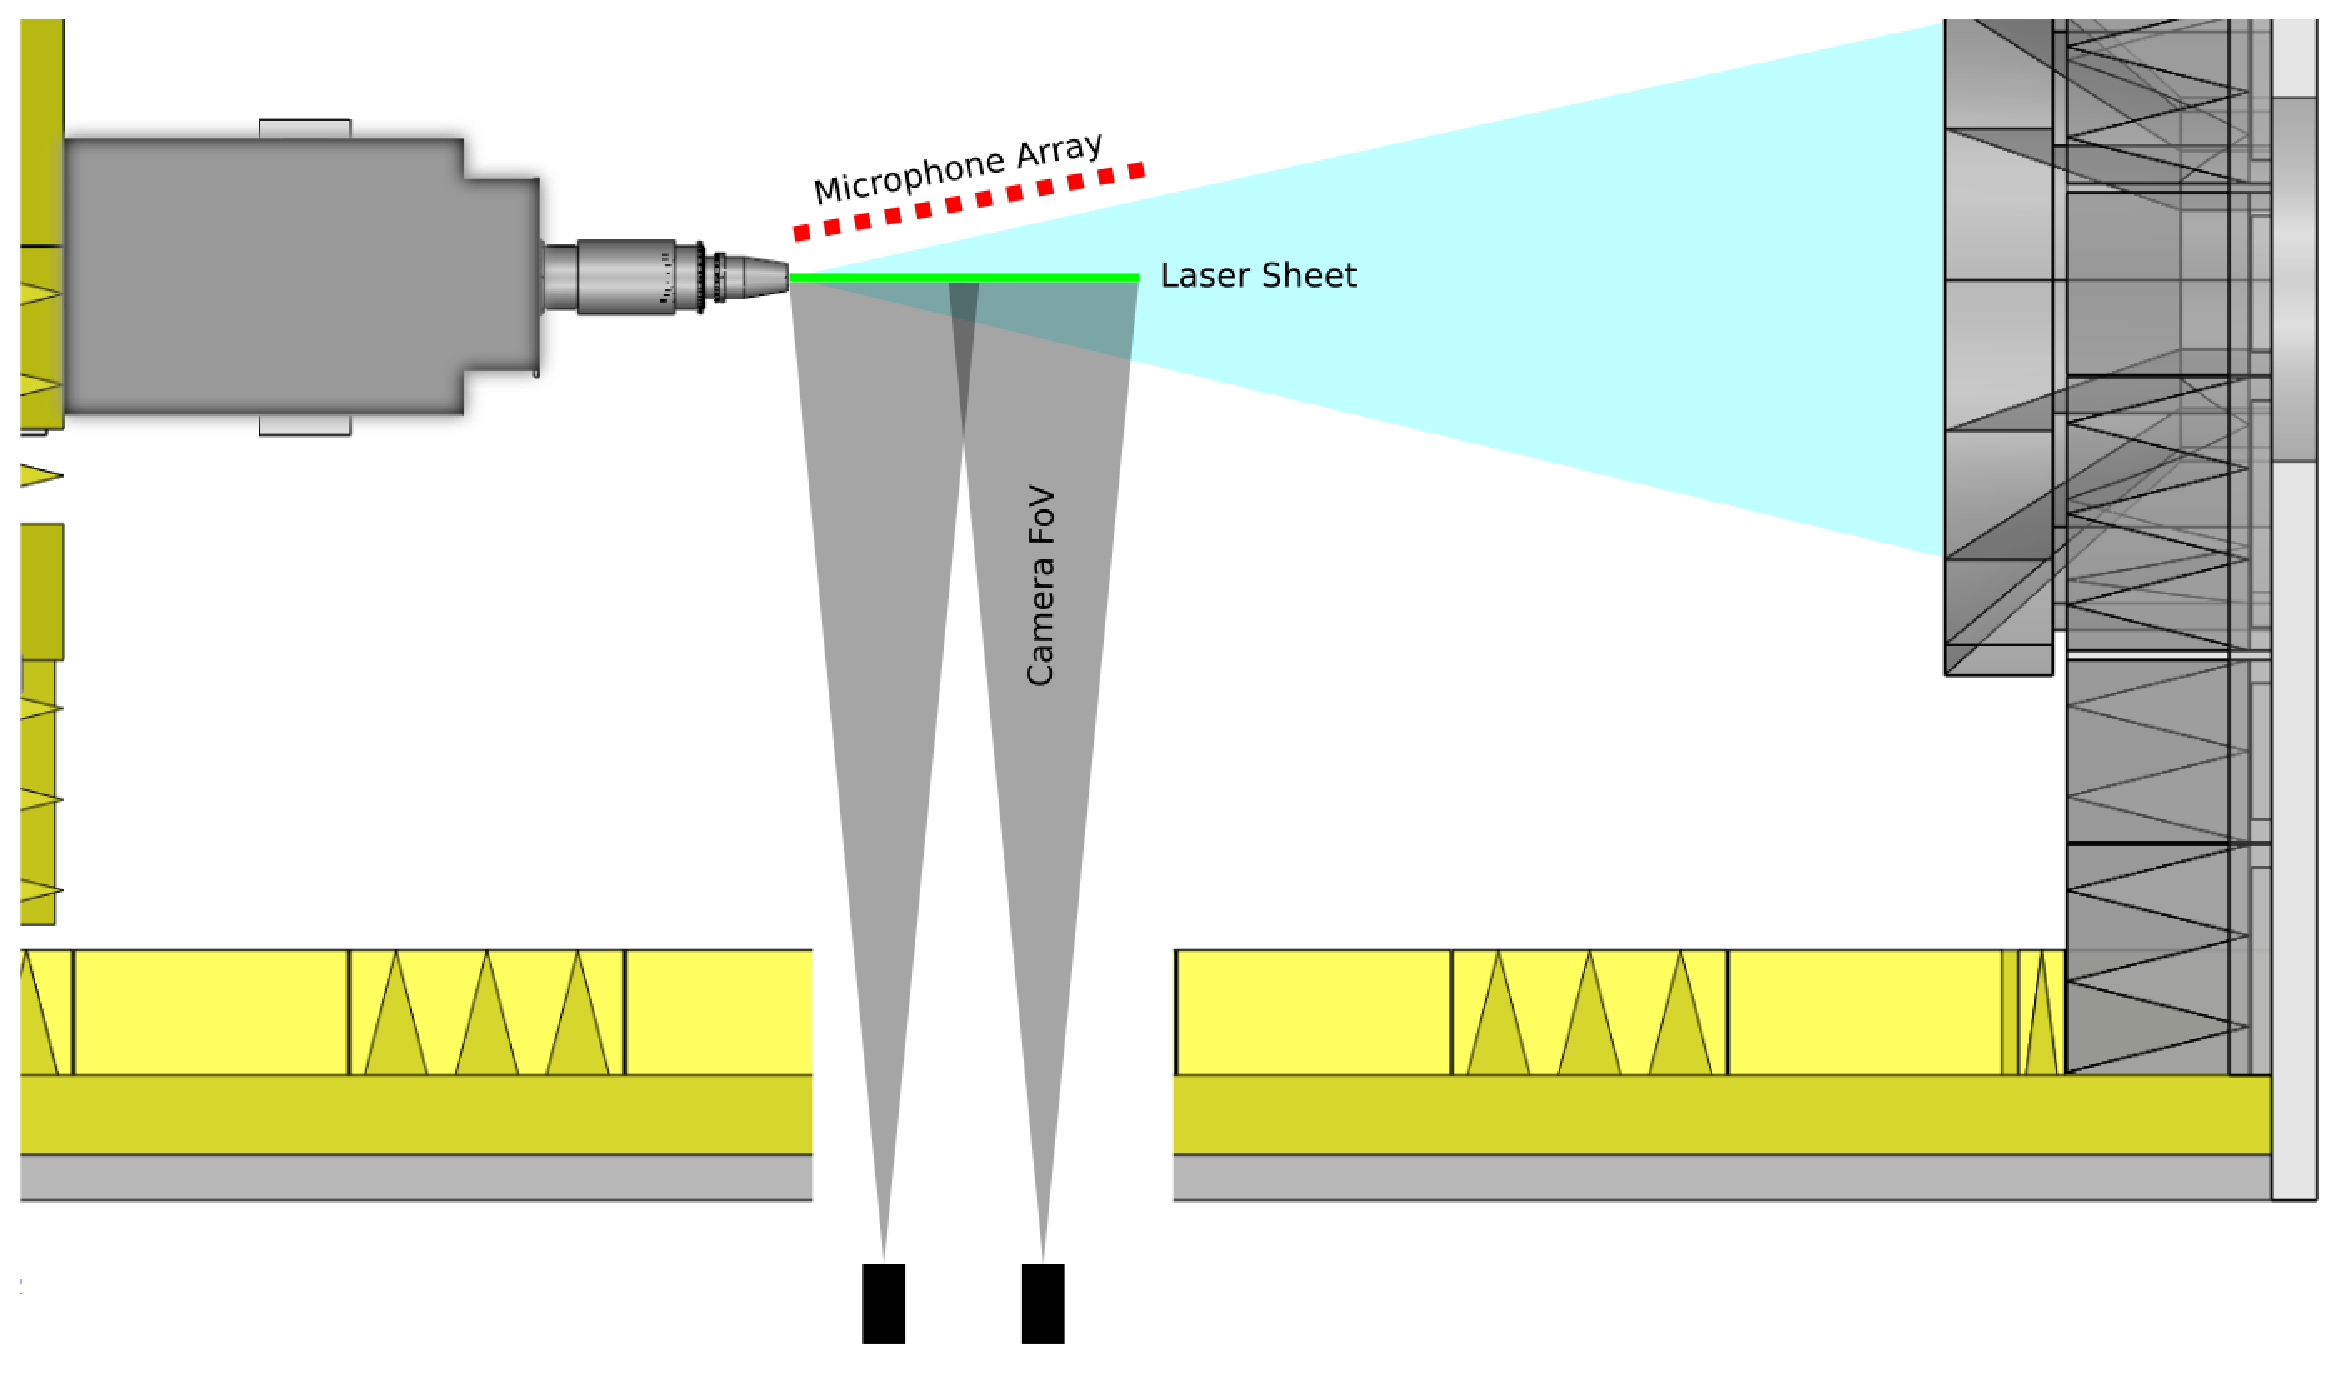
\includegraphics[width=4in]{Figures/ch2_piv_setup.eps}
	\caption{Schematic of syncronized PIV and near-field pressure data acquisition setup.}
	\label{fig:piv_setup}
\end{figure}

The image groups were acquired randomly in time at the system's maximum acquisition rate.
The PIV computer was set to output a reference signal which was used to trigger the acoustics data acquisition system.
The timing was set such that the PIV image acquisition would occur roughly in the center of a data block acquired by the acoustics system; the signal from a photoreceiver was also recorded in order to accurately identify the timing of the image acquisition in relation to the pressure time traces.
For this case, 1500 image groups were acquired for each case.
\section{The Near- and Far-field Response to Excitation}
\label{sect:nearfield}
\subsection{Periodic and Impulse Response}
The genesis for this project first began with the work of \citet{Sinha2012}, which studied the irrotational near-field response of a subsonic jet subjected to excitation with plasma actuators by decomposing the instantaneous fluctuating pressure field into a coherent `wave' component (which corresponds to the large-scale structure generated by the excitation) and incoherent residual fluctuations (which correspond to the natural turbulence in the jet). 
Fundamentally, this decomposition is similar to the triple decomposition used by \citet{Hussain1970}.
Sinha \etal found that each pulse from the actuators produces a coherent large-scale structure that would grow, saturate, and decay as it advects through the jet shear layer. 

In the irrotational near-field, the signature of these large-scale structures takes the form of a compact waveform. 
At low enough excitation frequencies, the characteristic period of this waveform is much less than the excitation period, and hence, the structures seeded by the excitation do not interact with one another as they evolve downstream. 
Therefore, their behavior can be thought of as representing the response of the jet to a single perturbation; in short this is the `impulse' response of the jet, which is produced by the impulsive excitation by LAFPAs.
As the period of actuation approaches the characteristic period of the impulse response, the waveforms extracted by the phase-averaging technique are largely unmodified from that of the impulse response. 
Above this frequency, significant interaction between the structures is observed, with noticeable modifications to the waveform shape and amplitude. 
As the structures are growing as they advect through the shear layer, the frequency at which the structures begin to interact is dependent on the axial location.
This behavior can be observed in \fig{fig:ch3_nearfield}a.
\begin{figure}
	\centering
%	\begin{subfigure}{.5\textwidth}
%		\centering
		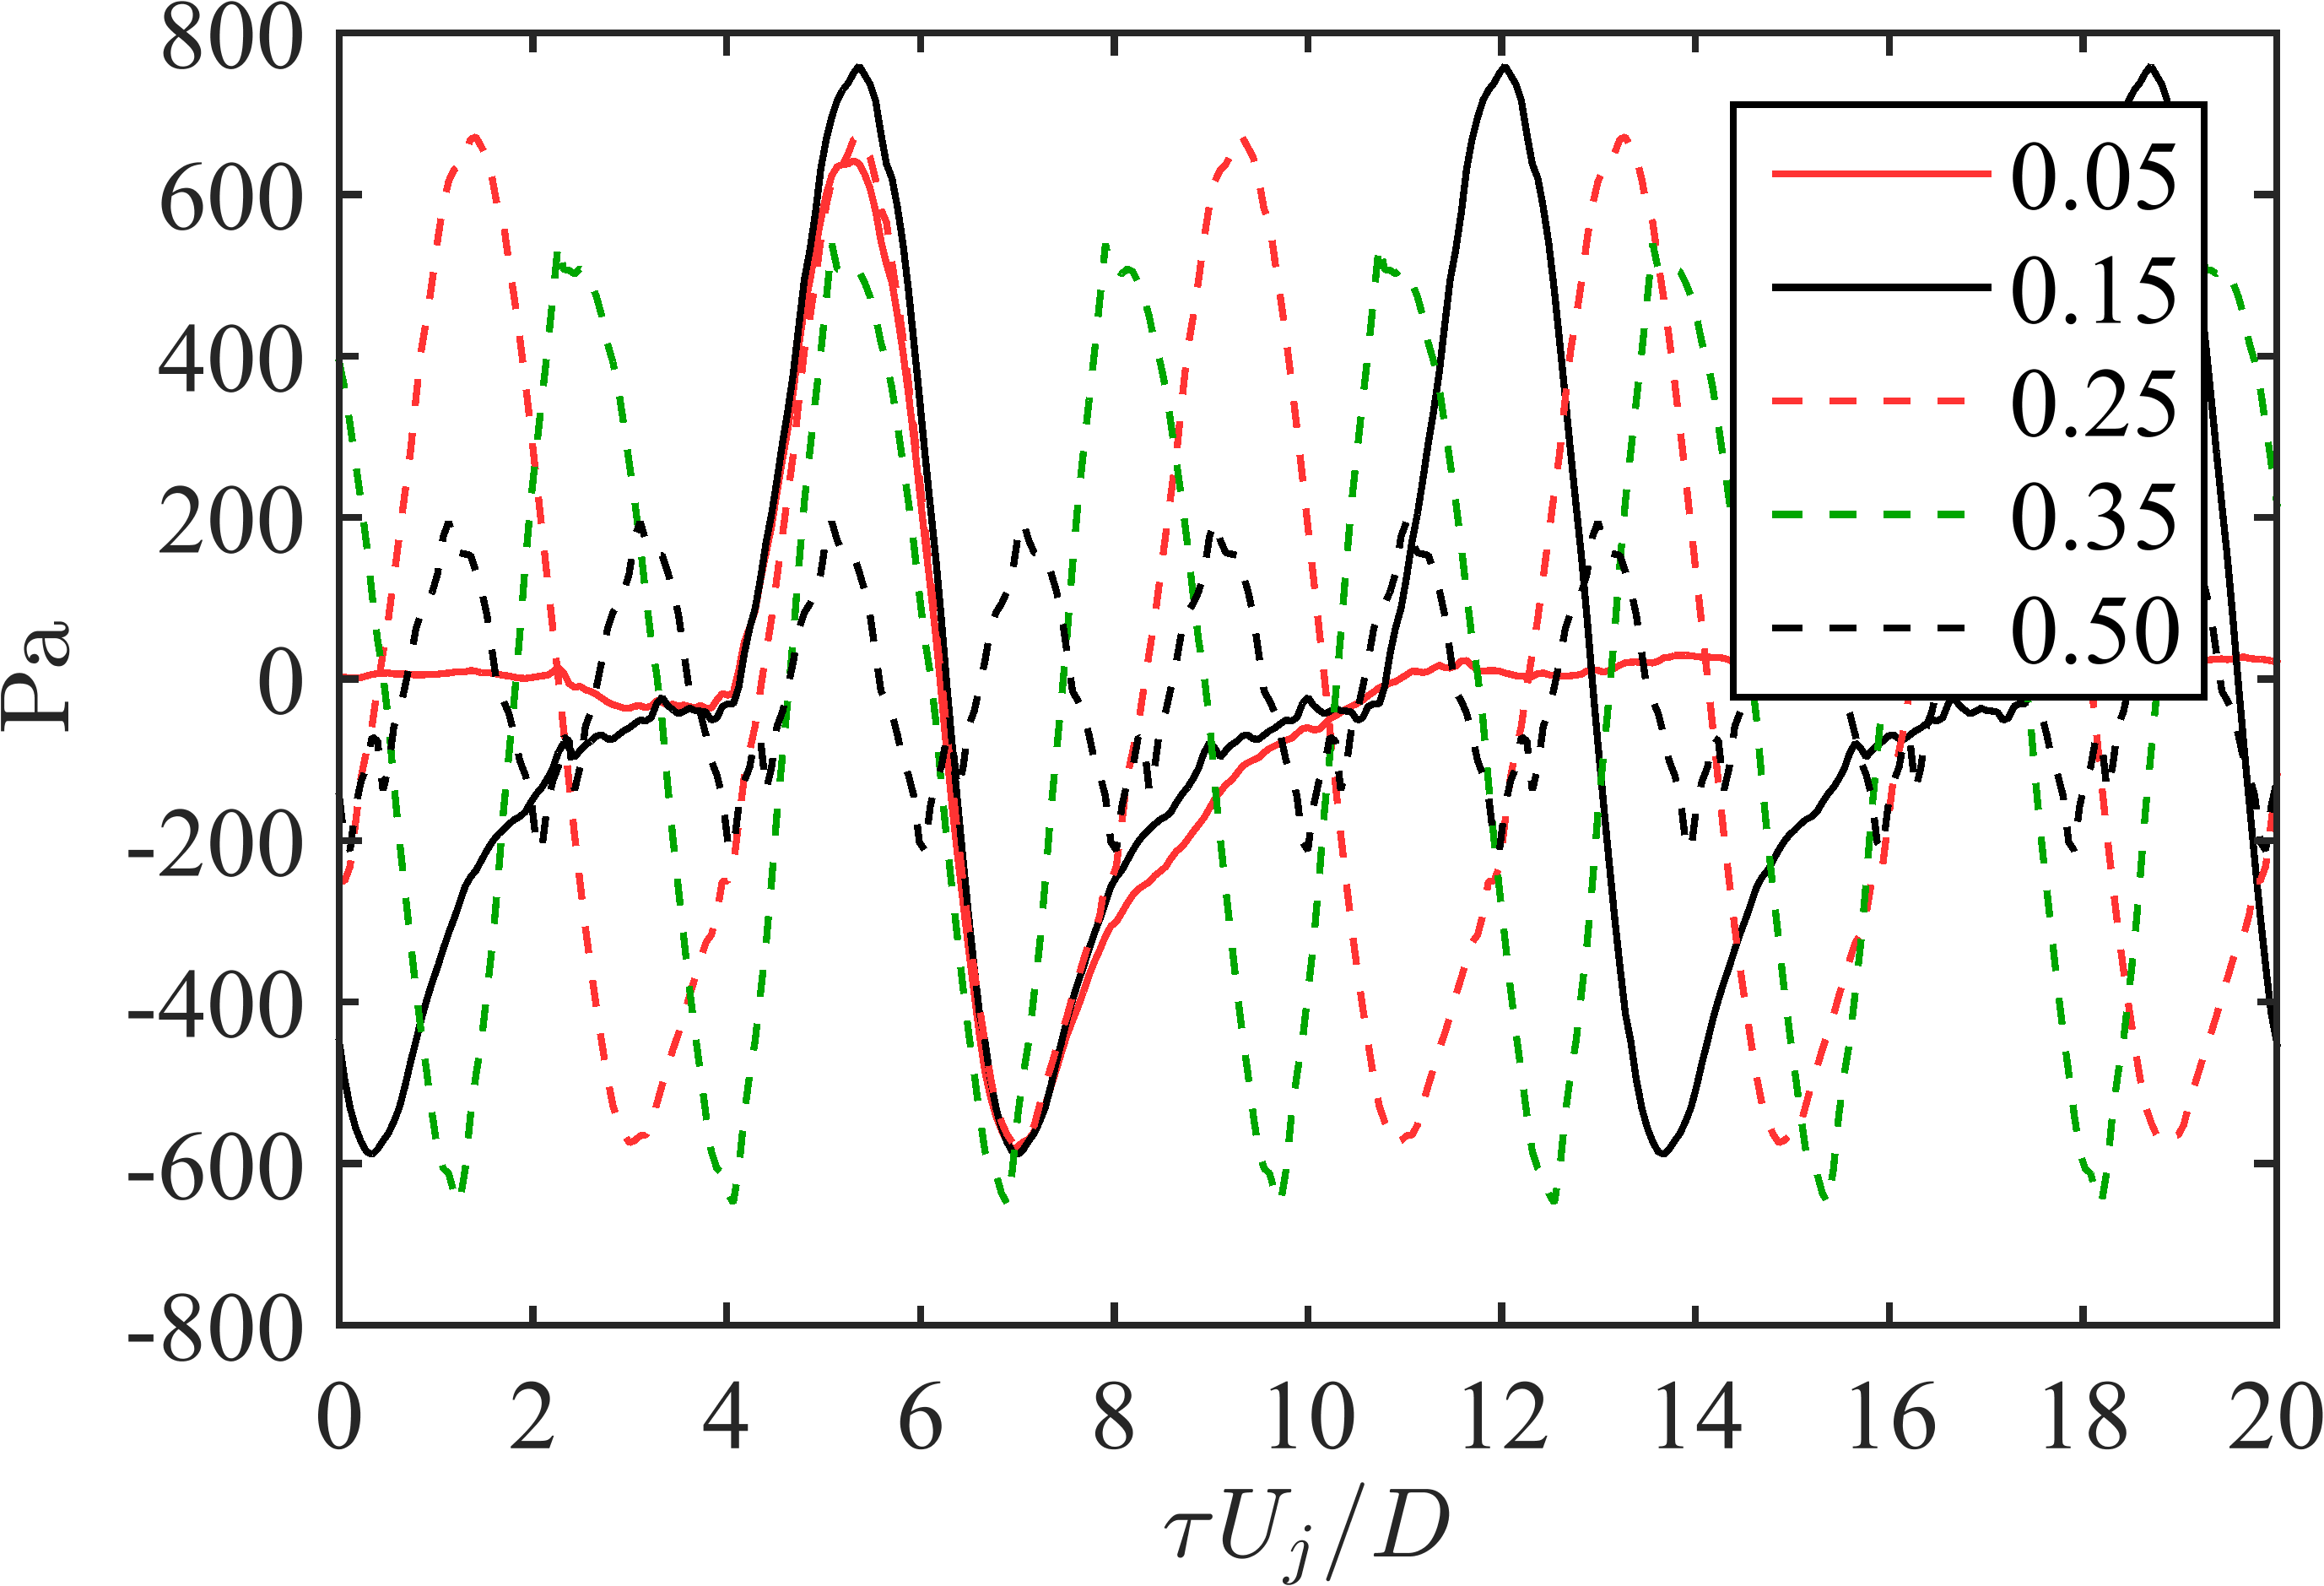
\includegraphics[width=0.45\linewidth]{Figures/ch3_nearfield_phavg_v2.png}
%		\caption{}
%		\label{fig:ch3_nearfield_phavg}
%	\end{subfigure}%
%	\begin{subfigure}{.5\textwidth}
%		\centering
		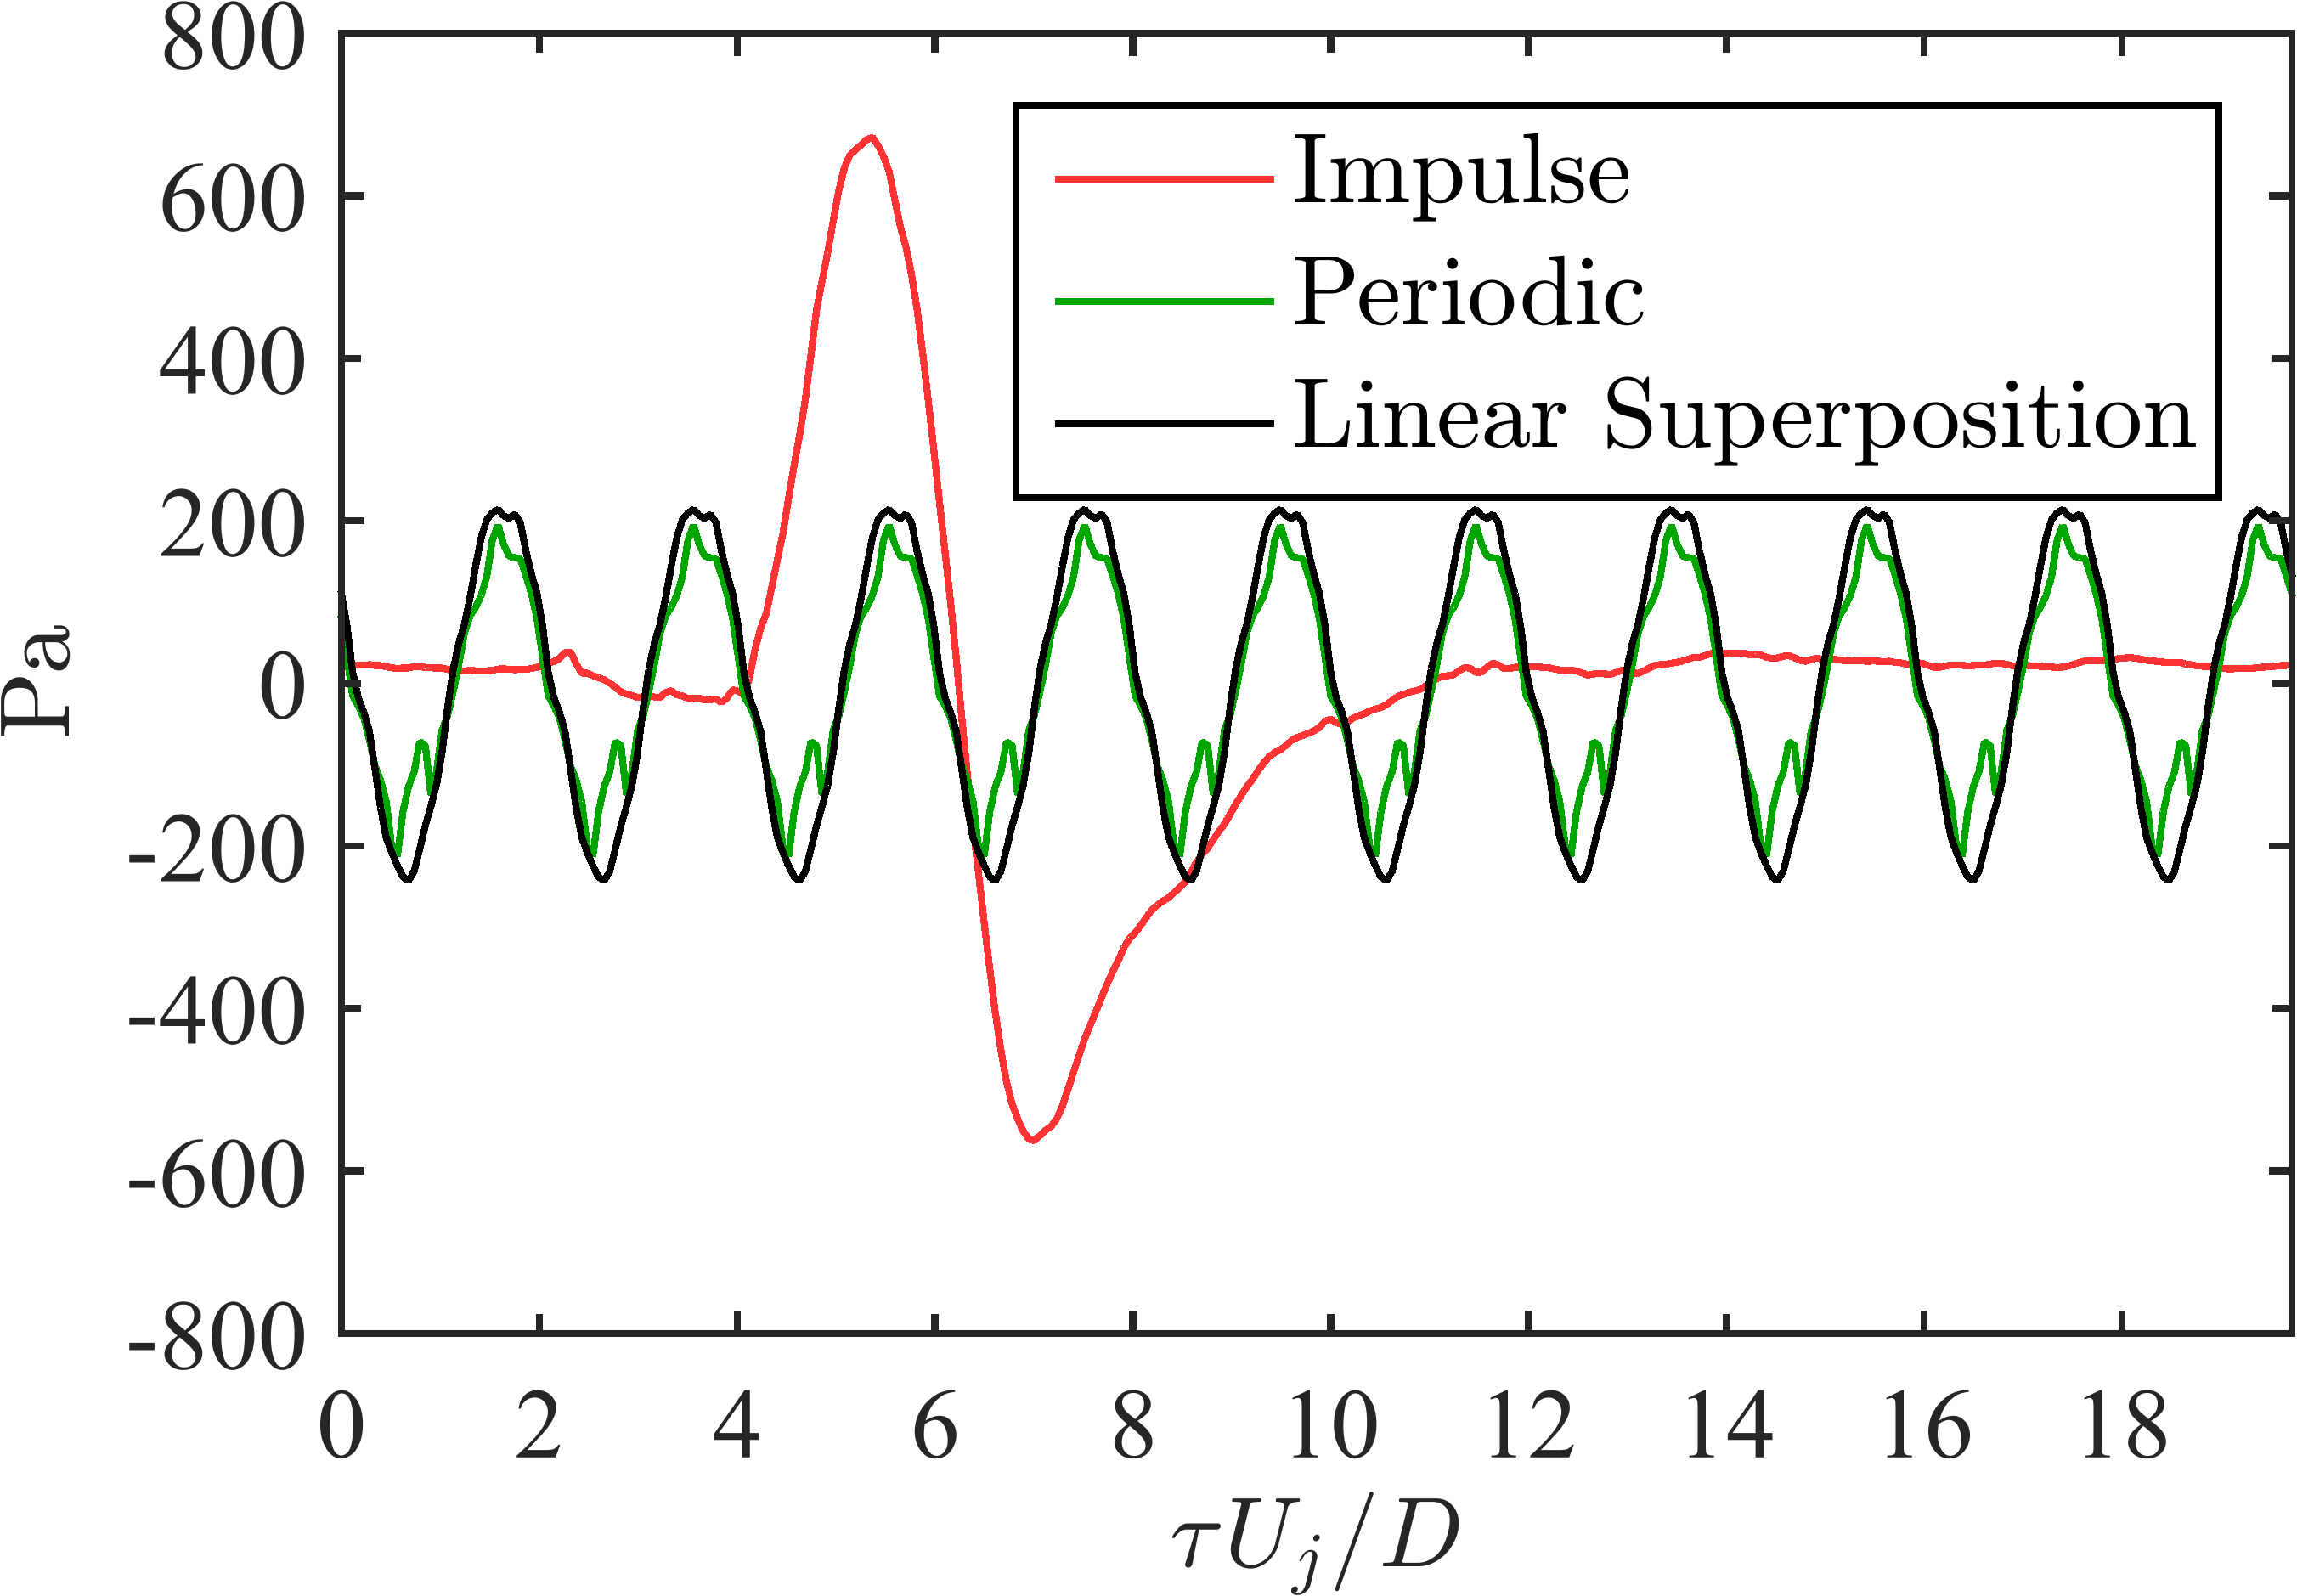
\includegraphics[width=0.45\linewidth]{Figures/ch3_nearfield_linear_v2.png}
%		\caption{}
%		\label{fig:ch3_nearfield_linear}
%	\end{subfigure}
	\caption{Phase-averaged waveforms along the first array position at $x/D = 3, r/D = 1.35$ (a) and a linear superposition of the phase-averaged waveform for the impulse excitation ($St_{DF} = 0.05$) compared against periodic excitation ($St_{DF} = 0.50$) (b).}
	\label{fig:ch3_nearfield}
\end{figure}

For a certain range of excitation frequencies ($St_{DF} \leq 0.50$ at $x/D = 2$, for example), the structures interact in a quasi-linear manner, insofar as their near-field pressure signatures are concerned. 
To be precise, the response of the jet in the irrotational near-field could be well-predicted by a linear summation of the impulse response of the jet, repeated at the periodic excitation frequency. 
This concept has been illustrated in \fig{fig:ch3_nearfield}b, where the periodic response of the jet to excitation with $St_{DF} = 0.50$ has been reproduced at $x/D = 3$. 
Additionally, a linear superposition of the impulse response for $St_{DF} = 0.05$, repeated to match the excitation frequency of $St_{DF} = 0.50$, has been overlaid. 
The linear superposition has been arbitrarily shifted in time in order to match the phase of the periodic response; this phase difference is likely due to the dependence of convection velocities on structure frequency \citep{Veltin2011} (or more accurately, structure size). 
For reference, the impulse response has also been included in the plots. 
Upstream of the end of the potential core ($x/D \simeq 6$, as will be found in \sect{sect:velocity}), the quasi-linear interaction model produces close predictions of the waveform amplitude and shape, despite the significant difference in both peak amplitude and waveform shape between the impulse and periodic responses. 

This quasi-linear interaction of the jet response to excitation is not limited exclusively to the hydrodynamically-dominated regions of the jet, but in fact holds for the acoustic far-field as well, at aft angles (where the acoustic signal is strongest and is known to correlate well with large-scale structures). 
This can be observed in \fig{fig:ch3_farfield}a, where the phase-averaged response of the jet has been plotted for the far-field signal at a polar angle of $30^\circ$. 
For legibility, only a select number of excitation Strouhal numbers have been included. 
As with the irrotational near field, the acoustic far field exhibits a compact waveform for the lowest excitation Strouhal numbers. 
Though nearly a direct inverse from the waveform observed in the hydrodynamically-dominated near field, the far-field waveform is quite reminiscent of the phase-averaged waveforms observed by \citet{Kambe1983} for the acoustic radiation towards aft angles produced by the head-on collision of vortex rings. 
At higher $St_{DF}$, a continuous oscillation between sharp expansion and compression waves is again observed, though the amplitude begins to decay above moderate excitation Strouhal numbers. 
\begin{figure}
	\centering
%	\begin{subfigure}{.5\textwidth}
%		\centering
		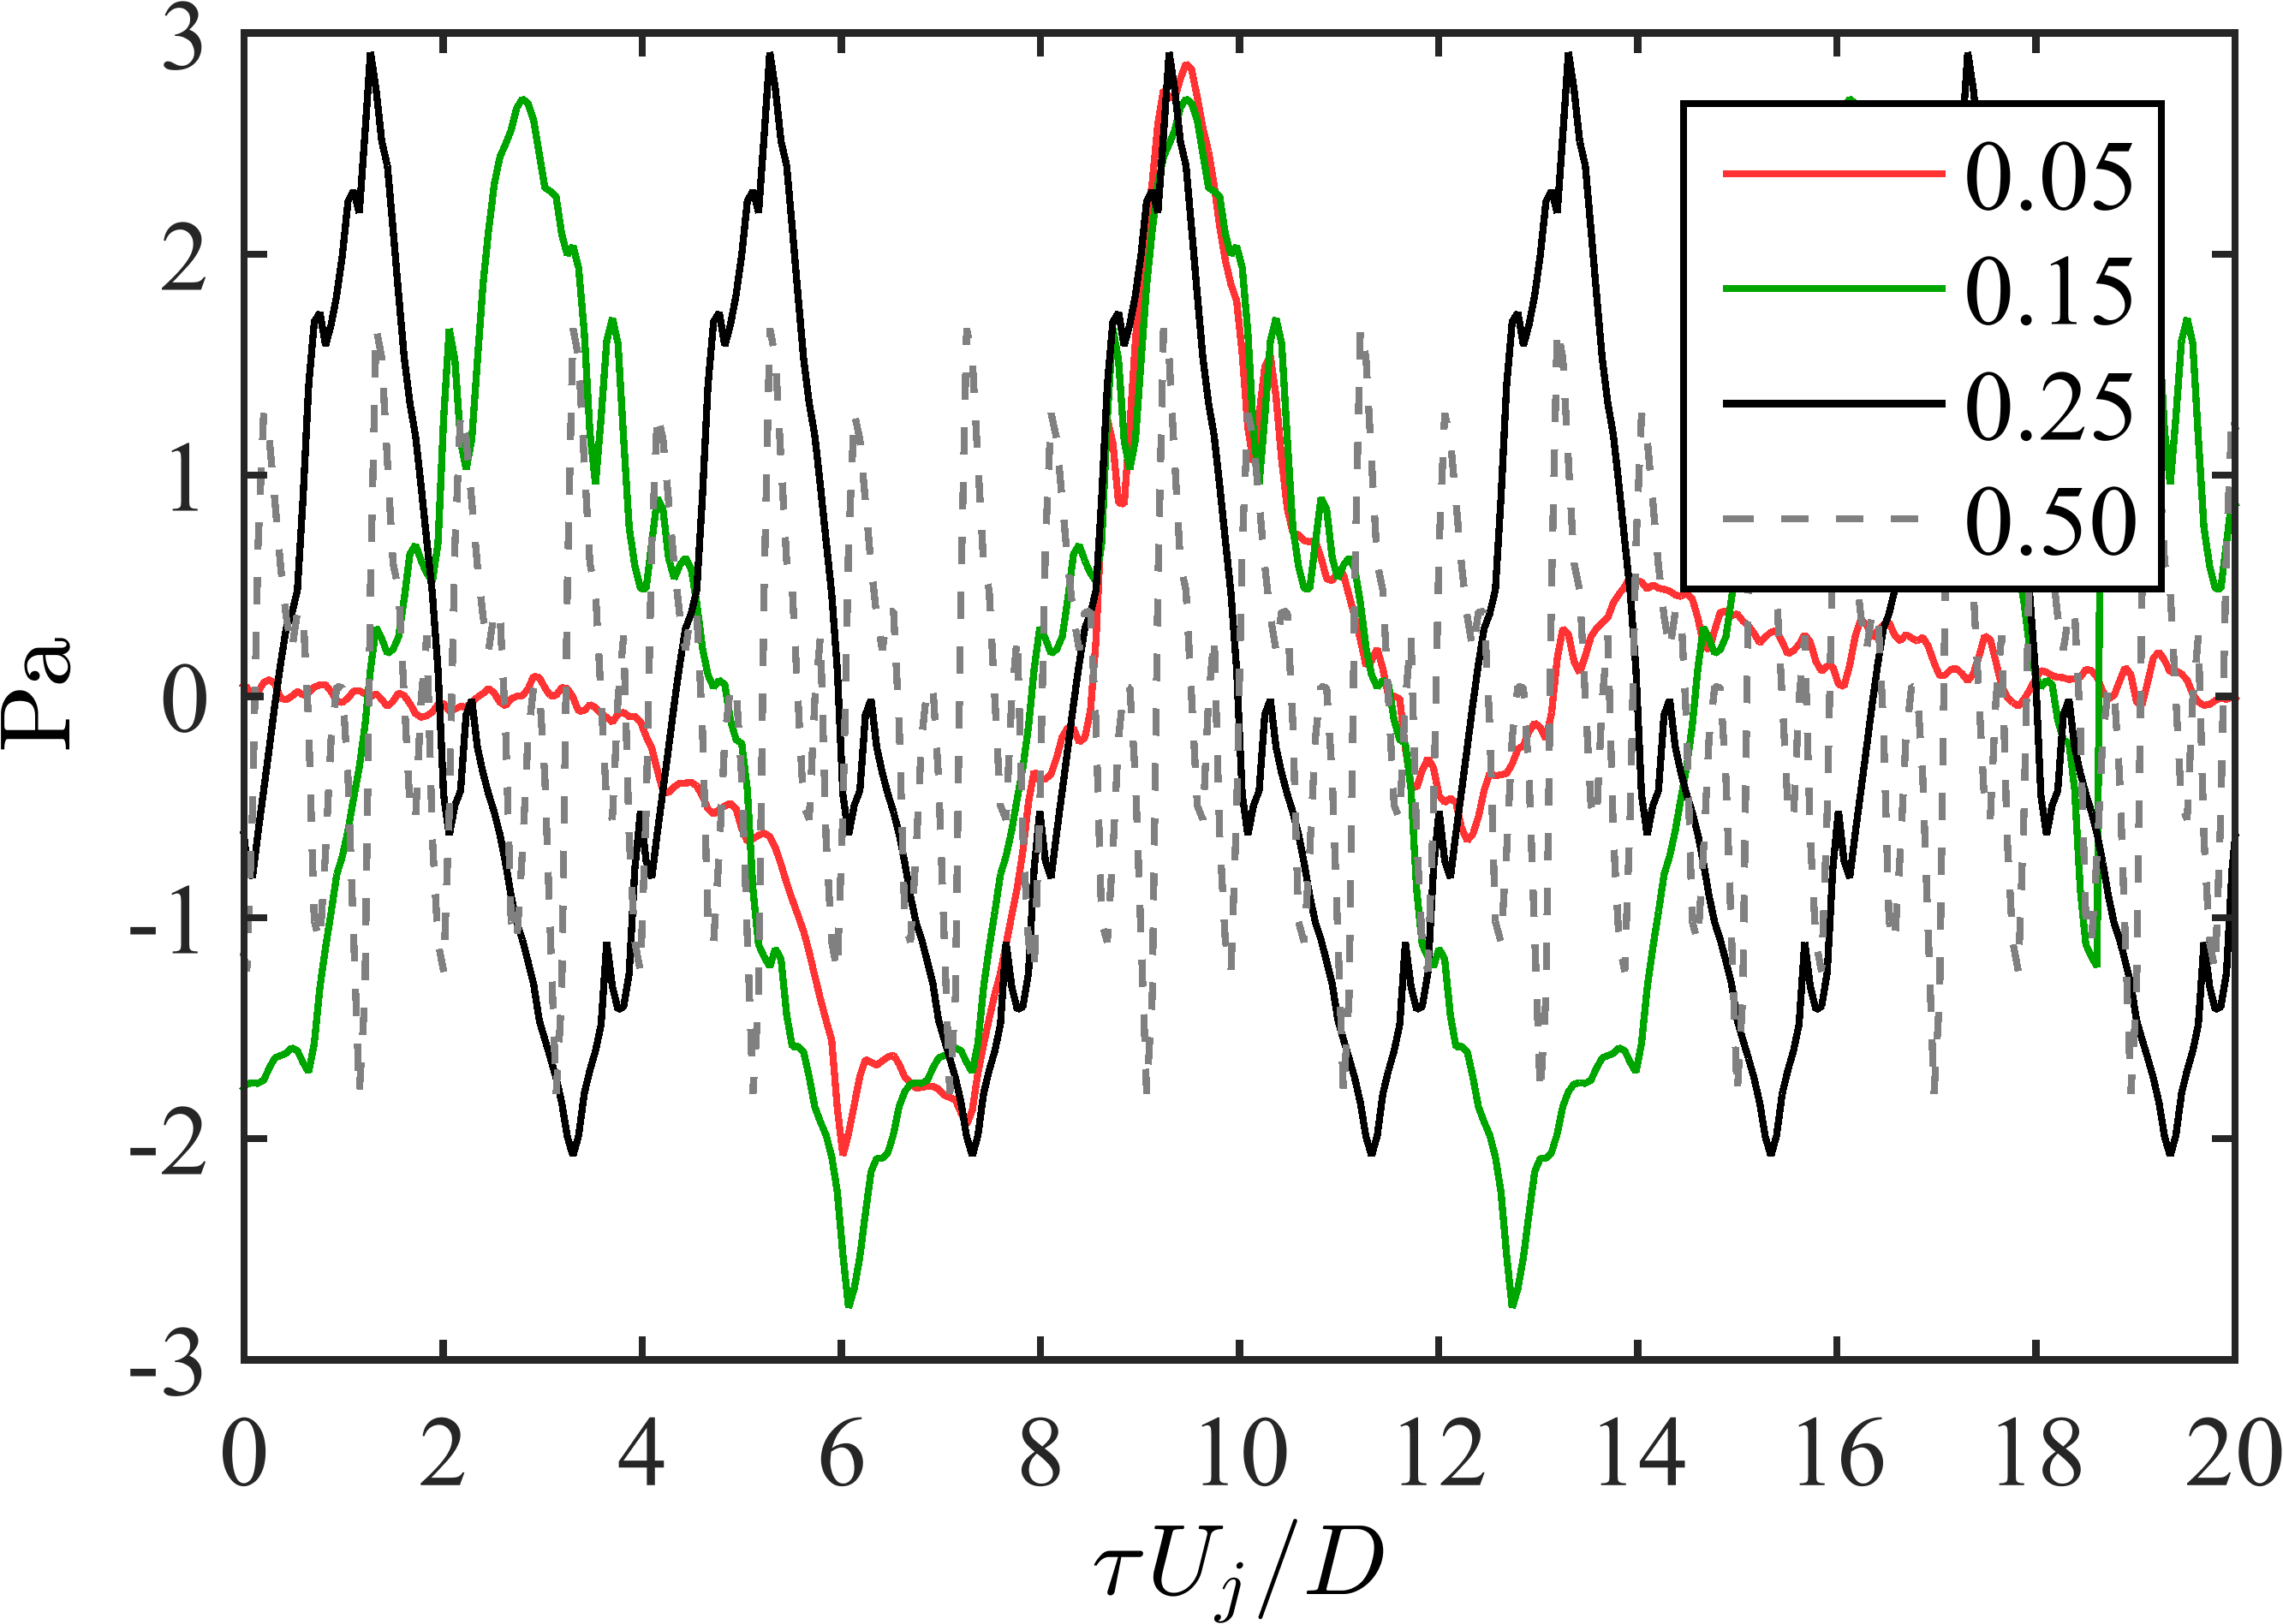
\includegraphics[width=0.45\linewidth]{Figures/ch3_farfield_phavg_v2.png}
%		\caption{}
%		\label{fig:ch3_farfield_phavg}
%	\end{subfigure}%
%	\begin{subfigure}{.5\textwidth}
%		\centering
		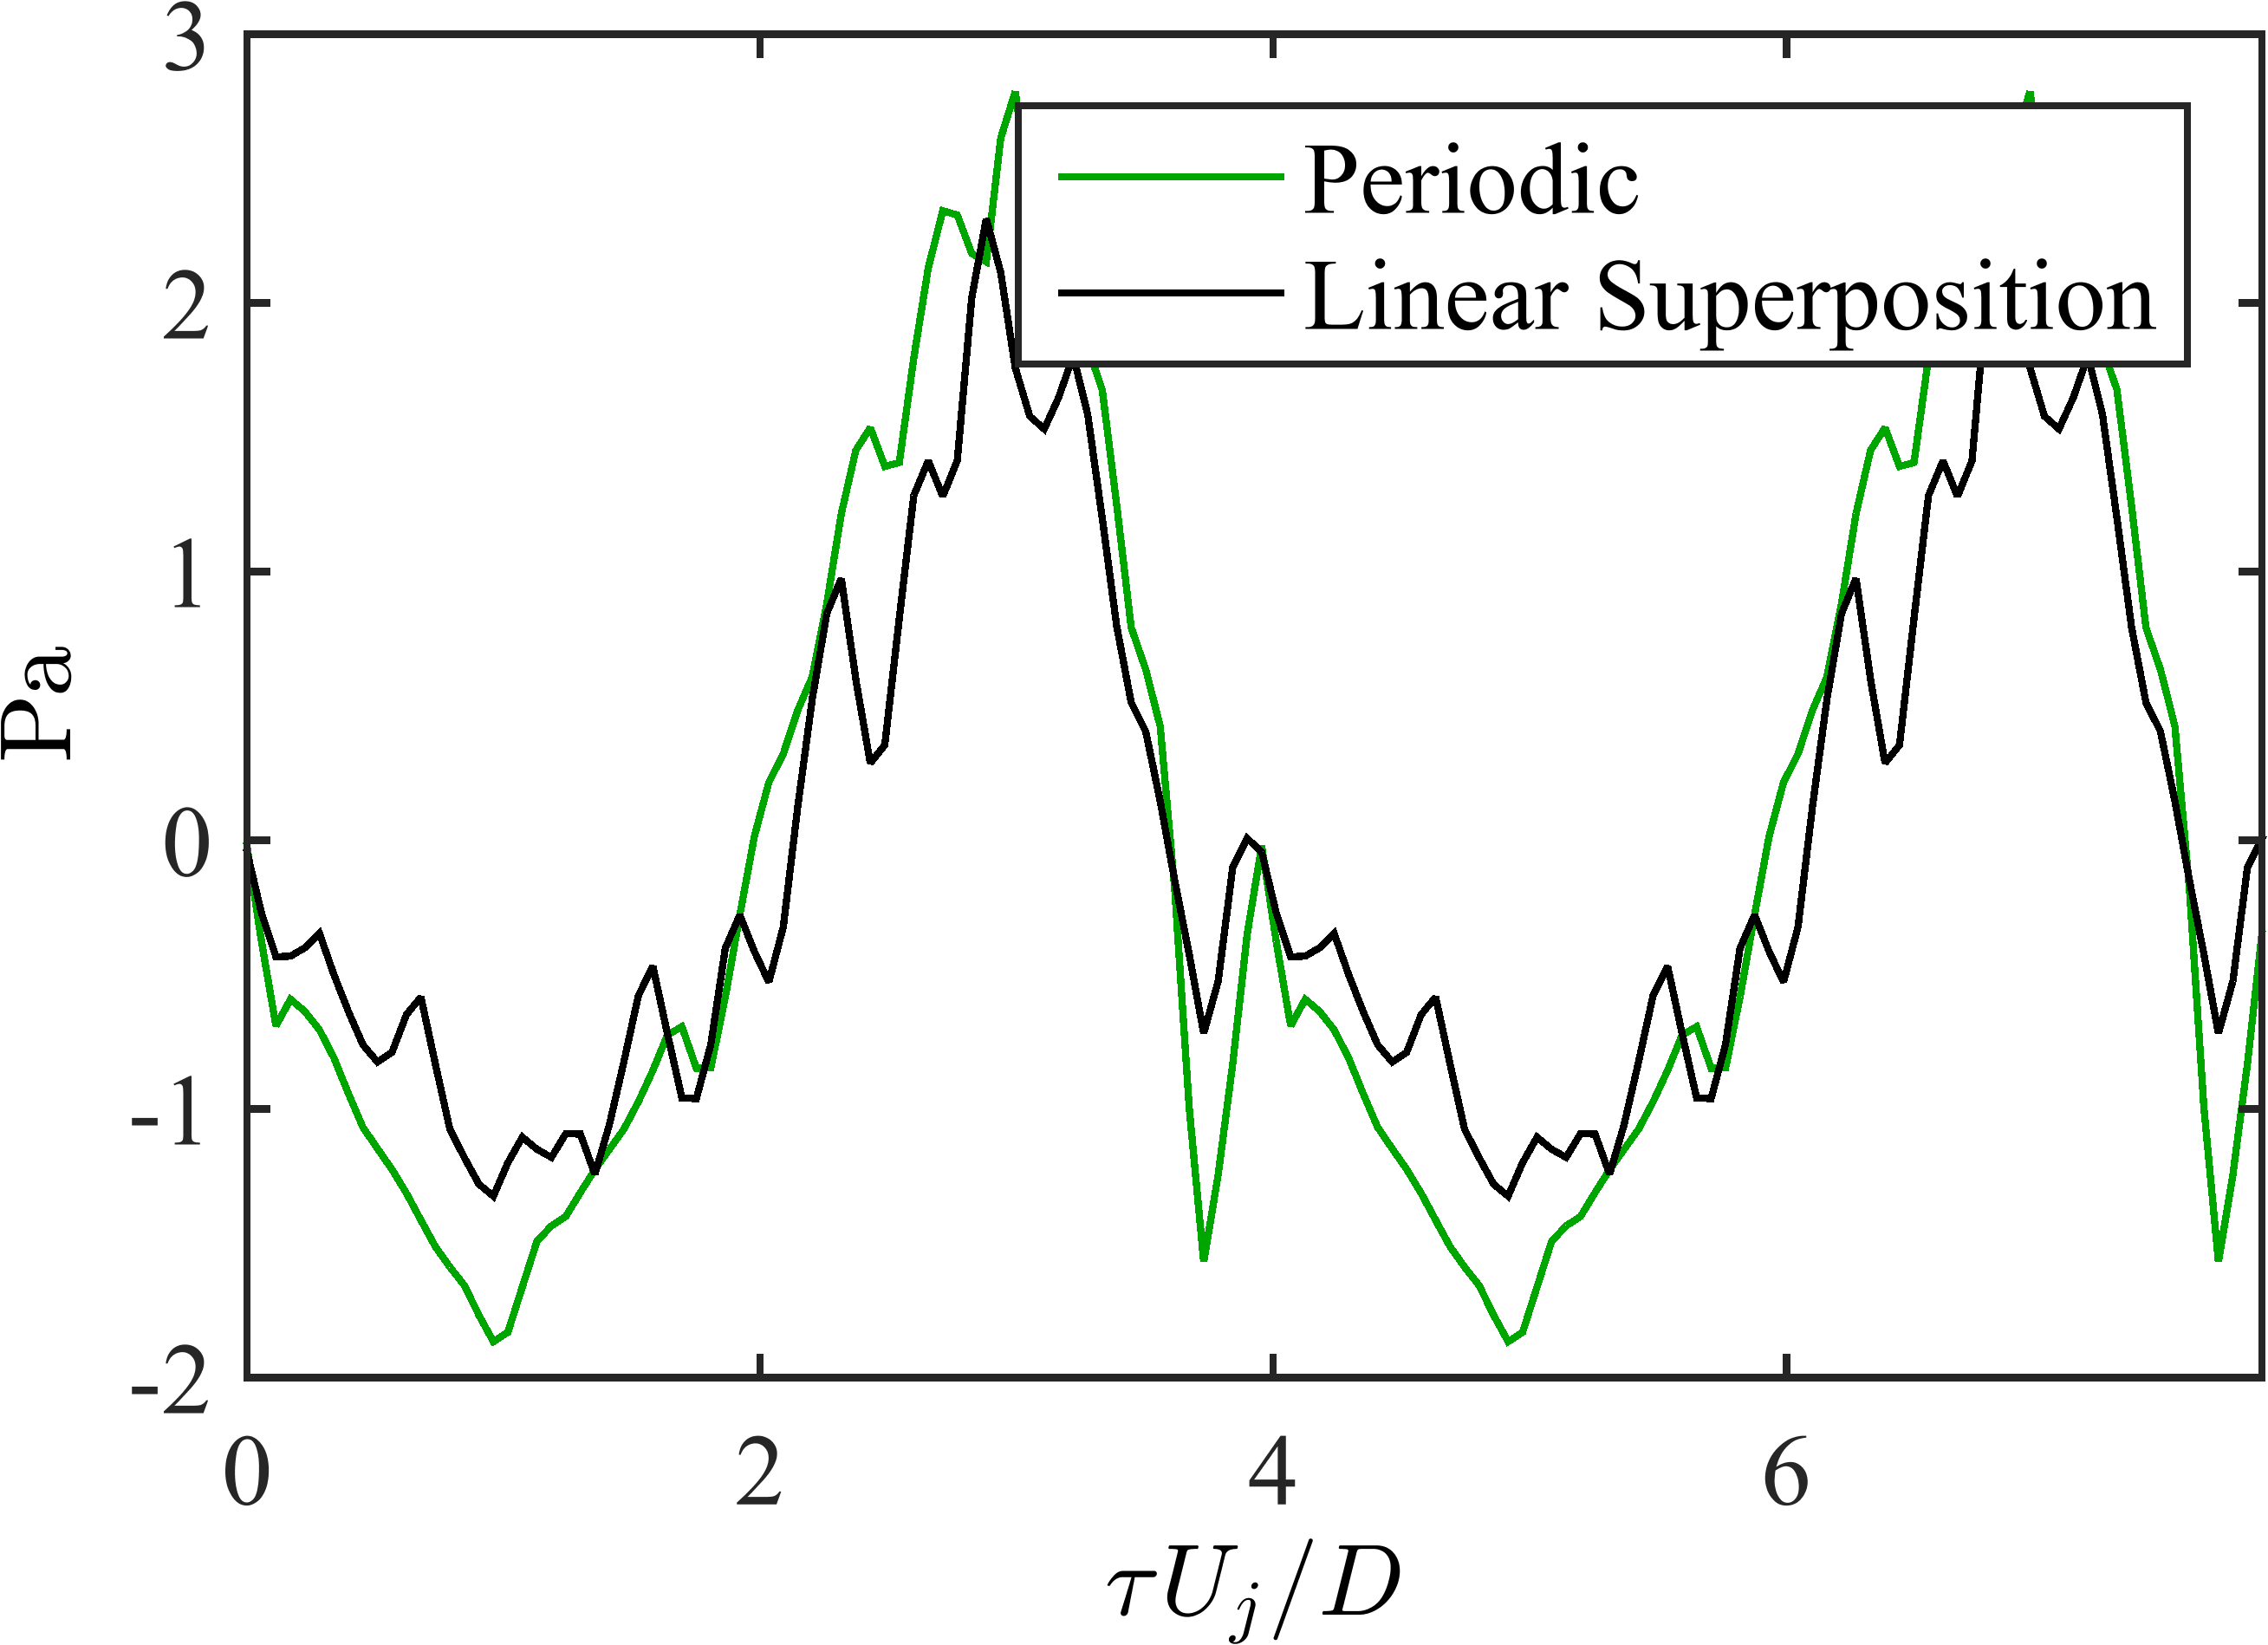
\includegraphics[width=0.45\linewidth]{Figures/ch3_farfield_linear_v2.png}
%		\caption{}
%		\label{fig:ch3_farfield_linear}
%	\end{subfigure}
	\caption{Phase-averaged waveforms of the far-field at $30^\circ$ (a) and a linear superposition of the phase-averaged waveform for the impulse excitation ($St_{DF} = 0.05$) compared against periodic excitation ($St_{DF} = 0.25$) (b).}
	\label{fig:ch3_farfield}
\end{figure}

As before, a linear superposition of the impulse response can well predict the waveform shape and amplitude at the higher excitation frequencies (\fig{fig:ch3_farfield}b), though in this case only up to $St_{DF}  = 0.25$. 
From the phase-averaged waveforms alone it is not clear whether this breakdown in the linear superposition model at the highest excitation frequencies is due to nonlinear behavior or uncertainty in the phase-averaging. 
Results comparing the linear superposition of the impulse response against the measured periodic response at $St_{DF}  = 0.35$ are shown in \fig{fig:ch3_farfield_nonlinear}.
Some similarities may be found in the waveform shape and amplitude, but overall it is clear that the acoustic response of the jet to excitation at $St_{DF}  = 0.35$ is substantially modified from the response at lower frequencies.
Though this is hardly conclusive in its own right, this result does suggest either changing or competing acoustic source mechanisms are present in these excited jets.
The phase-averaged waveforms were also investigated at polar angles of $60^\circ$ and $90^\circ$; however a clear waveform was not identifiable over the statistical uncertainty inherent in the phase-averaging process (likely due to the superdirective character of the acoustic radiation \citep{Crighton1990}, which renders the amplitude at sideline angles too low to be detectable).
Additional details and analysis of the phase-averaged near- and far-field signals can be found in \citet{Crawley2015}.
\begin{figure}
	\centering
	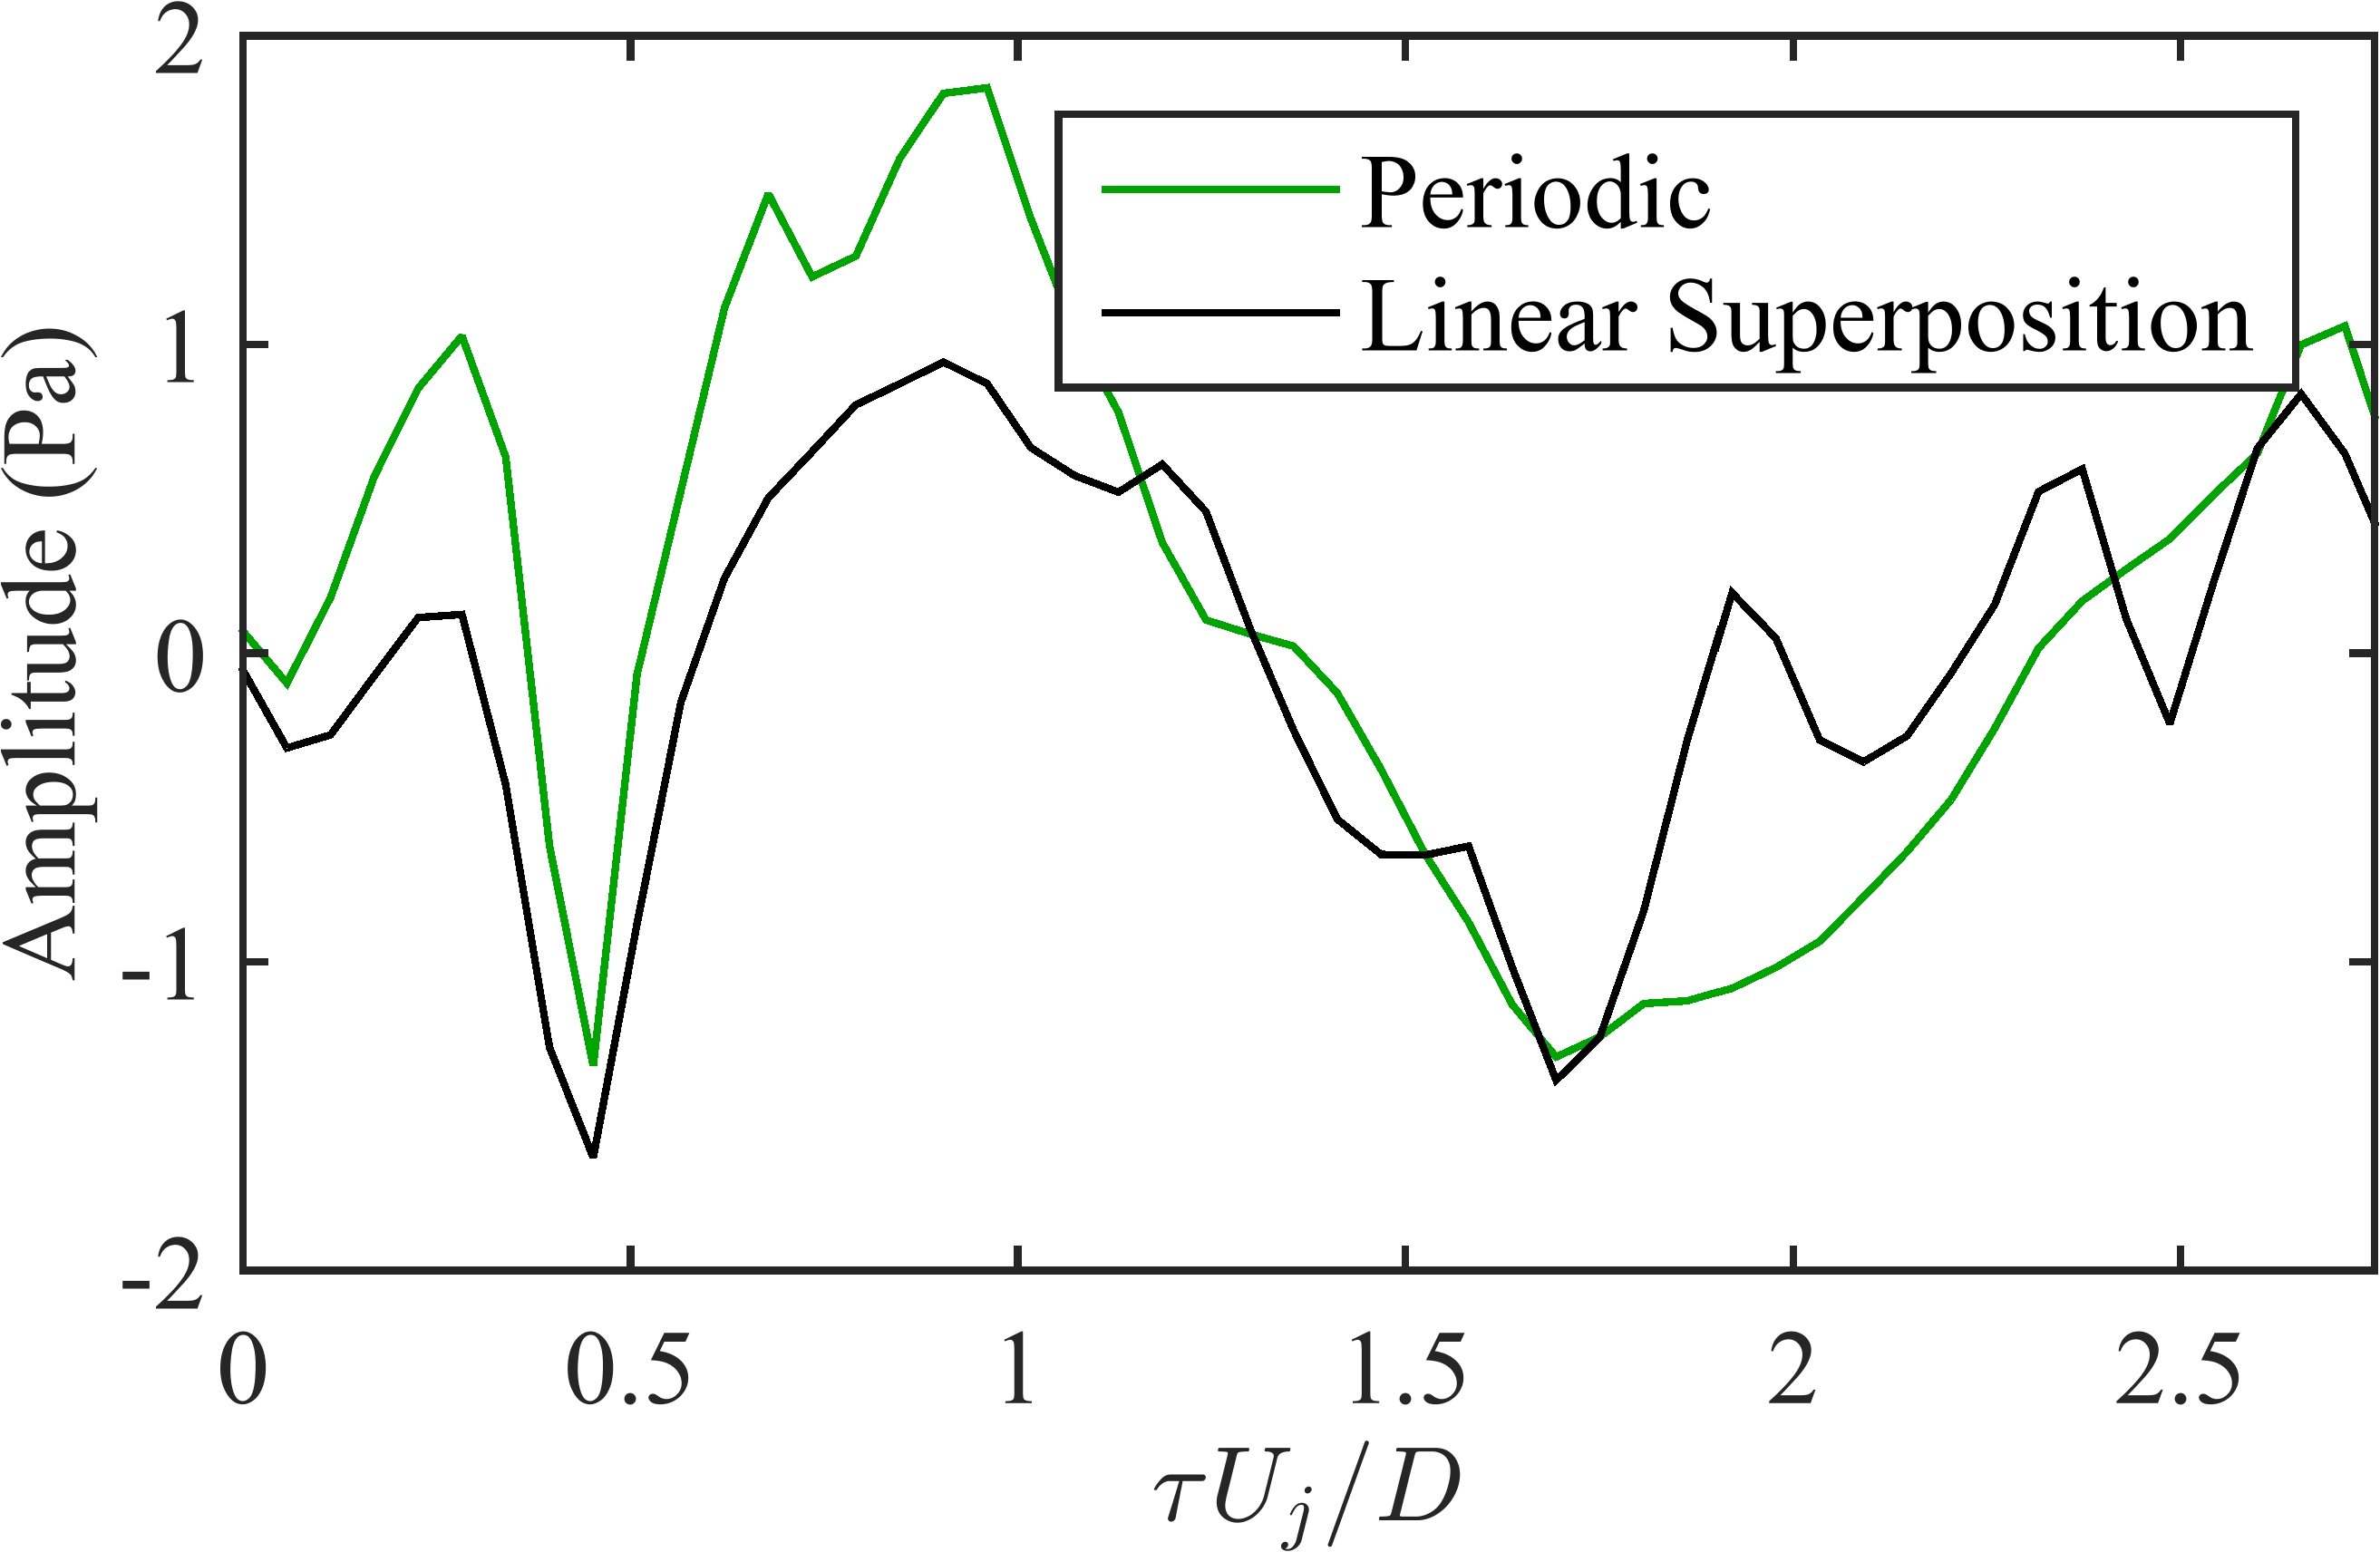
\includegraphics[width=0.45\linewidth]{Figures/ch3_farfield_linearsuperposition_st035_v2.png}
	\caption{Linear superposition of the phase-averaged impulse response to excitation against the measured periodic response for $St_{DF} = 0.35$ at the  $30^\circ$ far-field microphone.}
	\label{fig:ch3_farfield_nonlinear}
\end{figure}

\subsection{Excited versus Natural Structures}
The effect of excitation on the turbulent jet is to generate highly energetic coherent structures which persist downstream for several lengthscales.
As can be seen by the strong tonal energies observed for the excited jets in figure \fig{fig:sect_nearfield_spectra_prms}a, the near-field response to these structures contains energy at the fundamental excitation frequency and numerous higher harmonics.
As the excitation frequency increases from the impulse-excitation regime to the periodic, the dominance of the fundamental tone over the higher harmonics becomes more pronounced, though this is an artifact of the Fourier transform and not a fundamental physical phenomenon. 
The presence of these highly-energetic structures can also lead to an amplification of the broadband turbulence, over a wide band of frequencies both above and below the fundamental excitation frequency.
It also produces a continuous upstream shift in the root-mean-squared peak amplitude of the phase-averaged, as can be seen in \fig{fig:sect_nearfield_spectra_prms}b, with the maximum being obtained near $St_{DF} \simeq 0.3$ (which is commonly identified as the jet column instability frequency in natural jets).
However, the fluctuation intensities as a function of frequency in the excited jets saturate much further upstream than in the natural jet ($x/D \simeq 3$ for $St_{DF} \simeq 0.3$ rather than downstream near the end of the potential core at $x/D \simeq 6$).
In light of this issue, an investigation of the coherent structures in the natural jet and their comparison against the excited was deemed pertinent to the analysis of the excited structure dynamics.
\begin{figure}
	\centering
	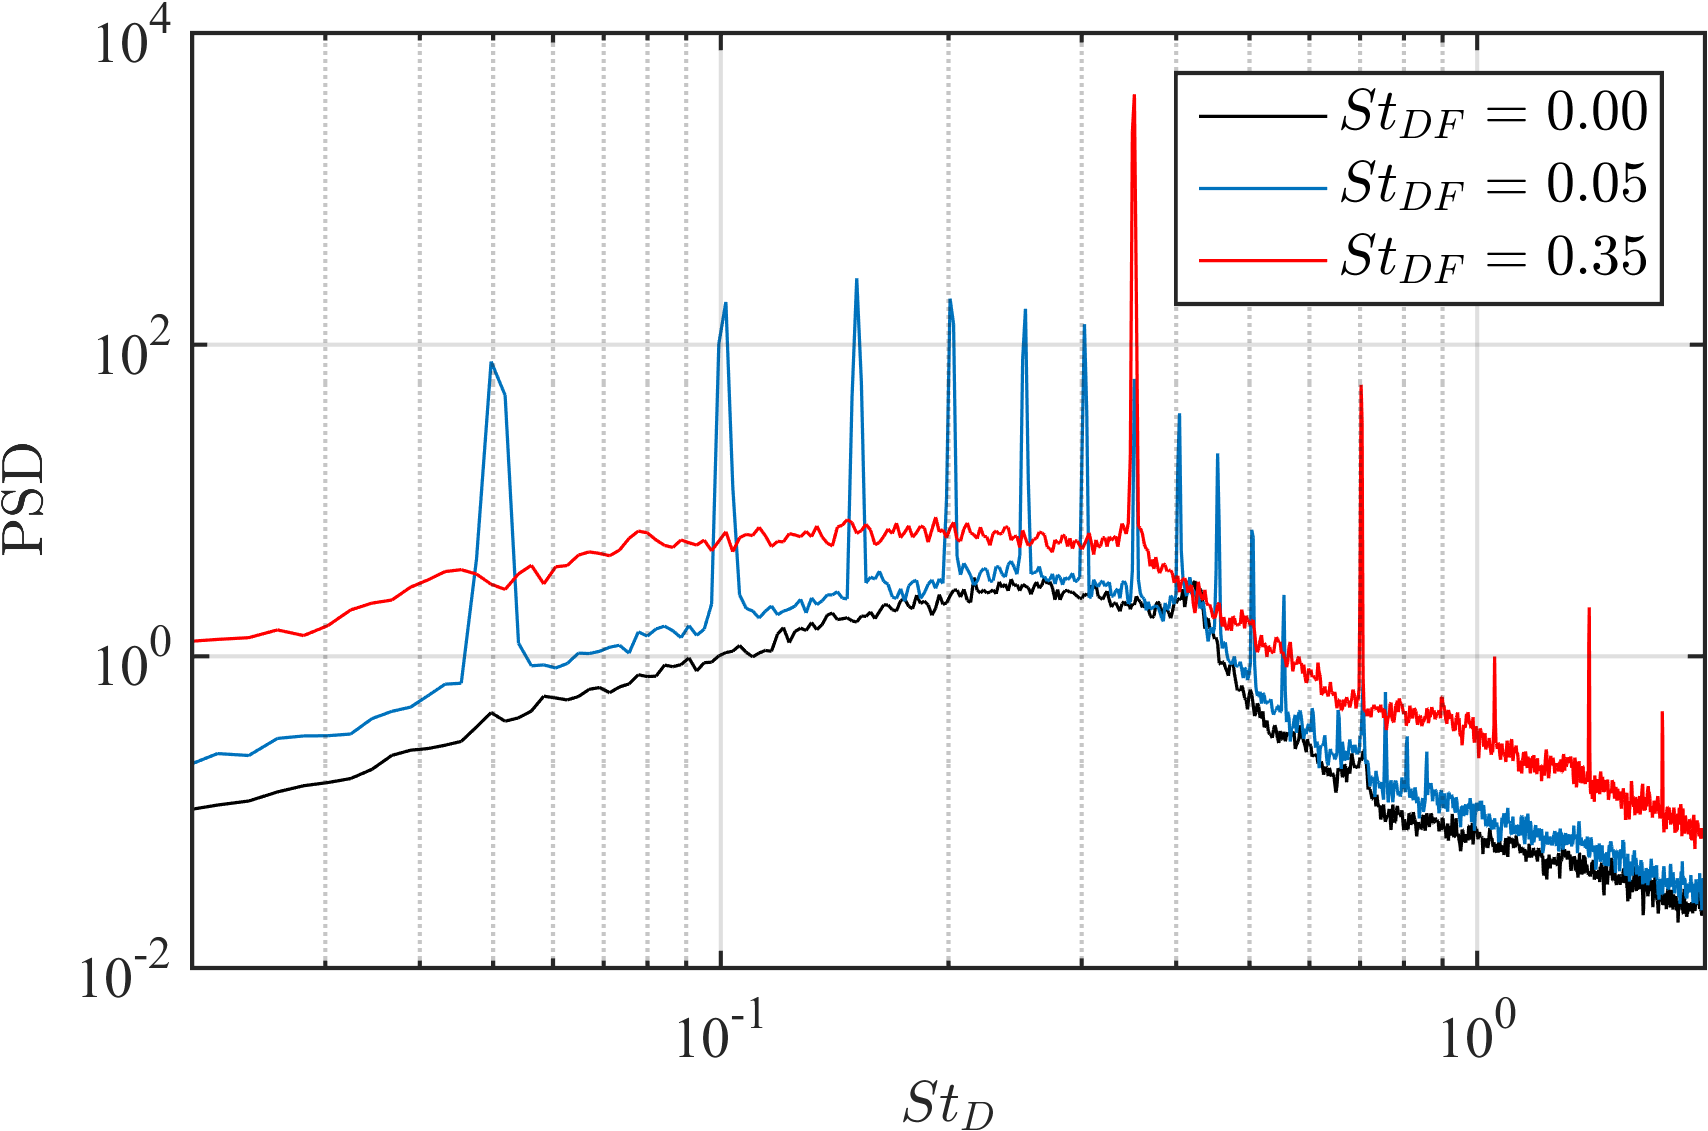
\includegraphics[width=0.44\linewidth]{Figures/sect_nearfield_spectra.png}
	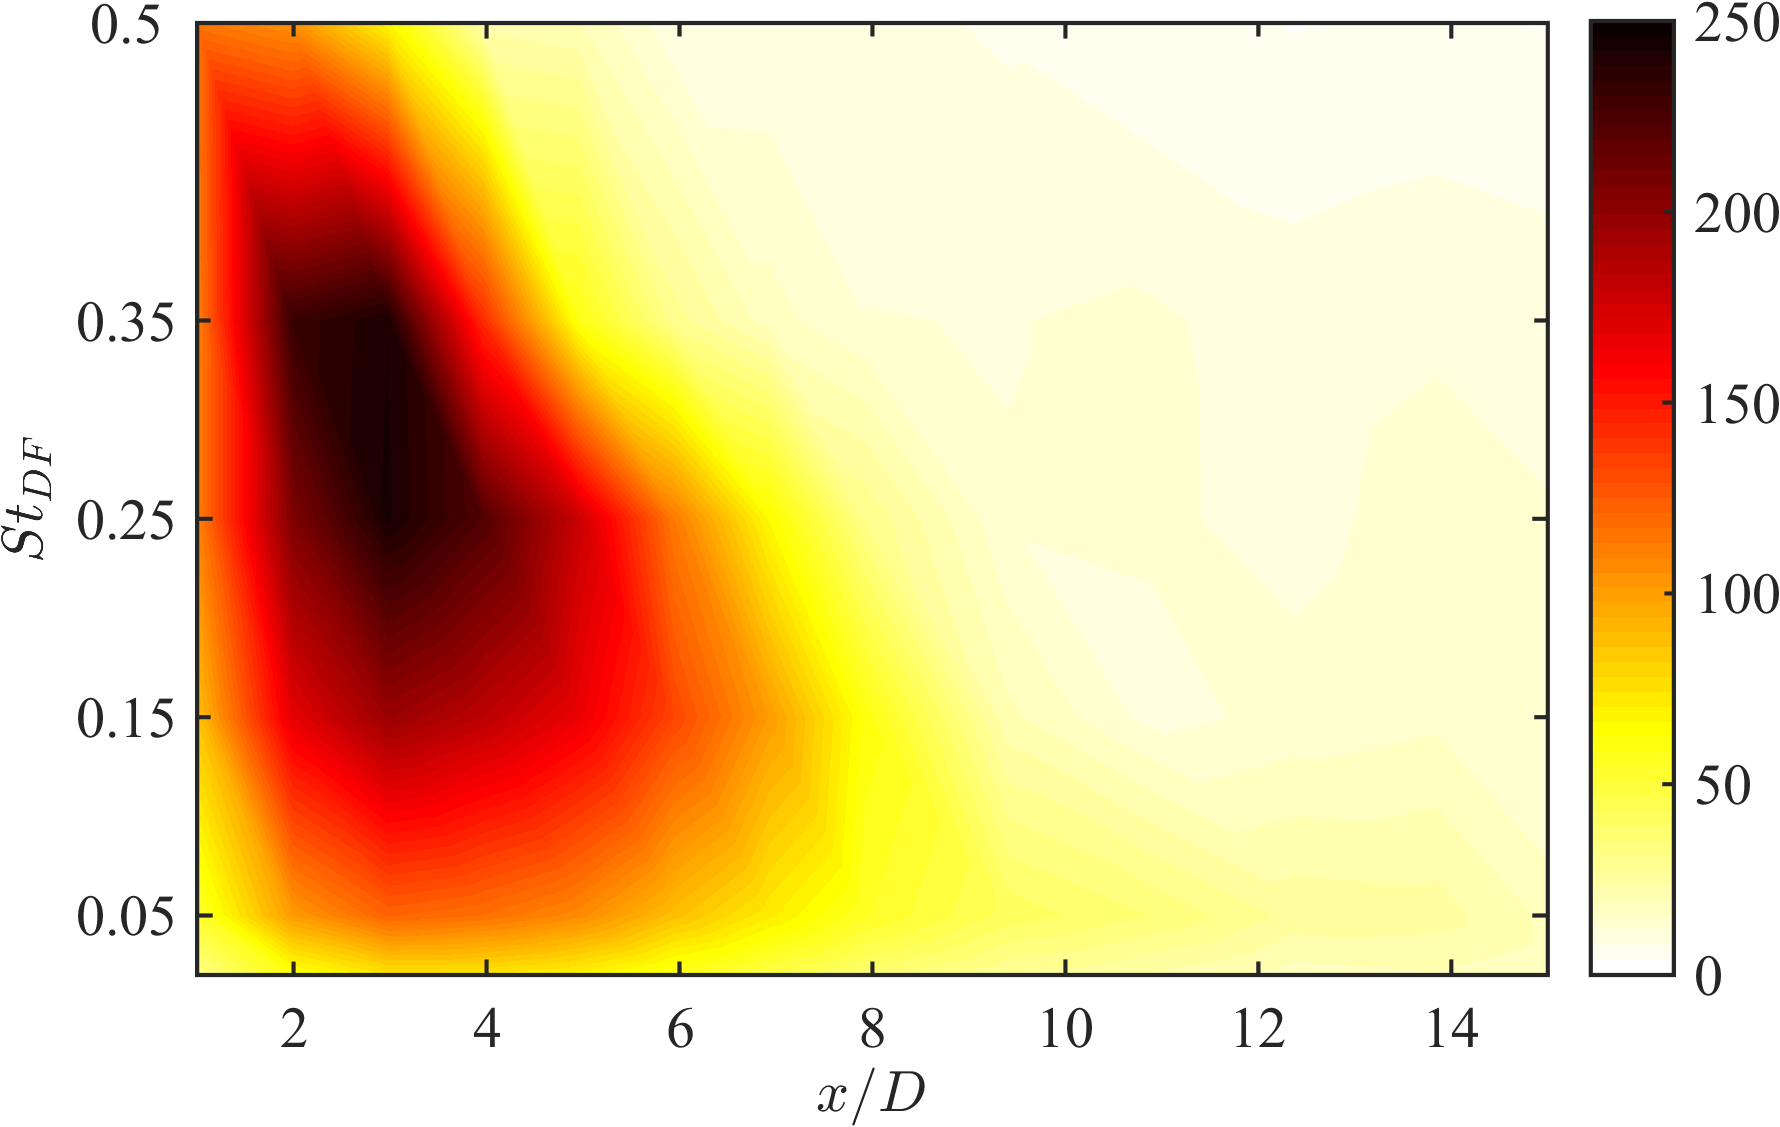
\includegraphics[width=0.46\linewidth]{Figures/sect_nearfield_prms.png}
	\caption{Power spectral densities of the raw near-field pressure at $x/D = 3$ (a) and root-mean-squared pressure fluctuations of near-field pressure at (b).}
	\label{fig:sect_nearfield_spectra_prms}
\end{figure}

Obviously, it is not possible to use standard phase--averaging with the unforced case since the natural turbulent structures, although dominated by Strouhal numbers related to the instabilities in the jet, contain a broad range of energetic scales with no fixed phase relationship. 
It is necessary then to use an alternative averaging method in order to extract a coherent signature of the unforced jet turbulent--structures.
Instead of phase-averaging a conditional--averaging method, specifically wavelet--conditioning, was applied to the unforced and forced cases to determine how closely the forced structures relate to the natural structures in the jet.
A wavelet decomposition was chosen as it affords an efficient methodology for analyzing intermittent events in a given signal due to the finite energy of its basis functions.
This is in contrast to the more standard Fourier decomposition in which continuously-oscillating basis functions spread information from a single instance in time across all transform coefficients.
For this reason, the use of the wavelet decomposition has become increasingly common in aeroacoustic research; an overview of the wavelet transform and its applications to turbulence and acoustics can be found in \citet{Farge1992}.
The wavelet decomposition is expressed as follow:
\begin{equation}\label{eqn:waveletDecomposition}
\tilde{w} \left( s, \tau \right) = \frac{1}{\sqrt{ \left| s \right|}} \int_{-\infty}^{+\infty} p \left( t \right) \overline{\Psi}\left( \frac{t - \tau}{s}\right) dt,
\end{equation}
where $s$ is the wavelet scale, which is inversely proportional to Fourier frequency, $\tau$ is the time--shift as in the Short Time Fourier Transform (STFT) formulation, $\overline{\Psi}$ is the complex conjugate of the so--called mother wavelet. The wavelet decomposition is as the STFT, a convolution of the signal to analyse with a family of functions, here the wavelets family. To get this wavelet family, which is also called the wavelet daughters, the mother wavelet is stretched/compressed and shifted. The strength of the wavelet decomposition with regards to STFT is the variation of the time--scale, which for STFT would correspond to its window. This allows a more localized information. In STFT the size of the window is fixed and the frequency is changing in order to retrieve the frequency content of the analysed signal while in the wavelet decomposition it is the time--scale (size of the window) which is different and the frequency is fixed. This difference allows to the wavelet decomposition to be more flexible and have a better resolution at both high and low frequencies.

%Wavelet--based conditional averaging has been used previously for structure identification in jets and other turbulent flows \citep{Camussi1997,Camussi1997b,Guj1999,Camussi2002,Guj2003}. % Need to add these refs to the bibtex, as professor Mike asked... XD
The technique is based on the Local Intermittency Measure (LIM) \citep{Farge1992}:
\begin{equation}
\label{eqn:LIM}
L(s, \tau) = \frac{\tilde{w}^{2}(s, \tau)}{\left<\tilde{w}^{2} (s, \tau)\right>_{\tau}},
\end{equation}
%where $w^{2}(s, \tau)$ is the local energy for a specific time and scale, and $\left< \bullet \right>_{t}$ represents a time average. Simply put, the LIM is the ratio between the local energy of the wavelet coefficient for a specific time and scale $(\tau, s)$ and a time-averaged energy at the same scale $s$. The LIM was demonstrated to be a well-suited indicator for coherent structure identification \citep{Camussi1997}.  The LIM provides information about the instantaneous fluctuation of energy and by choosing a proper threshold $T$ it is possible to select a set of times $\{\tau_{i}\}$ corresponding to intermittent, energetic events in a signal.

%Several methods exist in order to select the threshold: using an arbitrary threshold, an iterative process to retrieve as specific value of the Flatness Factor (skewness, forth moment), or by evaluating the Merit index \citep{Grassucci2015}. 
In the present study, a new method inspired by the merit coefficient was used to select a proper threshold. 
In contrast to the merit coefficient method, which uses a global threshold across all scales, the new method iterates at each scale to identify the proper threshold per \eq{eqn:tEvaluation}

\begin{equation} \label{eqn:tEvaluation}
R(T) = -\frac{\log\left(\frac{N_p}{N_m}\right)}{\log\left(\frac{\sigma_{w_p}}{\sigma_{w_m}}\right)}.
\end{equation} 
% \begin{enumerate}
% 	\item Select a first threshold to initiate the iterative process (1 in the present case)
% 	\item Evaluate the coefficient
% 	\begin{equation}
% 	R(T) = -\frac{\log\left(\frac{N_p}{N_m}\right)}{\log\left(\frac{\sigma_{w_p}}{\sigma_{w_m}}\right)}
% 	\end{equation}
% 	\item Re-evaluate $T$
% 	\item Iterate points 2 and 3 until $T$ achieve the maximum of $L$ for the scale under analysis
% \end{enumerate}
where $N_p$ is the length of the set $\{L > T\}$, $N_m$ is the length of the set $\{L \leqslant T\}$, $\sigma_{w_p}$ the standard deviation of the set $\{w\left( \tau_p\right) | L\left( \tau_p \right) > T\}$ and $\sigma_{w_m}$ the standard deviation of the set $\{w\left( \tau_m\right) | L\left( \tau_m \right) \leqslant T\}$.
The outcome of this iterative process is a set of vectors: one containing the different value of $T$ and the second the different value of $R(T)$. The threshold for the analysis is selected to correspond to the maximum of $R(T)$.

The next step is to get similar results to those obtained with the phase--average. In order to get the signatures, a conditional--average (\eq{eqn:ensembleAverage}) using the set of times $\{\tau_{i}\}$ is performed. In one way, the conditional--average and phase--average are similar: the set of times $\{\tau_{i}\}$ replaces the phases on which the phase--average is performed. At each time location corresponding to a peak of energy, a window $W$ of fixed time--length $l_{W}$ is selected from the original signal $p \left( t \right)$. The conditional--average, $\tilde{p}$ is calculated from this set of windows:
\begin{equation} \label{eqn:ensembleAverage}
	\tilde{p}^n_{m}\left( W \right) = \left< p_{m} | P_{k} \right>_{\tilde{\tau}^n_{s}} = \frac{1}{N^n} \sum^{N^n}_{i = 1} p_{m}\left(\xi_{i}\right),
\end{equation}
where the superscript $n$ and subscript $m$ stand for the position of the reference signal and of any other signal of the array, respectively. Also, the subscript $s$ stands for the scale, $N^n$ is the number of detected events, $\tilde{\tau}^n_{s}$ is the set of corresponding times for a specific scale $s$ at which these events are occurring and $\{\xi_{i}\}$ is the interval surrounding each peak, $\xi_{i} \in \left[ \tilde{t}_{i} - \frac{l_W}{2}, \tilde{t}_{i} + \frac{l_w}{2} \right]$, $\tilde{t}_{i} \in \tilde{\tau}^n_{s}$.
A first analysis using \eq{eqn:ensembleAverage} was performed on the microphones line--array. A second analysis was then performed by doing the conditional--average only with peaks with negative/positive value in the real domain (pressure).

\begin{figure}
	\centering
	\includegraphics[width=0.45\linewidth]{Figures/negativePeak.eps}%
	\includegraphics[width=0.45\linewidth]{Figures/positivePeak.eps}\\	
	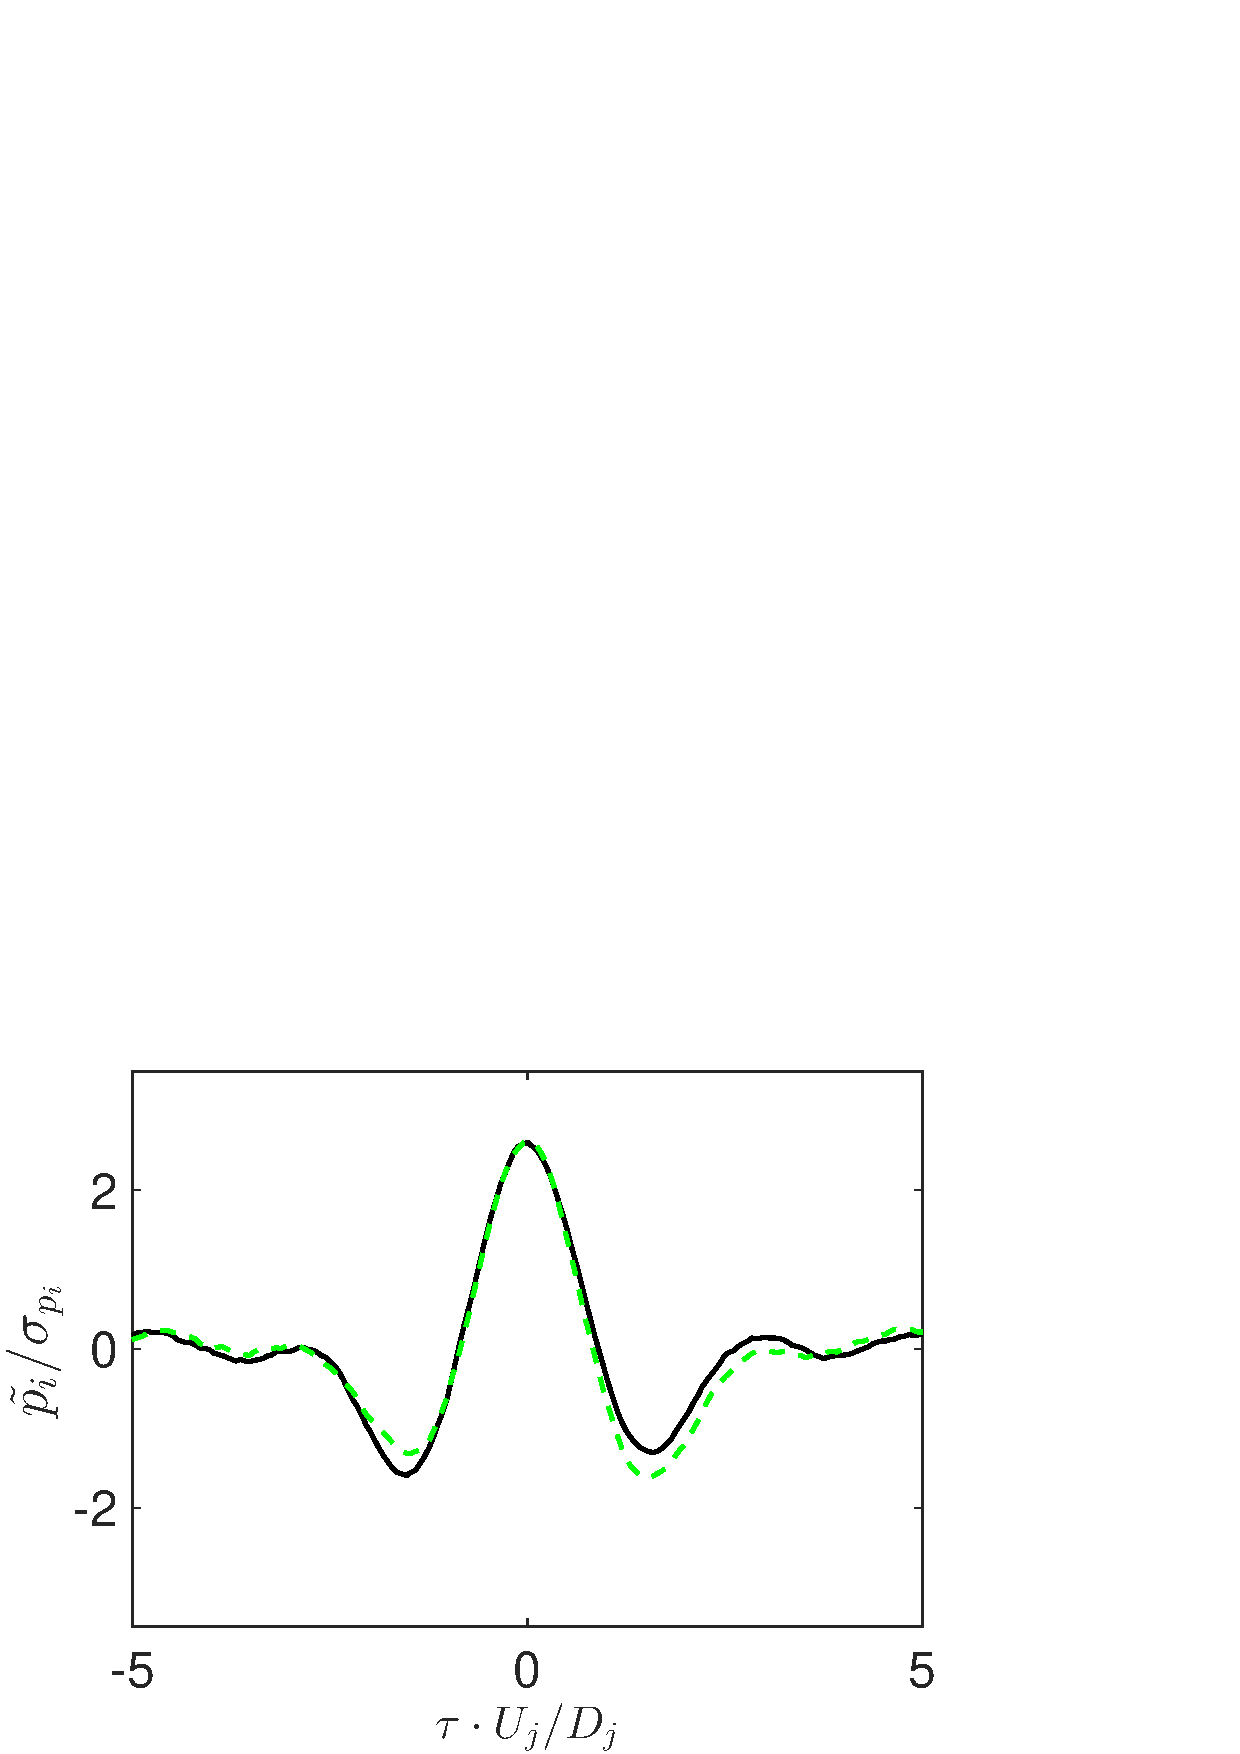
\includegraphics[width=0.45\linewidth]{Figures/compPeaks}
	\caption{Auto--conditioning signatures of the signal at $x/D = 3$} \label{fig:compPeaks}
\end{figure}
\fig{fig:compPeaks} presents the two subfigures for the different cases (negative/positive peaks) and a third subfigure to compare them.
\begin{itemize}
  \item $(a)$ conditional--average (\eq{eqn:ensembleAverage}) using only the negative peaks
  \item $(b)$ only the positive peaks
  \item a comparison between the two previous one ($(a)$ was inverted in order to compare it to $(b)$)
\end{itemize}
\fig{fig:compPeaks}c presents the resemblance between the signature of subfigures (a) and (b) on which the conditional--average was performed using only negative or positive peaks (it is important to understand that the differentiation is done by evaluating the value of each peak in the real domain and not in the LIM/wavelet domain). At this point, it is believed to be the result of the passage of two successive large scale turbulent--structures, in the zone where their interaction take place.
The formulation of the conditional--average was modified to take this observation into account and reformulated as follows:
\begin{equation} \label{eqn:condAvgSign}
\tilde{p}_{m}^n\left( W \right) = \left< p_{m} | P_{k} \right>_{\tilde{\tau}^n_{s}} = \frac{1}{N^n} \sum^{N^n}_{i = 1} sign\left( p_{n} \left( \tilde{t}_{i} \right) \right) p_{m} \left( \xi_{i} \right),
\end{equation}
$sign\left( p_{n} \left( \tilde{t}_{i} \right) \right)$ is introduced to take into account the sign of the peak in the real domain. This operation might be unnecessary for an experimental database (with a long time--series) but for a numerical database which is strongly limited in its time duration it improves the results obtained with the wavelet--conditioning.
The conditional--average using \eq{eqn:ensembleAverage} with all the peaks present (not presented here) is not relevant as additional proof for the separation between negative/positive peaks.
When the conditional--average is performed on a signal $p_{n}$ by using its own set of times ${\tilde{\tau}^n_{s}}$, making $n = m$; it becomes the auto--conditioning. If the conditional--average of a signal $p_{m}$ is done by using the set of times of a signal $p_{n}$, and so $n \neq m$; it is then called the cross--conditioning. The auto/cross--conditioning are presented in \fig{fig:condNcond}: the top is the auto--conditioning where the selection of $W$ is done in the reference signal $n$; and the bottom is the cross--conditioning of another signal $m$ where $W$ is centered around the times obtained with signal $n$. For more information about the wavelet--transform, see \cite{Farge1992}. The cross--conditioning is only presented in theory but no results with valuable meaning were obtained for this specific study.
\begin{figure}
	\centering
	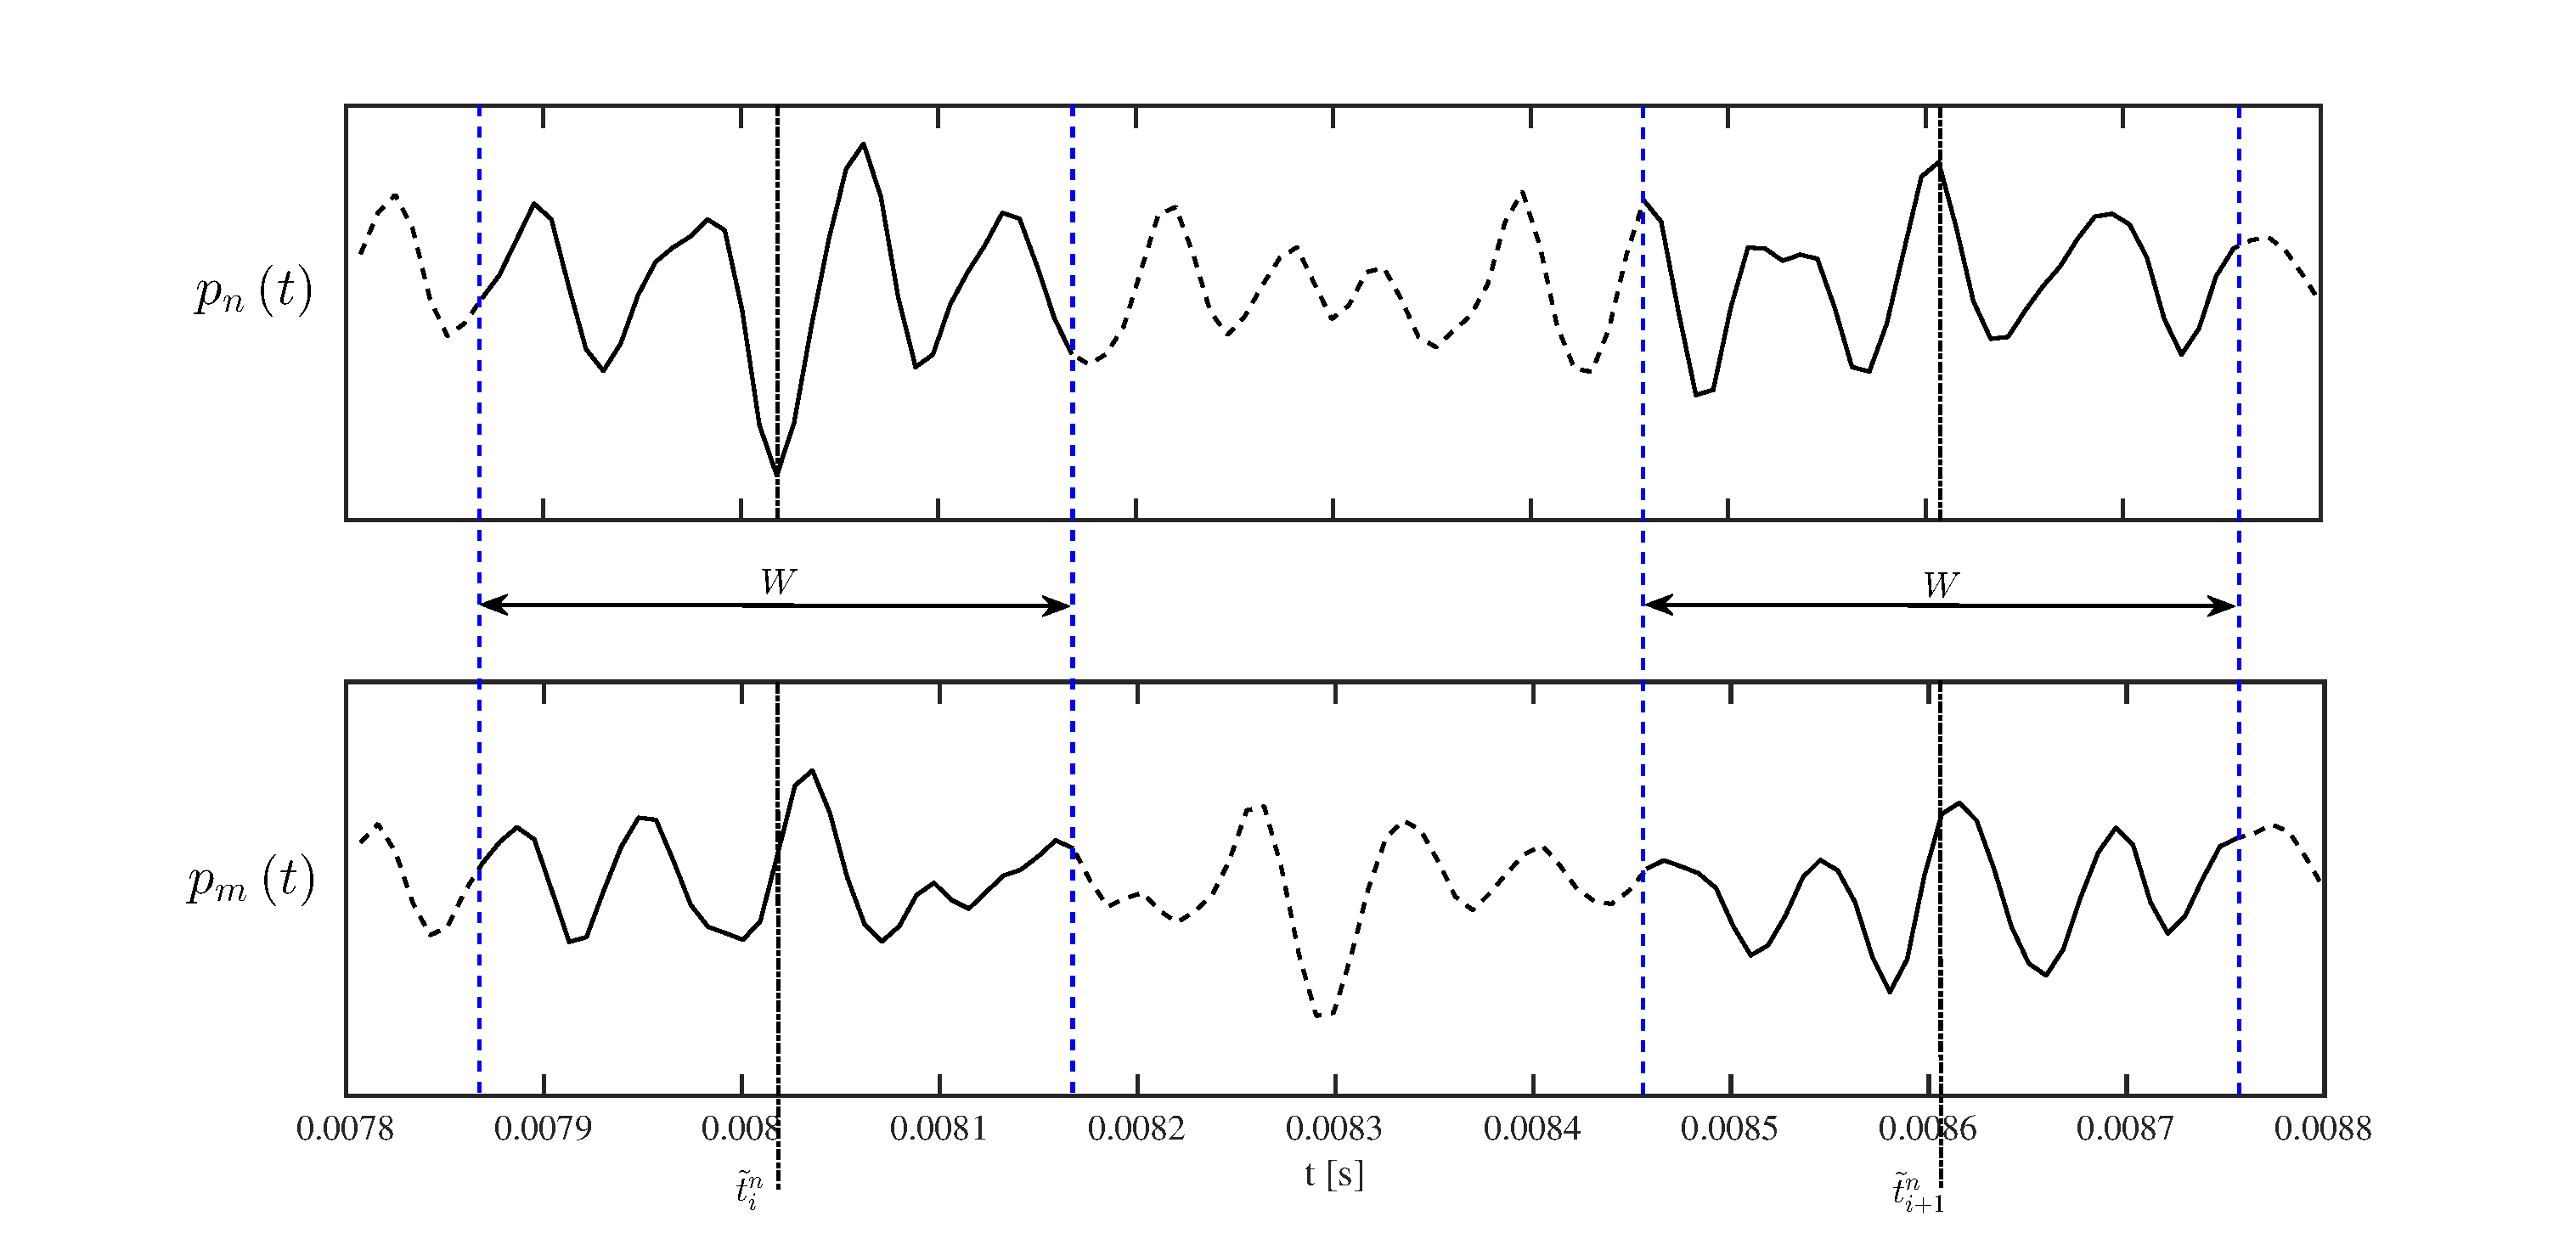
\includegraphics[width=1\textwidth]{Figures/condNcond.eps}
	\caption{\textit{Auto--conditioning of a signal $p_n(t)$ and cross--conditioning of a signal $p_n(t)$}}
	\label{fig:condNcond}
\end{figure}

For sake of brevity, only the results for four different cases, baseline and $S_t = 0.05, 0.25,$ and $0.35$, are presented. The following figure (\fig{fig:autoCondSt0p00}) represents the auto--conditioning of closest microphones array at $r/D = 1.2$ and for the microphones contained between $x/D=1$ and $x/D=14$. Here, only the positive peaks are used to perform the conditional--average. The reason will be explained later with a forced case. The results are non-dimensionalized by the local standard deviation. The first observation is that the energetic event detected using the wavelet--conditioning consists of a positive (or negative) central peak surrounded by two smaller lobs of the opposite sign. The local time--scale of the fluctuation grows as it is convected downstream. It is an expected result and can be reproduced using a simple auto--correlation at each axial position. The interests is to be able to appreciate the variation of the amplitude of the event according to its axial position. Up to $x/D=10$, the amplitude of the event is greater than the local standard deviation by at least twice. Then the fluctuation seems to get weaker and weaker as it is convected further downstream. 

\begin{figure}
	\centering
	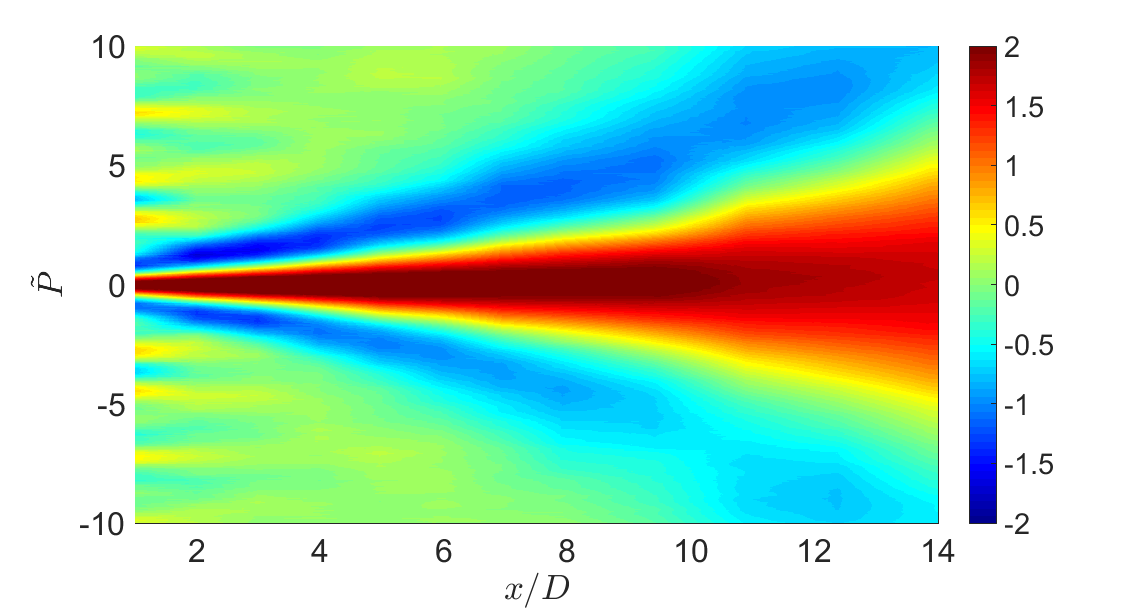
\includegraphics[width=1\textwidth]{Figures/conditioning/autoCondSt0p00.png}
	\caption{\textit{Auto--conditioning of a signal $p_n(t)$ and cross--conditioning of a signal $p_n(t)$}}
	\label{fig:autoCondSt0p00}
\end{figure}

The next figure \fig{fig:autoCondSt0p05} represents the auto--conditioning using the forced case at $S_t = 0.05$. The shape of the energetic event is different with compare to the previous case: it consists of a central peak, here positive, followed by a negative lob. The negative lob is at first of the same amplitude as the central peak and is becoming weaker as the event is convected further downstream. It is interesting to see that downstream, from around $x/D=8$, the energetic event shape of the excited case becomes more similar to the baseline, consisting of a central peak and surrounded by two lobs of the opposite sign. This is the reason of why the conditional--average is done using only the positive (or negative) peaks. The region in which the central peak start to strongly becomes weaker is closer to the nozzle exit, in this case around $x/D = 8$. 

\begin{figure}
	\centering
	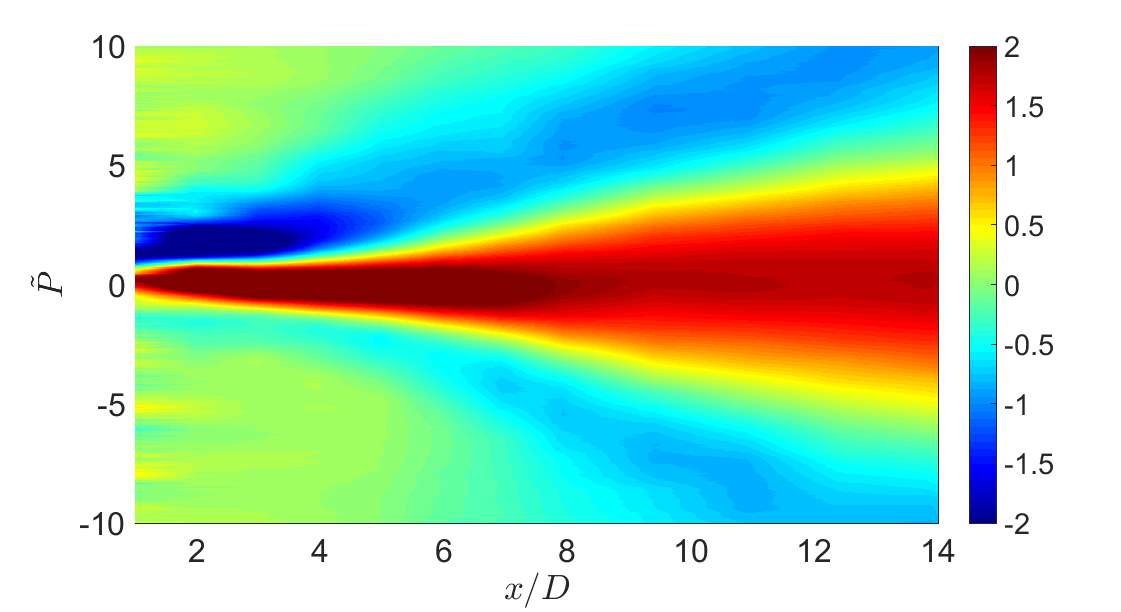
\includegraphics[width=1\textwidth]{Figures/conditioning/autoCondSt0p05.png}
	\caption{\textit{Auto--conditioning of a signal $p_n(t)$ and cross--conditioning of a signal $p_n(t)$}}
	\label{fig:autoCondSt0p05}
\end{figure}

The highest forcing cases are presented next. It can be observed from figures \fig{fig:autoCondSt0p25} and \fig{fig:autoCondSt0p35} that there are many similarities between these two cases. Using the same time scale of the two previous cases, it can be observed multiple energetic events on the same figure. For the case $S_t = 0.25$ case, the energetic event seems to be the same as $S_t = 0.05$. For the highest case it is more difficult to observe it as the time between two successive energetic events is really short and so two successive events are overlapping each other. 

\begin{figure}
	\centering
	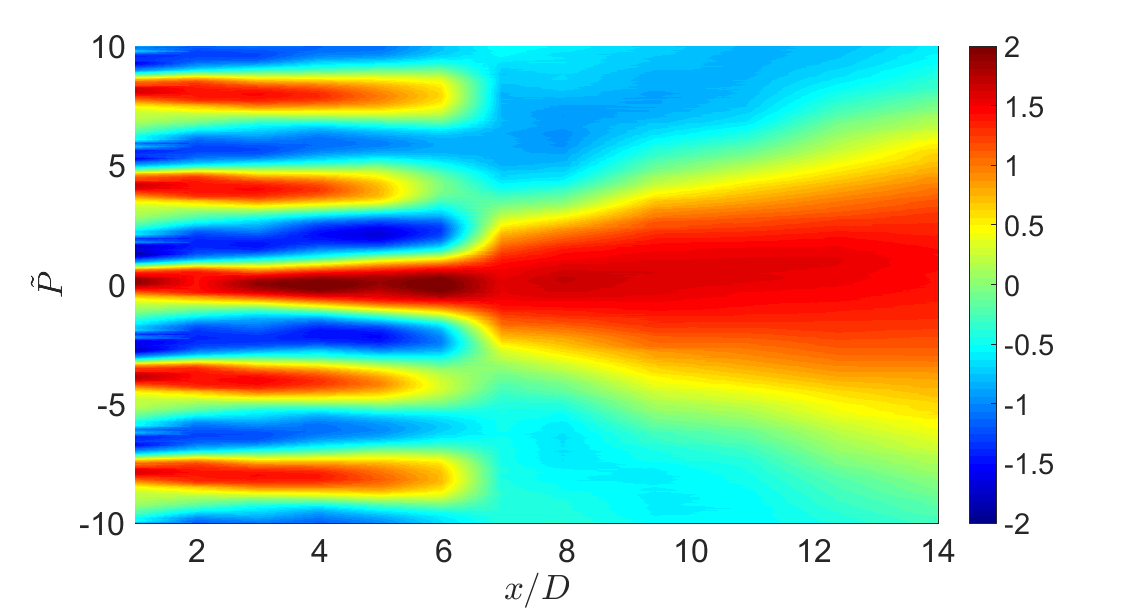
\includegraphics[width=1\textwidth]{Figures/conditioning/autoCondSt0p25.png}
	\caption{\textit{Auto--conditioning of a signal $p_n(t)$ and cross--conditioning of a signal $p_n(t)$}}
	\label{fig:autoCondSt0p25}
\end{figure}

\begin{figure}
	\centering
	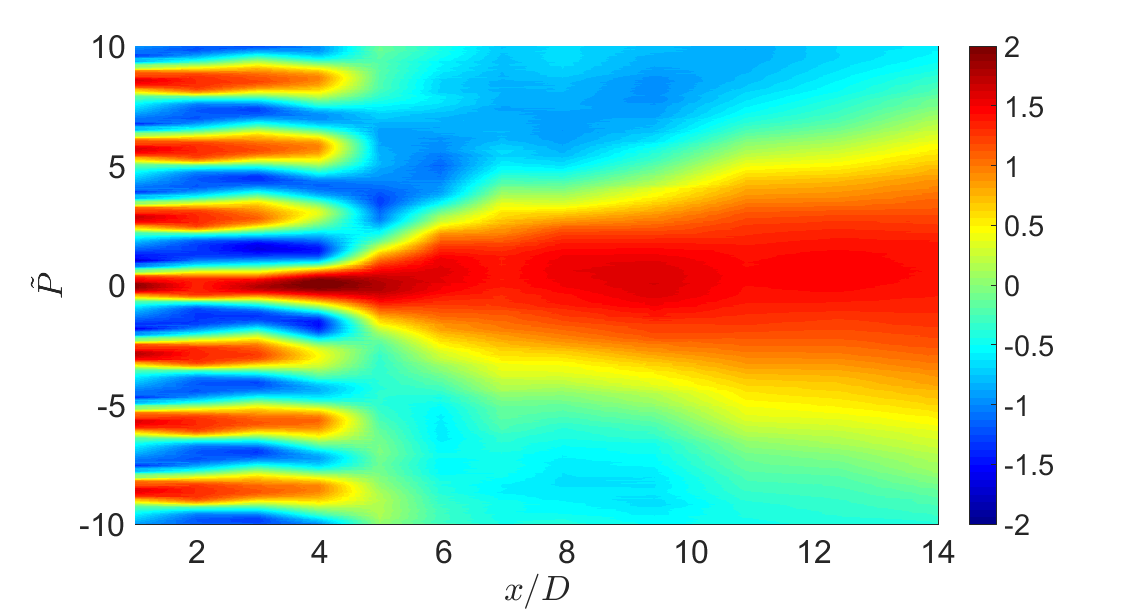
\includegraphics[width=1\textwidth]{Figures/conditioning/autoCondSt0p35.png}
	\caption{\textit{Auto--conditioning of a signal $p_n(t)$ and cross--conditioning of a signal $p_n(t)$}}
	\label{fig:autoCondSt0p35}
\end{figure}
The characteristic energetic--events of the forced cases are not similar in shape to the baseline, a central peak surrounded by two smaller of the opposite sign. It can be noted that the distance from the nozzle on which the excitation takes effect is becoming shorter as the excitation is higher: on figure \fig{fig:autoCondSt0p25} the excitation seems to maintain up to $x/D=6$ while on the following figure, \fig{fig:autoCondSt0p35}, it is up to $x/D=4$, shortened by around $2D$ with compare to the lowest case. 
%%%%%%%%%%%%%%%%%%%%%%%%
All the figure presented in this section are time--structures. It is possible to obtain spatial structures by doing the conditional average in space instead in time. To do so, 

\subsection{Identifying the Acoustic Source Region}
\label{sect:near_field_source_region}
Much of the difficulty in identifying the aeroacoustic source terms revolves around the dissimilar range of scales and fluctuation intensities of the turbulent eddies in the shear layer and the resulting radiated noise. 
Outside the jet shear layer, in the irrotational near-field of the jet, strong hydrodynamic pressure fluctuations associated directly with the passage of coherent structures in the shear layer and their resultant weak acoustic radiation coexist \citep{Arndt1997}. 
Beyond this, in the acoustic far-field, the hydrodynamic signature of the coherent structures is nonexistent owing to their strong exponential decay with radial distance.
Owing to this, identification of pure acoustic waves and their corresponding source events is problematic.
A decomposition of the pressure field into its constitutive hydrodynamic and acoustic components is therefore required. 
By identification and prediction of coherence nulls in the near field, \citet{Coiffet2006} showed that the full irrotational near-field consistent primarily as a linear superposition of its hydrodynamic and acoustic components, which lead subsequent researchers to propose linear filters to extract the individual components from the near-field pressure, with varying degrees of success. 

As discussed by \citet{Tinney2008}, in a transonic jet in which the large-scale structures are convecting subsonically with respect to the ambient speed of sound, a demarcation of the hydrodynamic and acoustic energy fields can be observed with phase velocity.
This is because the hydrodynamic pressure fluctuations will be aligned with the jet axis, and traveling subsonically. 
Acoustic pressure fluctuations will impinge on the linear microphone array at oblique angles, and therefore will appear as having either sonic or supersonic phase velocity, based on the source location. 
Therefore, a demarcaction between the hydrodynamic and acoustic energy components should be readily identifiable about the sonic wavenumber, $k_a = \omega / a_\infty$.
Decomposition of the irrotational near-field pressure is therefore straightforward in Fourier space.

However, there is also a great drawback associated with Fourier analysis: while it analyzes a given signal at a distinct frequency, local information for a given event is spread over all spectral coefficients. 
This is due to the fact that the basis functions used by the Fourier transform oscillate indefinitely. 
For a signal composed of completely random fluctuations this is not an issue, however it has become increasingly clear that the jet noise phenomenon is not a random process \citep{Kearney-Fischer2013}.
Transient events, such as intermittency or the spatial and temporal modulation of a wavepacket, have been shown to be important in the noise generation process. 
It was for this reason that a continuous spatio-temporal wavelet filter, based off of the work of \cite{Antoine2004} and \cite{Kikuchi2010}, was instead used in the current work to decompose the acoustic and hydrodynamic near-fields based on phase-velocity.
It has been shown that by using a temporally/spatially localized fluctuation as a basis, the wavelet transform compresses the information in a turbulent field much more efficiently (and accurately) than the Fourier transform \citep{Farge1992}.
A much more detailed explanation of the spatio-temporal wavelet transform, the justification for its use in decomposing the near-field pressure, and validation of the methodology using the current database can be found in \citet{Crawley2016}. 

By decomposing the irrotational near-field pressure, the relationship between the near- and far-field can be more easily elucidated. 
Two-point correlations were computed using both the full near-field and the acoustic near-field component, between each microphone in the near field and the far-field microphone at $30^\circ$; results can be found in \fig{fig:ch3_full_vs_partial_xcorr}. 
Examination in the spatio-temporal domain shows distinct regions of positive and negative correlation spanning several jet diameters and flow time scales.
The time lag, $\tau$, in the figures have been non-dimensionalized by the ambient speed of sound, $a_\infty$, and $R$, the distance from each near-field microphone to the far-field microphone (note that this results in an ordinate that is scaled separately along the abscissa, due to the dependence of the axial position on $R$).
\begin{figure}
	\centering
		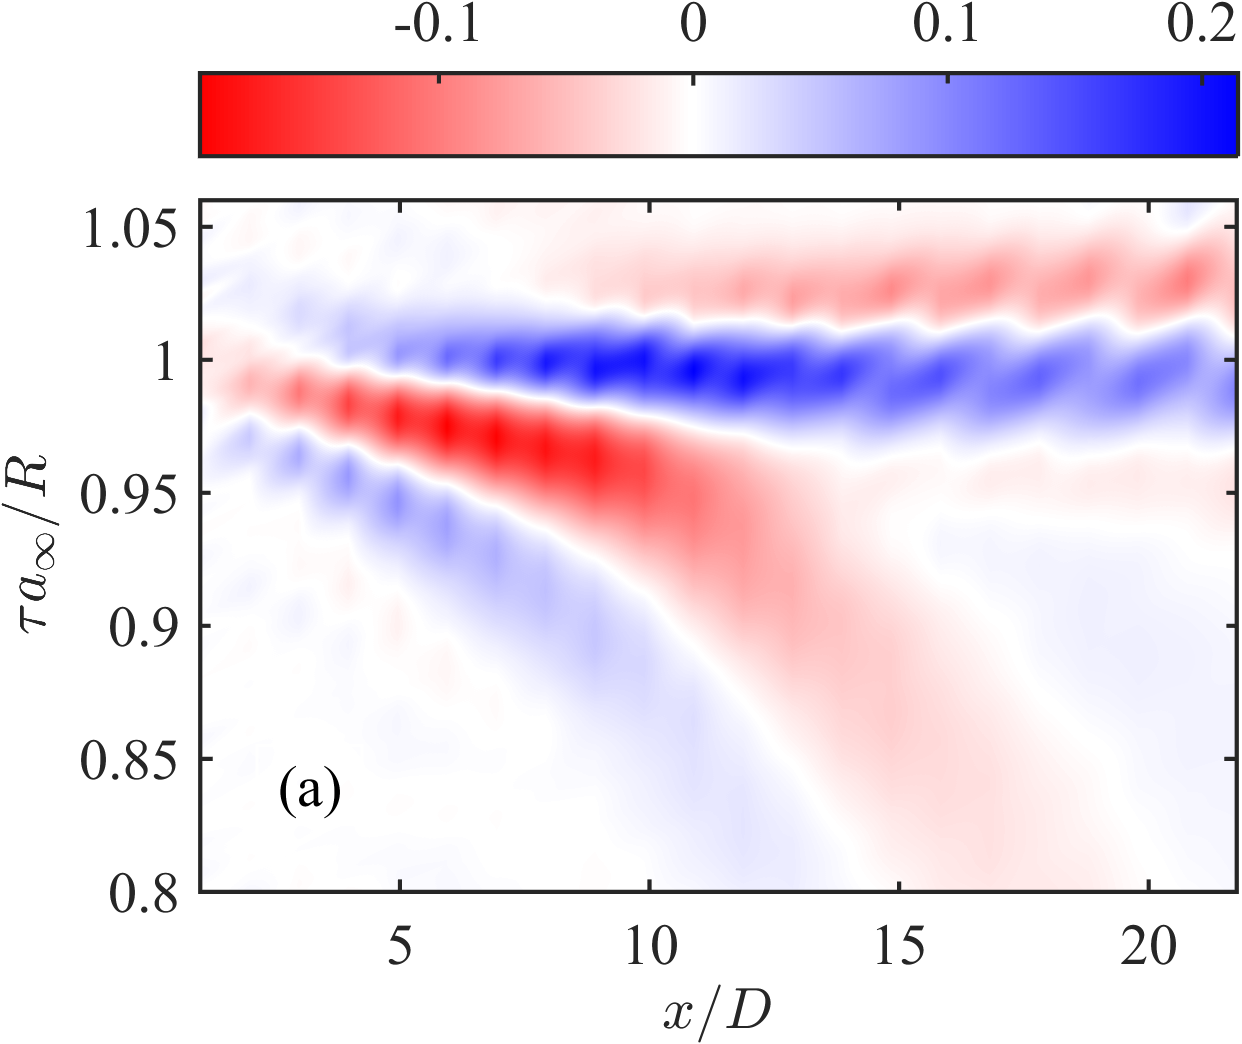
\includegraphics[width=0.475\linewidth]{Figures/sect_nearfield_fullxcorr.png}
		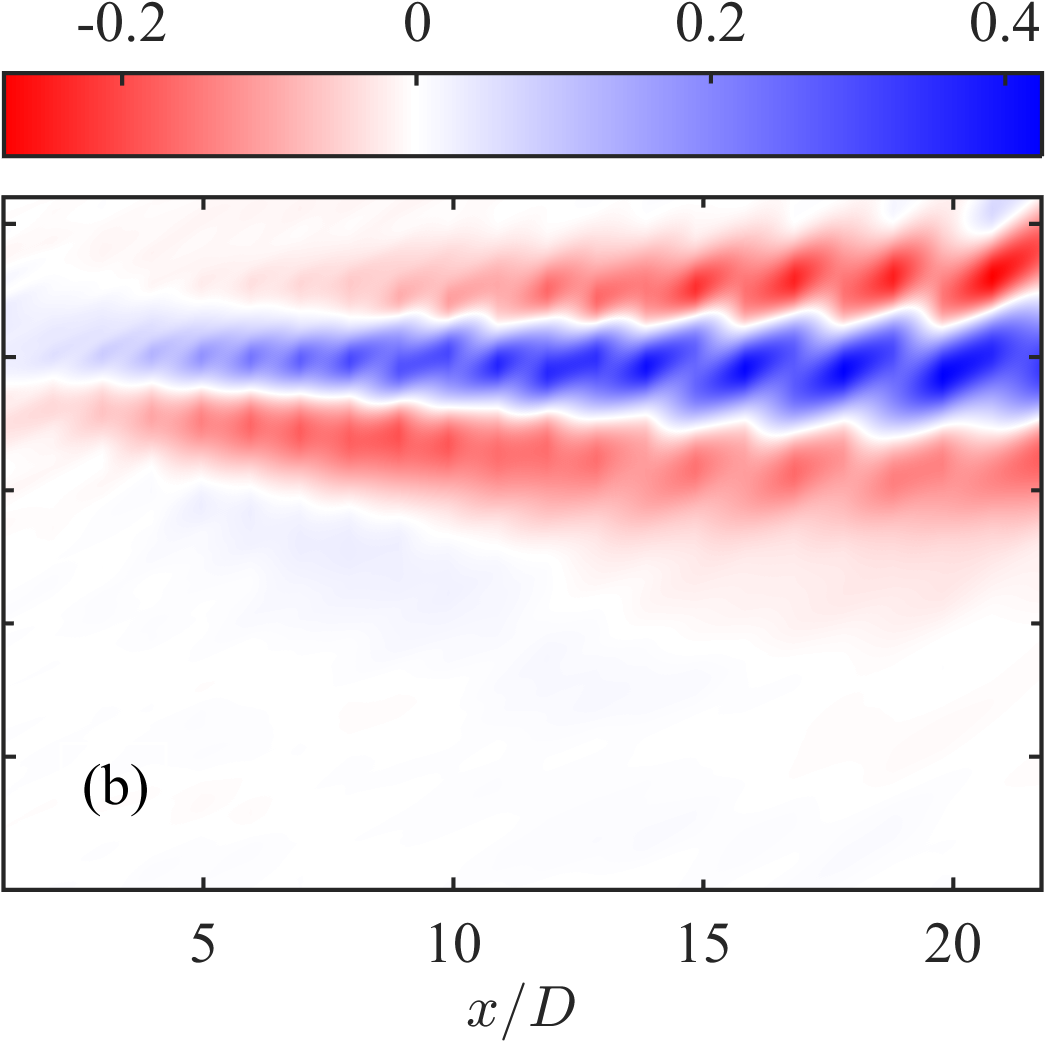
\includegraphics[width=0.401\linewidth]{Figures/sect_nearfield_acousticxcorr.png}
	\caption{Normalized two-point correlations for the natural jet between the near field and the far field at $30^\circ$ for the full near-field pressure (a) and the acoustic component only (b).}
	\label{fig:ch3_full_vs_partial_xcorr}
\end{figure}

Near the jet shear layer (\fig{fig:ch3_full_vs_partial_xcorr}a), four distinct correlation regions can be observed: two positive, two negative; one strong and one weak for each. 
The first correlation regions, the strong-negative and weak-positive, are noticeable beginning at the most upstream microphone and reach their peak values around $5 < x/D < 10$, decaying significantly beyond that.
The slopes of these regions indicate propagation velocities noticeably below the sonic velocity; in the upstream region, they roughly match with the measured convective velocity of the large-scale structures ($U_c \simeq 0.7 U_j$ as measured by two-point correlations between subsequent near-field microphones, see \citet{Crawley2015} for additional details) in the upstream region of the jet, and slowly decelerate downstream.
Similar behavior was observed by \citet{Bogey2007}, who noted that two-point correlations between the flow-field and acoustic near-field in a simulated jet produced strong positive correlation regions which peaked at the end of the potential core and which followed the convection of the large-scale structures.
Conversely, the strong-positive and weak-negative correlation regions exhibit propagation velocities that match well with the ambient speed of sound. 
The distinctly different propagation velocities and of the two pairs of correlation regions indicate that these correspond to different physical phenomena.
The strong-negative and weak-positive correlation regions observed near the jet shear layer are associated with the large-scale structures themselves, rather than acoustic phenomena. 
This relationship becomes even more clear when just the acoustic component of the near-field is considered, rather than the full irrotational near-field. 
Gone entirely now are the correlation regions with subsonic propagation velocities (\fig{fig:ch3_full_vs_partial_xcorr}b), and instead, a single positive correlation region corresponding to sonically-propagating waves exists over the entire domain. 

The correlations of the decomposed near-field can be used to identify the acoustic source region, at least in a rough sense, by comparing the time lag at which the greatest correlation is achieved against expected times-of-arrival for different propagation paths.
A schematic of these propagation paths is provided in \fig{fig:ch3_ToA}.
The first expected time of arrival, $\tau_a$, corresponds to the expected time lag for an acoustic wave traveling directly from the noise source to the near-field microphone and on to the far-field microphone and hence, the noise source region lies along the axis created by the near-field and far-field microphones.
Another expected time-of-arrival can be constructed by assuming the source region is stationary in space; from simple geometric considerations of the distance from the assumed source region to the near-field and far-field microphones, the time lag, $\tau_s$, between the arrival of an acoustic wave at both microphones can be computed.
The stationary source region is of course not known \textit{a priori}, but is set by the author subsequent to the computation of the two-point correlations.

For simplicity, density and convection effects on the acoustic wave as it travels through the jet shear layer have been neglected in this analysis. 
By necessity, it has been assumed that the acoustic radiation in the jet is dominated by $m = 0$ azimuthal Fourier mode (the near-field and far-field microphone arrays are not at the same azimuthal angle with respect to the nozzle). 
This assumption is easily justified in the excited jets, where the actuators have been fired in phase. 
While the near-field pressure and acoustic radiation towards aft polar angles in a natural, high Reynolds number jet is a combination of numerous azimuthal Fourier modes, previous researchers have found these fields to be dominated by the axisymmetric mode \citep{Arndt1997,Hall2006,Koenig2013,Juve1979}.
\begin{figure}
	\centering
	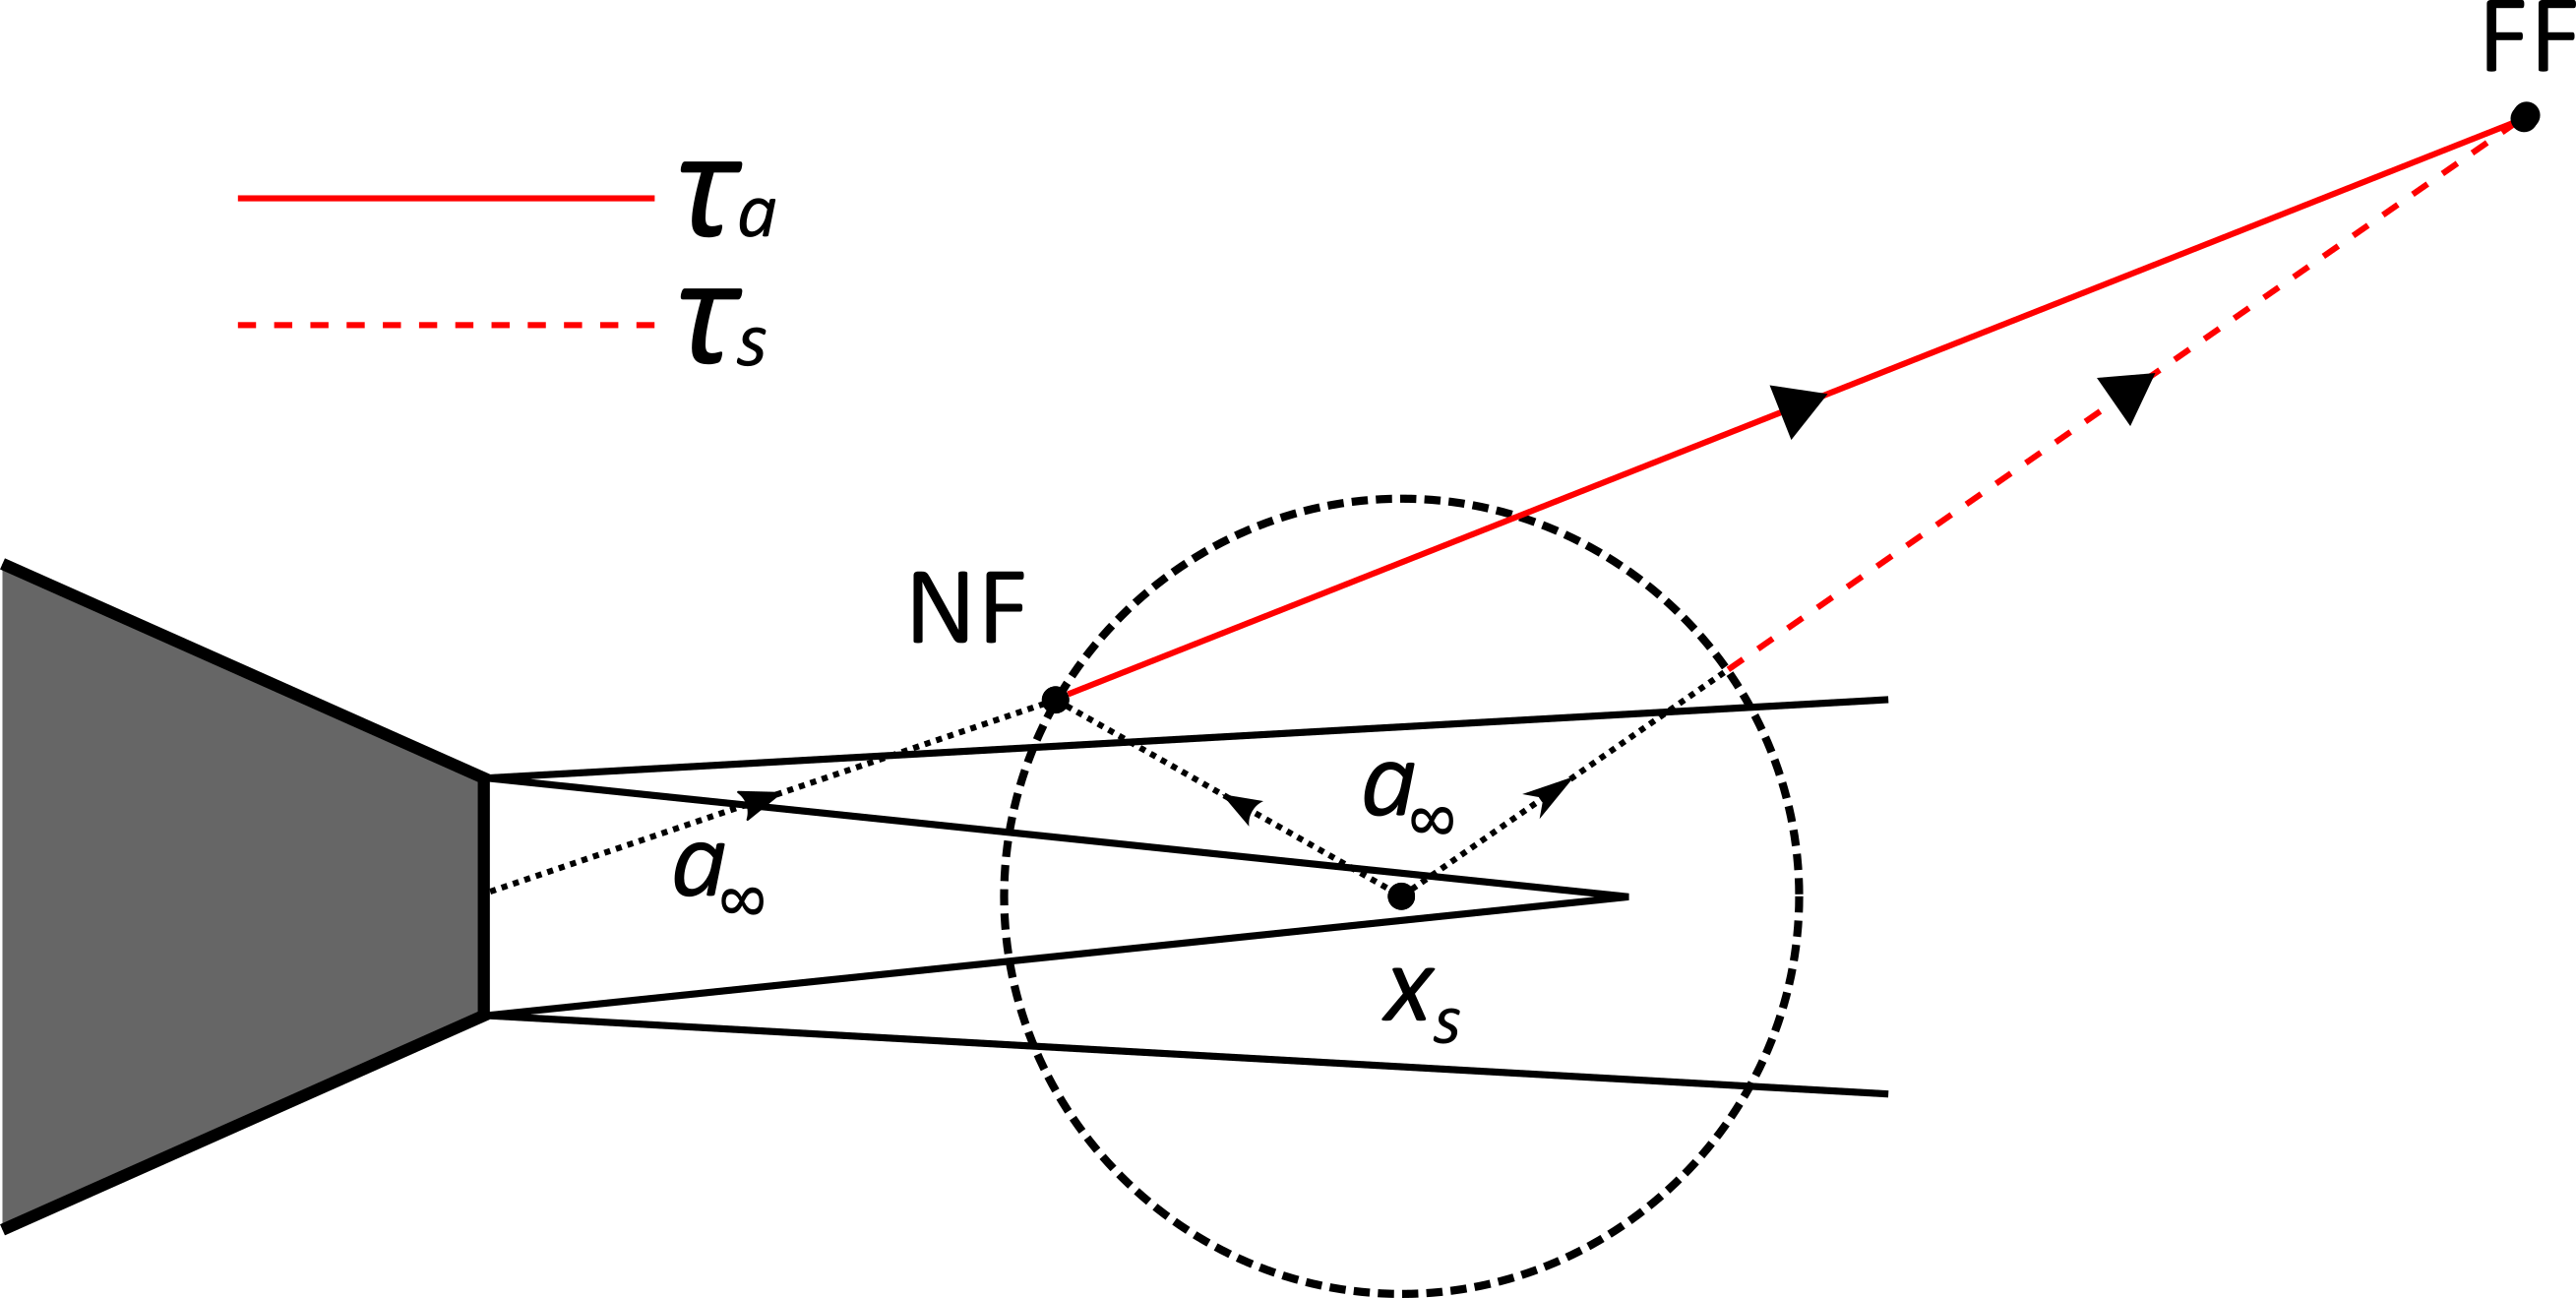
\includegraphics[width=3in]{Figures/ToA_tau.png}
	\caption{Expected times of arrival for on-axis acoustic propagation, $\tau_a$, and off-axis acoustic propagation, $\tau_s$ from a stationary source region centered at $x_s$.}
	\label{fig:ch3_ToA}
\end{figure}

Here, the acoustic source region was assumed to be located at $x_s /D = 4$, which is just upstream of the end of the potential core in the unforced jet. 
(Please note that this analysis is not meant to imply that the source region is located at a specific, fixed point – it is merely a convenient way of understanding the propagation paths.)
Similar behavior is observed between the natural jet and the excited cases in \fig{fig:ch3_xcorrOA}; note that due to numerical discrepancies at the domain boundaries (see \citet{Torrence1998} for a discussion of the `cone of influence' of wavelet coefficients and the effect thereof), the correlation values have been truncated at the most upstream and downstream microphones.
For the impulsively-excited jet, nearly identical correlation regions are observed between the excited and natural jet; in the periodically-excited jet continuous oscillations occur throughout time due to the similarity of continuously-generated large-scale structures and resultant acoustic radiation.
In the upstream region of the jet, the peaks of the positive correlation region match $\tau_a$ nearly exactly. 
In the downstream region, $\tau_a$ begins to increasingly over-predict the time lag for the maximum correlation. 
On the other hand, $\tau_s$ tracks the time lags for the peak correlation consistently over the downstream region, but not the upstream region. 
The results found here appear to indicate that the dominant acoustic radiation reaching the far-field aft angles is being generated over an extended region of the jet mixing layer, roughly $x/D \leq 4$, which is just upstream of the time-averaged end of the potential core in the natural jet.
This is not too dissimilar from the findings of other researchers, who have suggested that the acoustic source region lies just \textit{downstream} of the end of the potential core \citep{Hileman2005}.
It should be clarified here though, that the interpretation of these results is not meant to suggest that only trivial levels of noise are generated outside of this apparent noise source region, just that the dominant radiation is produced in this region in a time-averaged sense.
\begin{figure}
	\centering
	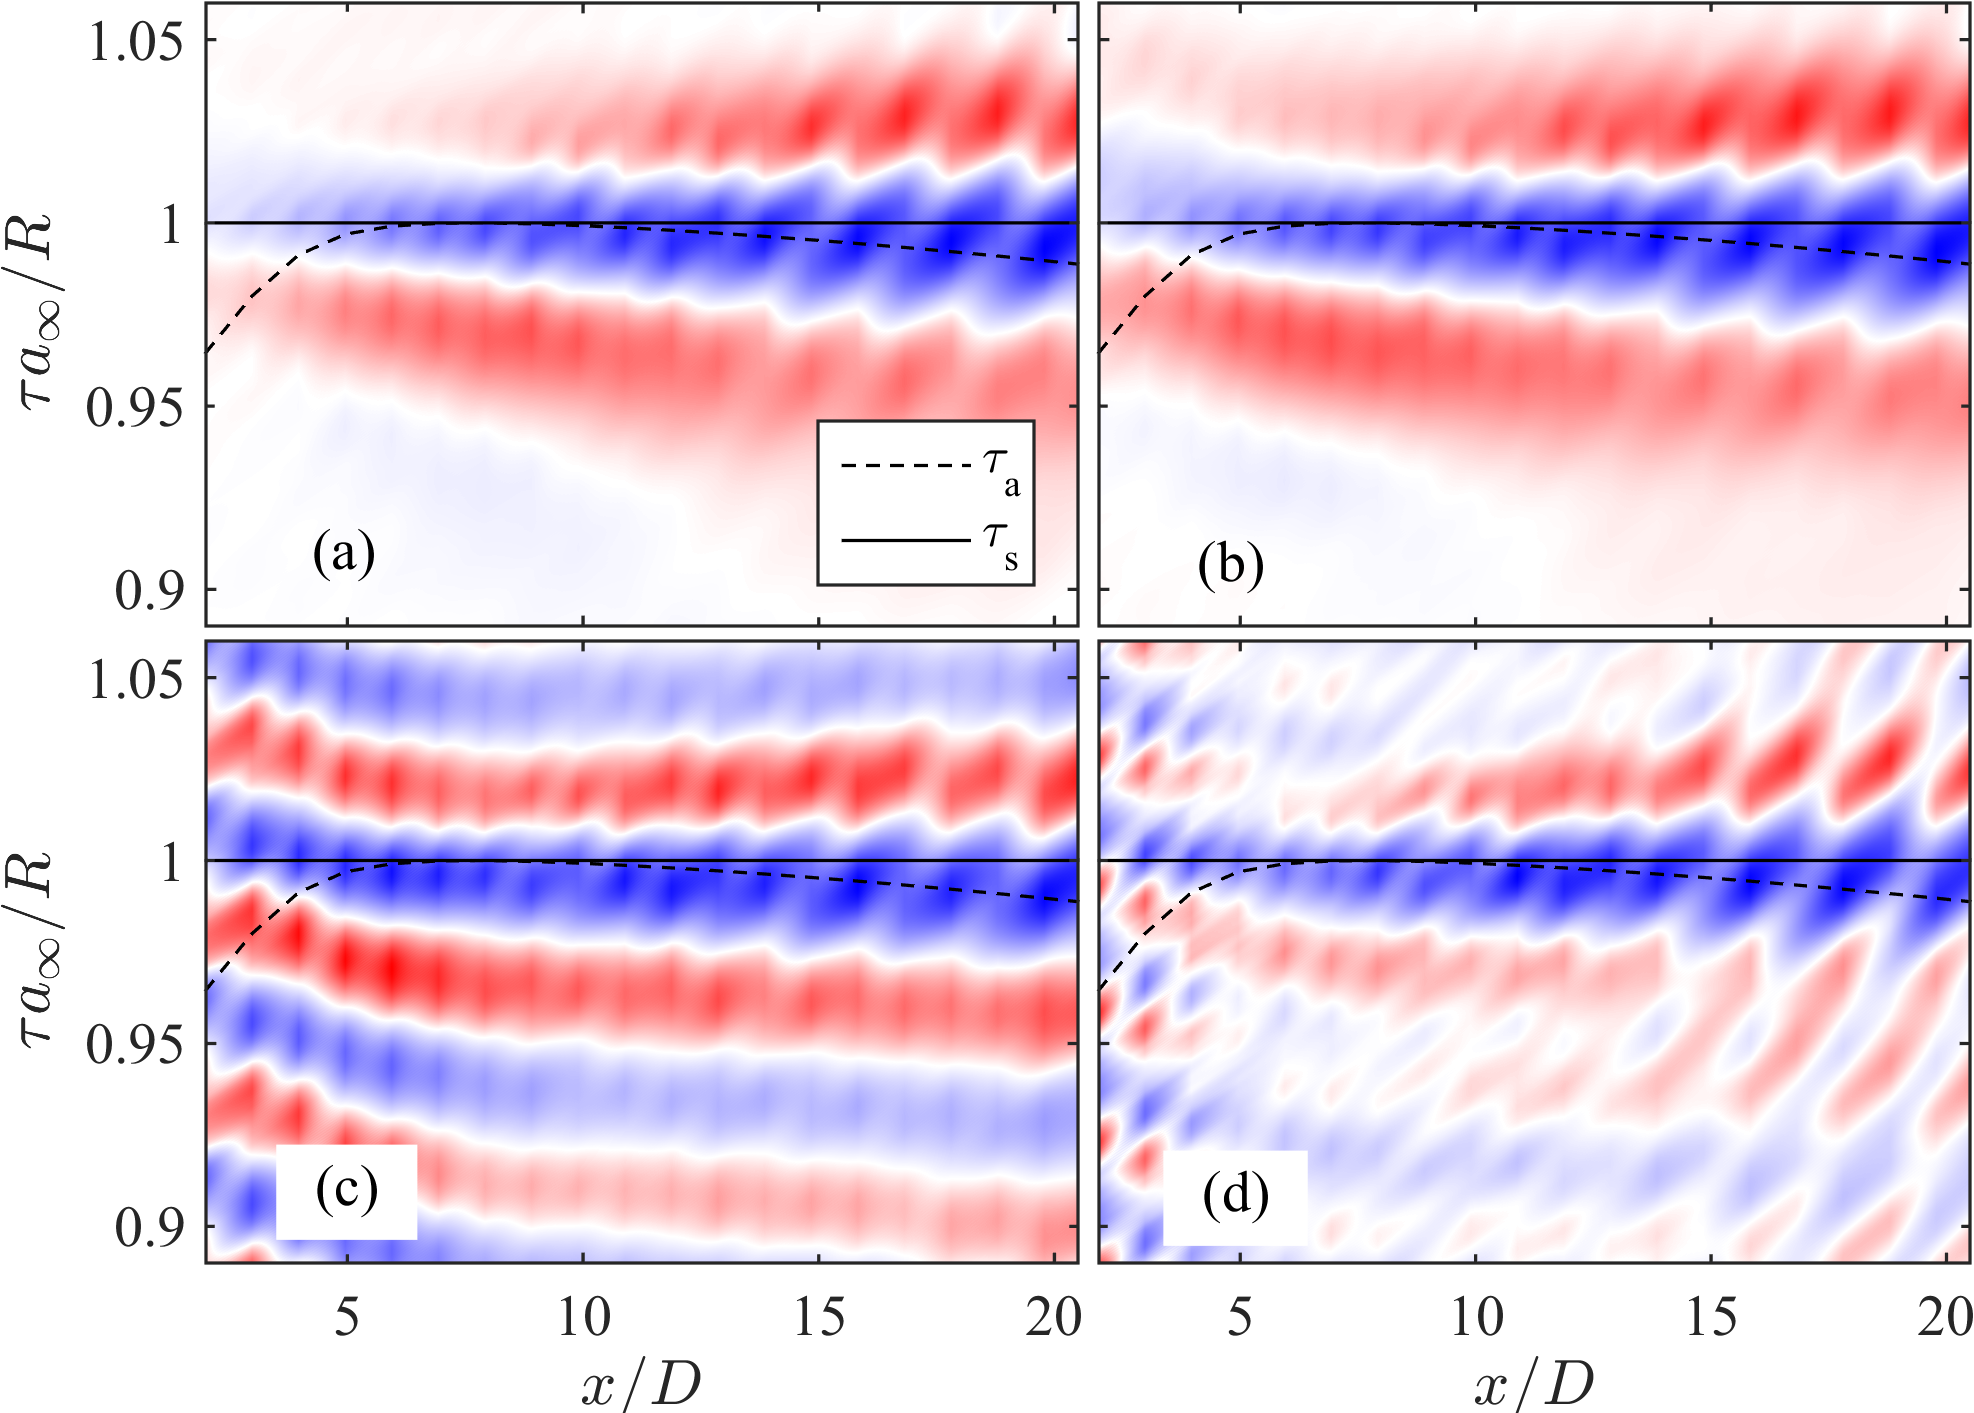
\includegraphics[width=\linewidth]{Figures/sect_nearfield_ffxcorr.png}
	\caption{Normalized two-point correlations between the acoustic component of the near field and the far field at $30^\circ$ for microphone array position starting at $x/D = 1, r/D = 1.2$ for the natural jet (a), $St_{DF} = 0.05$ (b), $St_{DF} = 0.25$ (c) and $St_{DF} = 0.35$ (d).}
	\label{fig:ch3_xcorrOA}
\end{figure}

However, these results should not be interpreted as indicating that the source mechanisms are necessarily consistent for all excitation frequencies. 
For the lower-frequency periodic excitation ($St_{DF} \leq 0.25$), the consistency in the far-field response (\fig{fig:ch3_farfield_linear}) coupled with the consistency in the apparent source region is suggestive of a consistent dominant source mechanism.
In contrast, the inconsistency in the far-field response for the higher-frequency periodic excitation ($St_{DF} \geq 0.35$, \fig{fig:ch3_farfield_nonlinear}) is suggestive of a change in the dominant source mechanism, just one that is associated with the vortex dynamics in the jet shear layer upstream of the end of the potential core.
It should also be noted that the peak correlation values between the acoustic near-field and the far-field are significantly lower (though certainly non-negligible) in the periodic excitation cases, suggesting a decaying coherence in the source mechanisms at these frequencies.
From the current results alone, the significance of this estimated source region is not entirely clear.
In \sect{sect:velocity} the time-resolved velocity field will be explored in detail to better elucidate the structure dynamics, with a particular focus on the region just upstream of the end of the potential core.

The authors would like to make a special note here, concerning the discrepancy between the results presented in \fig{fig:ch3_xcorrOA} and those presented previously in \citet{Crawley2015}.
In that paper, the more simple Fourier filter was used to decompose the irrotational near-field; processing artifacts were noted and a parametric study was attempted to minimize their impact.
In the resulting two-point correlations of the decomposed acoustic field, a shift in the apparent source region was noted to coincide with the shift of the peak pressure fluctuations measured just outside the shear layer (higher frequency excitation cases saturating further upstream near the nozzle exit).
Because this behavior was observed across the entire range of filter parameters used, it was assumed to be representative of the true physical behavior and not a numerical artifact.
Of course, this assumption precludes the possibility that \textit{the entire parameter space produced similar numerical artifacts}. 
As discussed more thoroughly in \citet{Crawley2016}, the Fourier filter has a tendency to allow energy leakage from the hydrodynamic field into the acoustic, particularly at low frequencies. 
Since it has already been observed that the hydrodynamic signature of the large-scale structures can linearly correlate to the acoustic emission, a potential consequence of this leakage is correlation regions which instead point to the region of high hydrodynamic energy - i.e. the saturation point of the near-field pressure fluctuations.
The analysis found of \citet{Crawley2016} demonstrated that wavelet filter is far more robust to energy leakage and numerical artifacts, and as such the authors is inclined to lend more credence to the results presented herein. 
\section{Vortex Dynamics in a Turbulent Mixing Layer}
\label{sect:velocity}
Analysis of the evolution, interaction, and disintegration of the large-scale structures, and ultimately the noise generated thereby, is greatly simplified by the acquisition of time-resolved flow-field measurements.
Furthermore, as will be explained in \sect{sect:source}, computation of the aeroacoustic source field from a simplified acoustic analogy will require time-resolved flow-field data.
Unfortunately, directly acquiring time-resolved velocity fields for the jet currently under study is simply not possible due to the combination of a large domain of interest ($0 \leq x/D \lesssim 12, 0 \leq r/D \lesssim 3$) and high characteristic frequencies on the order of tens of kHz.
Full-field, high-fidelity measurement techniques capable of this required repetition rate simply do not exist at present.
An indirect method is therefore required in order to estimate the evolution of the large-scale structures, in a reduced-order sense.

Phase-locking of a data acquisition system to a reference signal (such as an actuator or a naturally occurring resonance tone) is a common experimental technique, and was initially considered for the present work.
However, sample analysis performed using a numerical database indicated that a very high temporal resolution was required in order to accurately compute fluctuation rates in the dilatation field (the relevance of which will become more apparent in the following section).
At moderate to high excitation frequencies, this was feasible, though potentially tedious (for example, $\sim$16 phases were estimated as necessary at $St_{DF} =0.25$).
At $St_{DF} =0.05$ however, this would require roughly \textit{forty} phases (the significant dead time between actuations means that it is not necessary to acquire the entire range of phases from $0$ to $2\pi$, but this is small consolation).
Clearly, a more efficient data acquisition method is needed.

\subsection{Stochastic Estimation}
The current work borrows heavily from the methodology of \citet{Tinney2008b} and \citet{Sinha2010} in order to estimate the two-component time-resolved velocity field on a streamwise slice of the jet.
The computational methodology by which the stochastic estimation is performed has been modified, however.
Complementary stochastic estimation is used, due to its significantly lower computational cost as well as theorized improvement in accuracy \citep{Bonnet1994}.
The estimated velocity fields produced by LSE were projected onto the POD eigenfunctions (computed from the random, non-time-resolved velocity fields) to produce an estimate of the time-dependent POD coefficients, which can then be used to reconstruct low-order representations of the estimated random velocity field.
Multiple time delays are incorporated, as this has been found to significantly improve the accuracy of the reconstructions for many flow regimes \citep{Ewing1997,Tinney2006,Tinney2008b,Durgesh2010}.
Instead of performing the stochastic estimation using either linear or higher-order cross-correlations (or cross-spectra), the conditional mapping between the near-field pressure and the POD modal coefficients will be generated by an artificial neural network (ANN).
ANNs were chosen over the more traditional cross-correlations due to their simplicity compared to high-order methods as well as their demonstrated ability to model nonlinear processes in turbulent flows \citep{Lasagna2015}.

A feedforward network structure was used in the current work; comprised of an input layer, to which near-field pressure traces were supplied, a single hidden layer containing 32 neurons, and an output layer which produced estimates of the time-varying POD coefficients. 
The hidden and output layers were fully connected, and the modified logistic function (hyperbolic tangent) was used as the activation function.
The pressure traces were centered around the acquisition of a PIV image group, and was downsampled to 100 kHz in order to approximate the frequency response of the microphones.
The record time supplied for each training block was $\pm 2.56$ milliseconds; this was determined by estimating the time delay for a large-scale structure to convect through the experimental domain (the convective velocity of the large-scale structures was conservatively estimated as $U_c \simeq 0.5 U_j$).


POD modes and time-varying coefficients were computed from the velocity fields using the method of snapshots \citep{Sirovich1987}; the kernel was defined as the two-component turbulent kinetic energy.
The instantaneous velocity fields were not preprocessed prior to the decomposition (that is, missing or spurious vectors were not replaced or interpolated).
As experimental noise in the velocity fields will be completely uncorrelated to the near-field measurements, it will be filtered out by the stochastic estimation and hence preprocessing is unnecessary.
In this work, the coefficients for every POD mode were estimated, rather than just the most energetic modes, for two reasons.
First, it is not guaranteed that an individual POD mode corresponds to a physically distinct turbulent flow structure or event - an event may be broken up into multiple POD modes of varying energy levels.
Secondly, the most energetic POD mode is not necessarily the most relevant mode for the acoustic generation process (see \citet{Jordan2007} for a modification to the standard POD kernel in order to mitigate this issue).
The second issue is in fact not unique to the field of aeroacoustics but vexes turbulence research in general, where highly relevant dynamical processes may contain little energy \citep{Noack2008}; this has lead researchers to propose alternative methods for extracting dynamical features of turbulent flows \citep{Schmid2010}.
Even though the network is estimating even the least-energetic modes, the current method is far more computationally efficient than directly estimating the velocity fields themselves.
By encoding spatial correlations in the POD expansion coefficients, estimation of the $N$ snapshots of $M \times K$ spatial locations has been reduced from a minimization problem of $N$ vectors of $2MK$ to one of $N$ vectors of $N$.
For the current experimental database, this means the system has been reduced from $290,508 \times 1500$ to $1500 \times 1500$.
The neural network now only needs to identify the temporal correlations between the pressure field and the individual POD coefficients; it does not need to learn the spatial correlations.

Learning was accomplished via the standard backpropagation method \citep{Haykin1994}, which approximates the error surface of the cost function using first-order derivatives; the error `propagates' backwards from the output neurons to the hidden neurons and the synaptic weights at each neuron are updated to identify the (hopefully, global) minimum of the cost function using gradient descent.
The cost function was defined as the mean-squared-error between the predicted and measured expansion coefficients for a given PIV image group.
Training of the network was performed using the roughly 1500 ensemble pressure-velocity blocks of data (a few PIV images in each set had to be discarded due to laser misfires); synaptic weights were updated based on the average of all blocks (batch processing) using a constant learning rate.
A well-known issue with the gradient descent optimization method is that it has a tendency to get trapped in local minima and fails to converge to the global minimum.
Therefore, sample results were also calculated using a much different learning algorithm: adaptive particle swarm optimization.
Details will not be presented here however, as the results were found to not differ substantially from those produced by the backpropagation algorithm (while requiring significantly higher computational resources).


\subsection{Large-Scale Structure Disintegration}
\citet{Hileman2005} investigated the evolution and interactions of large-scale structures and ultimately how these relate to the noise generation process in a supersonic, ideally-expanded jet by combining time-resolved flow visualizations with a three-dimensional microphone array.
Their results showed that the dominant noise was being generated near the end of the potential core, in the region where the shear layers merged.
Large-amplitude, highly-intermittent acoustic events were found to be associated with a fluctuation in the length of the potential core, which the authors ultimately speculated was related to the passage and finally the rapid disintegration of large-scale coherent structures just downstream of the end of the potential core.
The results of ??? also indicated that the region upstream of the end of the potential core was responsible for the dominant acoustic generation in a subsonic jet, at least to low angles with respect to the jet axis.
The dynamics of the large-scale structures in this region, namely the structure disintegration, are therefore of particular concern to the current work.

Vortex identification was performed by computing the swirling strength at each instance in the estimated velocity field; details and justification for this method can be found in \citet{Adrian2000}.
The evolution of the impulsively excited ($St_{DF} = 0.05$) vortex ring has been tracked in \fig{fig:ch4_impulse_structure_disintegration}.
For ease of visualization, a two-dimensional, five-point boxcar filter was applied to the estimated velocity fields prior to computing the swirling strength, and the results have been phase-averaged based on the recorded LAFPA trigger signal over roughly 30 excitation periods.
Lastly, a solid red line has been overlain to approximately match the convective velocity of the structures.
Only a select number of phases are shown here, as a significant amount of dead time between excitations occurs due to the mismatch in the spatial and temporal characteristic frequencies of the large-scale structures.
\begin{figure}
	\centering
	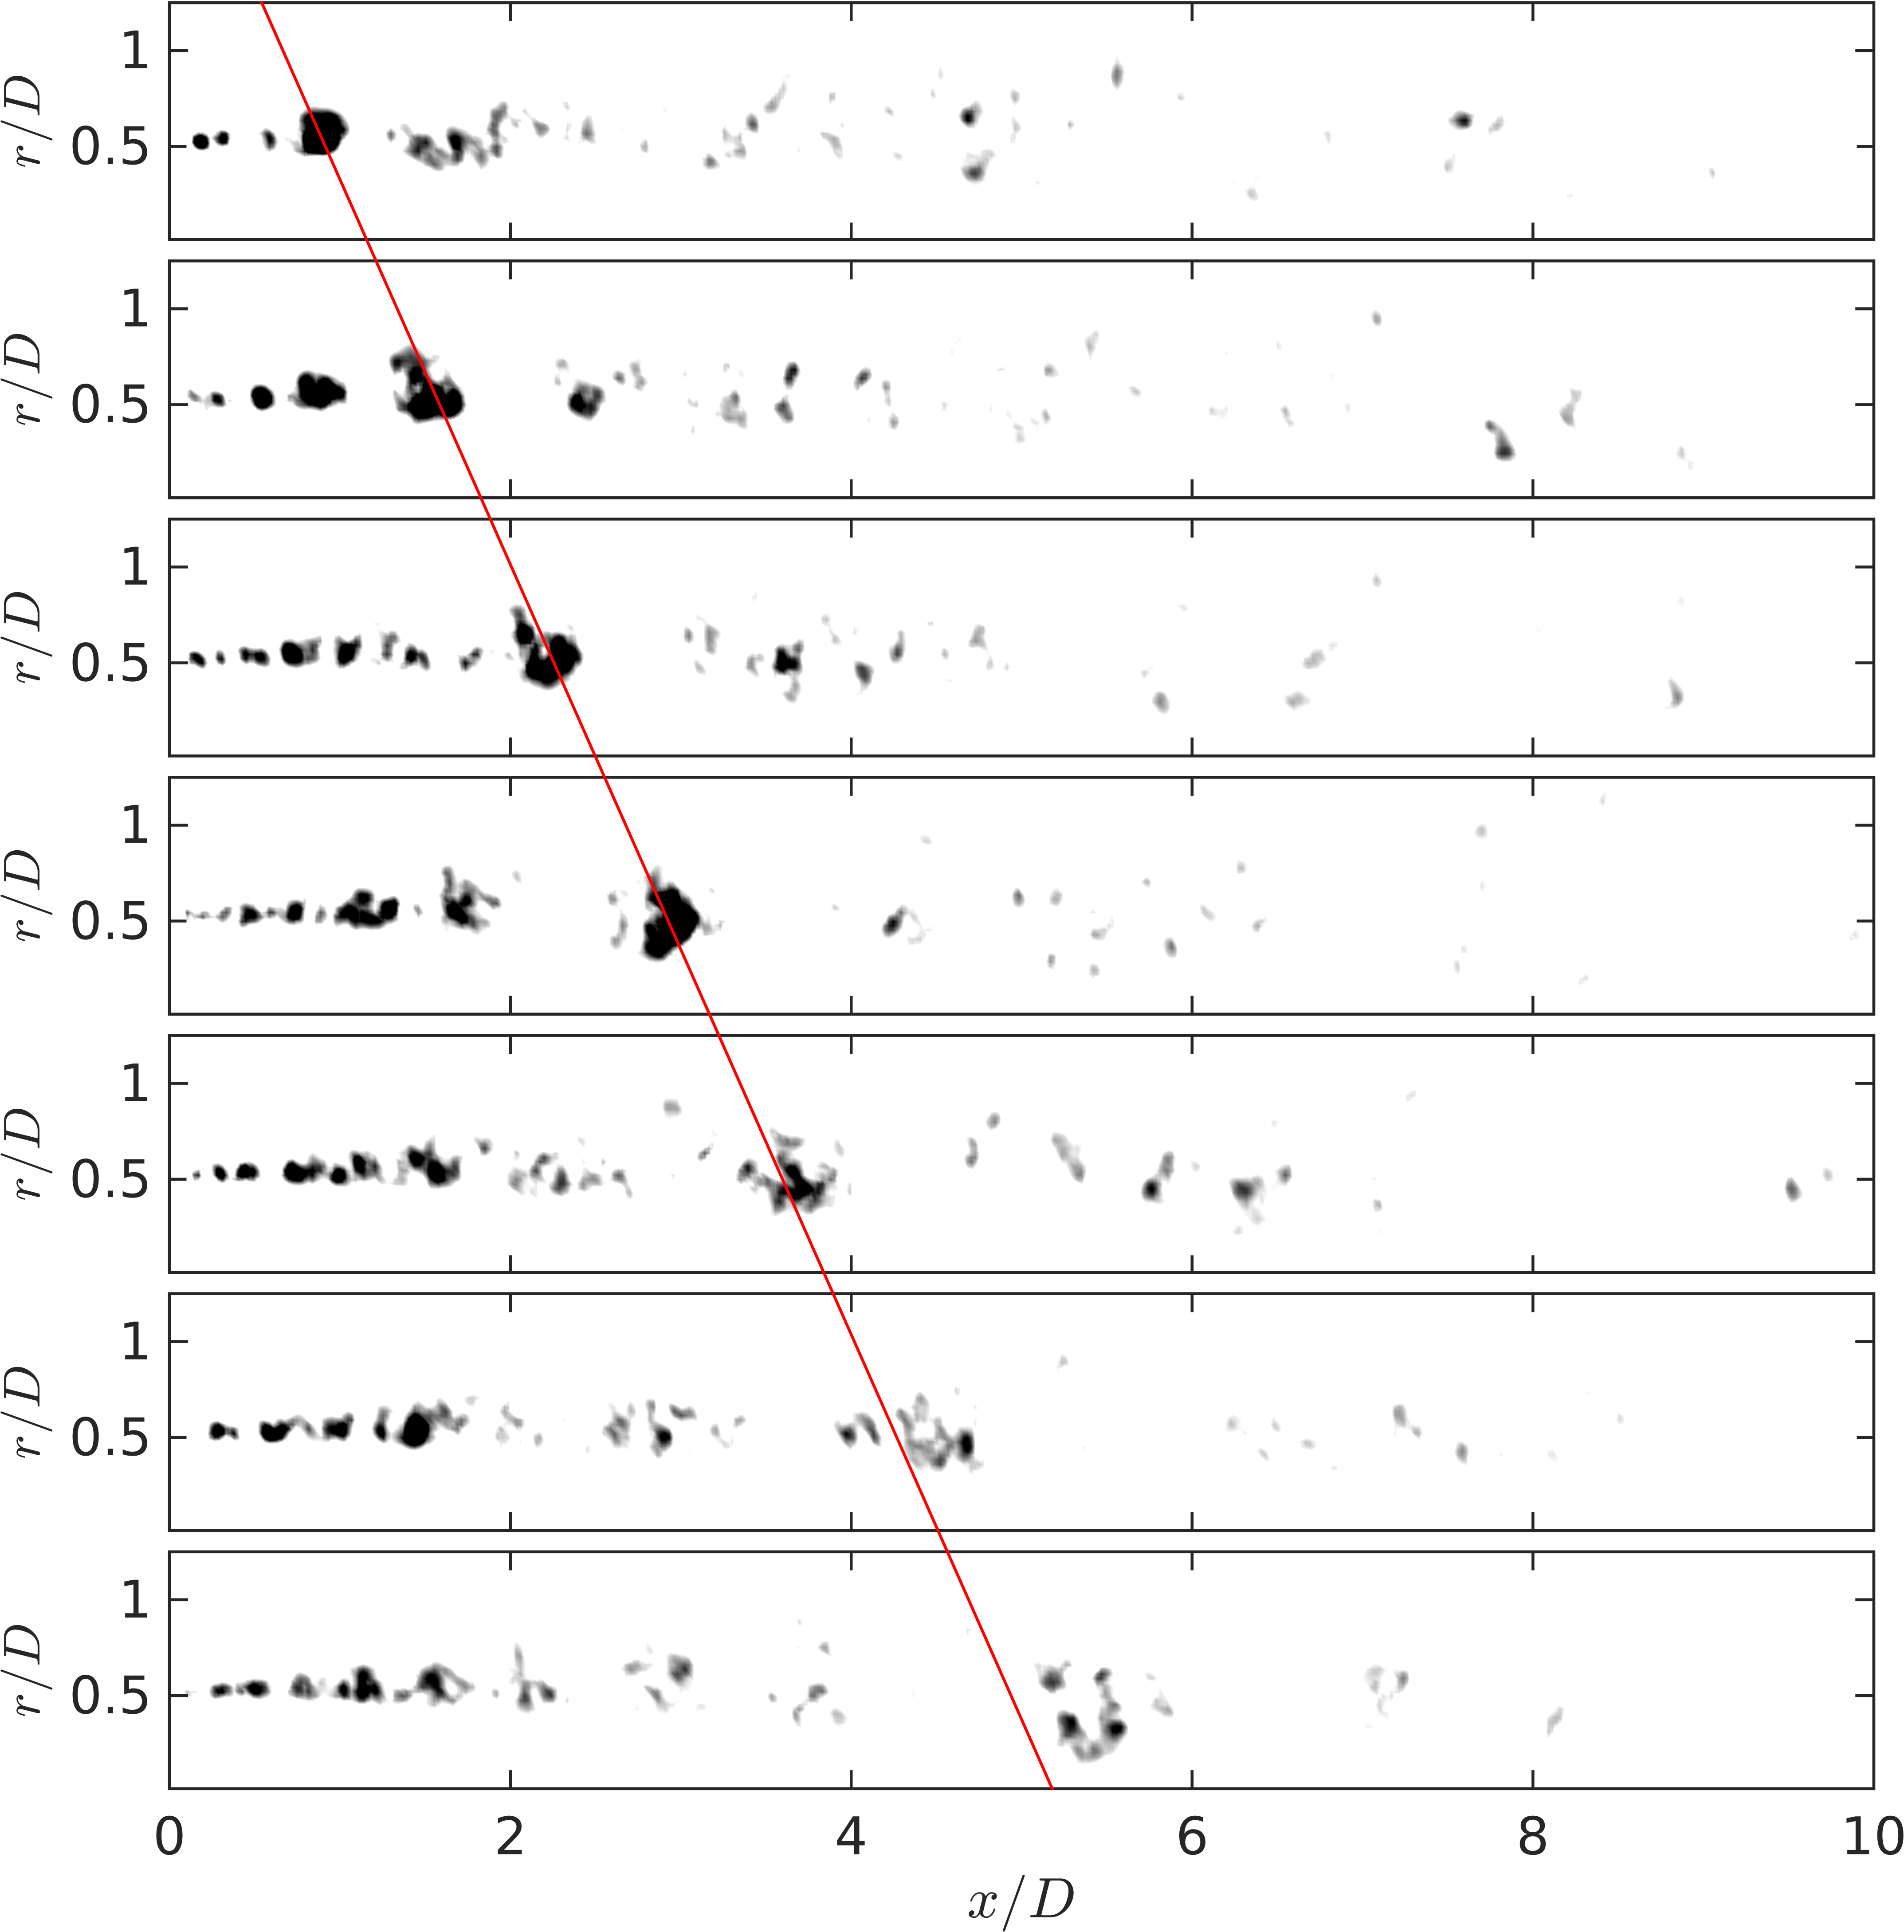
\includegraphics[width=5in]{Figures/ch4_St005_lambda.png}
	\caption{Evolution of the independent vortex ring ($St_{DF}=0.05$), as visualized using swirling strength. Images are shown at constant phase steps of roughly $\pi/8$, starting with a phase of $\pi/4$.}
	\label{fig:ch4_impulse_structure_disintegration}
\end{figure}

As already known from prior experiments at the GDTL \citep{Kearney-Fischer2009}, the excitation produces a strong roll-up of vortical (toroidal) fluid in the near-nozzle region; in the present case the large-scale structure generated by the excitation is clearly discernible over the background turbulence (and experimental/computational noise) by $x/D \simeq 1$.
The rapid growth of the vortex slows by $x/D \simeq 1.5$ and it advects downstream relatively unchanged until  $x/D \simeq 4$.
It is at this point that the vortex undergoes a rapid disintegration, yielding smaller scale, less coherent structures (though by no means would these structures be classified as fine-scale turbulence) as it passes through the end of the potential core.
These results are in general agreement with those of \citet{Hileman2005}, who found that the large-amplitude acoustic bursts of energy were associated with the passage of high-order structures through the end of the potential core.
\begin{figure}
	\centering
%	\begin{subfigure}{1\textwidth}
%		\centering
		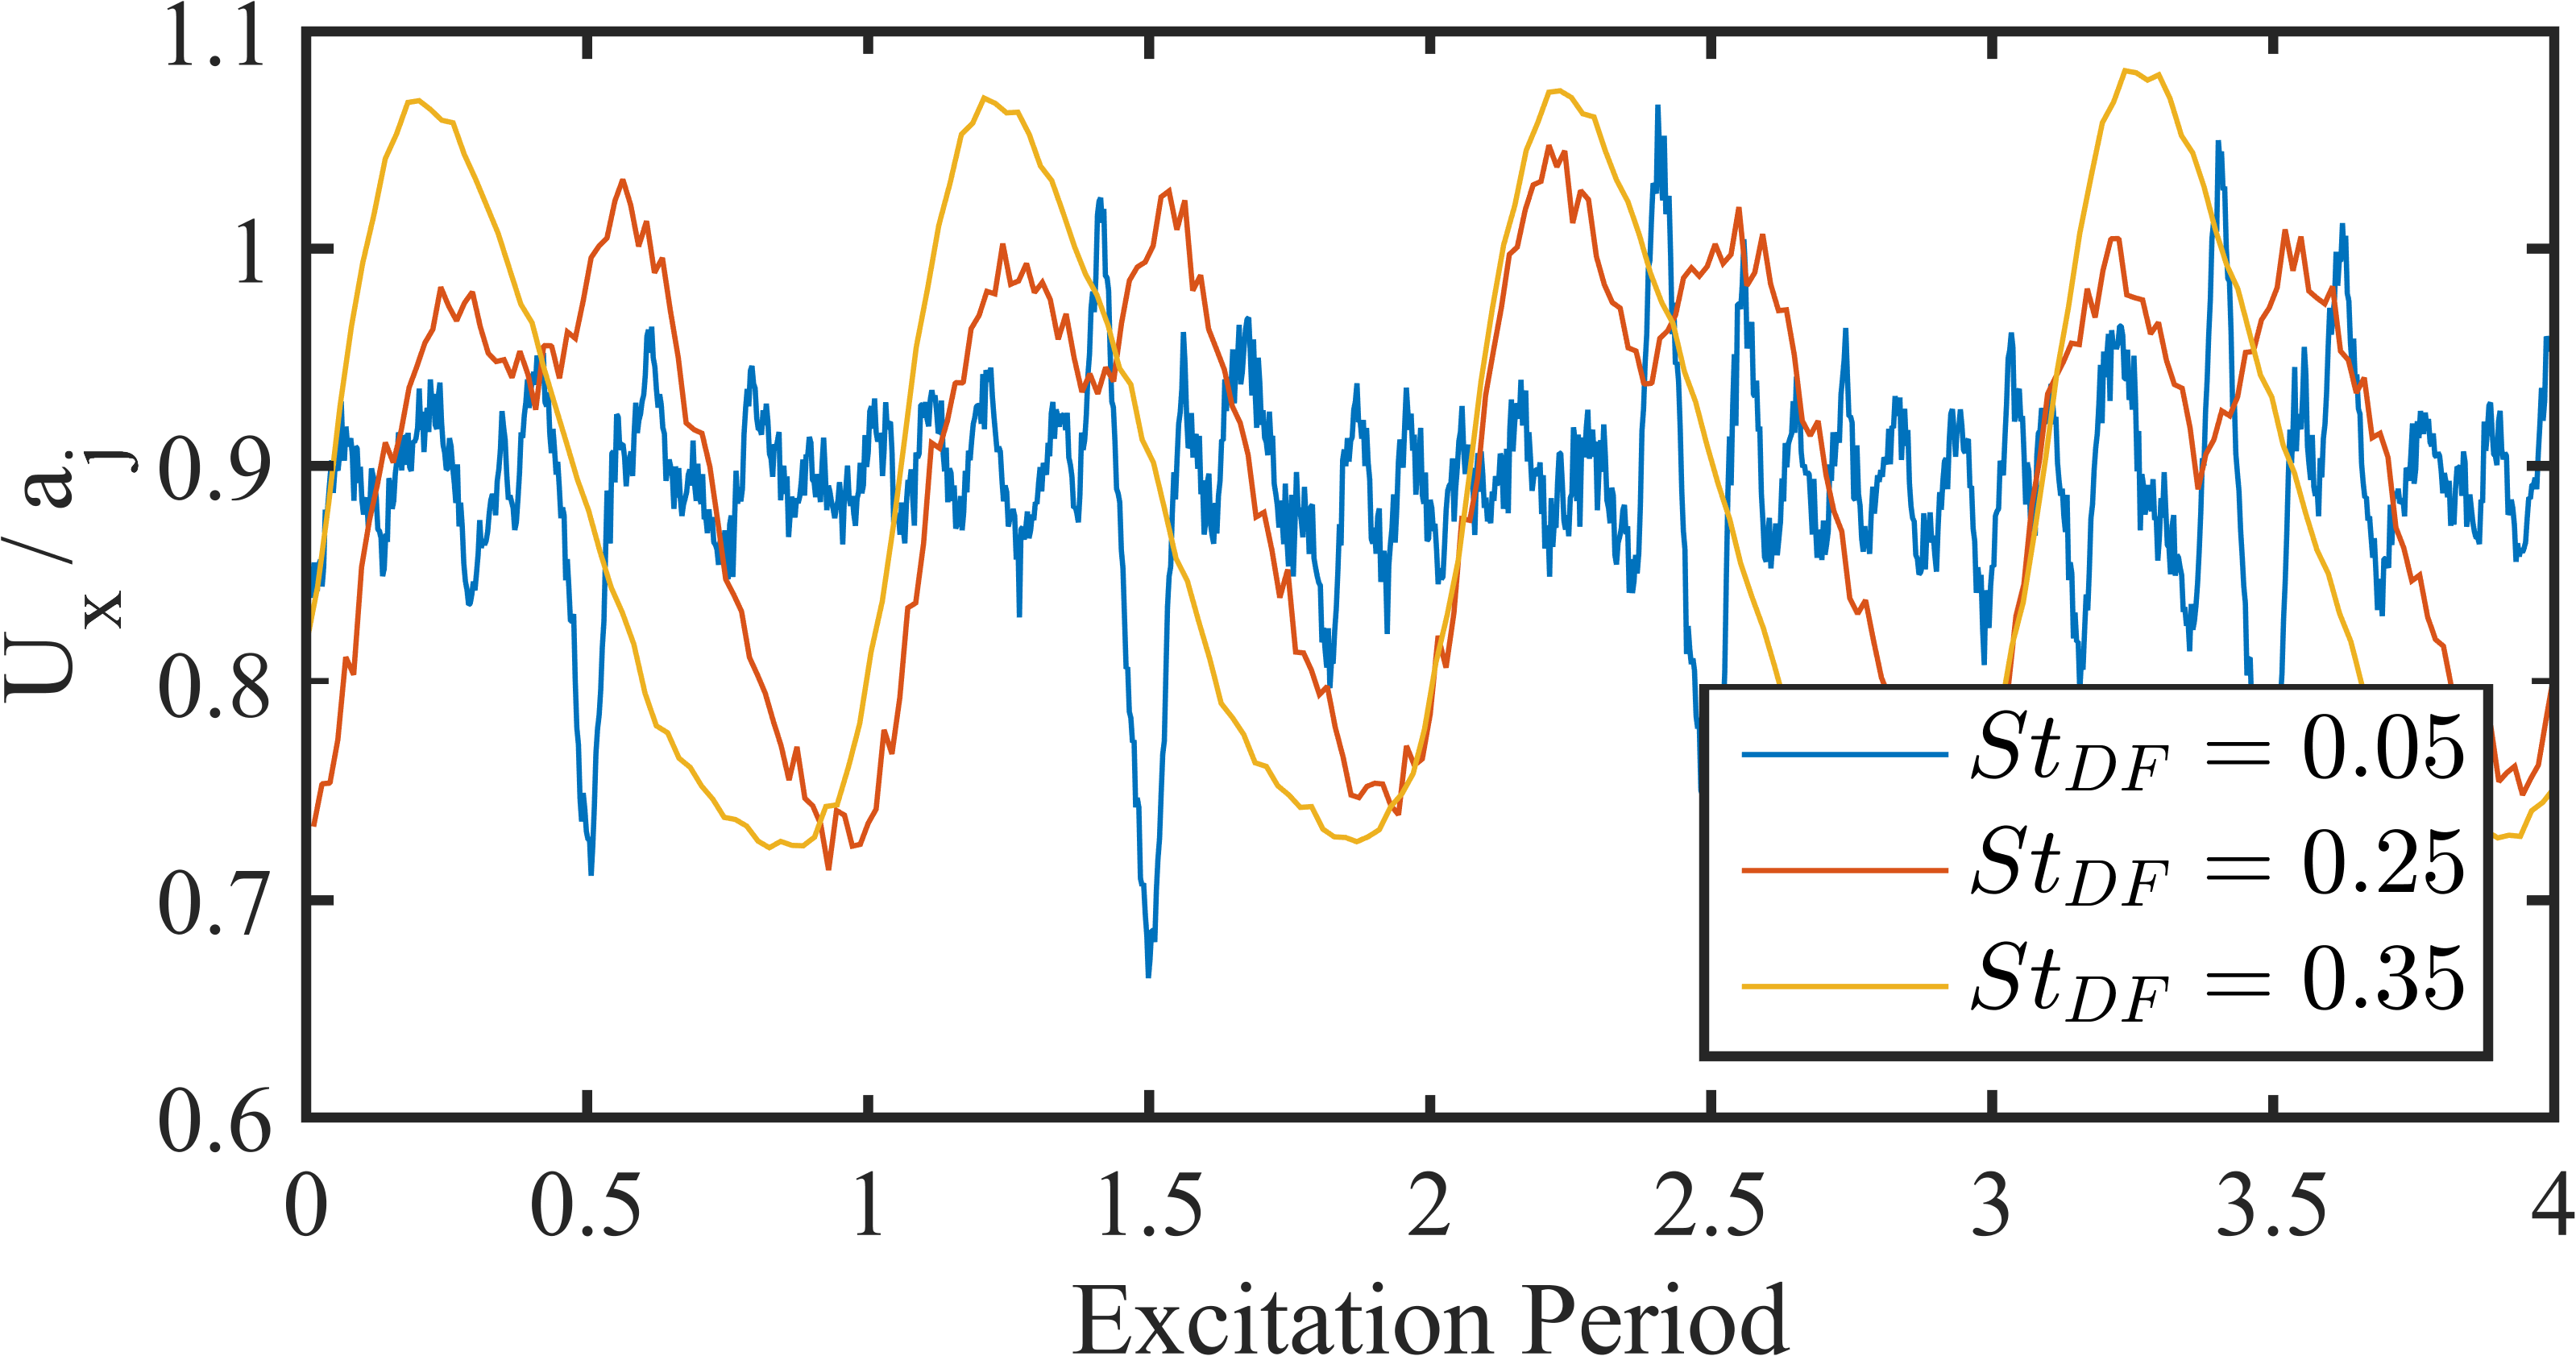
\includegraphics[width=3.5in]{Figures/ch4_centerline_mach_temporal.png} \\
%		\caption{}
%		\label{fig:ch4_centerlinemach_temporal}
%	\end{subfigure}\\
%	\begin{subfigure}{1\textwidth}
%		\centering
		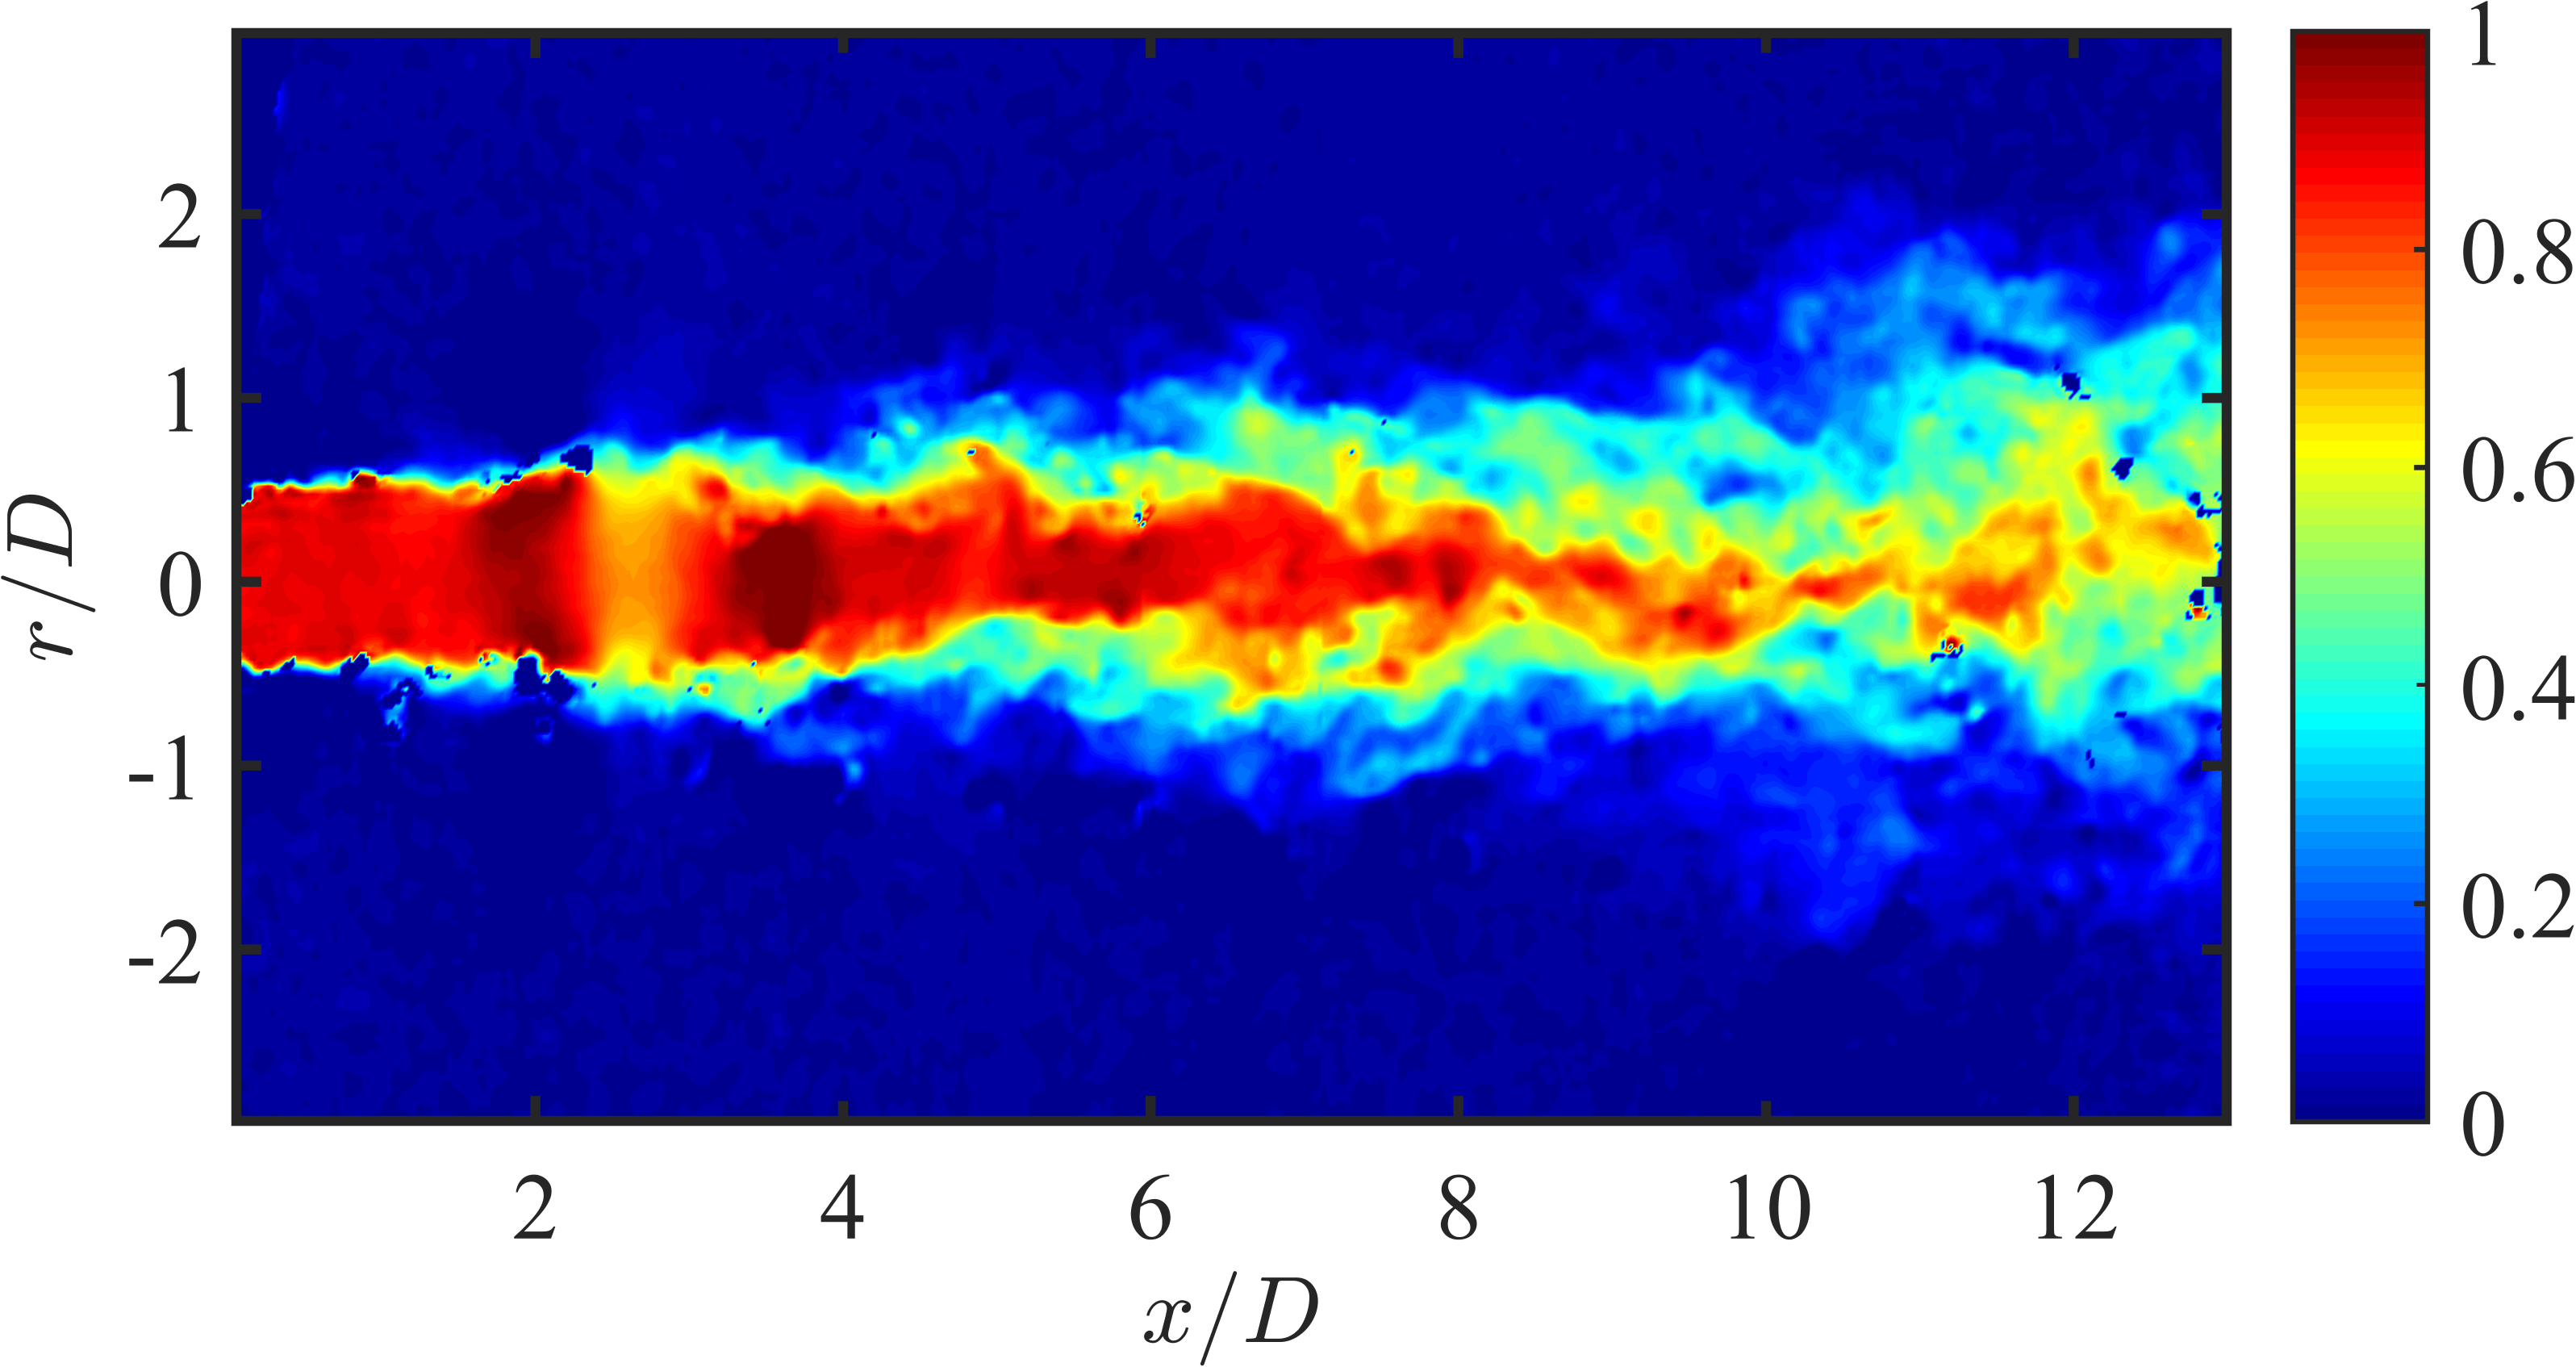
\includegraphics[width=3.5in]{Figures/ch4_rawUx_acceleration.png}
%		\caption{}
%		\label{fig:ch4_St005_rawUx_snapshot}
%	\end{subfigure}
	\caption{Fluctuations associated with the passage of large-scale structures in the axial velocity along the jet centerline at $x/D = 4$ (a) and an arbitrary raw PIV snapshot displaying similar behavior for the $St_{DF}  = 0.05$ jet(b).}
\end{figure}

Accompanying the passage of the vortical structure is a large amplitude oscillation in the axial velocity, which reaches into the potential core to the jet centerline (which is expected, given the radial profile of axisymmetric instability waves known from linear stability analysis \citep{Michalke1965}).
As shown in \fig{fig:ch4_centerlinemach_temporal}, the vortical structures are characterized by large velocity deficit, which is preceded by a large acceleration of the fluid that often crosses the sonic threshold as the vortex begins to disintegrate.
The author was surprised to see such a strong axial acceleration, however this same axial acceleration can also be found in the raw PIV snapshots that have not been post-processed by SE-POD if one looks for it (note the coherent region of supersonic velocity just upstream of $x/D = 4$ in \fig{fig:ch4_St005_rawUx_snapshot}).
An acceleration of the less-coherent structures can also be observed in \fig{fig:ch4_impulse_structure_disintegration}, as the small eddies are located further downstream in the final frames than they would be if following a constant convective velocity (as denoted by the red line overlain on the frames).
As discussed by \citet{Tam1996} (among others), the aeroacoustic efficiency of structures increases with Mach number and envelope modulation.
Therefore, the twin effects of rapid disintegration (i.e. rapid envelope modulation) and acceleration around $x/D \simeq 4$ would to greatly enhance the acoustic efficiency from the vortex.
This potentially explains why the region in which the turbulent structure rapidly disintegrates appears to dominate over the region in which the turbulent structure rapidly grows in terms of the noise emission per the results of ???.

\subsection{Coherent Structure Merging}
In the simulated subsonic shear layer of \citet{Wei2006}, optimized control for noise mitigation using generalized actuation was implemented using the adjoint perturbation method.
The methodology was able to affect a significant reduction in the emitted noise, though the exact mechanism by which this was accomplished was not immediately clear, even in this highly simplified flow (two-dimensional shear layer).
In \citet{Cavalieri2010b} the same numerical database was investigated with a specific focus on identifying intermittent events related to the noise generation process.
Here it was found that the control achieved the majority of the sound reduction by suppressing a single triple vortex interaction, thereby regularizing the flow and preventing the generation of high-amplitude peaks in the acoustic field.
The results of \citet{Kibens1980} also identified vortex merging as a prominent noise source in a (low) subsonic jet.
With this in mind, the evolution of the vortices in the periodically excited jets was analyzed.
%
\fig{fig:ch4_period_structure_disintegration} illustrates a complete excitation period for the $St_{DF} = 0.25$ excited jet; as before the velocity fields were smoothed prior to computation of the swirling strength, and the results have been phase-averaged over roughly 150 phases.
Previous analysis of the near-field had used two-point correlations between subsequent microphones in order to estimate the convective velocity of the large-scale structures; based on the time-lag for the maximum correlation value, the convective velocity was estimated as $U_c \simeq 0.7 U_j$.
However, the analysis of \citet{Speth2015} in a simulated Mach 0.9 unheated jet found that this method over-predicted the convective velocity; for example, near the end of the potential core two-point correlations in the irrotational near-field produced an estimate of $U_c \simeq 0.67 U_j$ whereas correlations in the \textit{flow}-field produced an estimate of $U_c \simeq 0.64 U_j$.
Essentially, the energy of the acoustic field in the irrotational near-field though small, is non-trivial, and as a result the much higher propagation velocity for the acoustic energy skews the convective velocity estimate to slightly higher values.
By using only the hydrodynamic component of the near-field (produced by the decomposition of ???, the convective velocity was estimated as $U_c \simeq 0.54 U_j$ near the nozzle exit and $U_c \simeq 0.65 U_j$ near the end of the potential core (which, incidentally, are nearly identical to the values reported in \citet{Speth2015}).
Based on these values, the vortex spacing is expected to be $\simeq 2.6D$ near the end of the potential core.
\begin{figure}
	\centering
	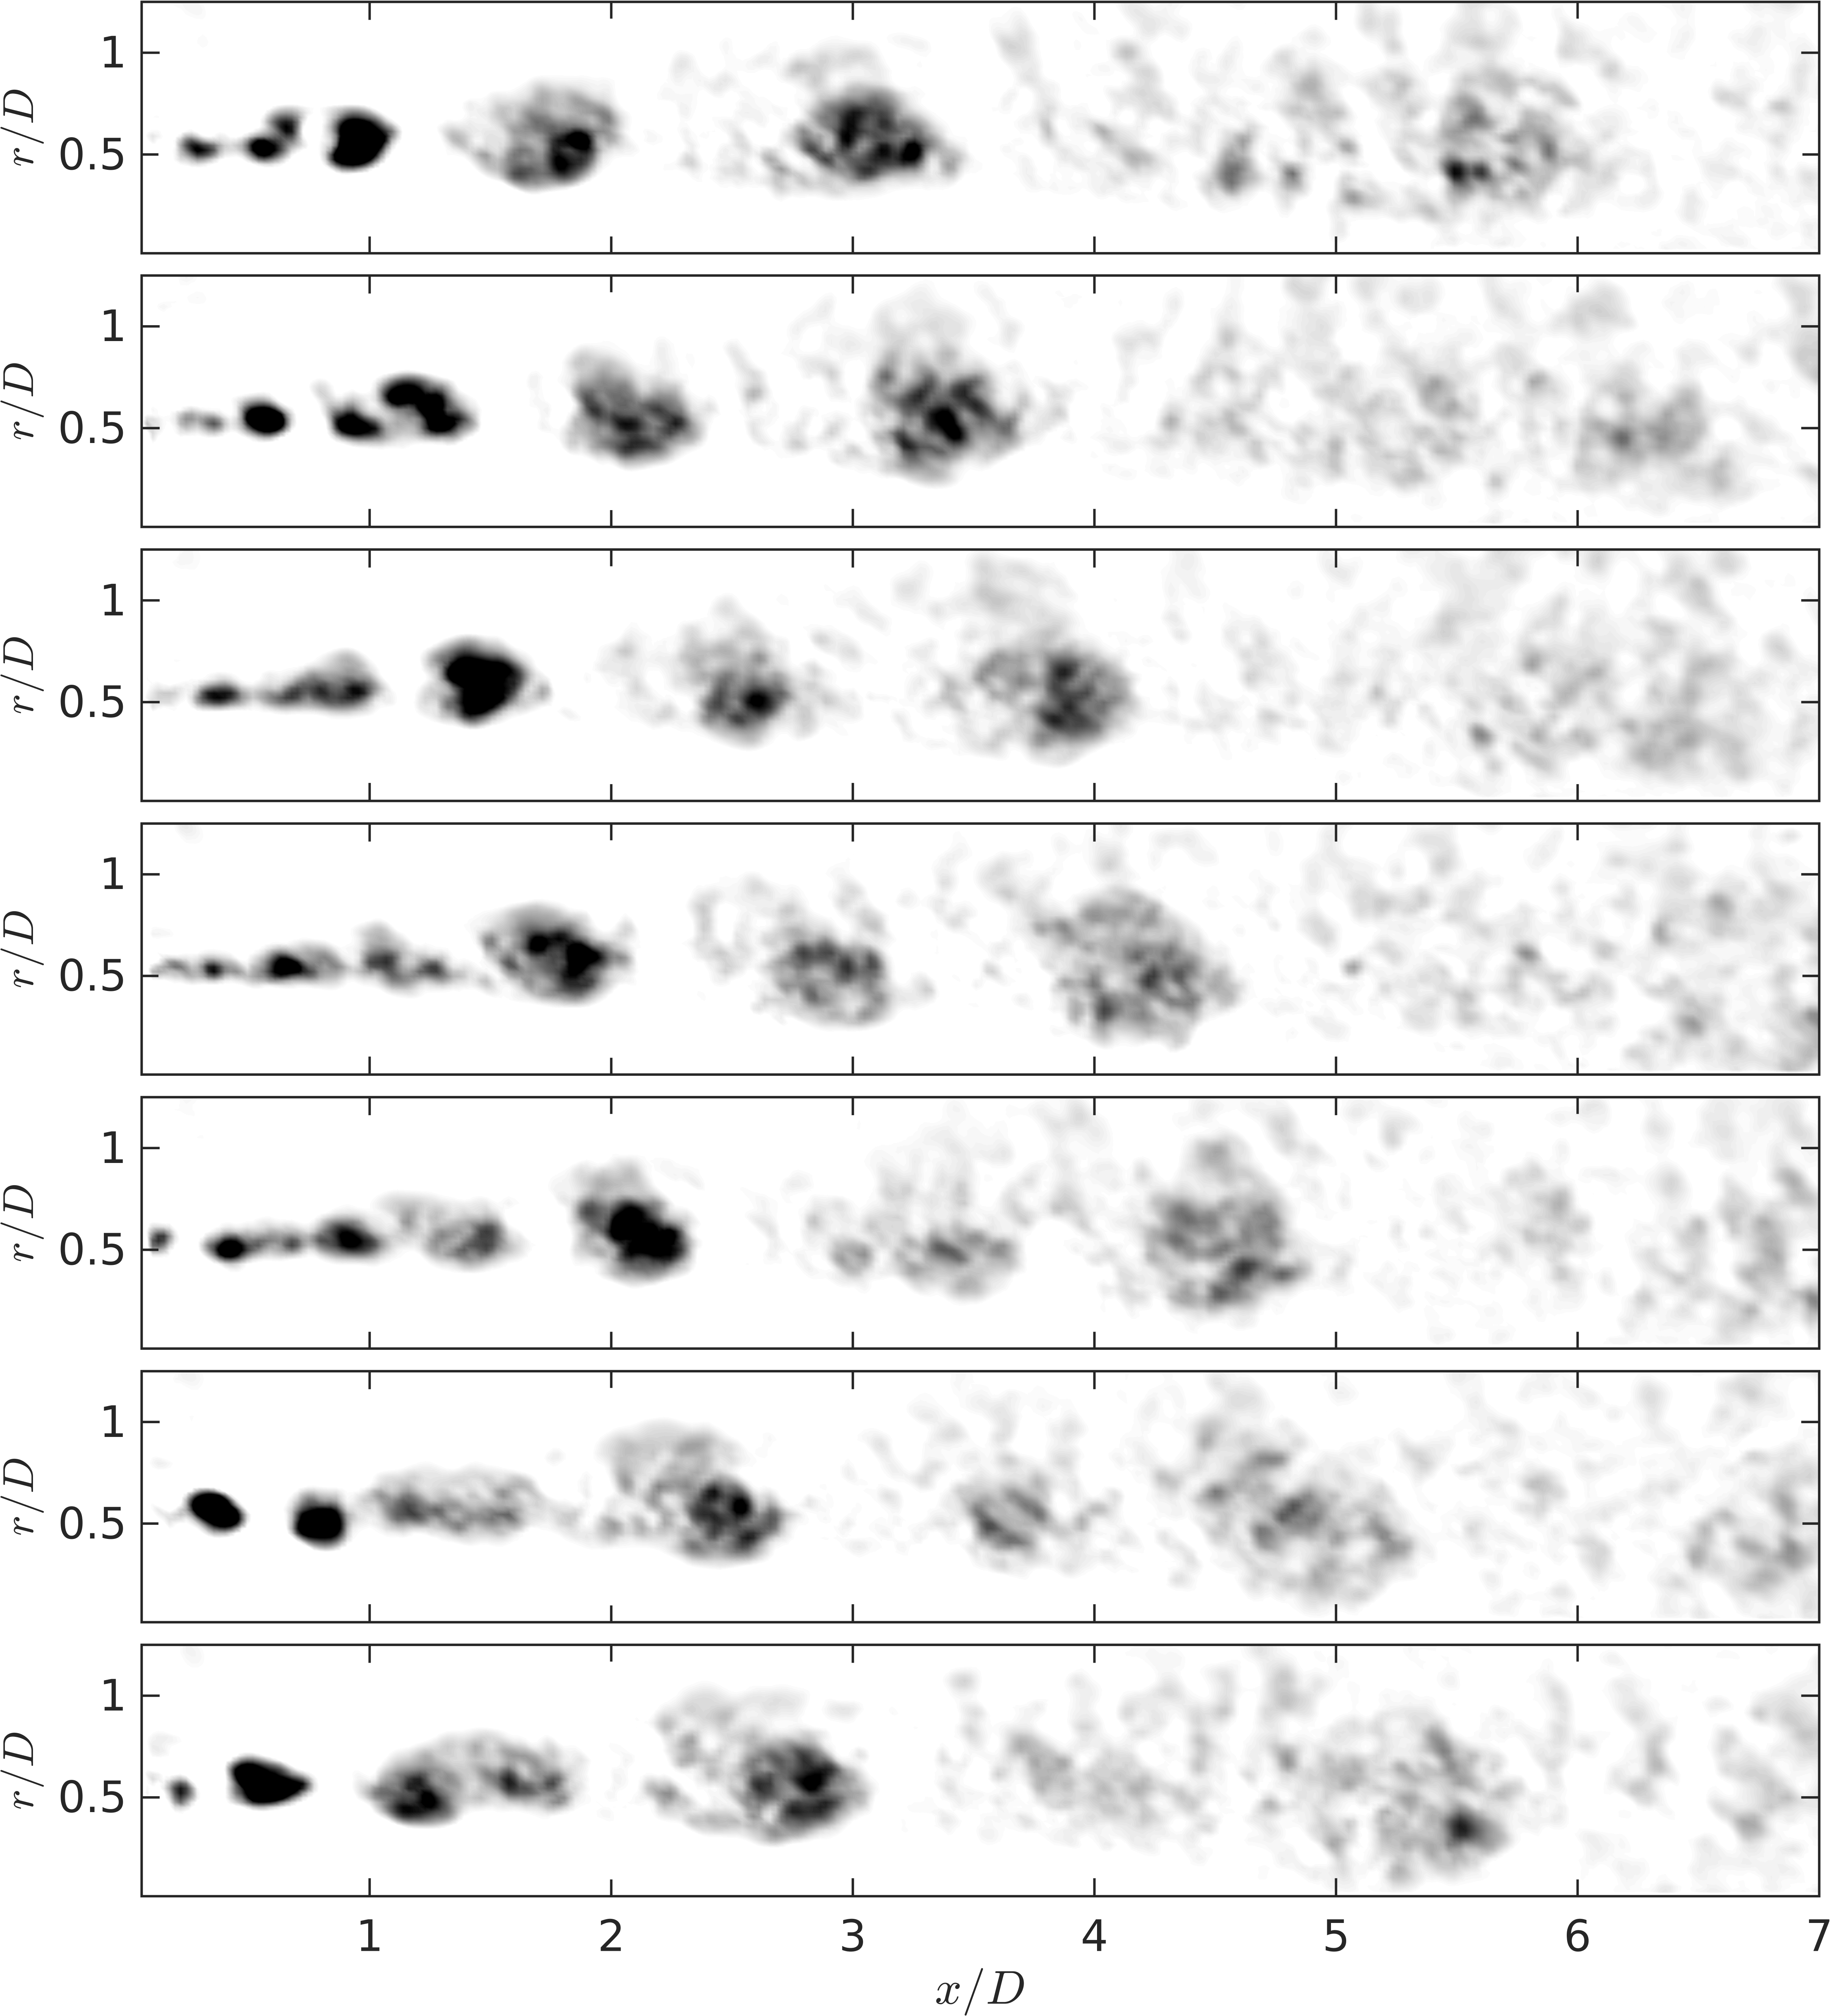
\includegraphics[width=5in]{Figures/ch4_St025_lambda.png}
	\caption{Evolution of the periodic vortex ring ($St_{DF}=0.25$), as visualized using swirling strength. One complete actuation period is shown.}
	\label{fig:ch4_period_structure_disintegration}
\end{figure}

As expected, the excitation produces a periodic roll-up of large-scale structures which, in the downstream region near the end of the potential core, roughly match with the vortex spacing for this frequency (see frame 1 in \fig{fig:ch4_period_structure_disintegration}).
However, in the upstream region ($x/D < 2$) the vortex spacing halves - the LAFPA excitation is in fact producing structures with a frequency associated with the most unstable shear layer frequency, which is significantly higher than the jet column mode frequency.
While this is the first time that this behavior has been observed at the GDTL, it is not terribly surprising if the specifics of LAFPA actuation are considered with respect to the well-known shear layer instability characteristics.
Unlike many other actuators used previously for flow control, the perturbation generated by the LAFPAs is non-sinusoidal and comprised of many higher harmonics than just the fundamental excitation frequency.
These higher harmonics couple to the flow and excite the shear layer instability, which is most unstable at frequencies much higher than the excitation frequencies used in this work.
Therefore, the structures initially formed by the excitation are going to be associated with harmonics of the excitation frequency.
Hence, it is only after merging (or successive mergings) that the passage frequency of the large-scale structures is going to match the fundamental excitation frequency.

In frame 2, the two structures at $x/D = 1$ are beginning to merge.
The trailing structure is inducted inside the preceding structure, and by $x/D \simeq 3$ the merging process is complete.
As the resultant structure convects downstream, the beginning of the breakdown of the vortex is witnessed near $x/D \simeq 4$, similar to the results of the impulsively excited vortex ring and an acceleration of the centerline velocity to slightly supersonic speeds is also observed (\fig{fig:ch4_centerlinemach_temporal}).
Here however, a secondary interaction between structures appears to be occurring, most visibly in frames 5--7. 
Depending on how exactly the coherent vortices are visualized, it appears that a second merging process is commencing here, however the vortices disintegrate before the trailing vortices can be inducted into the first. 
As the vortex at $x/D \simeq 4.5$ is breaking down, the trailing vortex breaks down as well, in fact much more abruptly than the leading vortex; the appearance of structures now matches the excitation frequency.
As the cycle is repeated (beginning again at frame 1), these two vortices (or more accurately, the less coherent, higher-order remnants of them) are no longer individually distinguishable.

Recall that the far-field response of the jet to periodic excitation at $St_{DF}=0.35$ could not be reproduced accurately using a linear superposition of the impulse response.
The vortex dynamics that this excitation frequency produces may thus serve as an insightful contrast for understanding the noise generation phenomena.
A complete excitation cycle for $St_{DF}=0.35$ has been visualized in \fig{fig:ch4_St035_structure_disintegration}.
In this case, two merging processes are now clearly evident.
The first begins just downstream of the nozzle exit, and completes by $x/D \simeq 1.5$; the second begins at $x/D \simeq 2$ and completes relatively quickly, at $x/D \simeq 3$.
It is after this second merging process that the structure spacing now matches the expected wavelength for this excitation frequency ($\lambda \simeq 1.75D$).
As with the lower frequency excitation cases just examined, the dominant vortex (which matches the excitation frequency) undergoes a disintegration beginning around $x/D \simeq 4$.
What is particularly noteworthy here though, is that the disintegration is more rapid for the $St_{DF}=0.05$ and $0.25$ cases than the $St_{DF}=0.35$ case.
In this case, the coherent structure, though severely weakened, is distinguishable over the background noise even downstream of $x/D = 6$.
As with the other excitation frequencies, the core fluid accelerates to supersonic velocities as the large-scale structures pass through the end of the potential core.
\begin{figure}
	\centering
	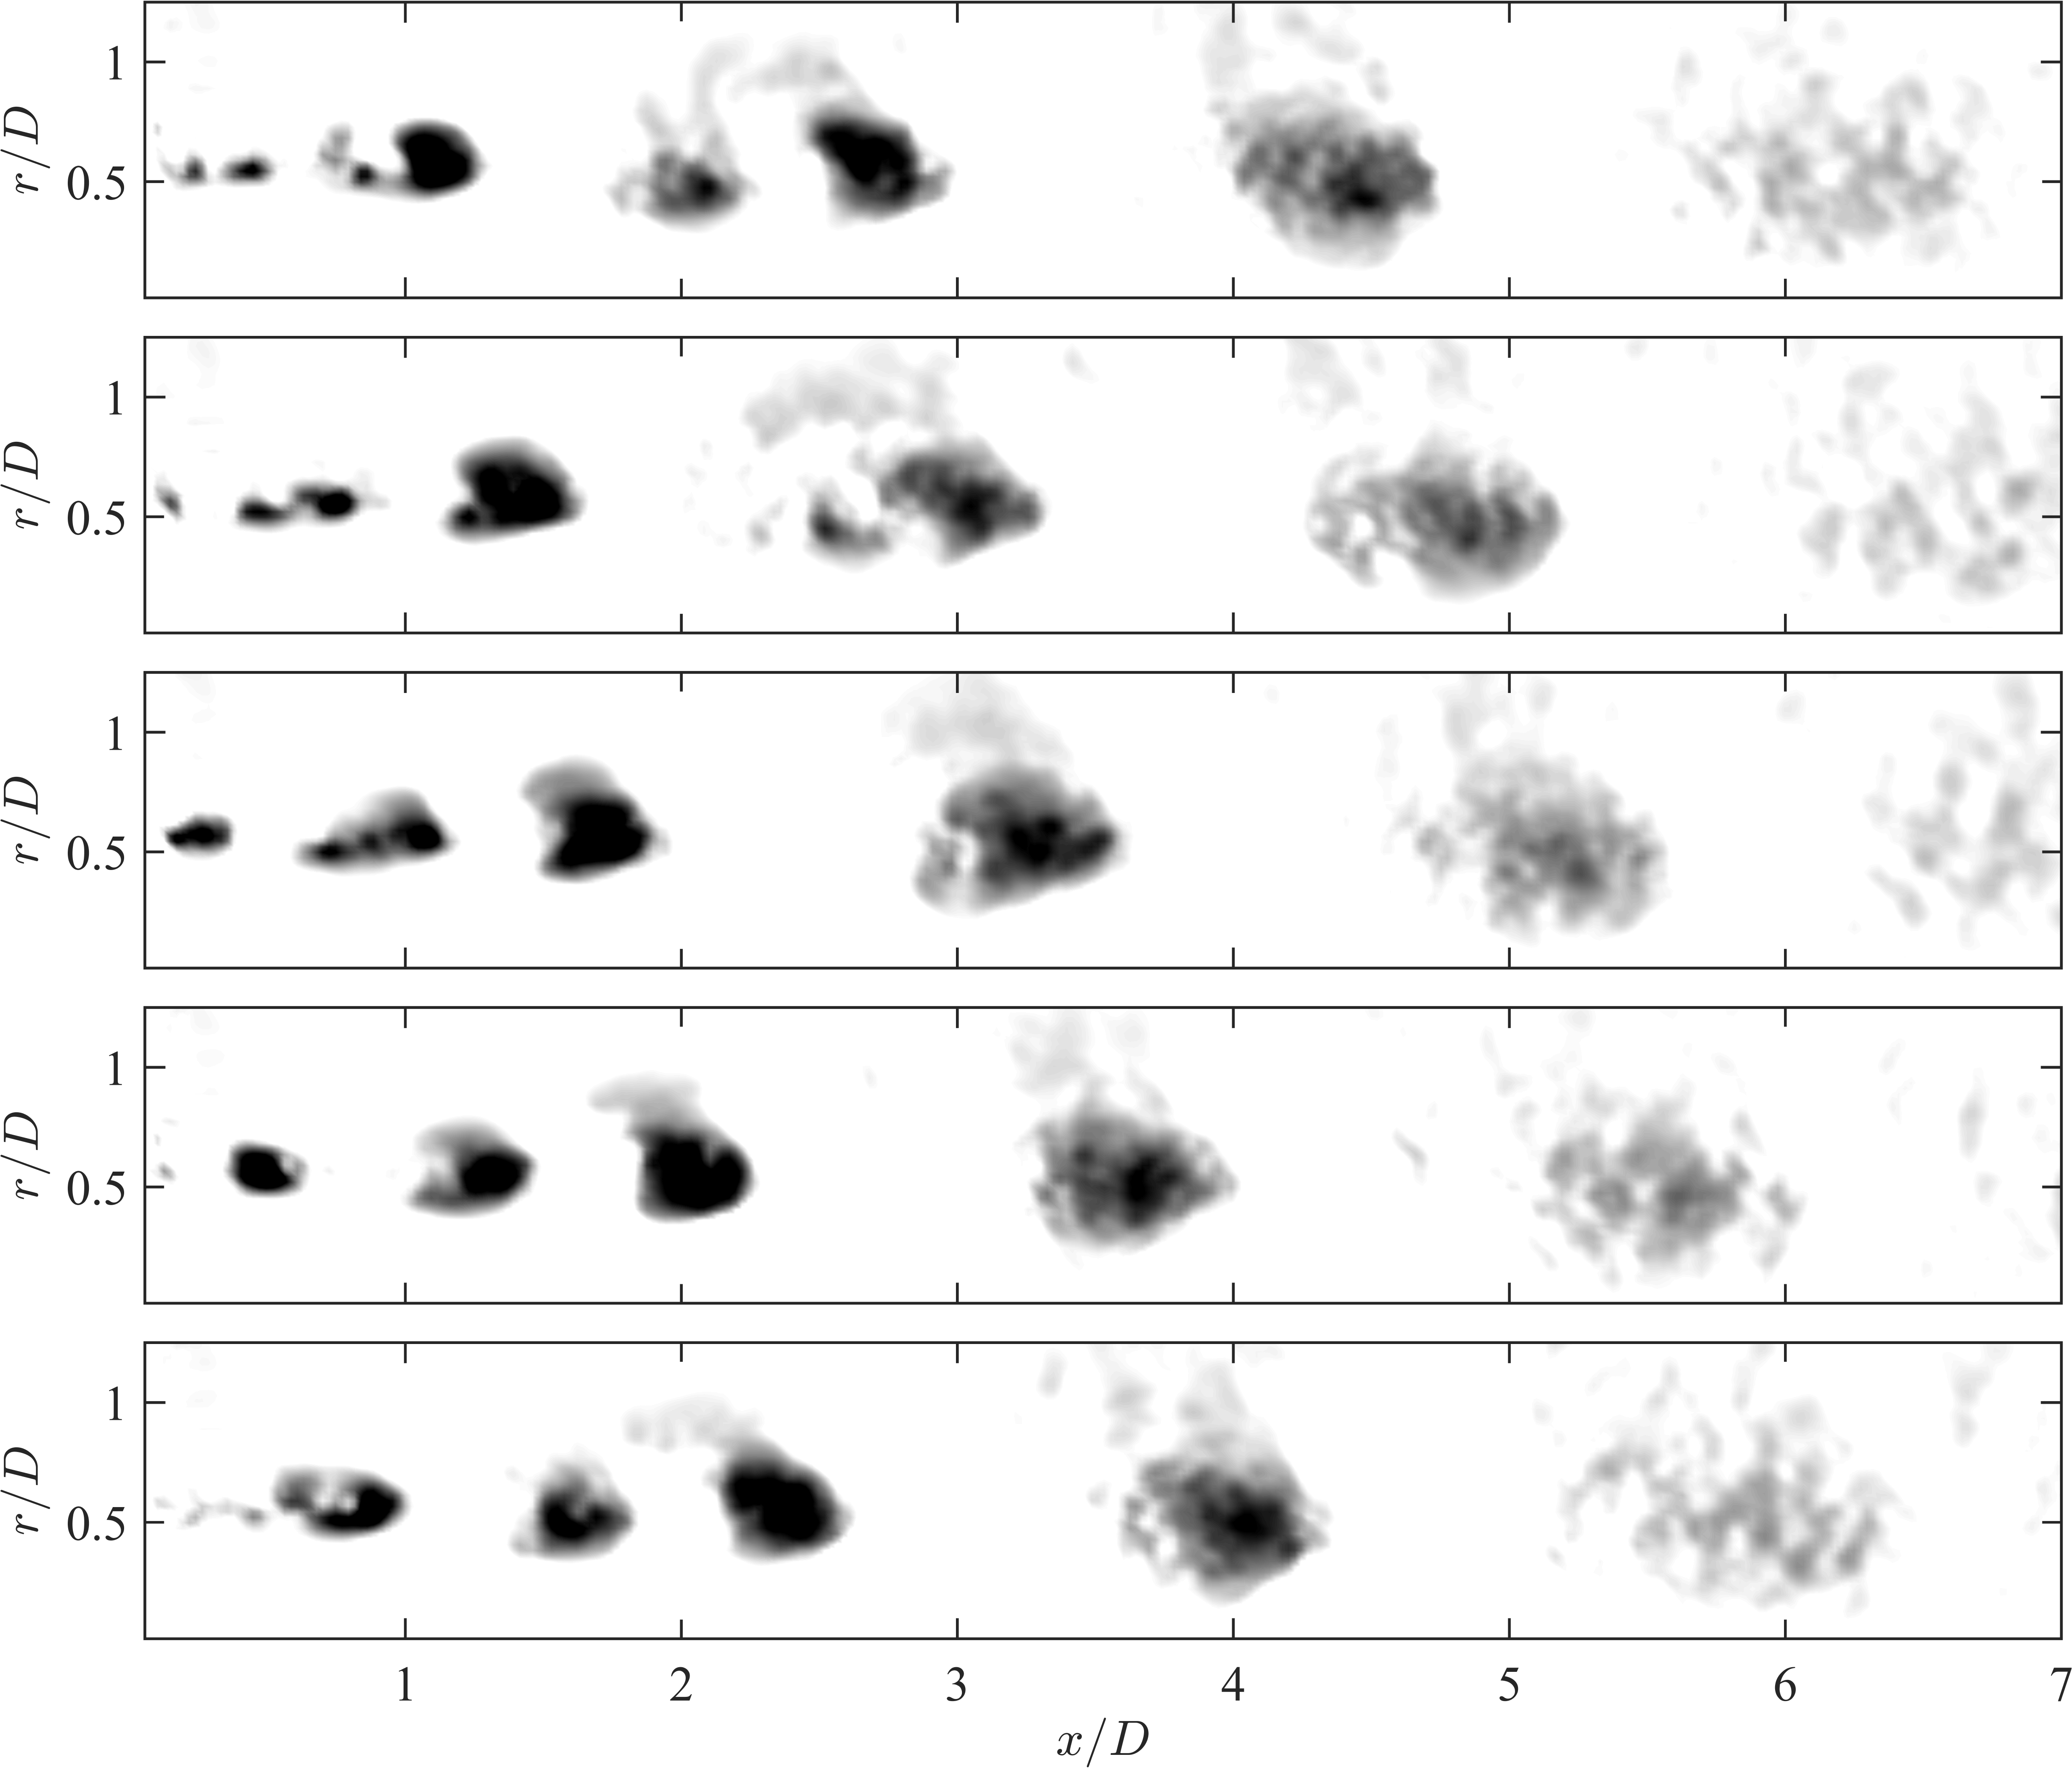
\includegraphics[width=5in]{Figures/ch4_St035_lambda_evolution.png}
	\caption{Evolution of the periodic vortex ring ($St_{DF}=0.35$), as visualized using swirling strength. One complete actuation period is shown.}
	\label{fig:ch4_St035_structure_disintegration}
\end{figure}

Clearly (and unsurprisingly), the vortex interactions in the periodically-excited jets are far more complex than the impulsively excited jet.
However, as was seen both in terms of the far-field response (\fig{fig:ch3_farfield}) as well as the acoustic source region estimated from the decomposed near-field (\fig{fig:ch3_xcorrOA}), the acoustic fields for $St_{DF}=0.05$ and $St_{DF}=0.25$ show remarkable similarity, at least at angles close to the jet axis.
Therefore, this implies that for this excitation range, the added complexity of the periodic excitation (harmonic structures, vortex merging) are not the primary drivers for noise emission (though they may still play a role).
The consistent, rapid breakdown of the LAFPA-induced structures near $x/D \simeq 4$ and accompanying fluid acceleration in both excited jets appears to be the dominant noise source. 
In contrast, the far-field acoustic response to excitation at $St_{DF}=0.35$ is not accurately reproduced by a linear superposition of the impulse response of the jet.
Analysis of the vortex dynamics demonstrates multiple merging processes occurring for this excitation frequency, and though the dominant vortex breaks down at $x/D \simeq 4$, this process is far less dramatic than in the lower-frequency excitation cases.
In this case, the merging process may in fact be a significant factor in the noise generation process.
In order to more conclusively link this behavior to the noise emission directly, in \sect{sect:source} the aeroacoustic source term will be calculated from the estimated time-resolved velocity fields using a simplified form of Lighthill's acoustic analogy.
\section{The Aeroacoustic Source Field}
\label{sect:source}
Ribner presented an alternative approach to Lighthill's acoustic analogy which posited fluctuating fluid dilatations as the source of aeroacoustic emission \citep{Ribner1962}.
This is a reinterpretation of Lighthill's source, which in subsonic, unheated, turbulent jets consists of fluctuating momentum flux.
The driving factor behind Ribner's analysis is the conceptual simplification of the aeroacoustic sources: Lighthill's quadrupoles are replaced by the contraction or expansion of fluid elements (confusingly identified alternatively as \emph{pseudosound} or \emph{pseudo-pressure}) due to the fluctuating momentum flux, which in turn drive the acoustic field.
This conceptual simplicity makes the dilatation-based approach to the acoustic analogy particularly attractive to the experimentalist for high-speed (though subsonic), turbulent flows.
The analysis, described briefly in the subsequent section, is (relatively) simple to perform computationally, relying exclusively on second-order derivatives (unlike the third-order differential equation derived by \citet{Lilley2003}) which include a natural filtering mechanism.
More importantly, the pseudosound field (which is the direct precursor to the source field) can be directly compared against the time-resolved hydrodynamic pressure field measured in the irrotational near-field, thus serving as a helpful validation of the computations.

Ribner's analysis follows directly from Lighthill's; the source term is first reduced by neglecting viscosity and entropic fluctuations (thereby assuming that the flow is of high Reynolds number and unheated), leaving only the Reynolds stress terms:
\begin{equation}
	\frac{1}{c^2}\frac{\partial^2 p}{\partial t^2} - \nabla^2 p = \nabla \cdot \nabla \cdot \rho \mathbf{u} \otimes \mathbf{u}.
\end{equation}
Ribner then split the pressure fluctuations into an acoustic component and an incompressible component (pseudosound, which is associated with the convective hydrodynamic fluctuations), $p' + p_0 = p_a + p_s$. 
The incompressible component of the flow will then satisfy
\begin{equation}
	 \rho \frac{\partial}{\partial t} (\nabla \cdot \mathbf{v} )  = 0
\end{equation}
where $\mathbf{v}$ is now used in place of $\mathbf{u}$ to signify an incompressible (solenoidal) velocity field. 
Therefore, 
\begin{equation}
	- \nabla^2 p_s = \nabla \cdot \nabla \cdot \rho_0 \mathbf{v} \otimes \mathbf{v}.
	\label{eq:solenoidal_pressure}
\end{equation}
Ribner's analysis then assumes that the full density and velocity fields can be approximated as the incompressible (solenoidal) fields (the higher-order terms scaling with the fluctuating Mach number, thus producing Ribner's dilatation equation:
\begin{equation}
	\frac{1}{c^2}\frac{\partial^2 p_a}{\partial t^2} - \nabla^2 p_a = -\frac{1}{c^2}\frac{\partial^2 p_s}{\partial t^2}.
	\label{eq:ribner_source}
\end{equation} 
In this way, acoustic pressure field is ultimately linked to the time rate of change of the dilatation (see \citet{Ristorcelli1997} for a very enlightening perturbation analysis which makes this relationship far more clear).
Numerous researchers have used the dilatation field to examine the aeroacoustic phenomena (primarily using DNS or LES simulations); see \citet{Mitchell1995}, \citet{Colonius1997}, or \citet{Freund2000} for examples.

\subsection{Numerical Methodology}
Computing the aeroacoustic source per Ribner's dilatation method from the estimated, time-resolved velocity field constitutes a three-step process. 
First, the solenoidal velocity field is computed via the Helmholtz' decomposition; the double divergence of the resulting stress tensor is then used as the source of Poisson's equation to calculate the pseudo-pressure field. 
Finally, the pseudo-pressure field is filtered in time using an energy threshold in the wavelet domain, and the second time derivative of the resultant field is computed, producing the source field.
This process is outlined in the following sections.
\subsubsection{Helmholtz Decomposition}
For a given vector field, $\mathbf{F}$, Helmholtz's theorem states that any sufficiently smooth vector field can be linearly decomposed into irrotational and solenoidal vector fields, as
\begin{equation}
\mathbf{F} = \mathbf{F}_{potential} + \mathbf{F}_{rotational} = \nabla \Phi + \nabla \times \Psi
\end{equation}
where $\Phi$ is a scalar field and $\Psi$ is a vector field.
From basic vector calculus properties, one can therefore compute these solenoidal and irrotational components by taking the divergence of this equation, leading to:
\begin{equation}
\nabla \cdot \mathbf{F} = \nabla^{2} \Phi
\end{equation}
which is simply Poisson's equation, where in the context of a velocity decomposition the forcing term is simply the divergence of the flow field (that is, the dilatation).

As only planar, not volumetric, PIV measurements were available, the azimuthal velocity and derivative terms are unknown and thus must be neglected from this analysis.
As mentioned previously, the flow-field in a natural, high Reynolds number jet is a combination of numerous azimuthal Fourier modes.
Though the velocity field has been found to contain a significant amount of energy at the higher order modes, the axisymmetric mode is still the dominant mode within the potential core region of the jet \citep{Glauser1987}.
Additionally, it is the acoustic emission from the coherent large-scale toroidal structure generated by excitation that is the primary focus of this endeavor, not the full acoustic emission from the relatively incoherent natural turbulence.
Due to the specific nature of the excitation (axisymmetric excitation), the azimuthal components of the flow are not expected to be significant.

The database of \citet{Speth2014} was provided to the authors for the purpose of validating this assumption.
Comparisons between the near-field pressure response to excitation of the experimental and numerical databases were performed in the reference, and a good match was found.
Sample results for the pressure and radial velocity field for a single azimuthal plane are shown in \fig{fig:LES_streamwise_phavg}; these results correspond to an actuation phase of $1.4 \pi$ for $St_{DF} = 0.05$, and have been phase-averaged over nine actuation cycles.
(While less than desirable, the computationalists could not store the full, instantaneous 3-D velocity fields due to harddrive limitations. The $St_{DF} = 0.05$ was therefore chosen for this analysis since it contained the fewest number of actuation cycles and thus has the highest level of incoherent fluctuations.)
From these plots, a large-scale coherent structure generated by the excitation can easily be identified, centered at $x/D = 2.1, r/D = 0.5$.
\begin{figure}
	\centering
%	\begin{subfigure}{0.75\textwidth}
%		\centering
		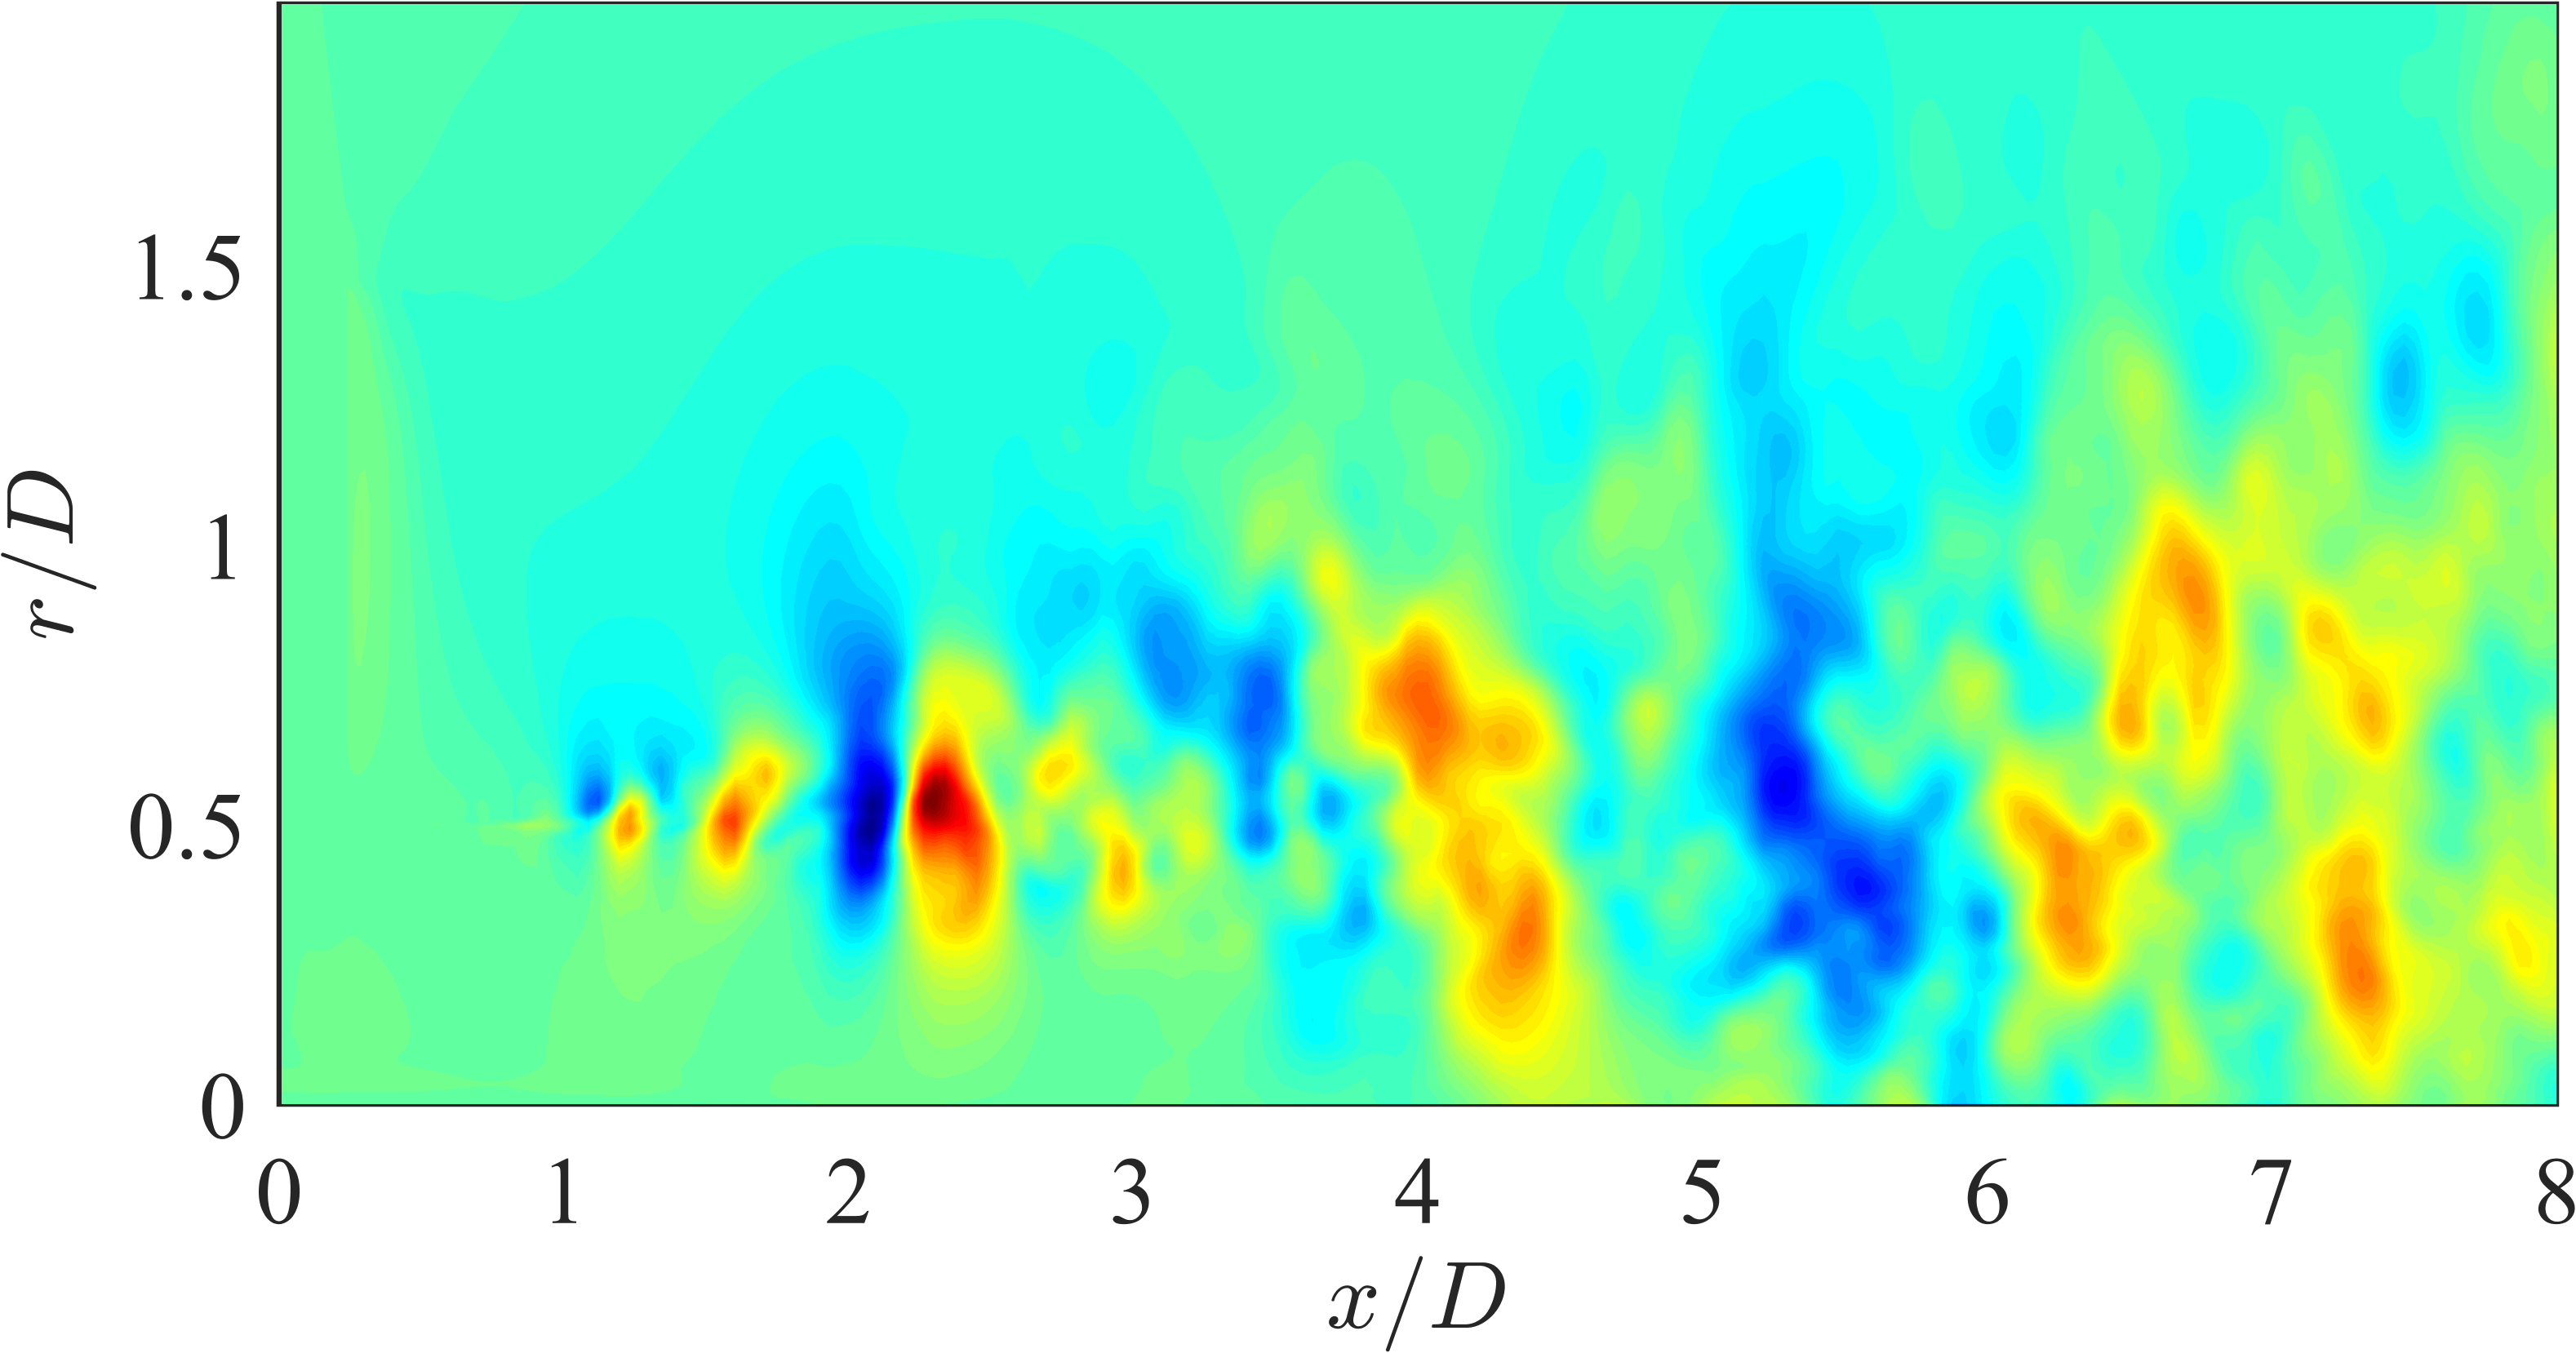
\includegraphics[width=0.6\linewidth]{Figures/LES_phavg_streamwise_Ur.png}
%		\caption{}
%	\end{subfigure}\\
%	\begin{subfigure}{0.75\textwidth}
%		\centering
		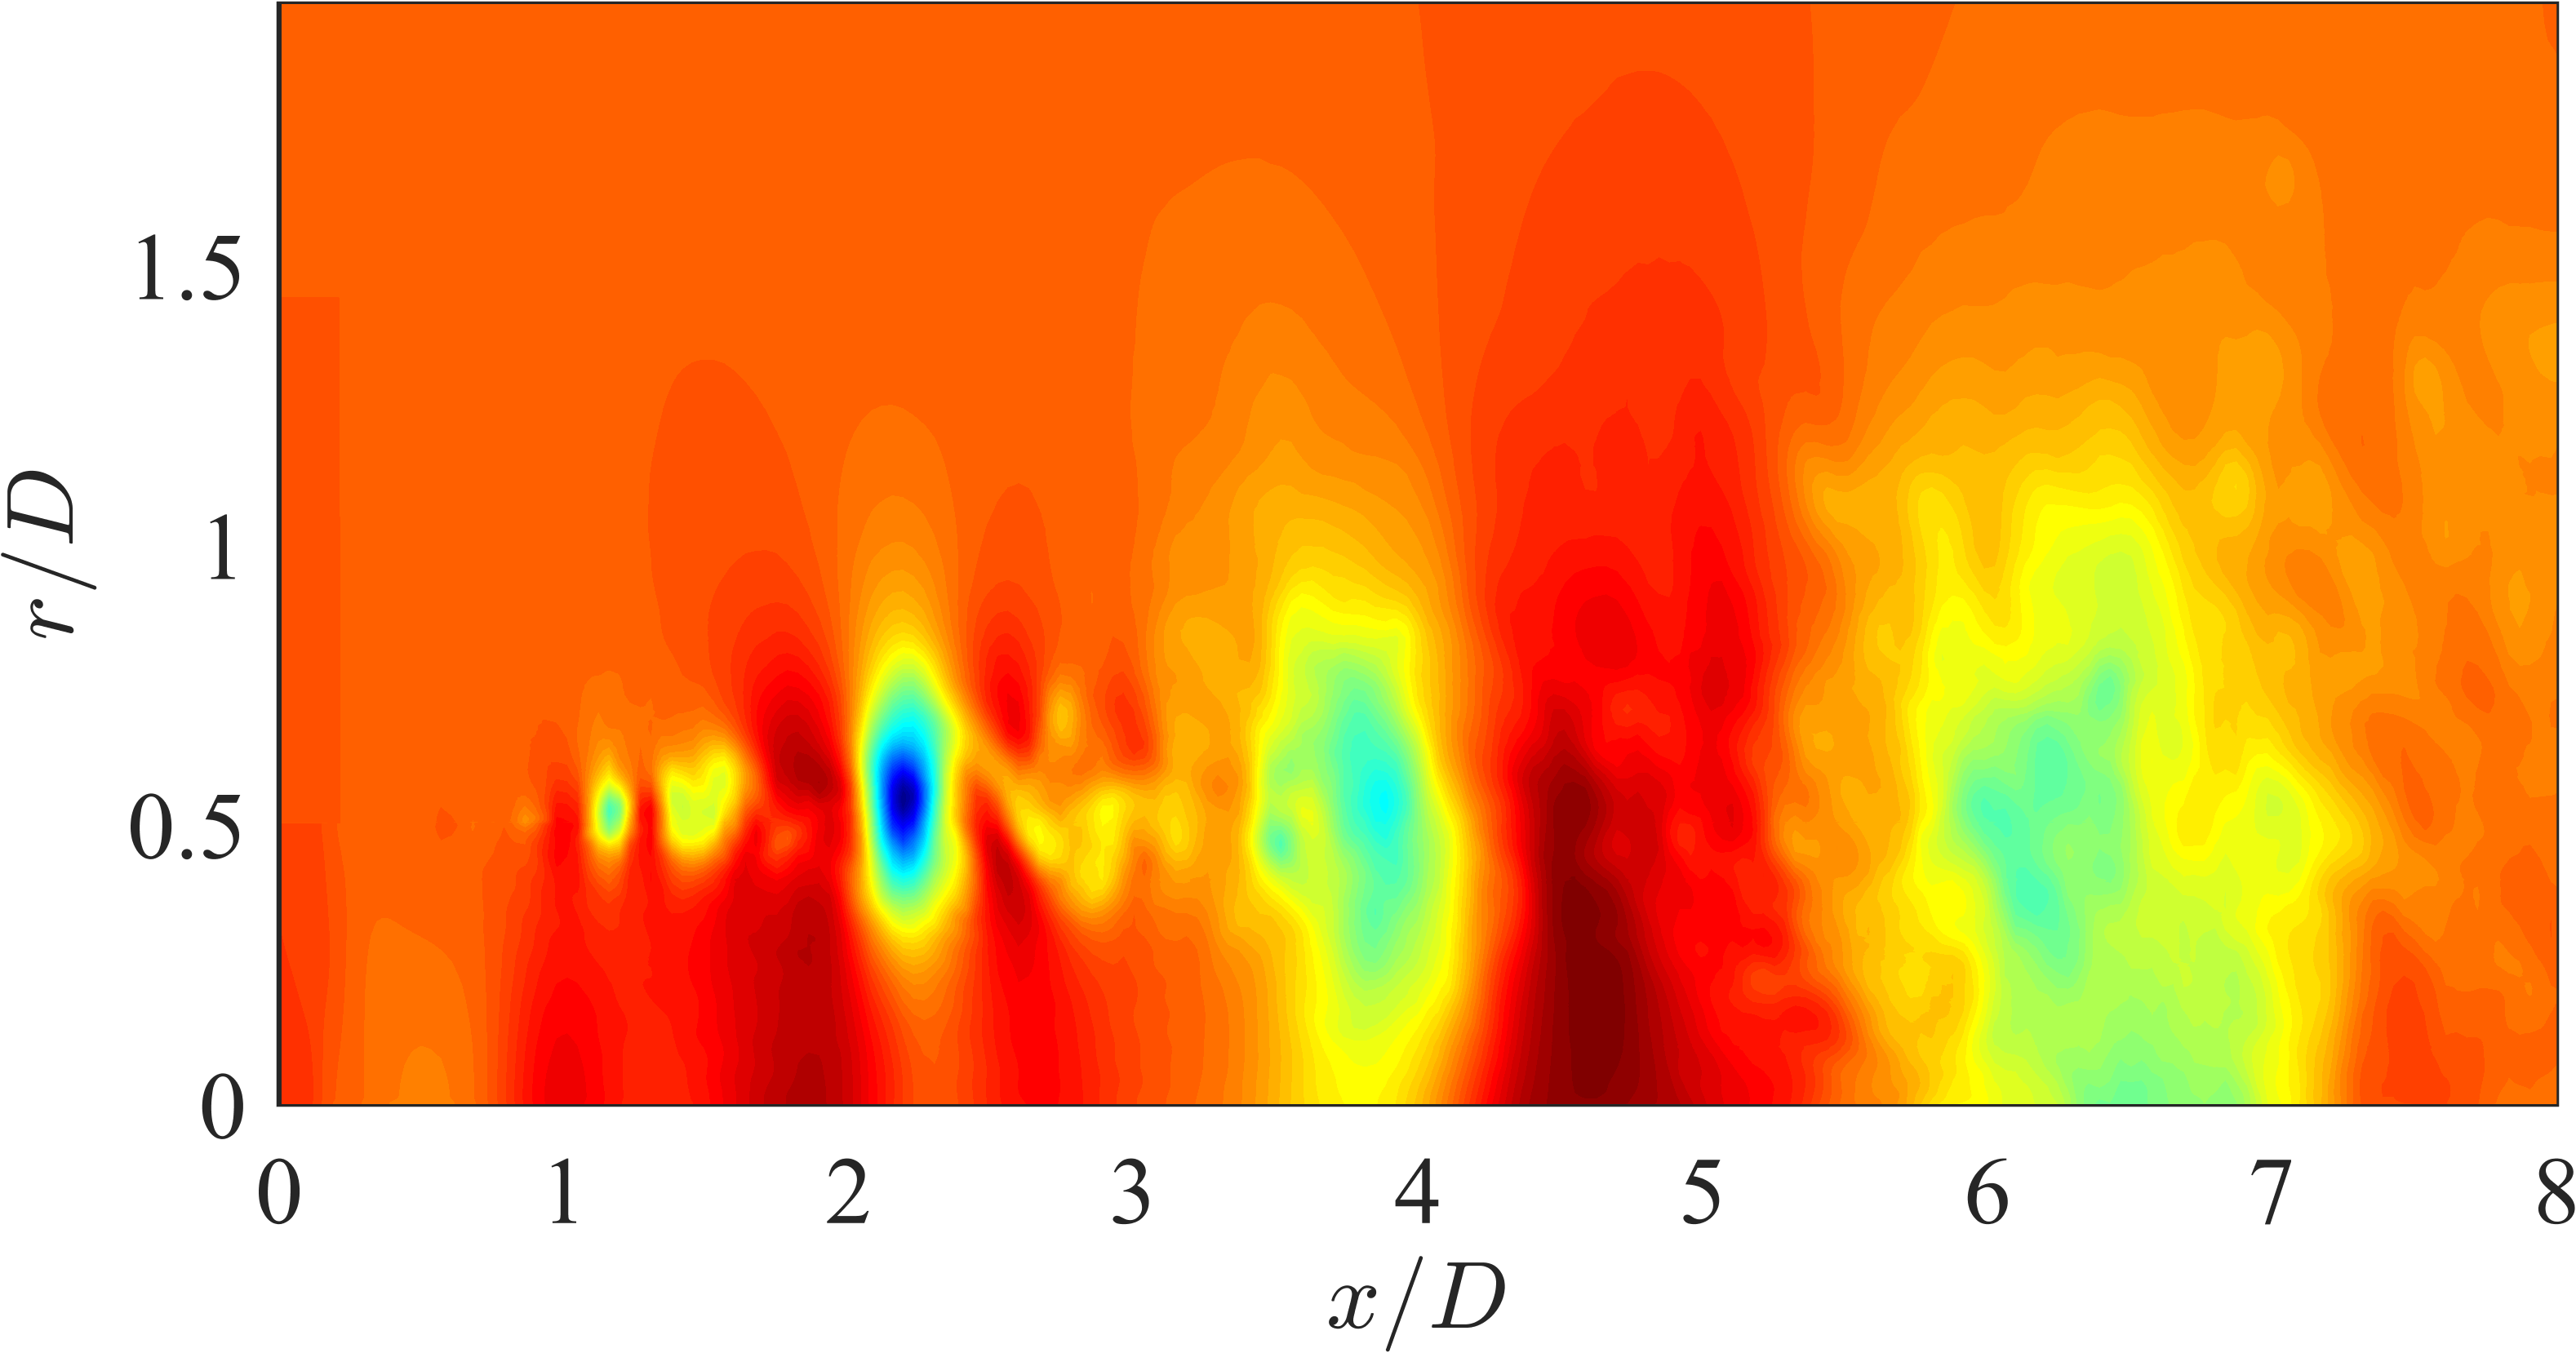
\includegraphics[width=0.6\linewidth]{Figures/LES_phavg_streamwise_p.png}
%		\caption{}
%	\end{subfigure}
	\caption{Axial velocity (a) and pressure (b) contours taken from the database of \citet{Speth2014} for $St_{DF} = 0.05$.}
	\label{fig:LES_streamwise_phavg}
\end{figure}

Though the azimuthal velocity is, unsurprisingly, non-zero, the field is highly incoherent as compared to the radial or axial velocity fields and of much lower amplitude.
The dilatation field computed using the full 3-D gradients and the partial dilatation field computed using only the radial and axial gradients can be found in \fig{fig:LES_streamwise_dil}.
Because there are weak azimuthal structures inherent even in the excited turbulent jet, a noticeable difference between the two- and full three-component dilatation fields is readily apparent in terms of fluctuation amplitude.
However, the spatial structure of the full dilatation field is largely retained in the reduced (two-component) dilatation field, just at an amplitude reduced by a nearly constant factor of $\sim 2$.
Because of this, the loss of the azimuthal gradient information is not expected to be produce unacceptable errors in the final solution.
Therefore, the azimuthal terms are dropped.
\begin{figure}
	\centering
%	\begin{subfigure}{0.75\textwidth}
%		\centering
		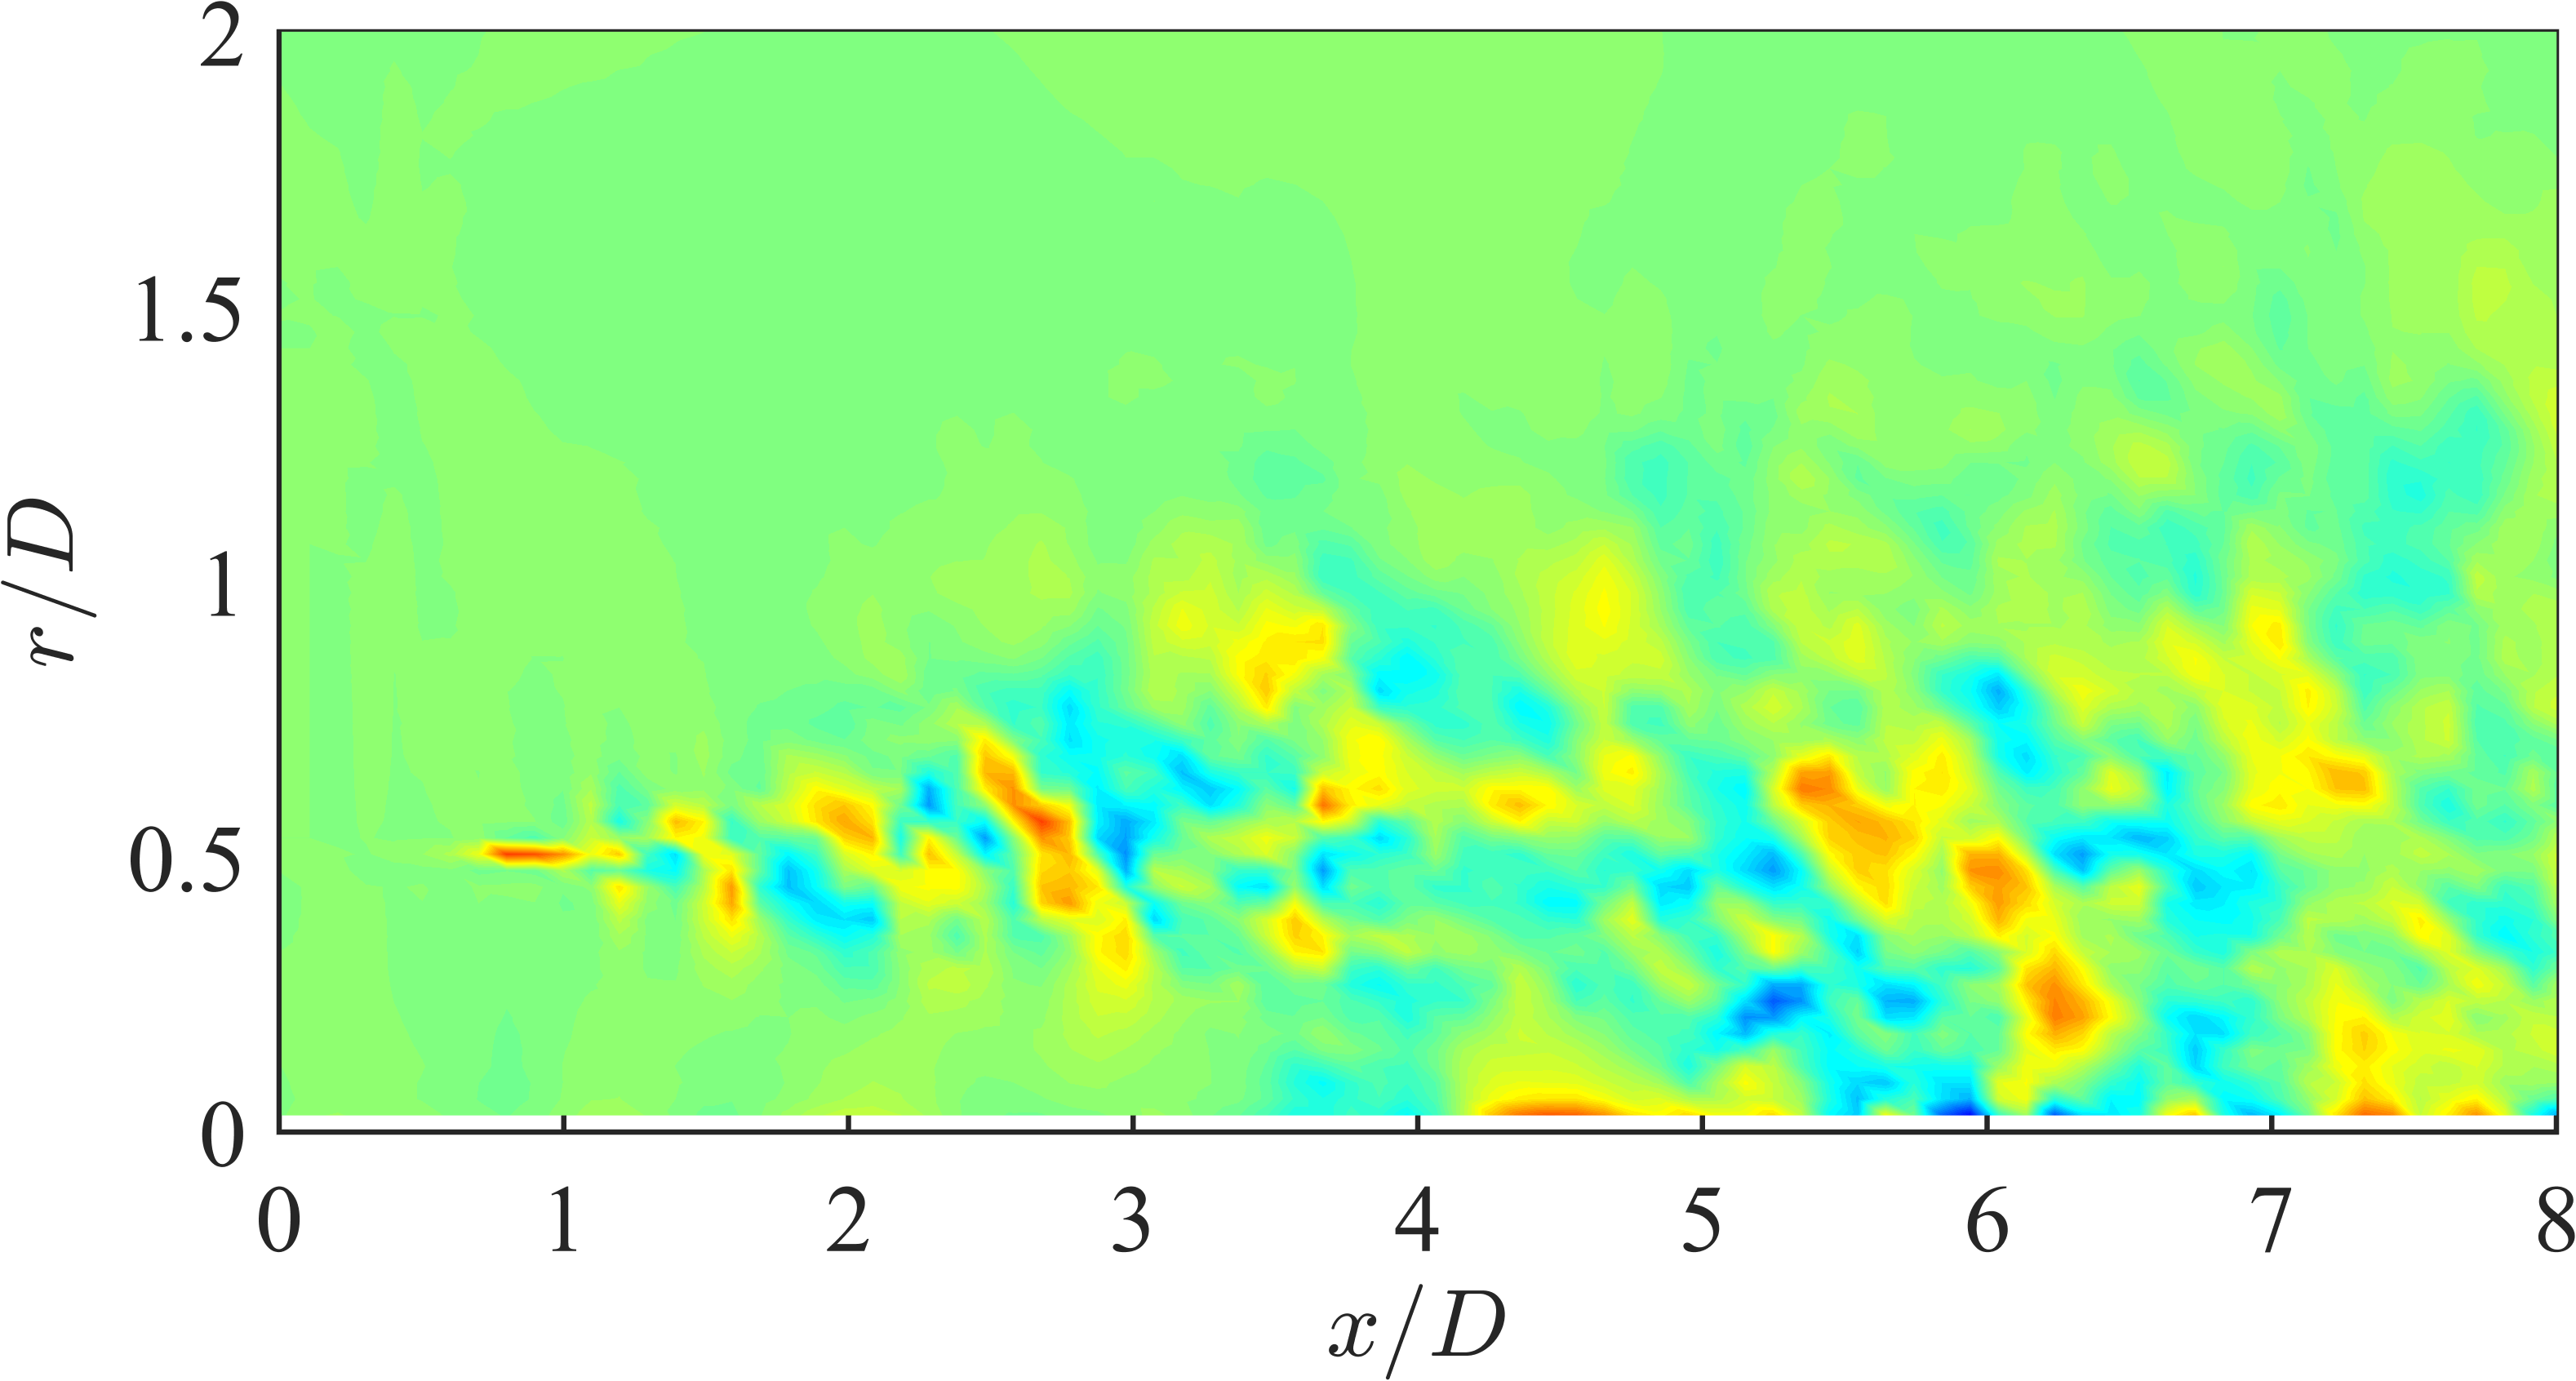
\includegraphics[width=0.6\linewidth]{Figures/LES_2CDil.png}
%		\caption{}
%	\end{subfigure}\\
%	\begin{subfigure}{0.75\textwidth}
%		\centering
		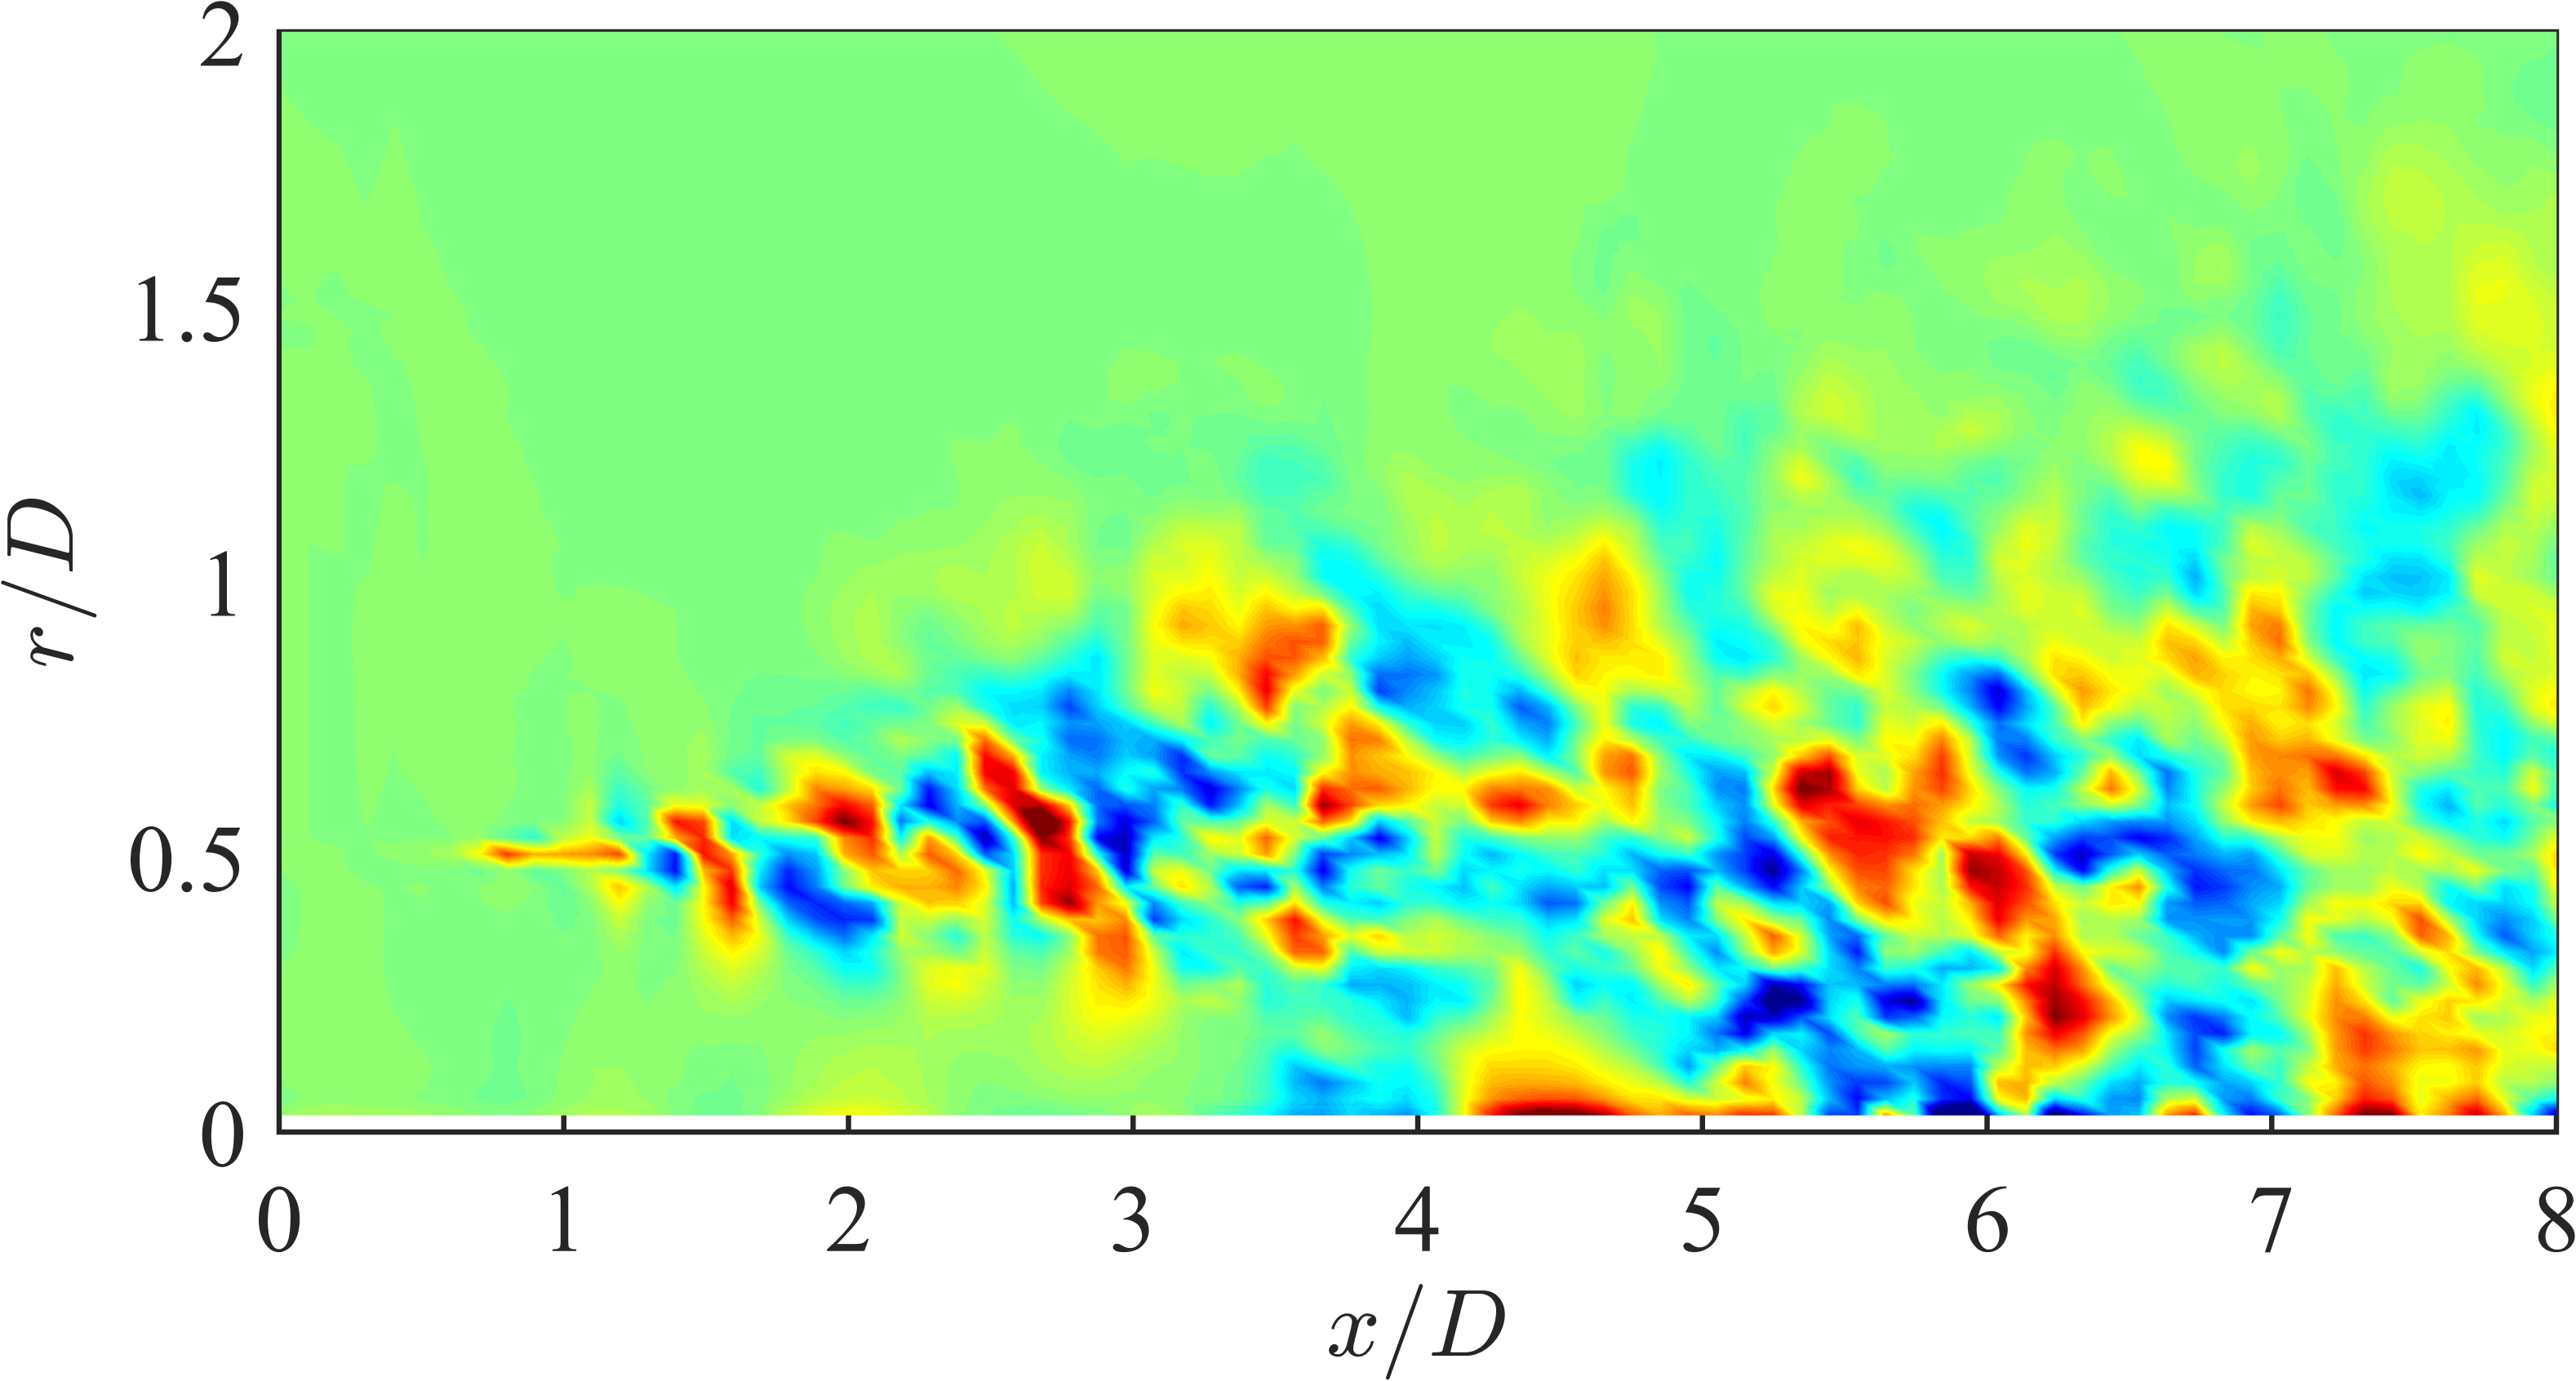
\includegraphics[width=0.6\linewidth]{Figures/LES_3CDil.png}
%		\caption{}
%	\end{subfigure}
	\caption{Dilatation computed using only the axial and radial components (a) and computed using the full three-component velocity vector (b); a uniform colorscale has been used for the two plots.}
	\label{fig:LES_streamwise_dil}
\end{figure}
 
The Helmholtz equation was solved using a standard, second-order accurate centered finite difference scheme by Taylor approximation.
A relatively low-order approximation to the spatial derivatives was deemed sufficient for this particular work, as the spatial grid was very fine compared to the wavelength of the dominant structures under investigation.
For reference, $l/ds \simeq 30$, where $l$ is the average characteristic length of the excited large-scale structures near the end of the potential core and $ds$ is the grid spacing ($ds = 0.6$ mm).
As the flow has already been assumed to be axisymmetric, only the top half-plane of the jet was used.
At the lower boundary (jet centerline), a zero-normal-gradient boundary condition was used to enforce axisymmetry.
At the radial boundary, the solenoidal component was set to zero (as there is no turbulent flow in this region, and the only outgoing waves will be compressible).
At the inflow and outflow however, the proper boundary conditions are not immediately obvious.
Other researchers using numerical databases \citep{Unnikrishnan2015} have argued that the solenoidal component be set to zero here as the turbulent eddies have either not grown to significant values or decay to insignificant values at these locations, respectively.
For the domain explored in the current work however, this does not appear to be necessarily accurate, and instead the \textit{potential} component is set to zero at both the inlet and outlet.
At the outflow boundary ($x/D \simeq 13$), there is still significant vortical behavior, but the Mach number is relatively low ($M_j \simeq 0.5$) and hence compressibility is expected to be negligible.
At the inflow boundary (which is $\sim1.4$ mm downstream of the nozzle exit), the solenoidal component is clearly not negligible in the shear layer region (since $\partial U_x / \partial r \neq 0$).
If the inflow is approximated as a plug flow (which the ensemble-averaged PIV indicates is not entirely unreasonable for the experimental grid), $\partial U_x / \partial x = \partial U_r / \partial r = 0$ and hence the potential component is negligible here.
Therefore, the potential component was set to zero at both the inlet and outlet.
Second-order accurate centered finite differences were again used to approximate the derivatives in the boundary conditions; a single ghost node was used along each boundary to enforce these conditions.

Sample results from the experimental database for this procedure have been provided in \fig{fig:valid_helmholtz}.
Here, the axial and radial velocity components for the original (estimated) and decomposed velocity fields are shown for $St_{DF}=0.05$.
From the raw velocity field, a single large-scale structure is readily identifiable at $x/D \simeq 6$ (which is the end of the potential core).
Due to the very low frequency of the excitation (impulsive forcing), no other large-scale structures are clearly visible in the flow-field.
As expected, the Helmholtz decomposition produces a solenoidal velocity that is quite similar to the full velocity field; even at high subsonic Mach numbers, compressibility plays a minor (though definitely non-negligible) role in the overall evolution of the shear layer and potential core.
The upstream development of the potential field, in which no large-amplitude oscillations are observed, validates the assumption of plug flow made in the boundary conditions.
In contrast, non-negligible fluctuations are observed near the outflow boundary; unfortunately, the experimental domain does not extend far enough downstream for the compressible component to fully decay.
However, the potential component is still far weaker than the solenoidal component.
For validation purposes, the boundary conditions of \citet{Unnikrishnan2015} (zero solenoidal component at the inflow and outflow) were also implemented and compared against the current results.
Though not shown here for brevity, the zero-solenoidal boundary conditions produced similar fields at the interior of the domain, but non-physical oscillations at the inflow and outflow boundaries.
Based on these results, the zero-potential boundary conditions were retained; though there is a discrepancy between the boundary conditions and the physical system at the outflow boundary, the numerical effects of this are expected to be minor.
\begin{figure}
	\centering
%	\begin{subfigure}{0.5\textwidth}
%		\centering
		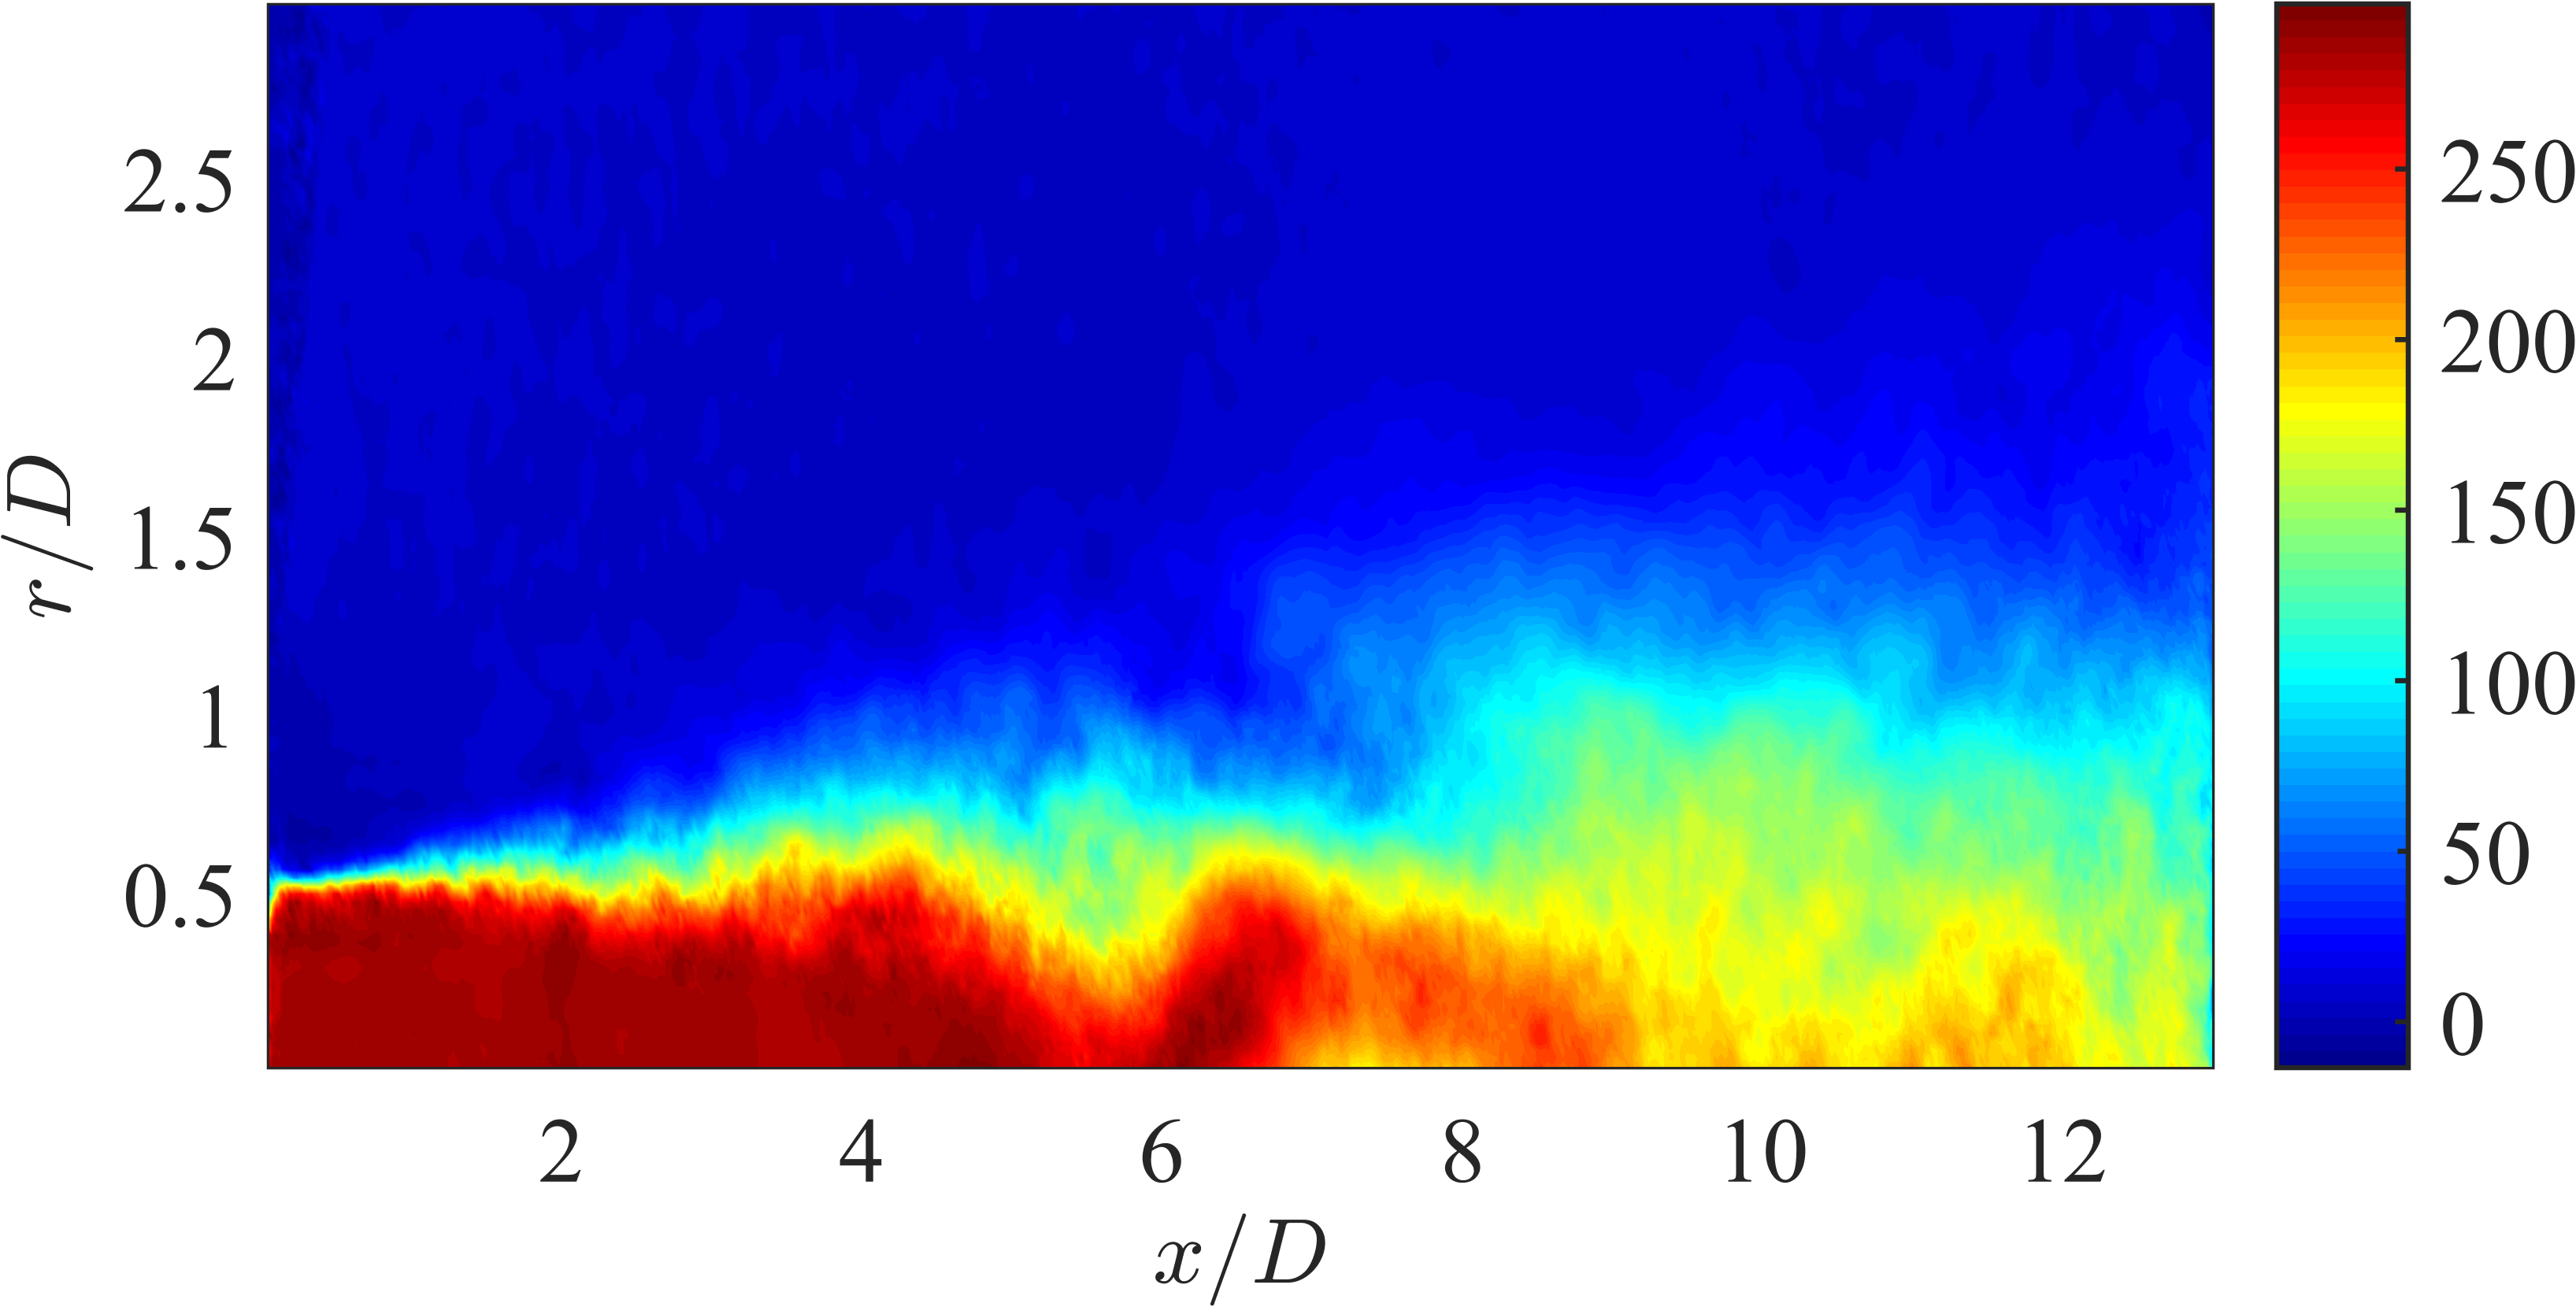
\includegraphics[width=0.45\linewidth]{Figures/ch5_valid_Inst_Uz.png} %
%		\caption{}
%	\end{subfigure}%
%	\begin{subfigure}{0.5\textwidth}
%		\centering
		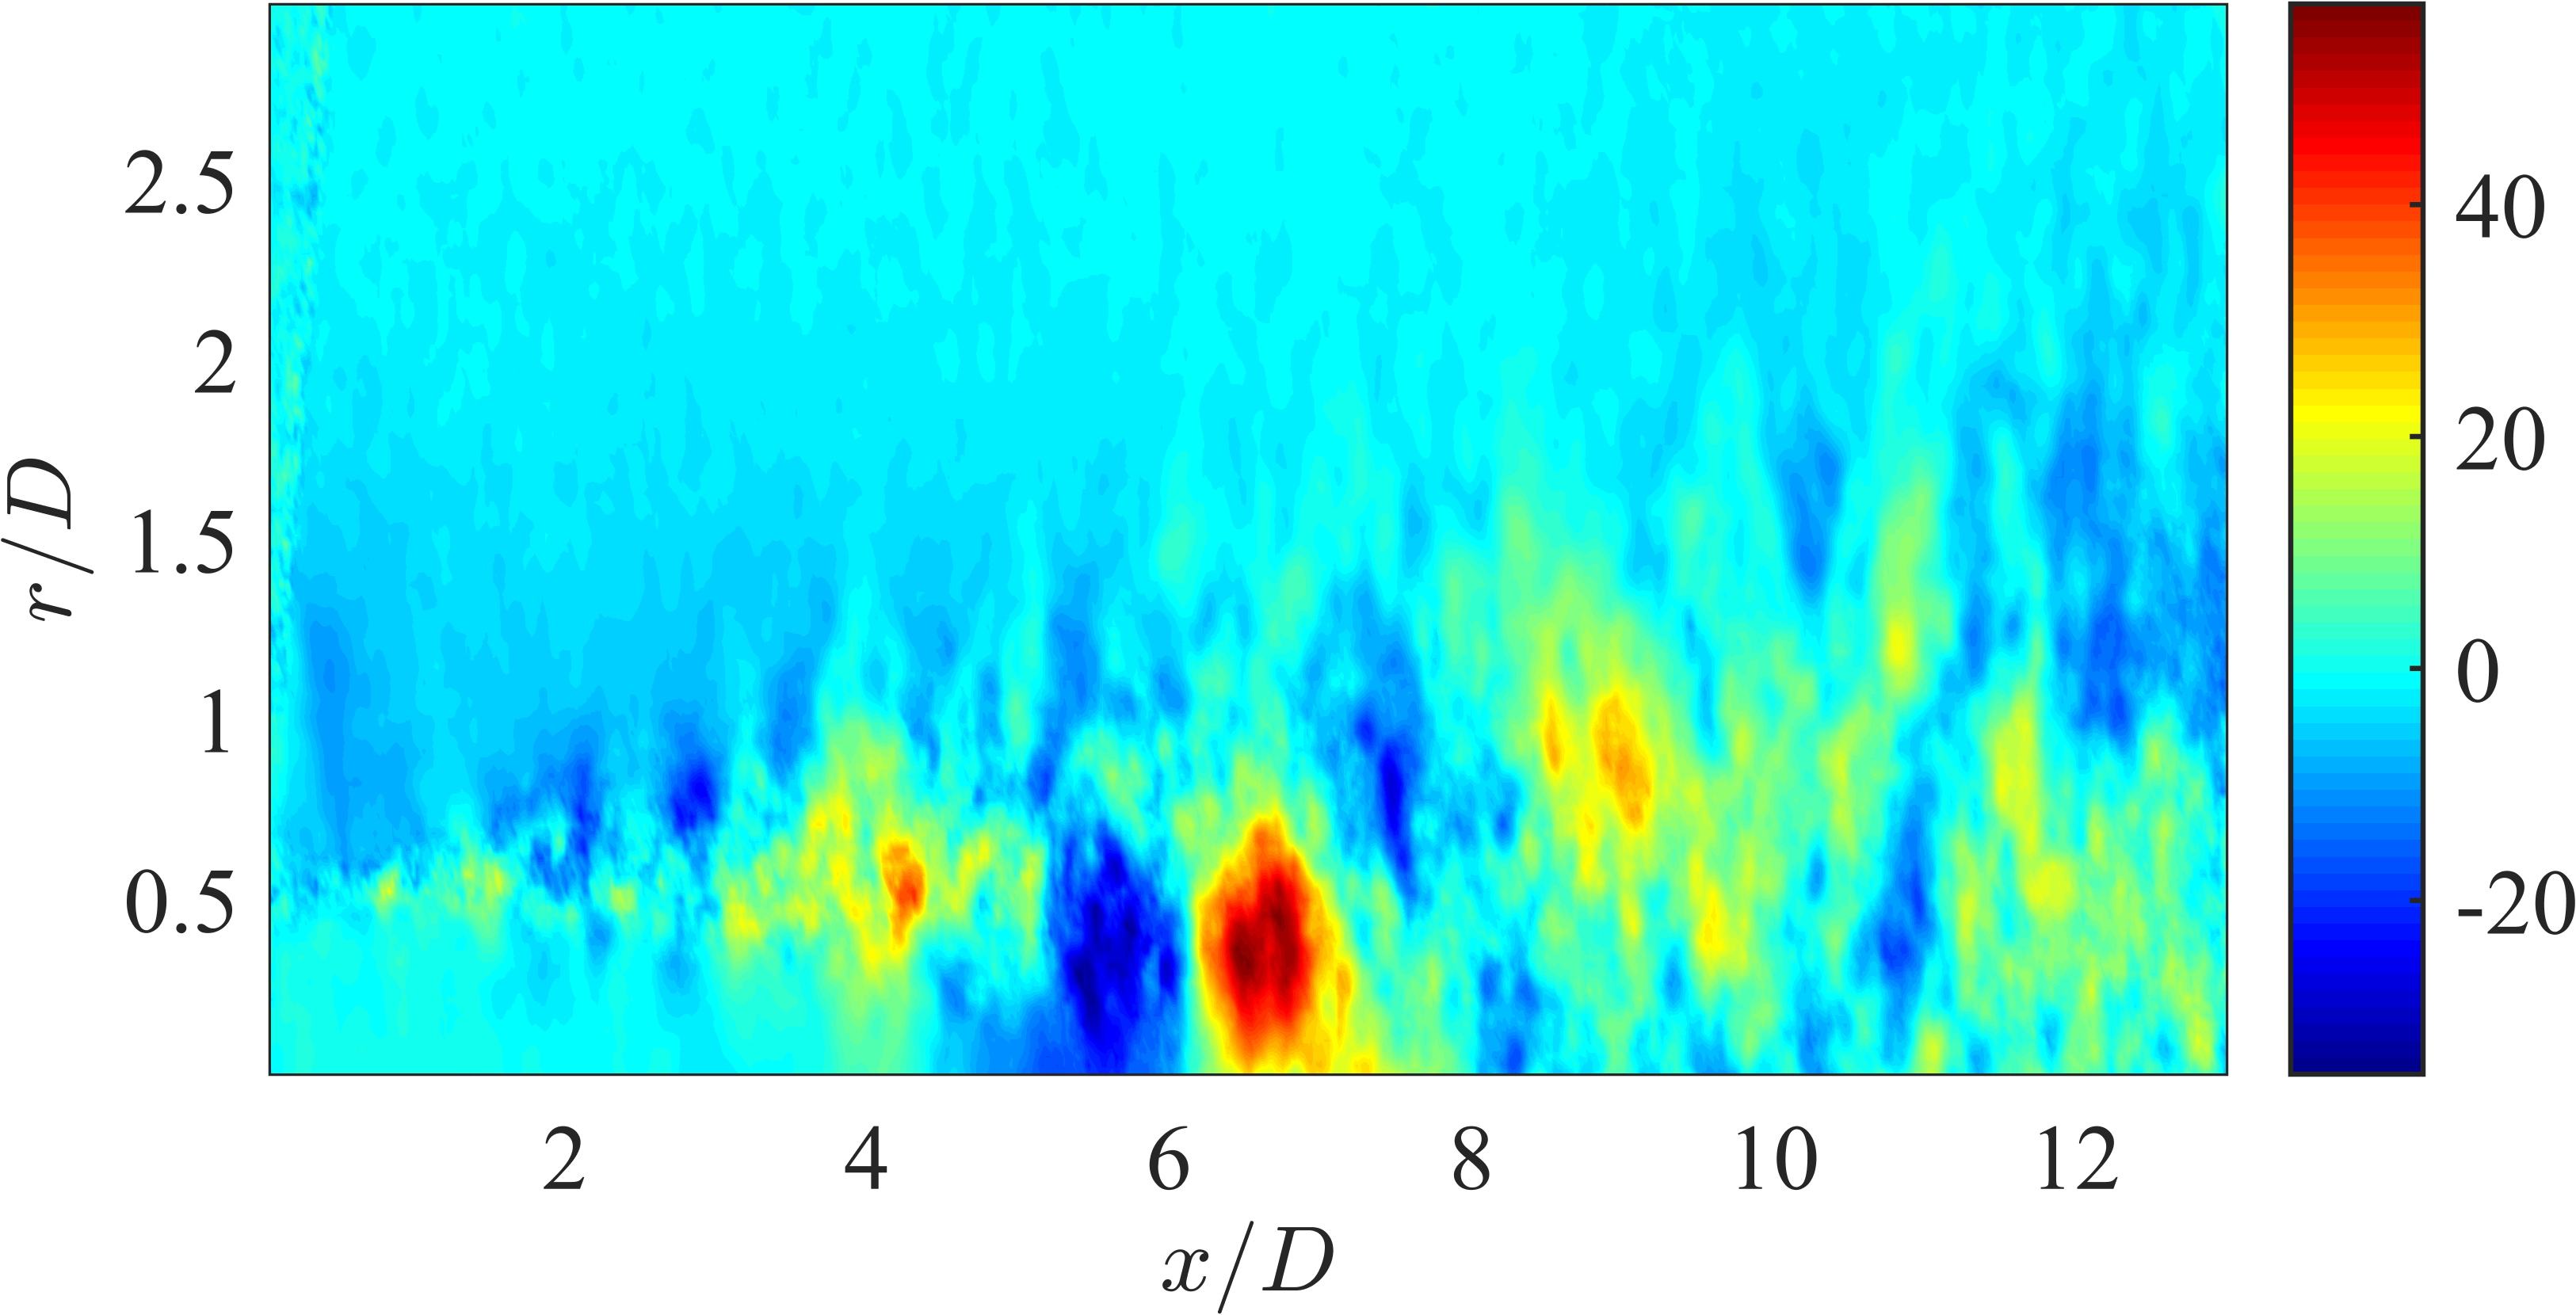
\includegraphics[width=0.45\linewidth]{Figures/ch5_valid_Inst_Ur.png}\\
%		\caption{}
%	\end{subfigure}\\
%	\begin{subfigure}{0.5\textwidth}
%		\centering
		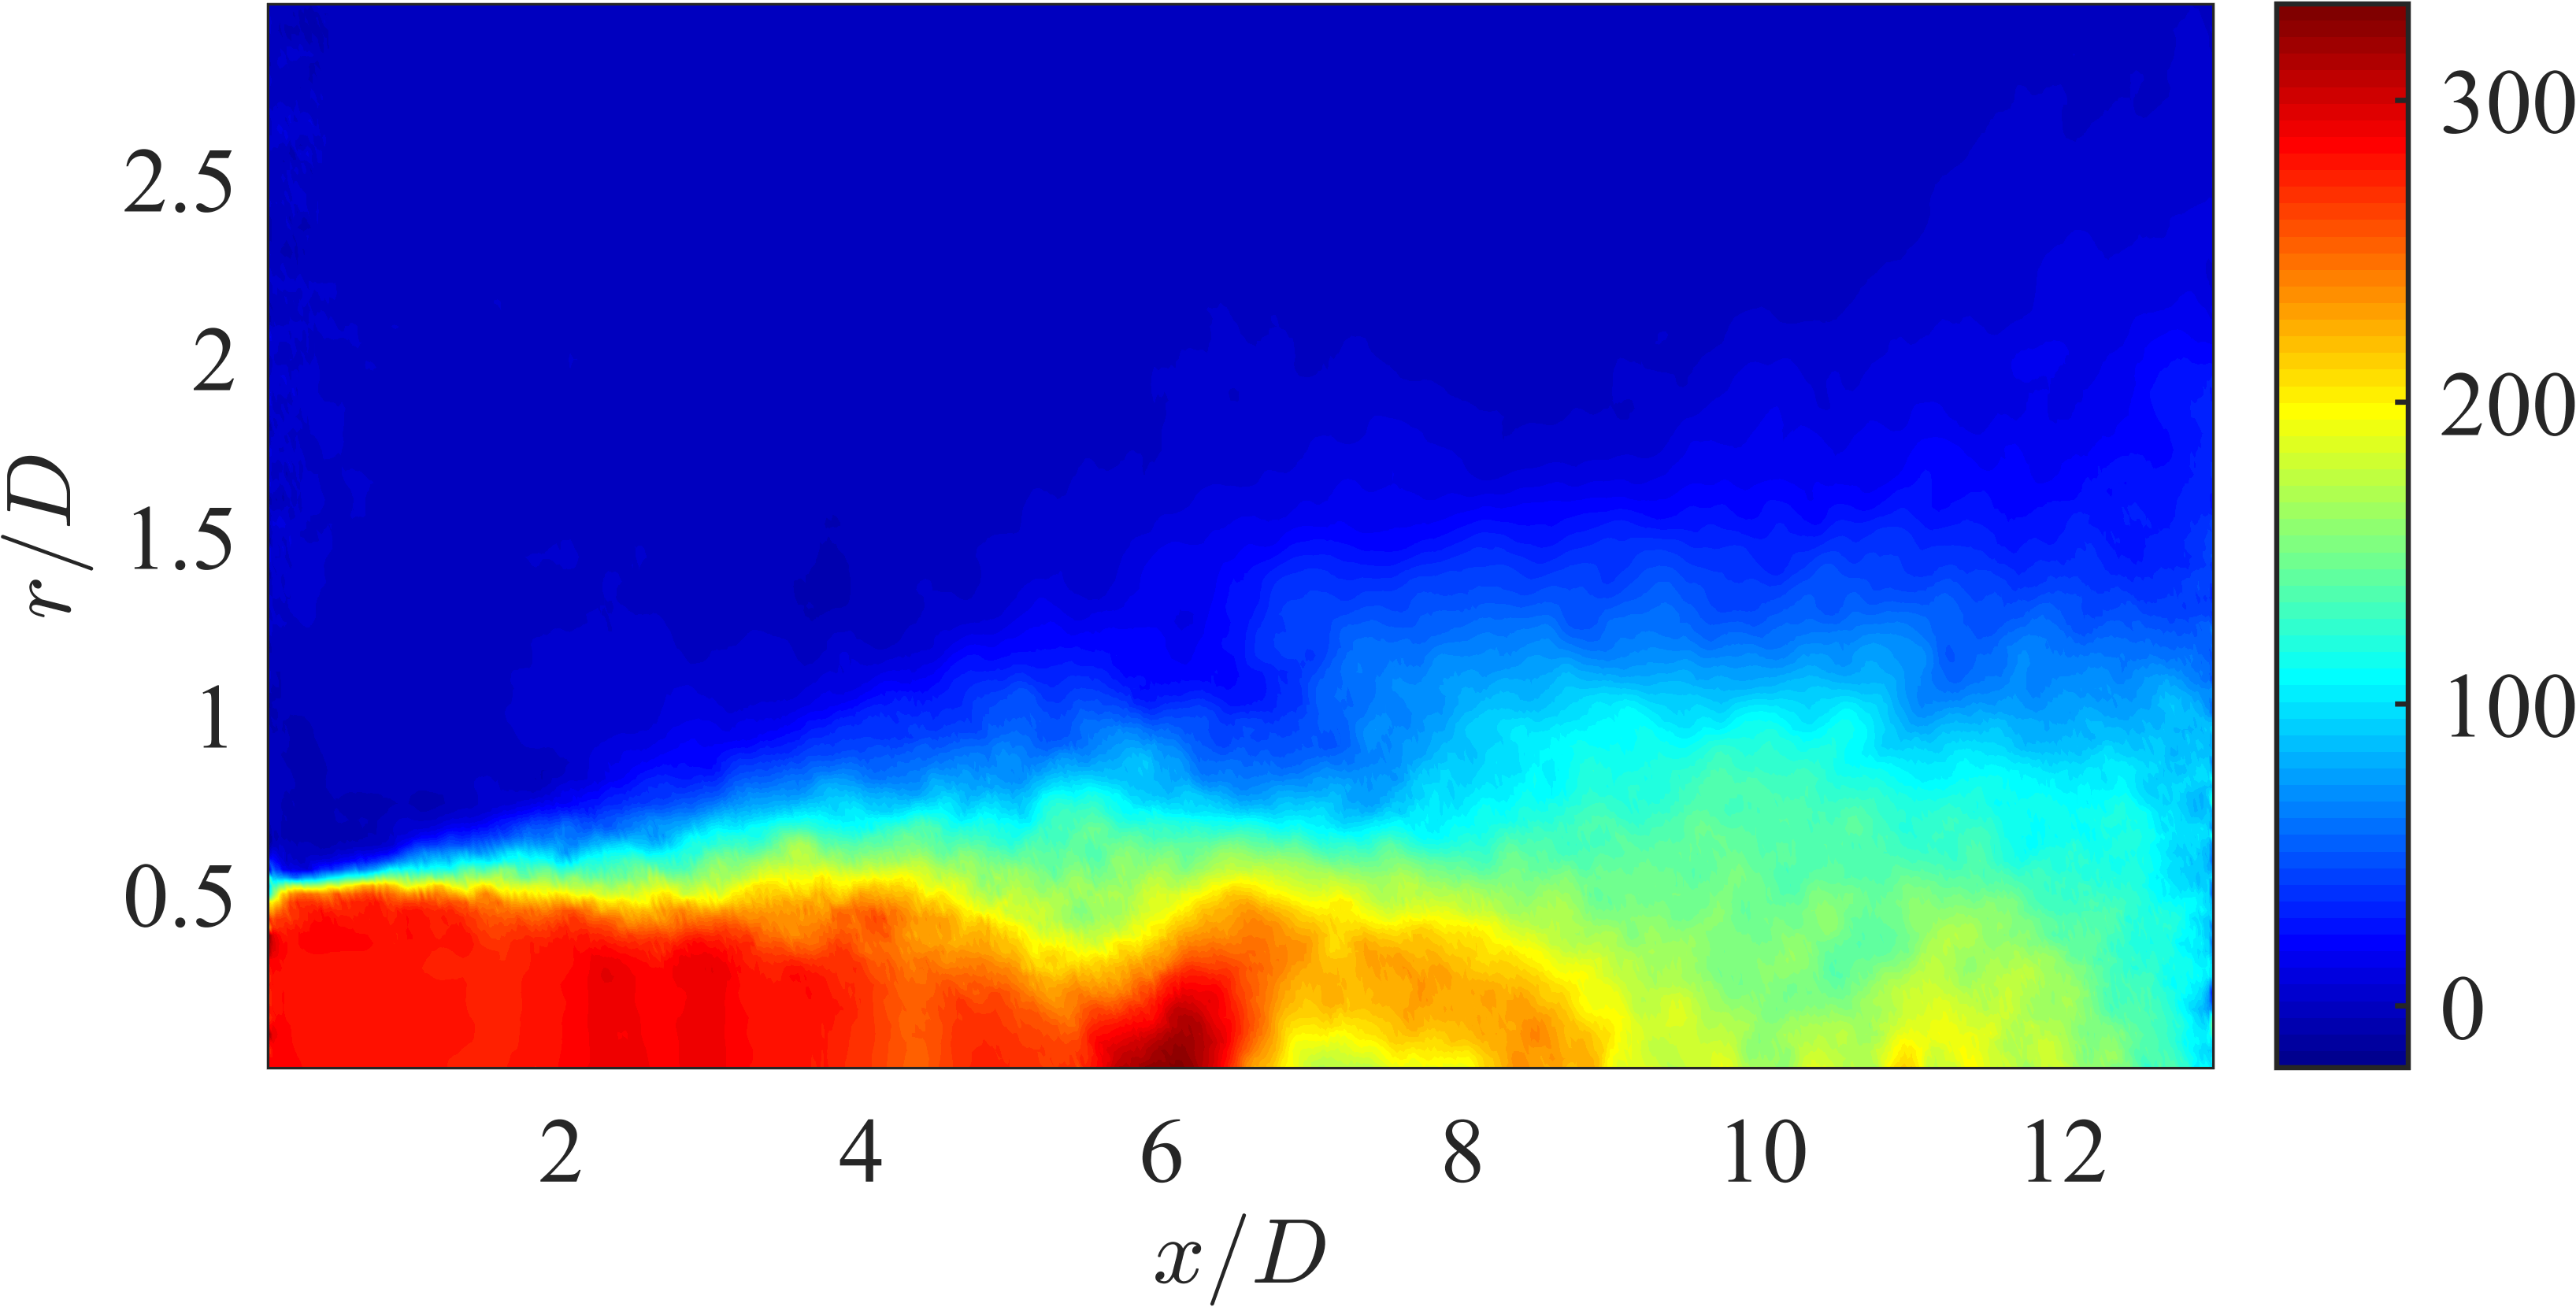
\includegraphics[width=0.45\linewidth]{Figures/ch5_valid_Inst_solUz.png}
%		\caption{}
%	\end{subfigure}%
%	\begin{subfigure}{0.5\textwidth}
%		\centering
		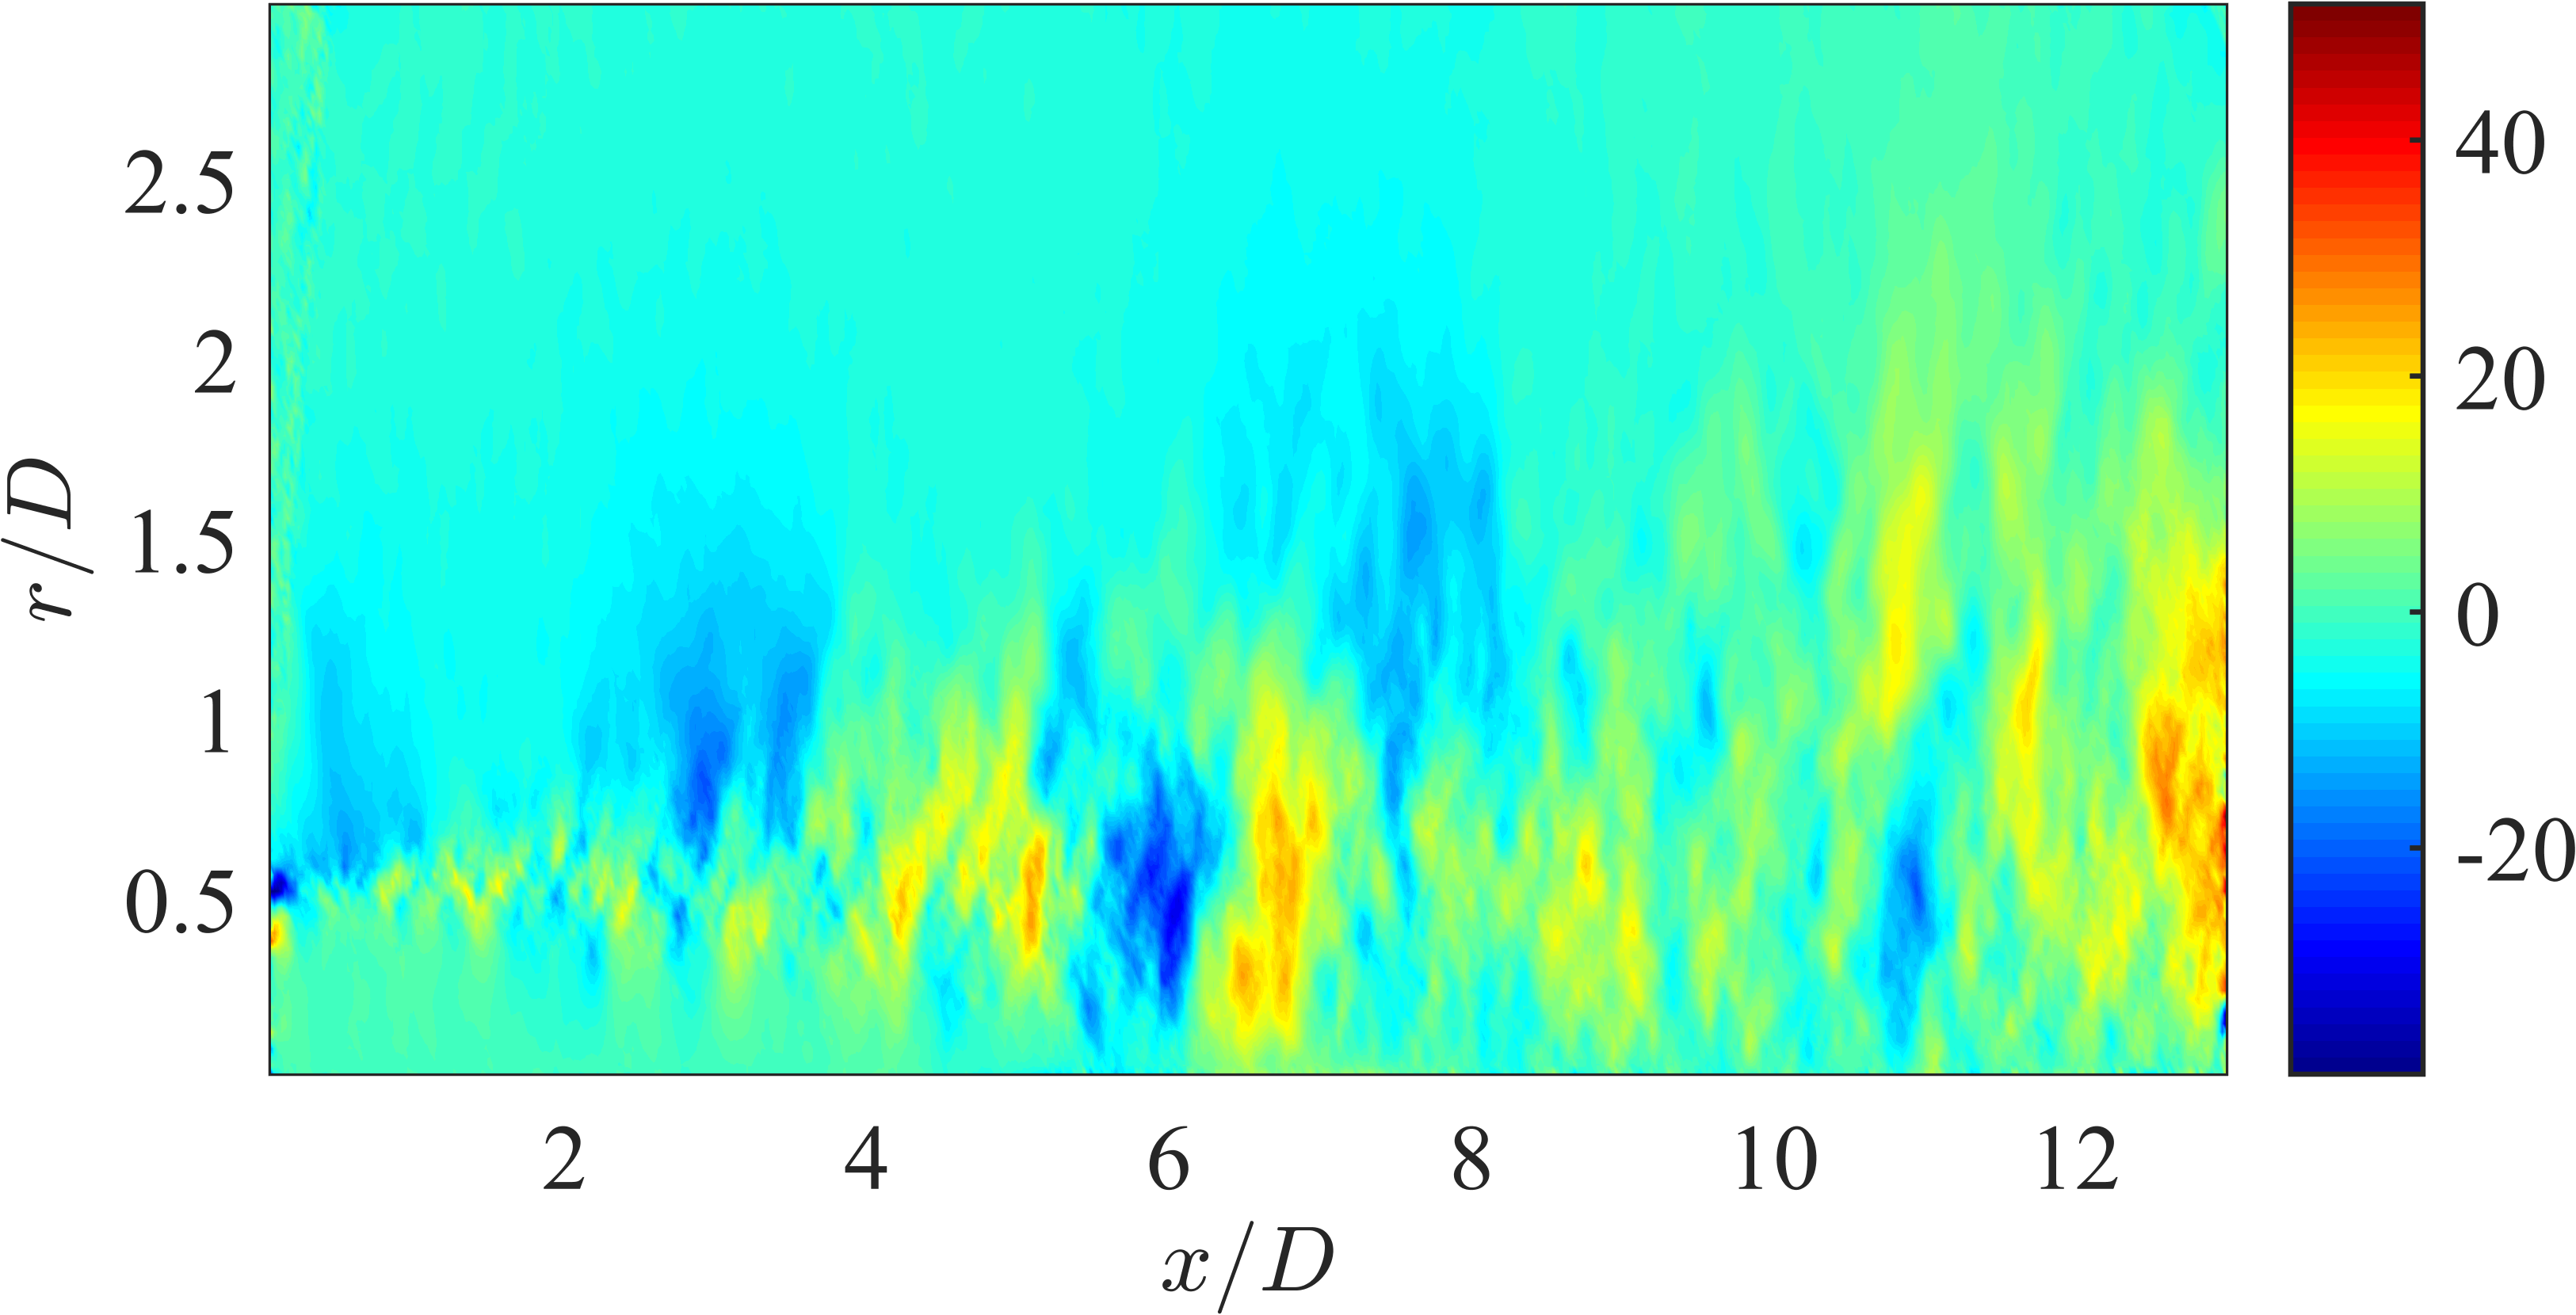
\includegraphics[width=0.45\linewidth]{Figures/ch5_valid_Inst_solUr.png}\\
%		\caption{}
%	\end{subfigure}\\
%	\begin{subfigure}{0.5\textwidth}
%		\centering
		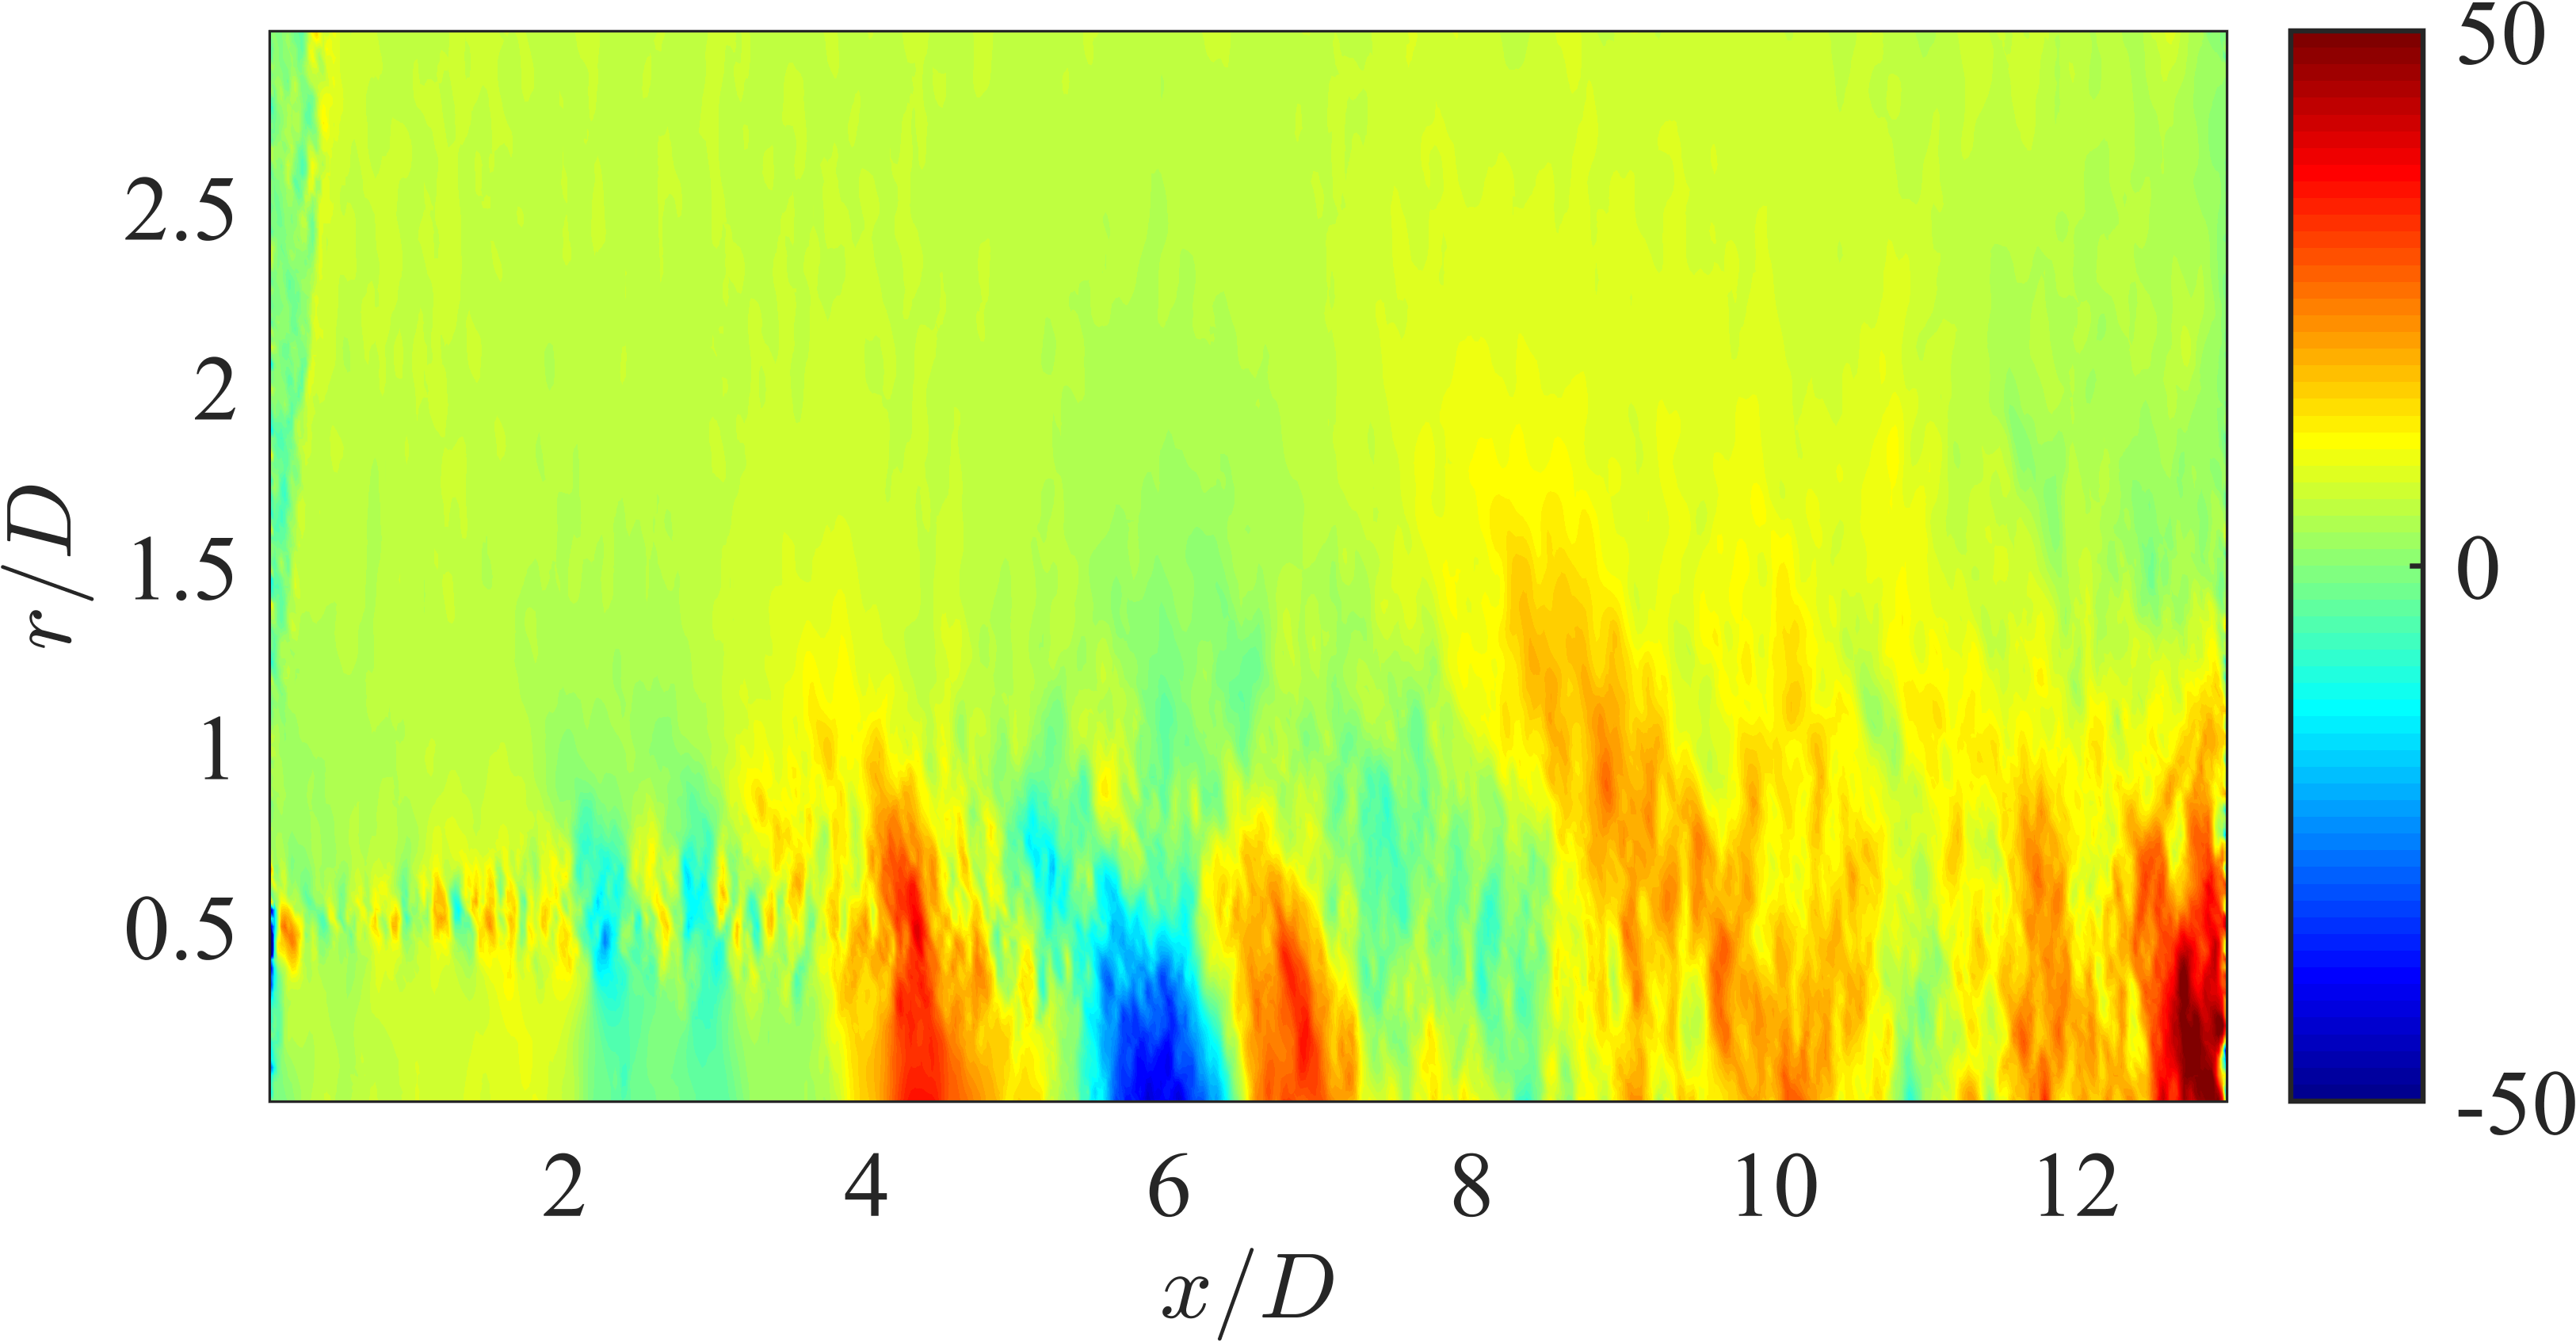
\includegraphics[width=0.45\linewidth]{Figures/ch5_valid_Inst_potUz.png}
%		\caption{}
%	\end{subfigure}%
%	\begin{subfigure}{0.5\textwidth}
%		\centering
		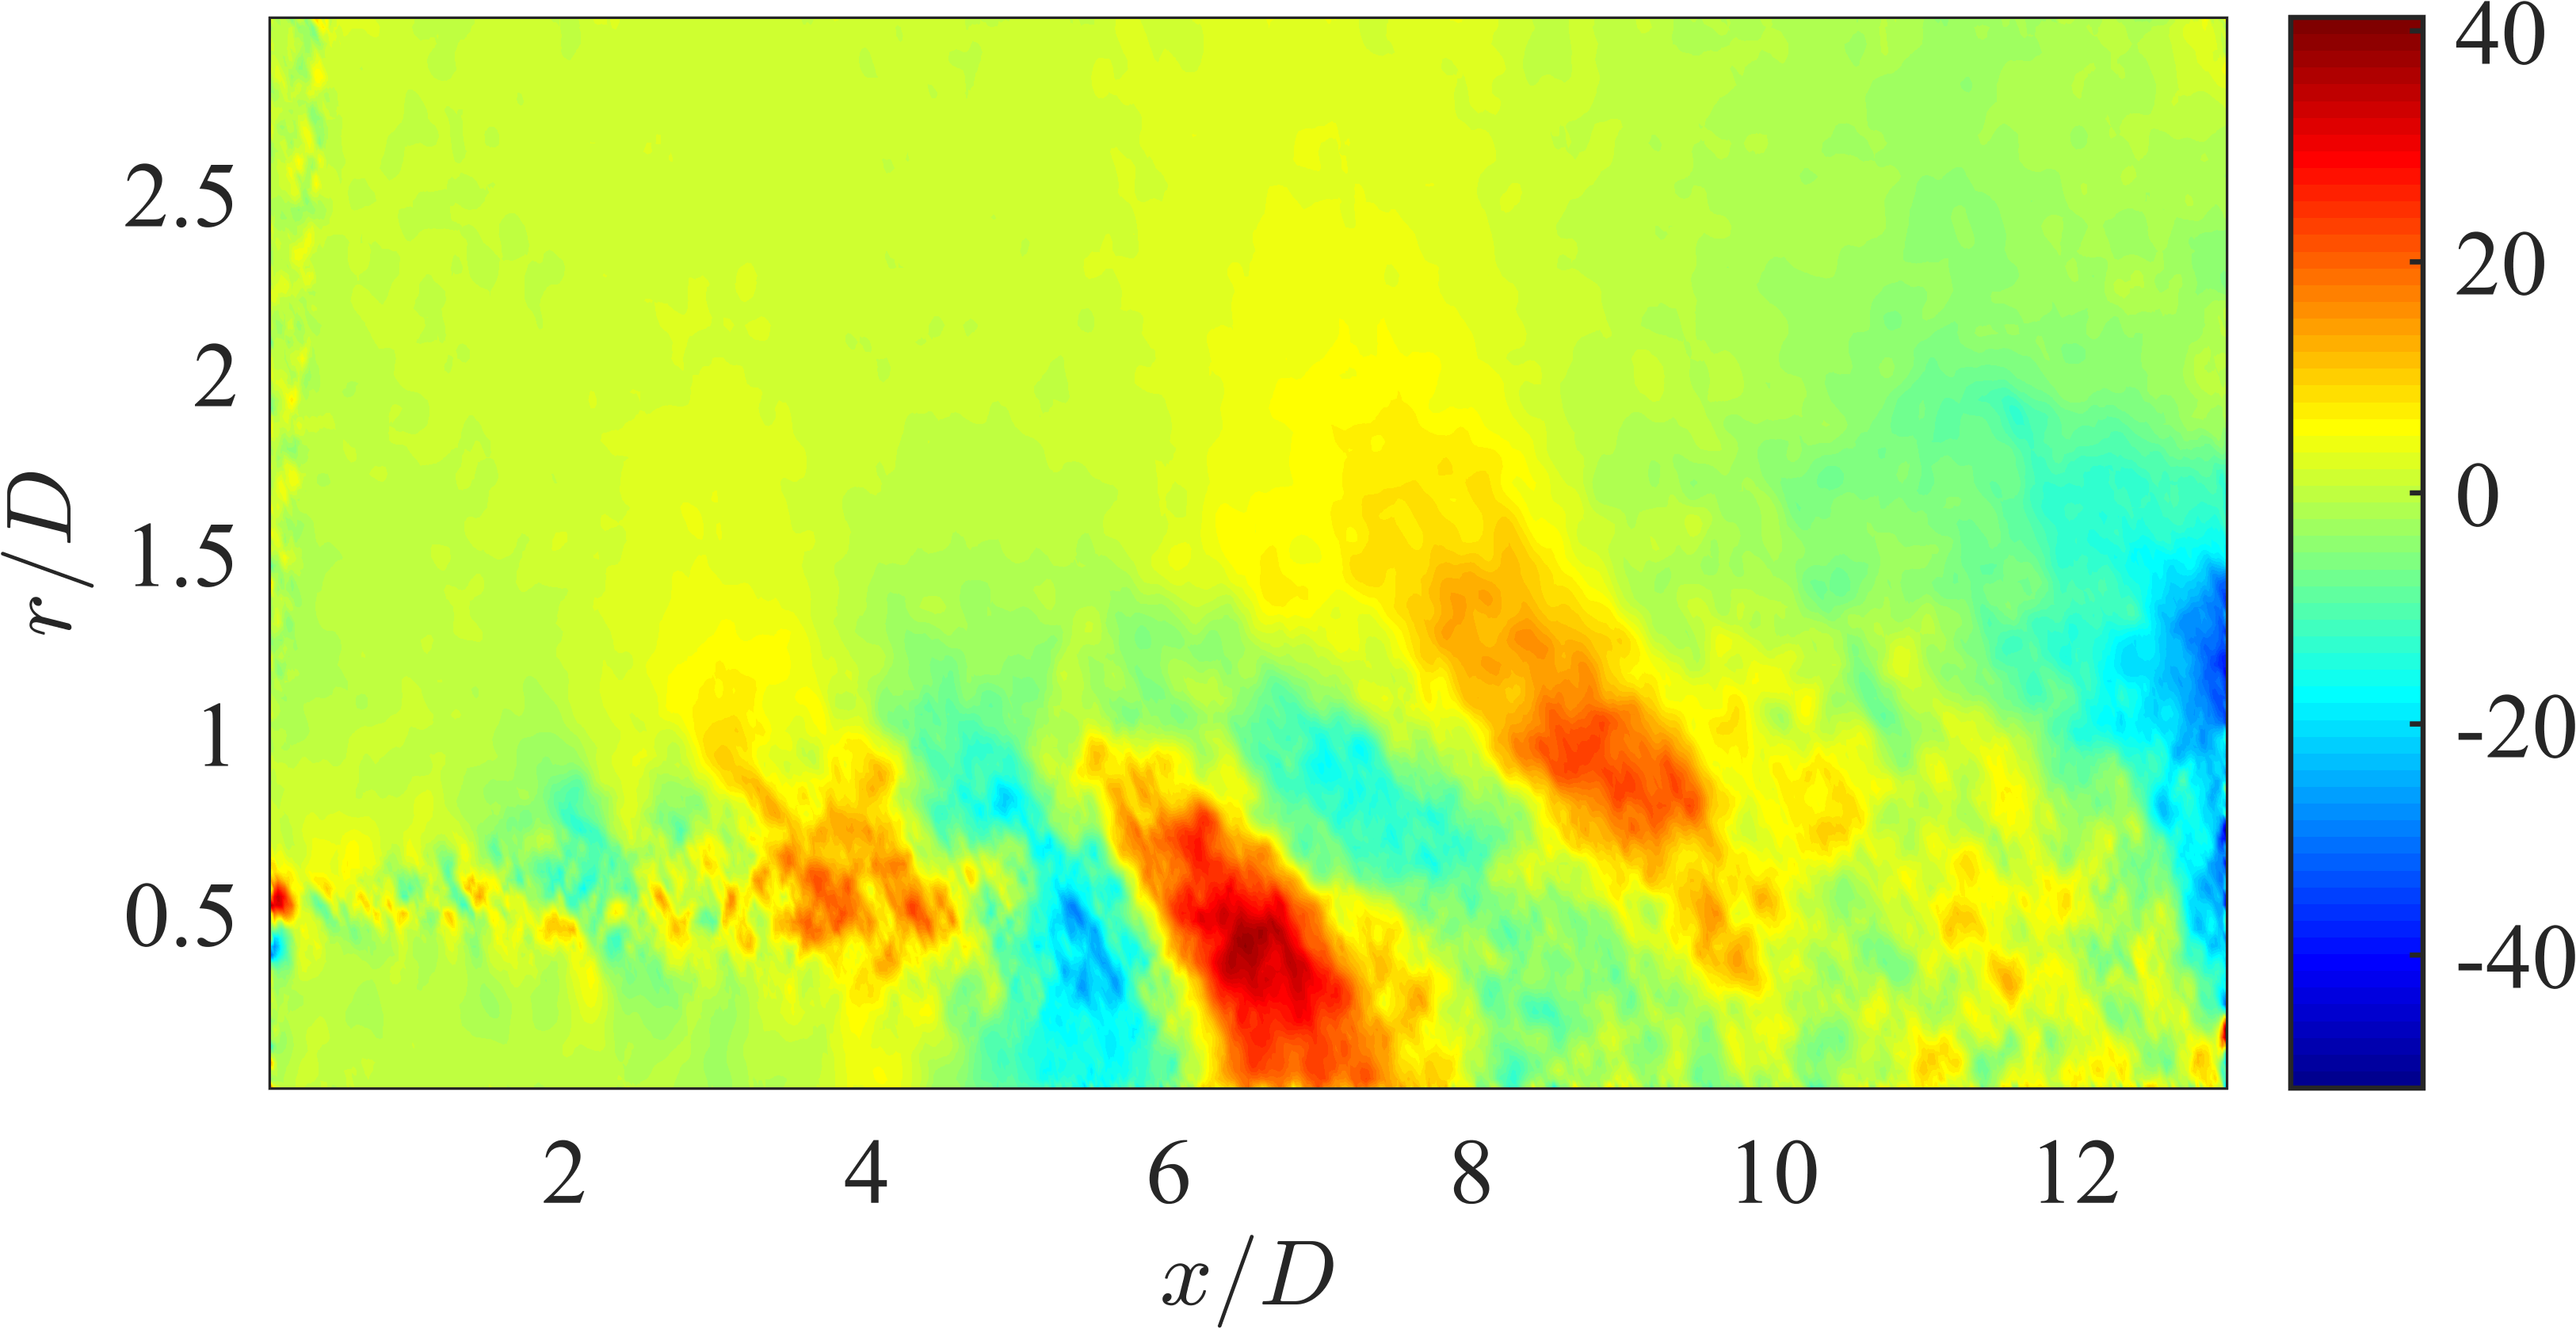
\includegraphics[width=0.45\linewidth]{Figures/ch5_valid_Inst_potUr.png}
%		\caption{}
%	\end{subfigure}
	\caption{Instantaneous axial (a,c,e) and radial (b,d,f) velocity components for the original (a,b), solenoidal (c,d), and potential (e,f) velocity fields (units in m/s), for $St_{DF} = 0.05.$}
	\label{fig:valid_helmholtz}
\end{figure}

\subsubsection{Pseudo-Pressure Solver}
Once the solenoidal velocity field is known, the fluctuating pseudo-sound field can be computed as the incompressible solution to the momentum and continuity equations.
The source field is calculated explicitly from the solution of the Helmholtz decomposition (that is, the double divergence of the incompressible velocity stress tensor) using second-order accurate finite differences.
As with the preceding Poisson equation, the azimuthal terms in this second Poisson equation are assumed negligible in comparison to the radial and axial terms and are thus ignored.
Again, as done previously for the Helmholtz decomposition, the governing equation is approximated using second-order accurate centered finite differences, and ghost nodes are used at the domain boundaries to enforce the boundary conditions.

The hydrodynamic pressure field has been observed to strongly decay with radial position \citep{Arndt1997}; given the radial extent of the experimental domain, it was therefore assumed that the pseudo-sound fluctuations have decayed to negligible values by the time they reach the upper domain boundary.
In accordance with the boundary assumptions made in the preceding section, at the inflow boundary plug flow has again been assumed, meaning that the pseudo-pressure \textit{fluctuations} are negligible at the inlet. 
The outflow boundary was assumed to be far enough downstream such that the fluctuations were also negligible at the boundary.
Finally, the lower boundary enforced the zero-normal-gradient required by the assumption of axisymmetry.

Sample results for the pseudo-pressure field are shown in \fig{fig:valid_pseudopressure}, which corresponds to the solenoidal velocity decomposed in \fig{fig:valid_helmholtz}.
As expected, a spatially-coherent fluctuation is observed coinciding with the location of the large-scale structure as identified in the velocity field.
Lower-amplitude oscillations are also observed upstream of the end of the potential core, while downstream the fluctuations are fairly incoherent and low-amplitude.
By the end of the experimental domain, the pseudo-pressure field has decayed to essentially negligible values.
At the inlet however, a large-amplitude pressure sink resides along the jet lipline and extends for $x/D \lesssim 0.5$.
The origin of this pressure sink is not clear to the researcher, however it is entirely numerical in nature; as will be seen in the following section, the consistency of this sink results in no superfluous aeroacoustic source being computed for this location.
While the presence of this numerical error is unfortunate, given that it was not found to have a major effect on the computed aeroacoustic source field (which is ultimately the goal of this analysis), further inquiry into the cause of this numerical error was deemed unproductive.
\begin{figure}
	\centering
	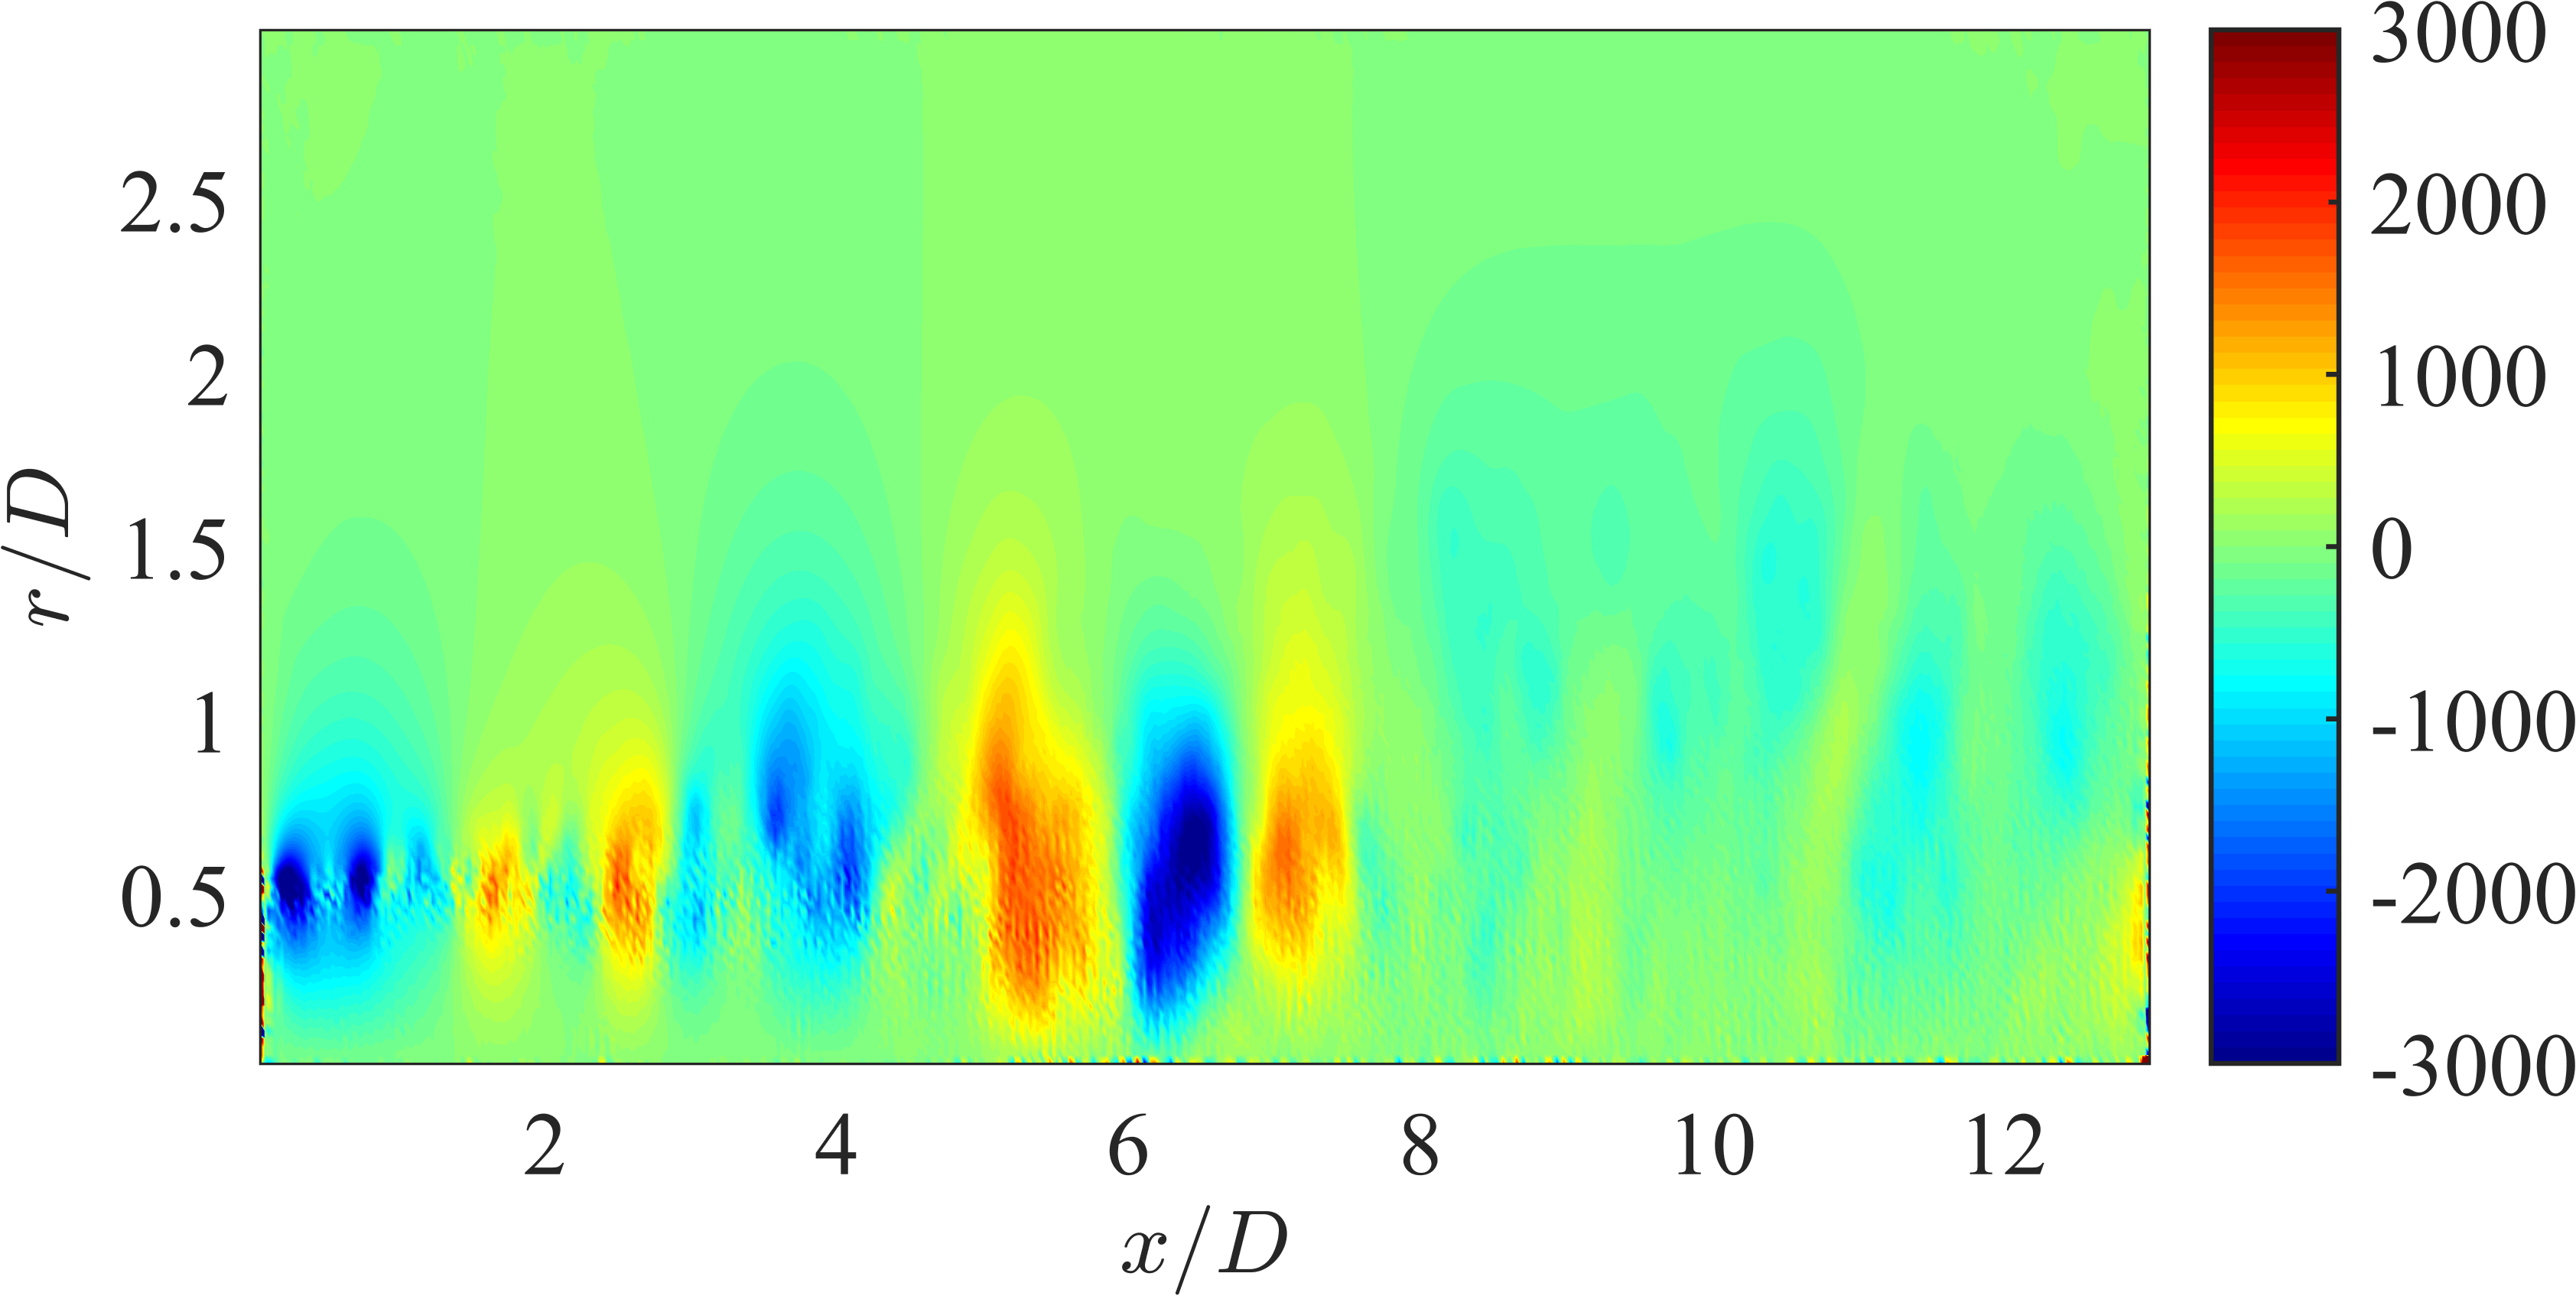
\includegraphics[width = 3.5in]{Figures/ch5_valid_Inst_ps.png}
	\caption{Instantaneous pseudo-pressure field for the same conditions as \fig{fig:valid_helmholtz}.}
	\label{fig:valid_pseudopressure}
\end{figure}

\subsubsection{Aeroacoustic Source}
The aeroacoustic source term can now be computed explicitly as the second temporal derivative of the pseudo-sound field (\eq{eq:ribner_source}).
However, filtering of the pseudo-pressure field along the temporal dimension was found to be necessary before computation of the derivative, due to the accumulation of experimental and numerical error.
Wavelet-based filtering was chosen to remove the influence of the experimental/numerical errors; an energy threshold was applied to the orthogonal wavelet coefficients in order to remove the less-energetic, incoherent events from the pseudo-pressure field.
For the current work, the fast orthogonal wavelet transforms implemented in Stanford University, Department of Statistics' \texttt{WaveLab 850} software library were utilized.
The mother wavelet was defined as the $5^{th}$-order Battle-Lemarie wavelet; sample data was also analyzed using other smooth wavelets to ensure that the final results were not affected by the choice of mother wavelet.
A threshold of $\epsilon = 8 \sigma_n \sqrt{ \mathrm{log}_e N}$ was used; this value was found by trial-and-error to be the lowest threshold which consistently removed all discontinuities in the temporal derivative of the pressure trace.

Once the pseudo-pressure field has been properly filtered, the aeroacoustic source is simply calculated using second-order finite differences in time (\fig{fig:valid_denoising}).
To compute the far-field noise, the source field can be spatially-integrated in retarded time, accounting for the propagation delay from each source location to the observer, per \eq{eq:source_integration}; here, this was performed by trapezoidal integration. 
\begin{figure}
	\centering
	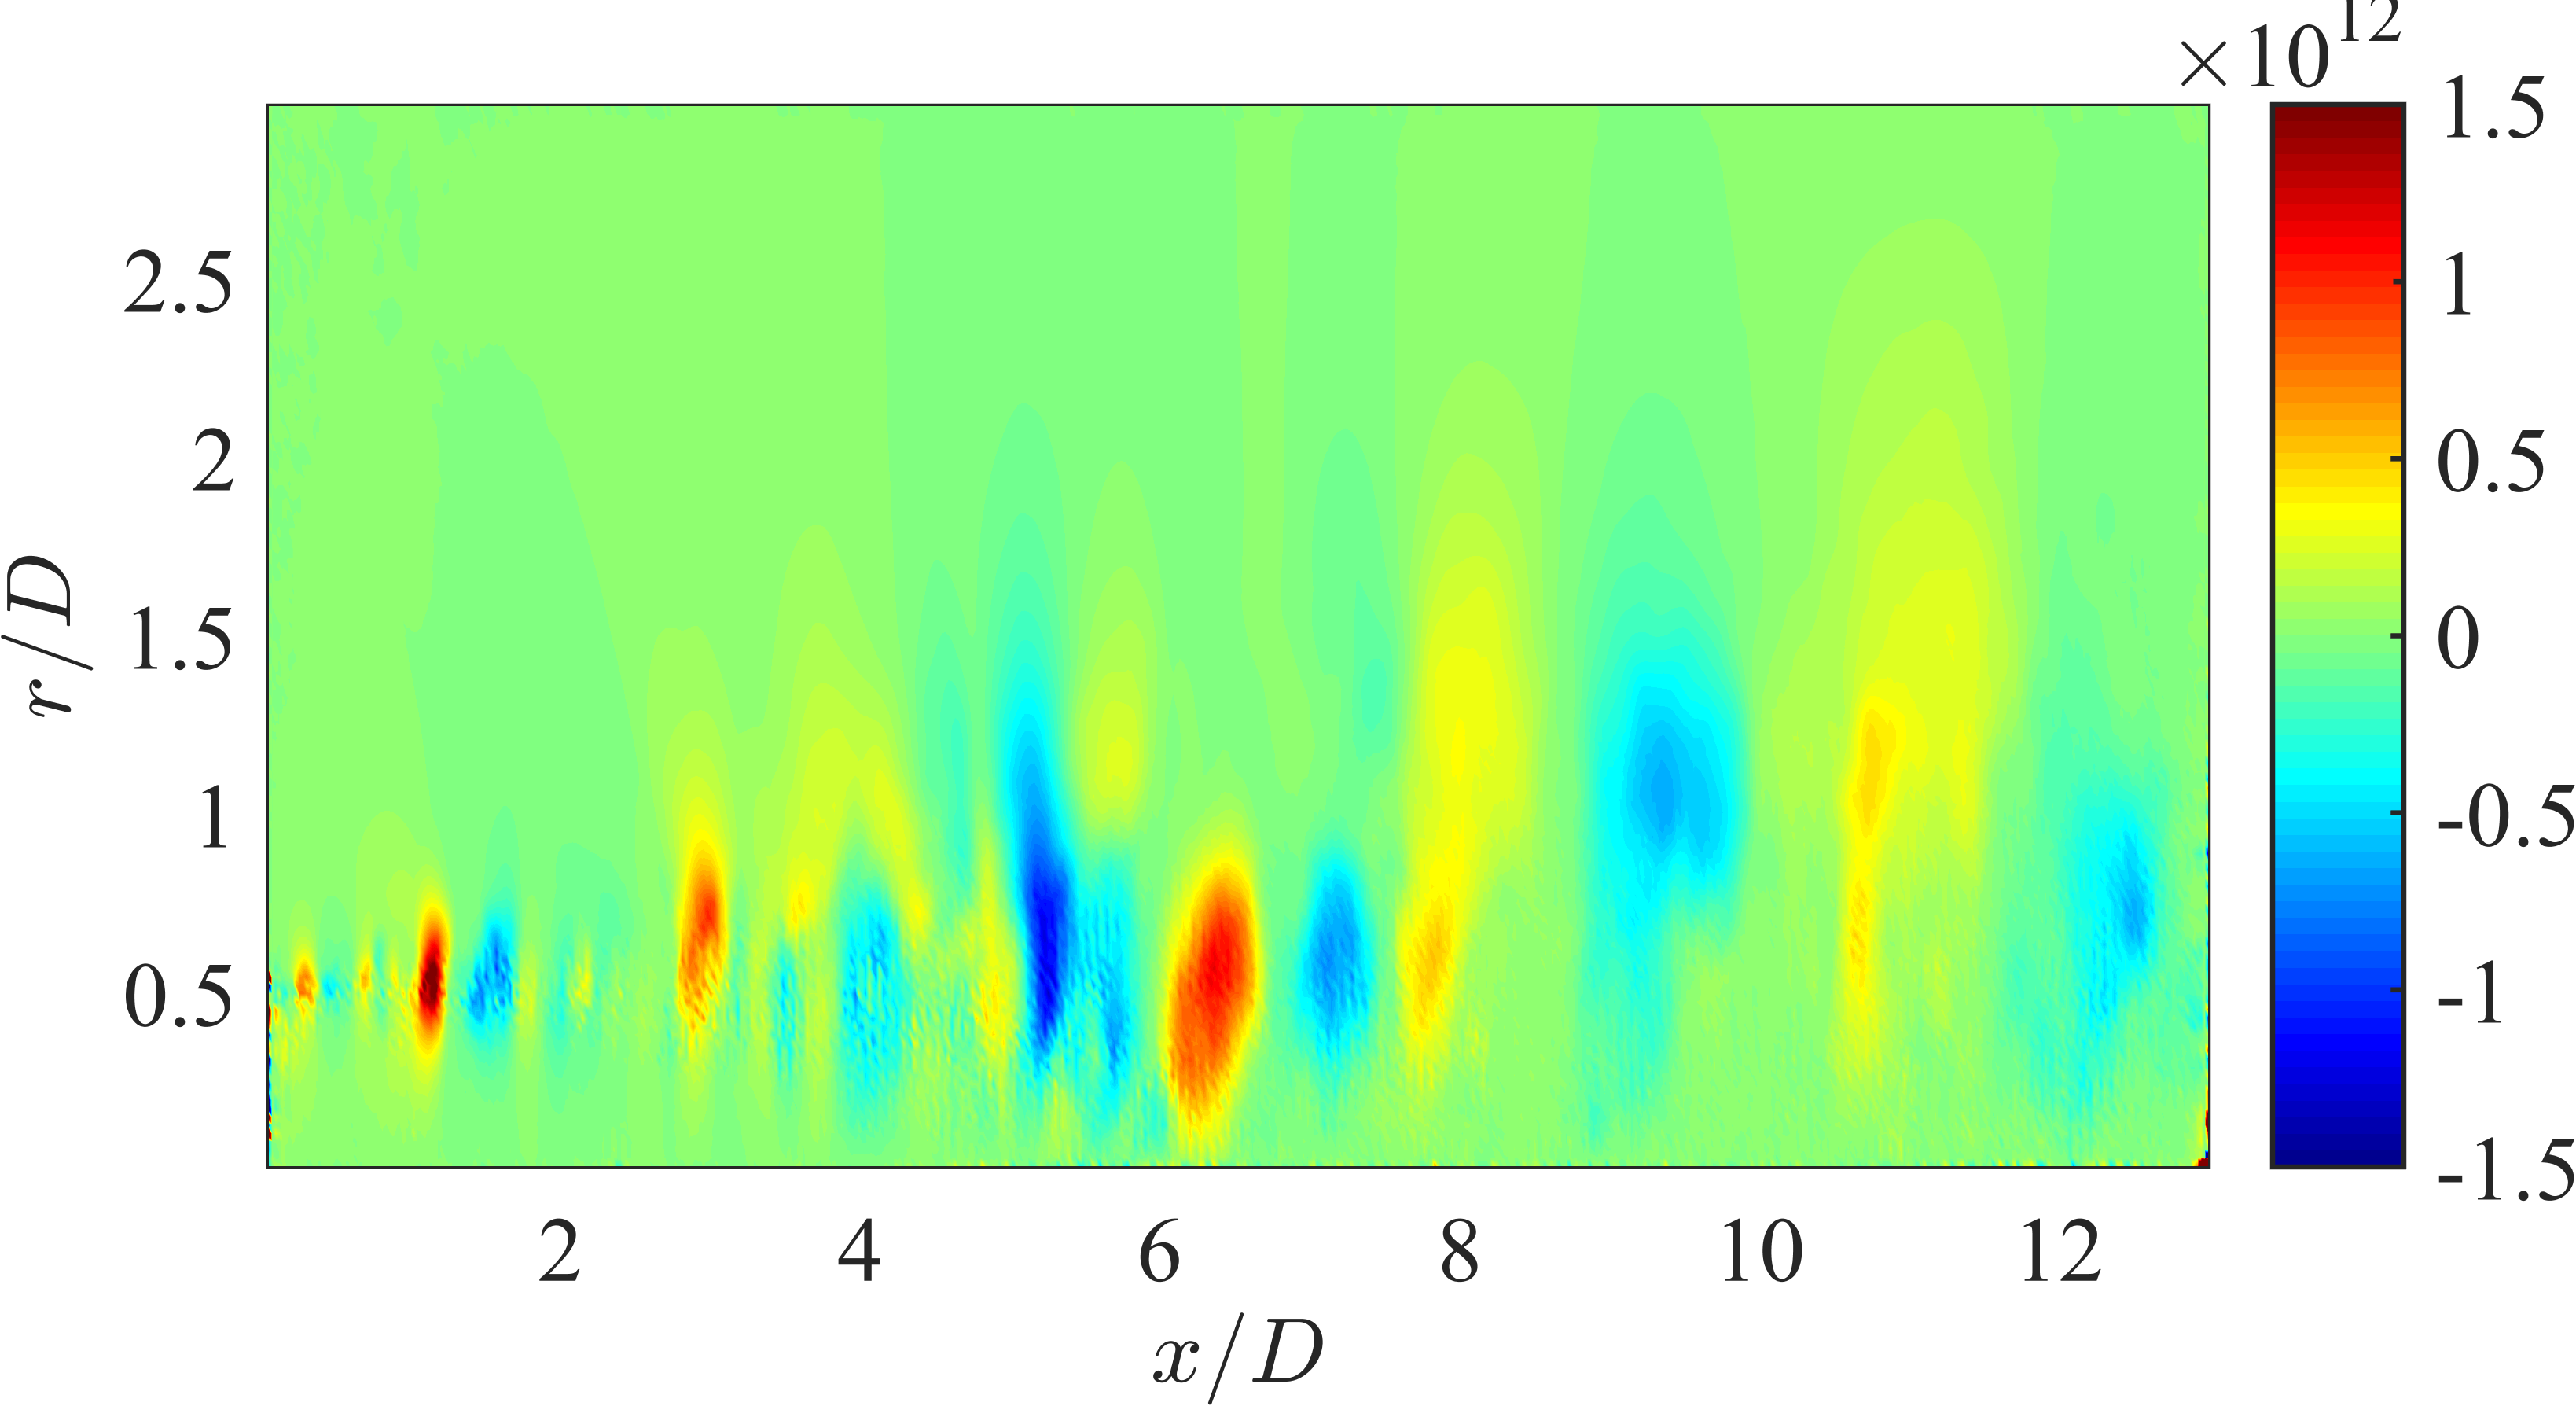
\includegraphics[width = 3.5in]{Figures/ch5_valid_Inst_source.png}
	\caption{Instantaneous source field for the same conditions as \fig{fig:valid_helmholtz}.}
	\label{fig:valid_source}
\end{figure}

\subsection{Wavepackets in the Pseudo-Pressure Field}
The signature of the large-scale structures in the irrotational near-field pressure has been well-known for some time.
As discussed in \sect{sect:nearfield}, the near-field pressure response to a large-scale structure takes the form of a compact wave which is modulated in amplitude and spatial extent as it convects through the jet shear layer; the near-field response to excitation-induced large-scale structures is discussed in more detail by \citet{Sinha2012}.
Similar results have also been found by \citet{Tinney2008} in a natural, subsonic jet.
Per Ribner's analysis, these near-field pressure signatures are related to the noise sources and hence can serve as a useful validation of the computed pseudo-pressure fields since they are close physical analogues (though the hydrodynamic component of the irrotational near-field pressure isn't strictly incompressible, compressibility effects are minor). 
\begin{figure}
	\centering
%	\begin{subfigure}{.5\textwidth}
%		\centering
		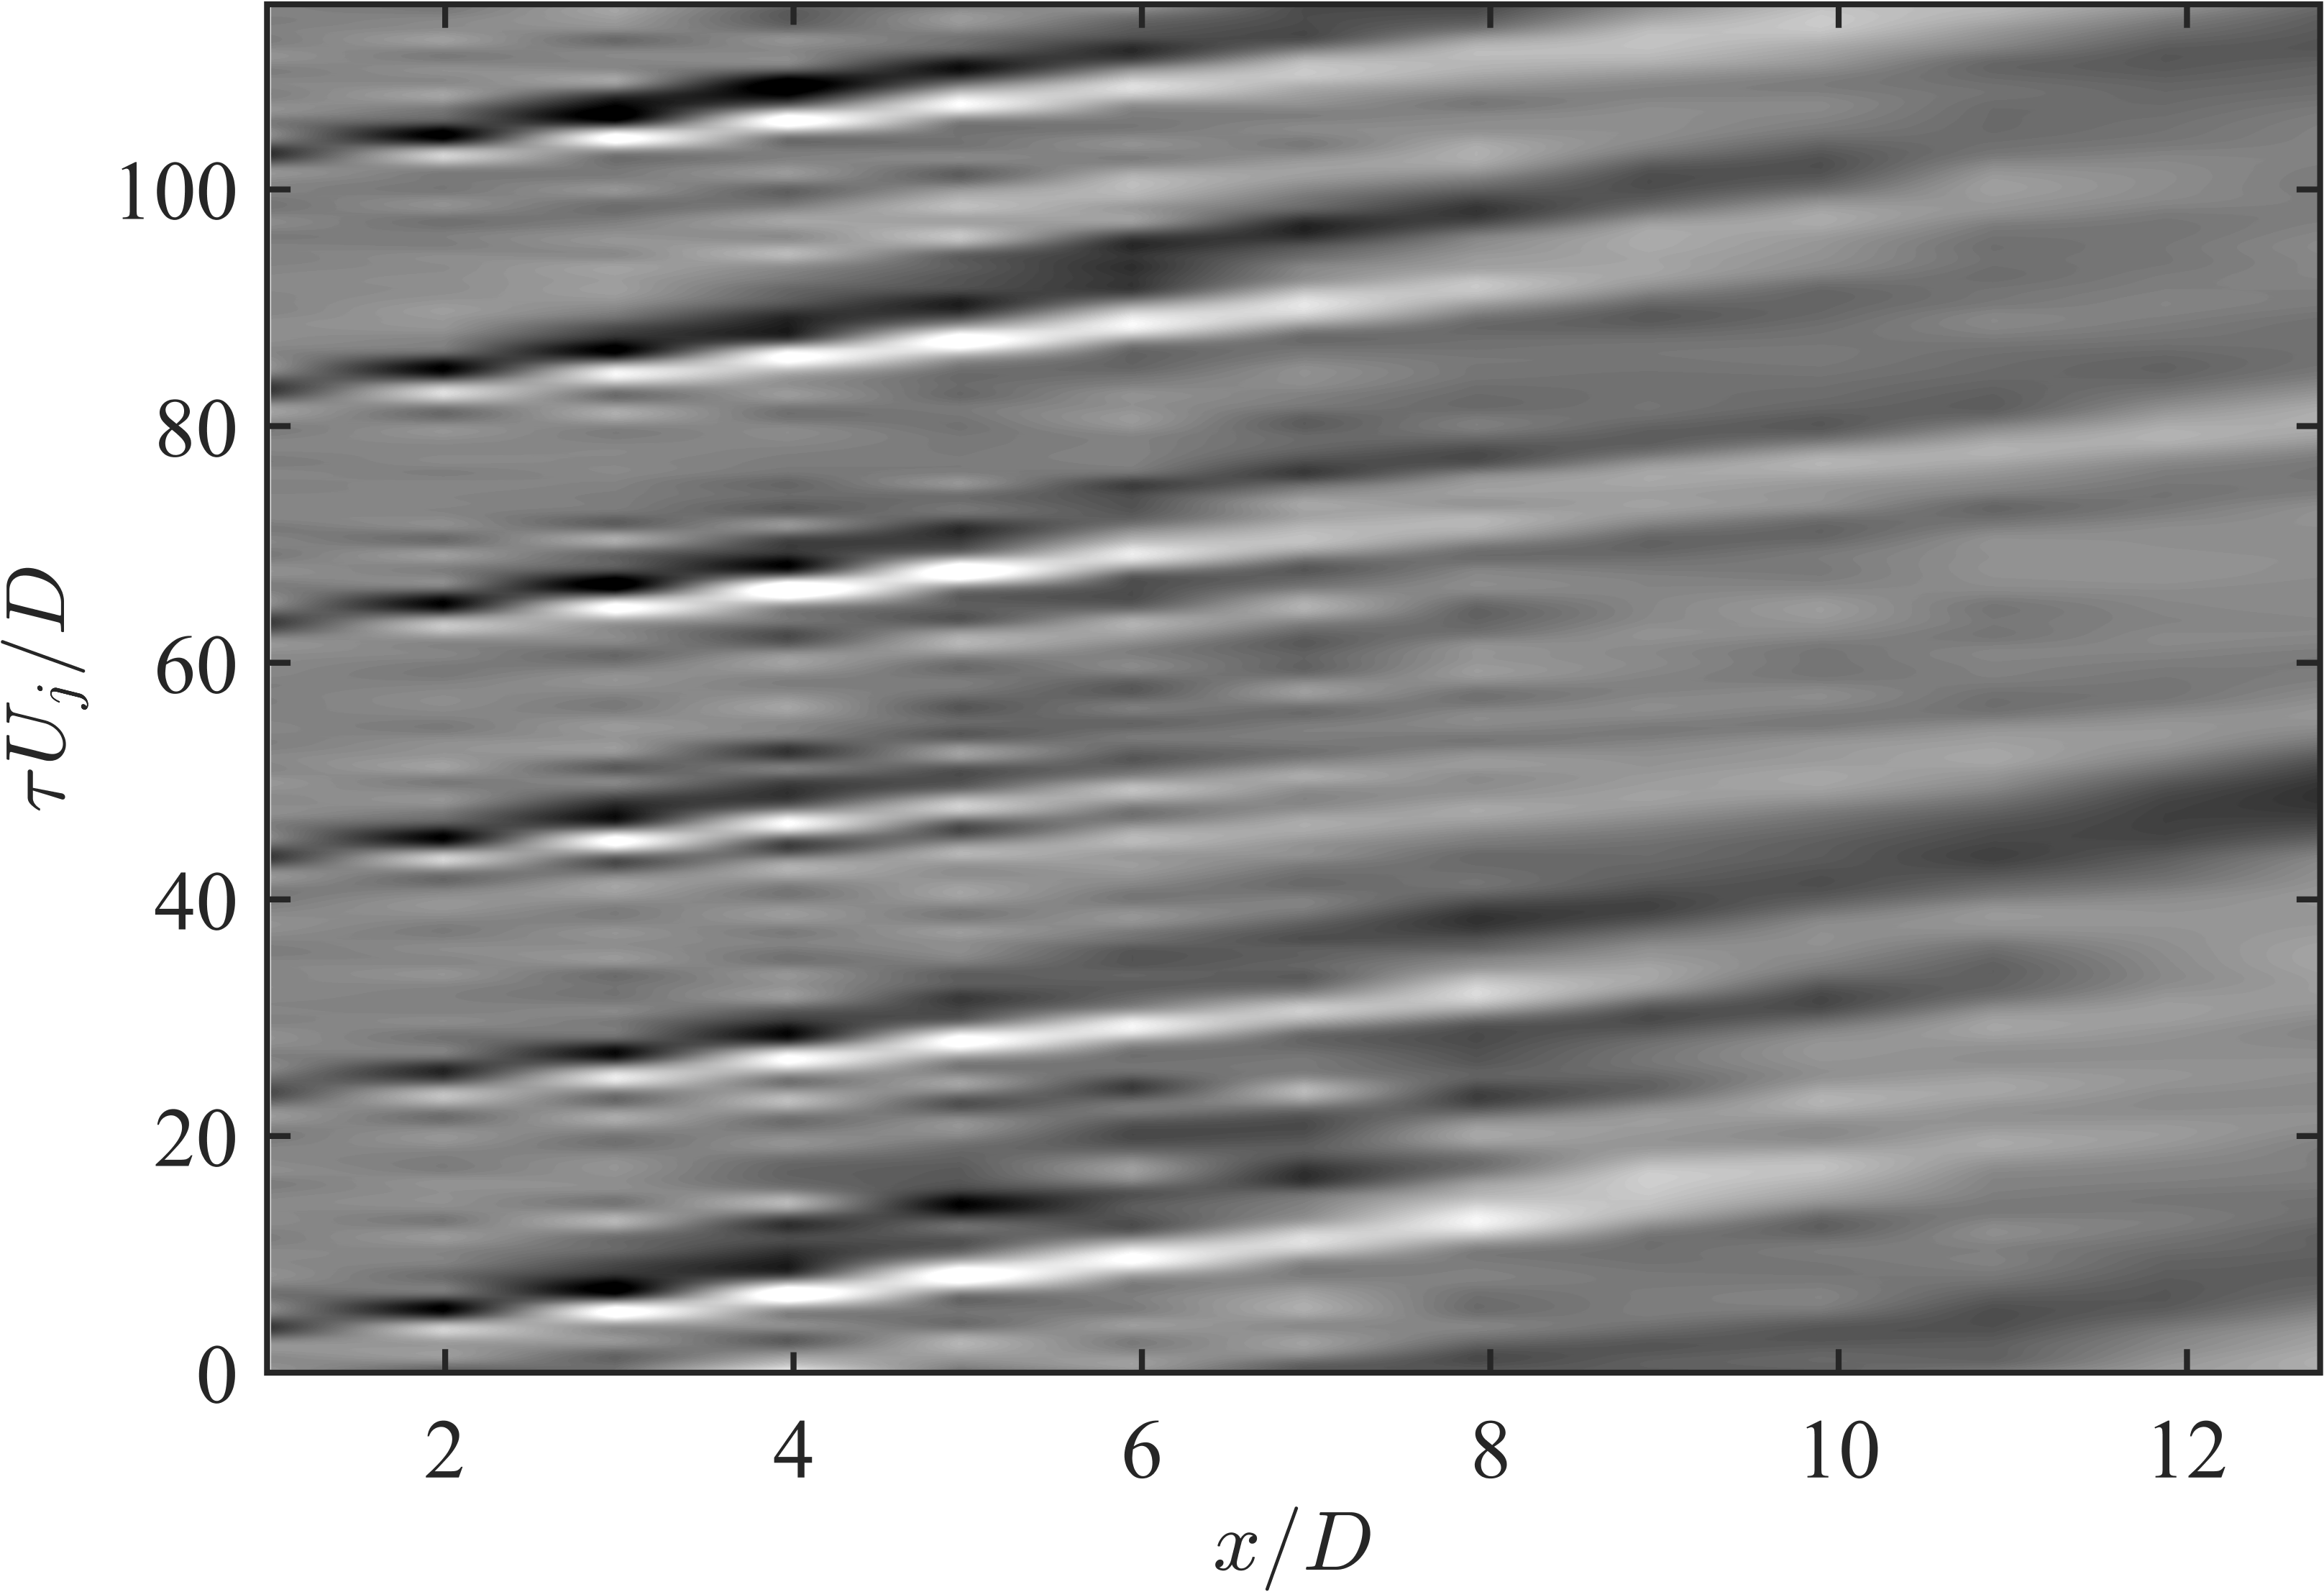
\includegraphics[width=0.45\linewidth]{Figures/ch5_st005_NearField_wvpkts.png}
%		\caption{}
%	\end{subfigure}%
%	\begin{subfigure}{.5\textwidth}
%		\centering
		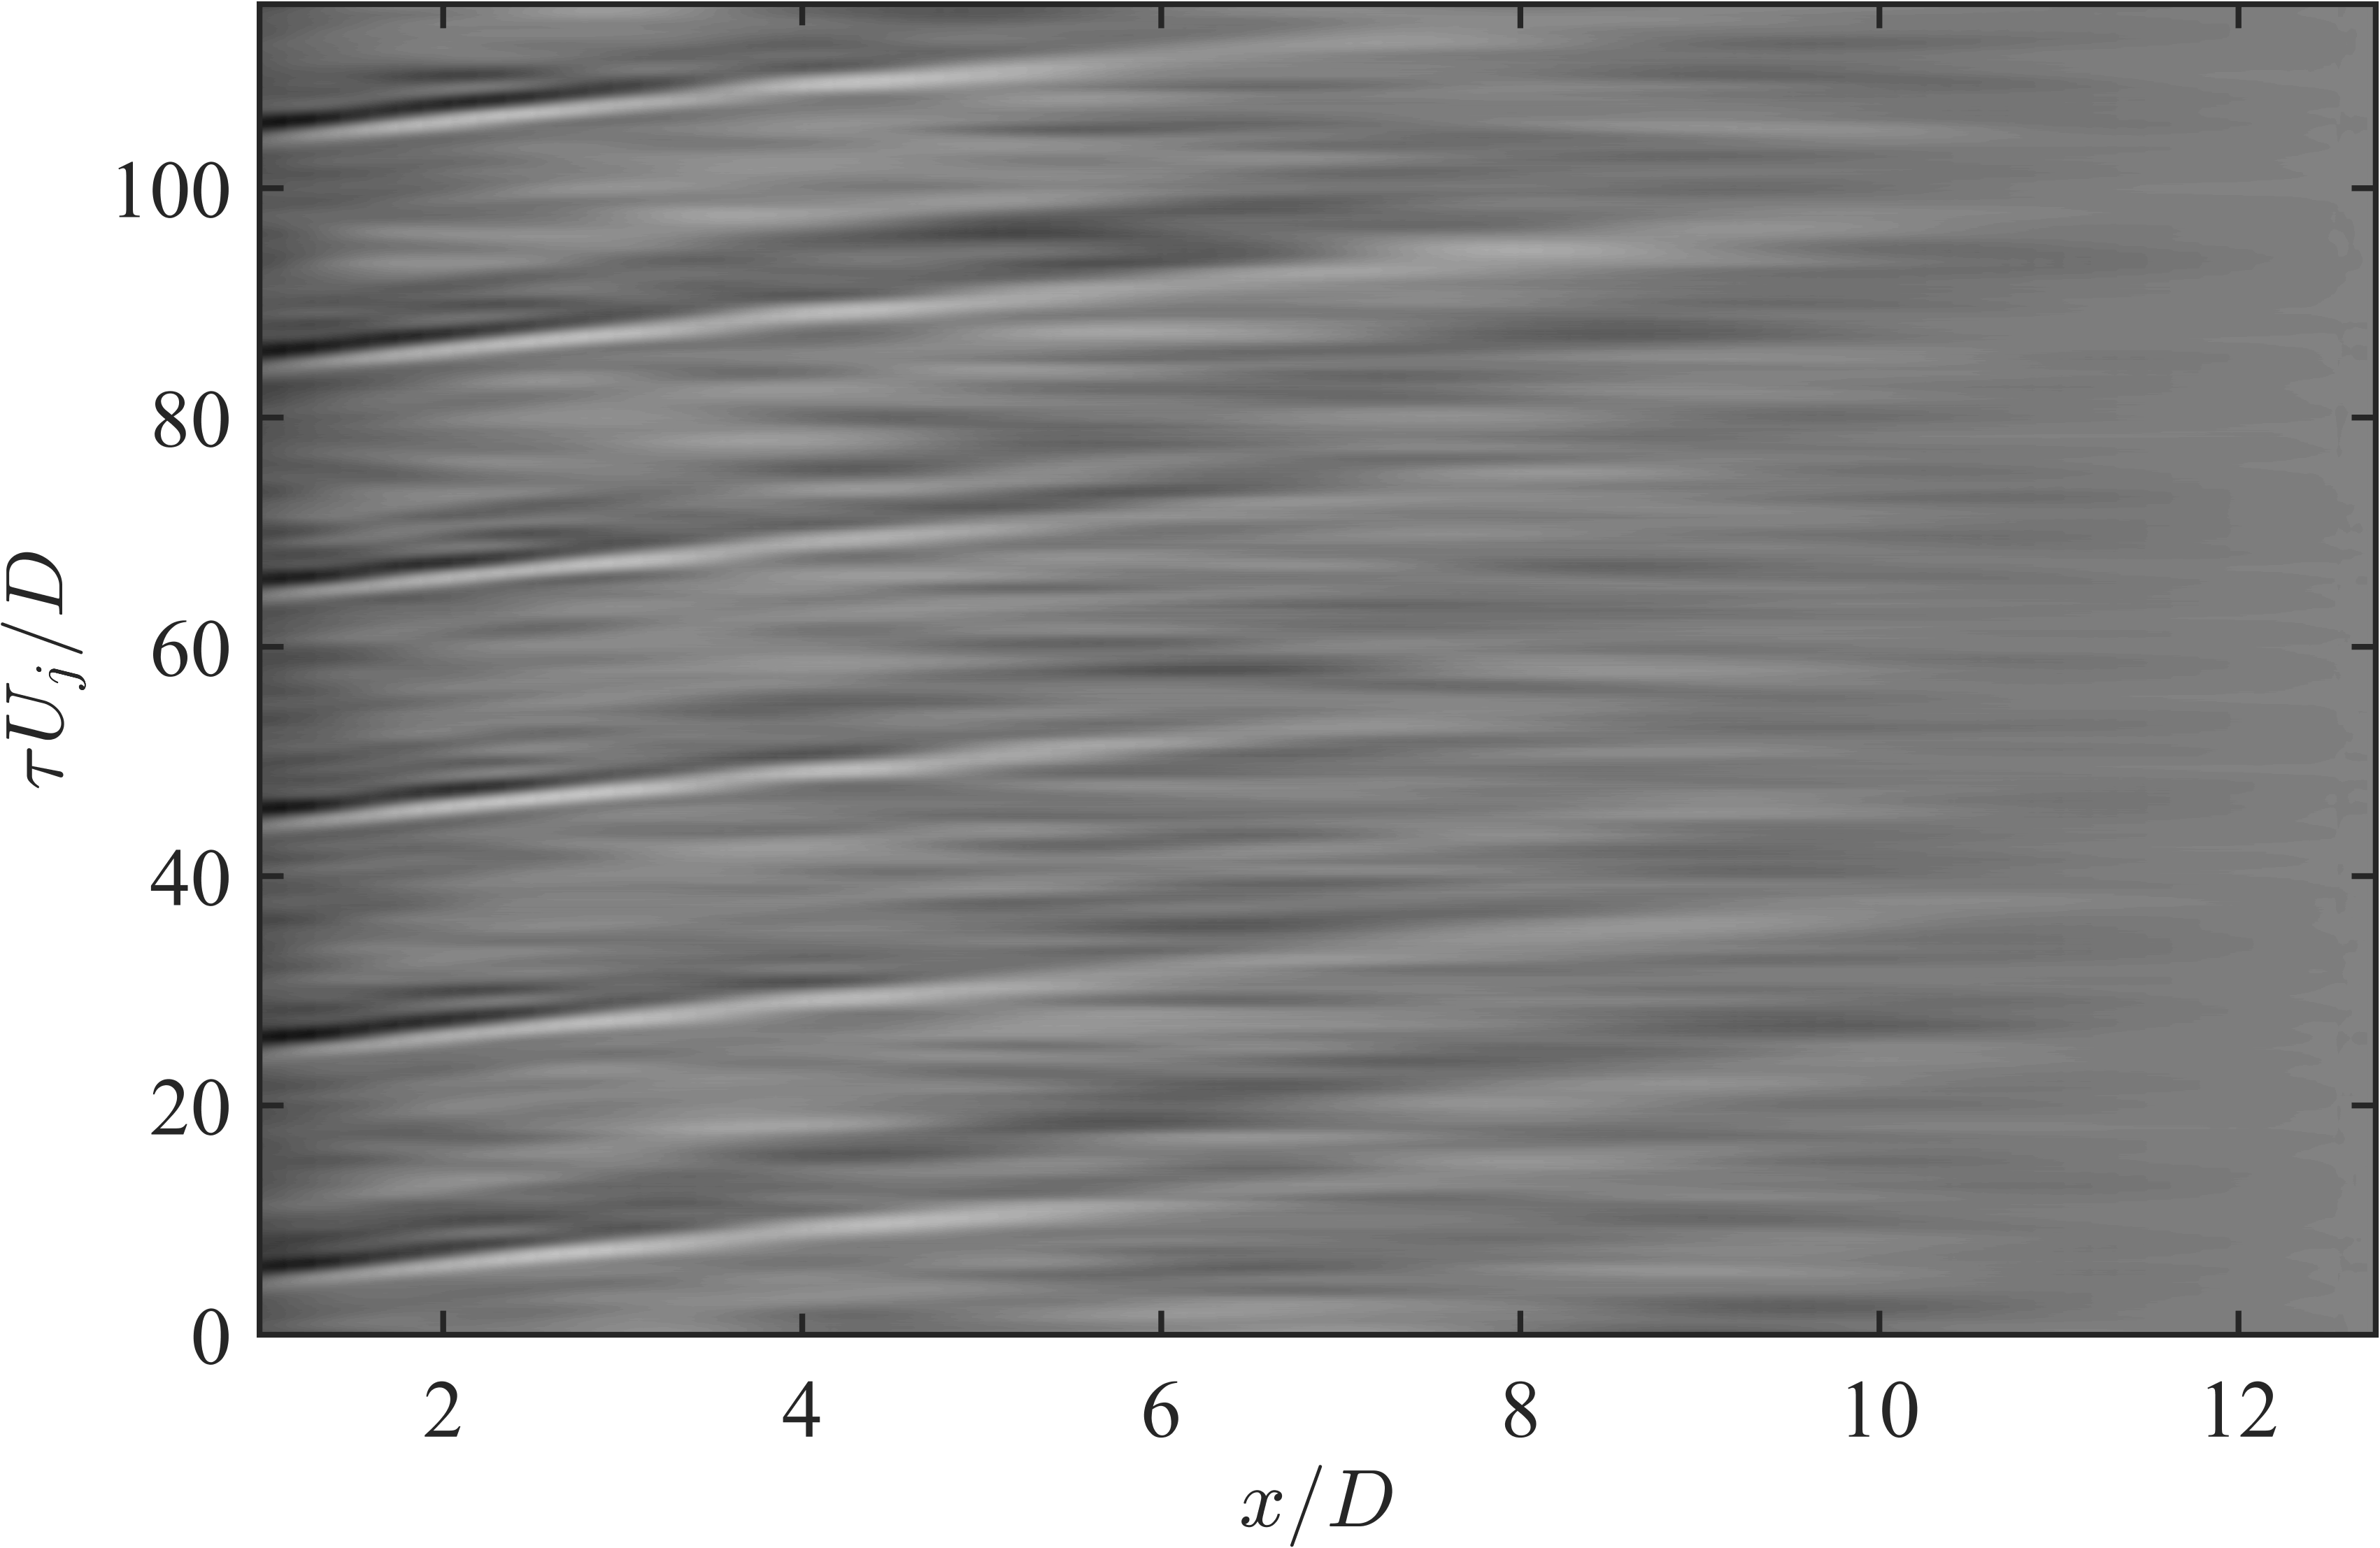
\includegraphics[width=0.45\linewidth]{Figures/ch5_st005_FlowField_wvpkts.png}\\
%		\caption{}
%	\end{subfigure}\\
%	\begin{subfigure}{.5\textwidth}
%		\centering
		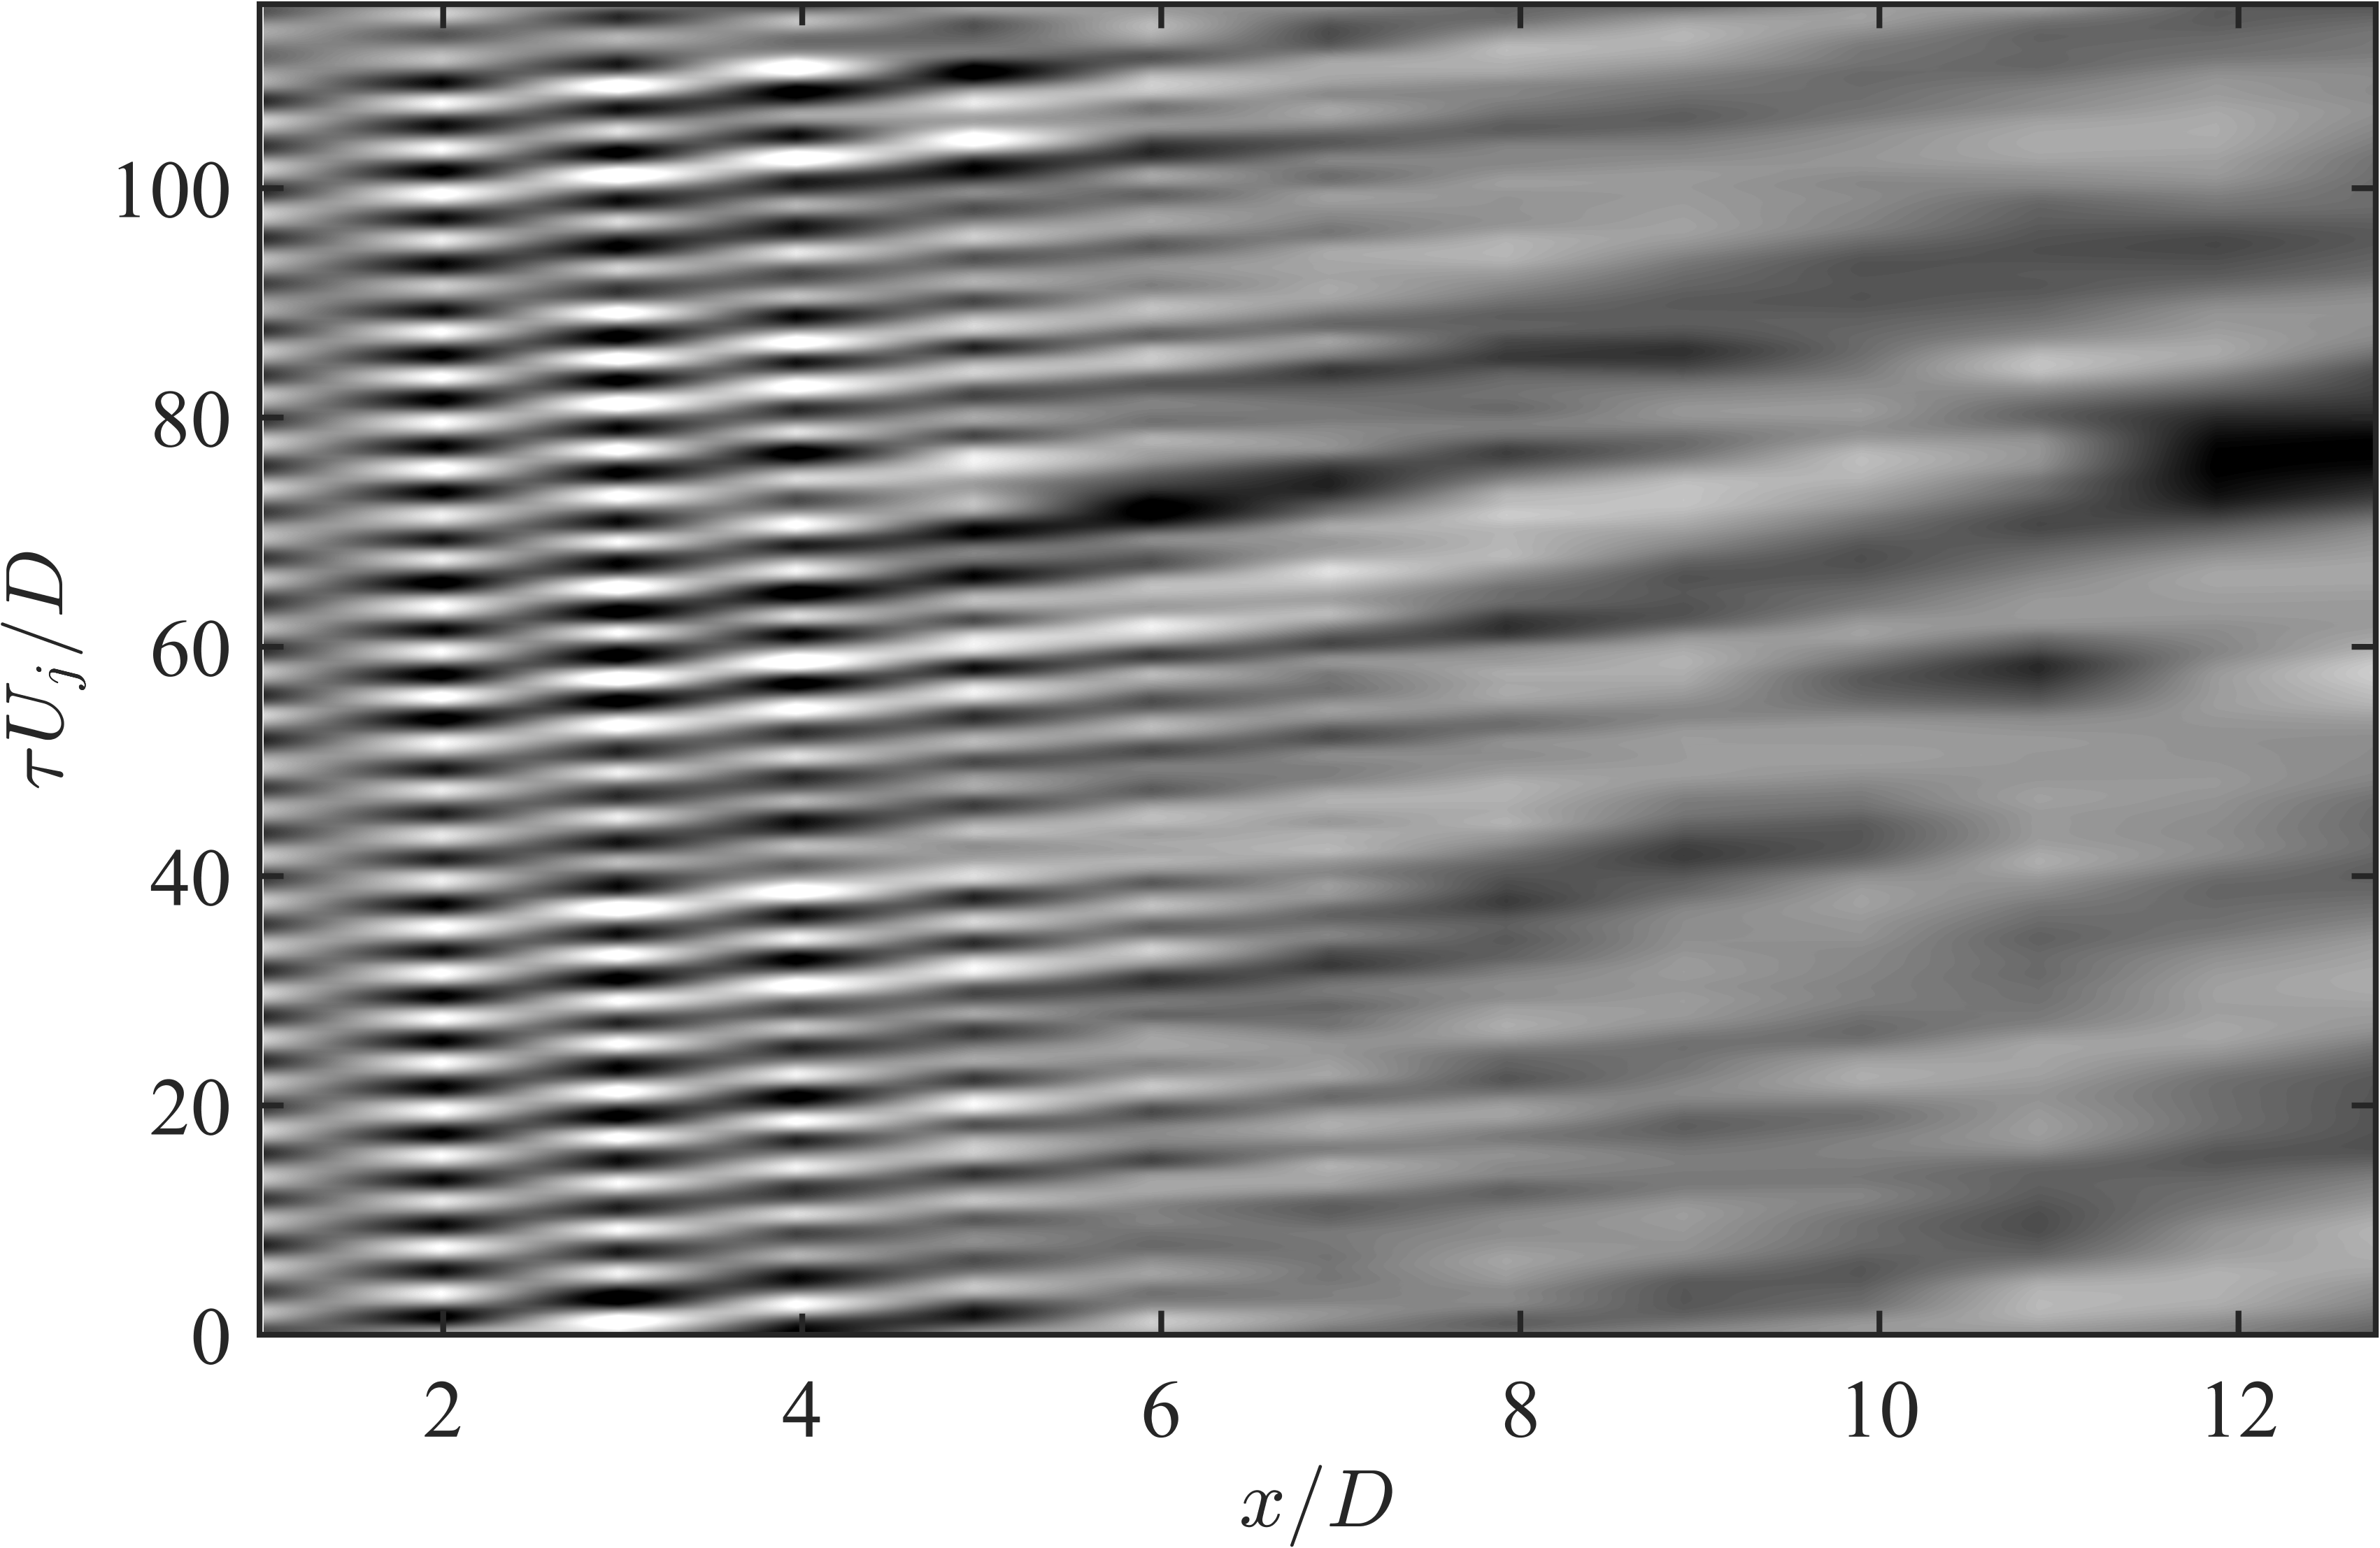
\includegraphics[width=0.45\linewidth]{Figures/ch5_st025_NearField_wvpkts.png}
%		\caption{}
%	\end{subfigure}%
%	\begin{subfigure}{.5\textwidth}
%		\centering
		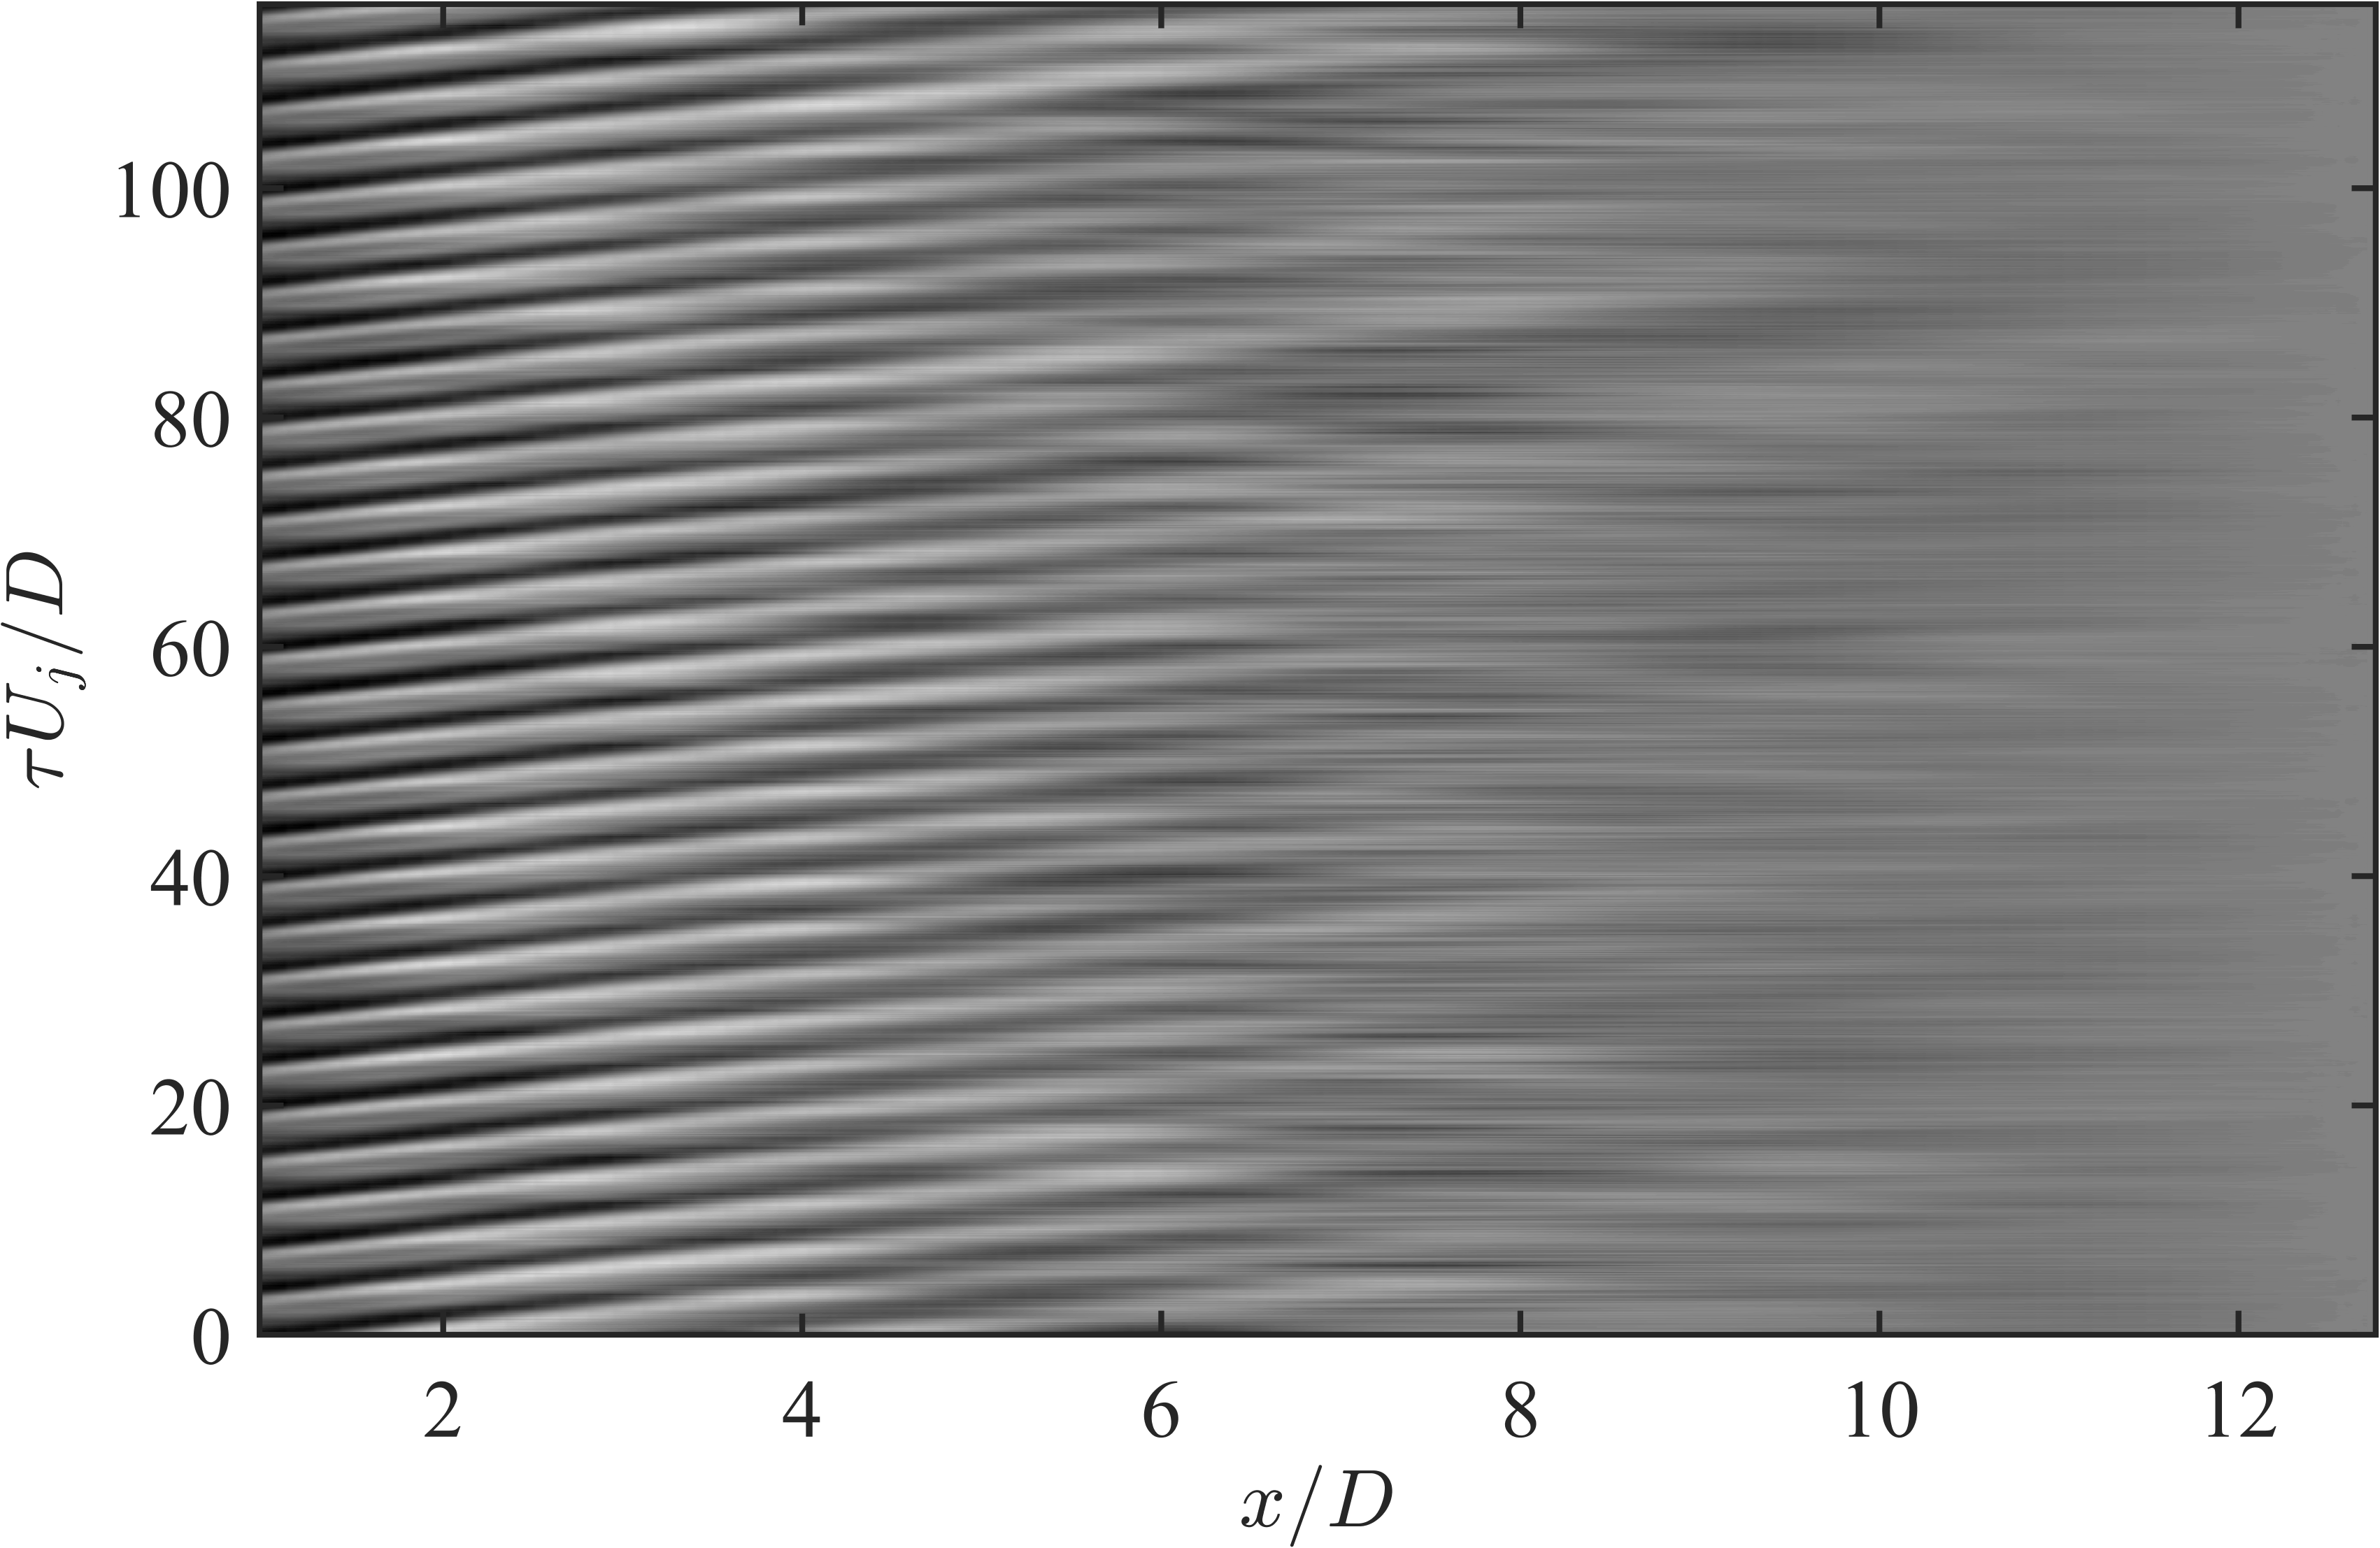
\includegraphics[width=0.45\linewidth]{Figures/ch5_st025_FlowField_wvpkts.png}
%		\caption{}
%	\end{subfigure}
	\caption{Comparison of wavepackets measured from the hydrodynamic component of the irrotational near-field (a,c) against those in the computed pseudo-pressure field (b,d) for $St_{DF} = 0.05$ (a,b) and $St_{DF} = 0.25$ (c,d). A constant intensity map of $\pm 500$ Pa was used for all plots, and the experimentally measured near-field pressure was acquired \textbf{separately} from the velocity fields used to compute the pseudo-pressure.}
	\label{fig:flowfield_wvpkts}
\end{figure}

In \fig{fig:flowfield_wvpkts} the hydrodynamic component of the irrotational near-field pressure as measured directly by the linear microphone array is compared against the pseudo-pressure field computed from the estimated time-resolved velocity fields for two excitation frequencies. 
The `probe' locations in the pseudo-pressure field were chosen to mimic those of the near-field microphone array (just outside the shear layer and inclined $8.6^\circ$ with respect to the jet axis), just at a much higher spatial resolution.
Note that the irrotational pressure fields shown were acquired separately, i.e. near-field pressure measurements from the first experimental setup in \sect{sect:NF_methodology} are being compared against pseudo-pressure estimated using pressure measurements from the second experimental setup. 

As expected, a clear wavepacket response is observed in the pseudo-pressure fields at the excitation frequency, similar to the behavior found in the hydrodynamic near-field pressure (note that the poor spatial resolution of the near-field microphones is producing an aliasing error for $St_{DF}=0.25$).
For both fields and excitation frequencies, the wavepackets are the strongest and most coherent upstream of the end of the potential core.
Downstream of the potential core, the flow is far more disorderly, as some of the LAFPA-induced structures have broken down completely while others have not - this is most readily observed for $St_{DF}=0.05$ where more than a few LAFPA-induced structures persist weakly far downstream.
Surprisingly, the amplitude of the pseudo-pressure response is quite similar to that of the measured near-field pressure response.

The pseudo-pressure field does unfortunately exhibit a worse match against the measured near-field pressure in the far-downstream region; the cause for this is two-fold.
First, since the pressure field is highly damped with radial distance and wavenumber \citep{Arndt1997}, estimating turbulent fluctuations near the jet centerline becomes increasingly difficult as the microphones move further away due to the spreading of the shear layer; the velocity information just simply isn't present in the near-field pressure fluctuations.
Second, as the structures begin to breakdown near the end of the potential core, they lose their axisymmetry.
This presents additional difficulties for the stochastic estimation, since the near-field microphones are offset azimuthally from the PIV laser sheet a vortex captured in the streamwise slice of the flow-field is not
necessarily azimuthally-coherent and hence may not be captured by the microphones.
Given the results of \sect{sect:nearfield} as well as \citet{Hileman2005}, which found the dominant source region to be located near the end of the potential core, rather than two potential core lengths downstream, this discrepancy between the measured and computed pressure fields, though unfortunate, is not expected to effect the final results or interpretation thereof.  

\subsection{Accuracy of the Acoustic Far-field}
As will be shown in the following section, the energy of the hydrodynamic field (pseudo-pressure) is orders of magnitude greater than the acoustic field.
Hence, even slight experimental errors in the source field can overwhelm the computations for the acoustic field, rendering them next to meaningless for far-field predictions.
This problem is not unique to Ribner's or Lighthill's approaches to the acoustic analogy; it plagues vortex sound theories as well \citep{Bridges1992}.
In Ribner's dilatation acoustic analogy the source field takes the form of quadrupoles \citep{Ristorcelli1997}; the delicate interplay of these sources and sinks determining the acoustic far-field at a given spatial and temporal position.

For reference, the computed acoustic signal at a far-field observer position matching the experimental far-field array ($R = 2.57$~m from the nozzle exit, at $\phi = 30^\circ$) has been plotted against the measured signal in \fig{fig:ch5_farfield}.
For simplicity, the signals have been phase-averaged and only a single excitation period is shown.
A coherent fluctuation could conceivably be observed in the acoustic field of the impulsively-excited jet (\fig{fig:ch5_farfield}a) centered around $\tau \simeq 0.8$, however given the lack of quiet time expected in the signal this could just as easily be wishful thinking.
An offset in the time-of-arrival for the coherent wave between the calculated and measured signals could be due simply to an error in the positioning of the microphone relative to the nozzle exit, though given the poor match regardless of time-of-arrival, investigating this was deemed nonessential.
Similarly, the computed acoustic signal for the periodic excitation cases ($St_{DF} = 0.25$$ and $$0.35$) bears only vague similarities in shape and amplitude to the measured signal.
Ultimately this means of course, that the computed source field should be viewed with some level of reservation, and hence will only be analyzed in the broadest of terms.
\begin{figure}
	\centering
%	\begin{subfigure}{1\textwidth}
%		\centering
		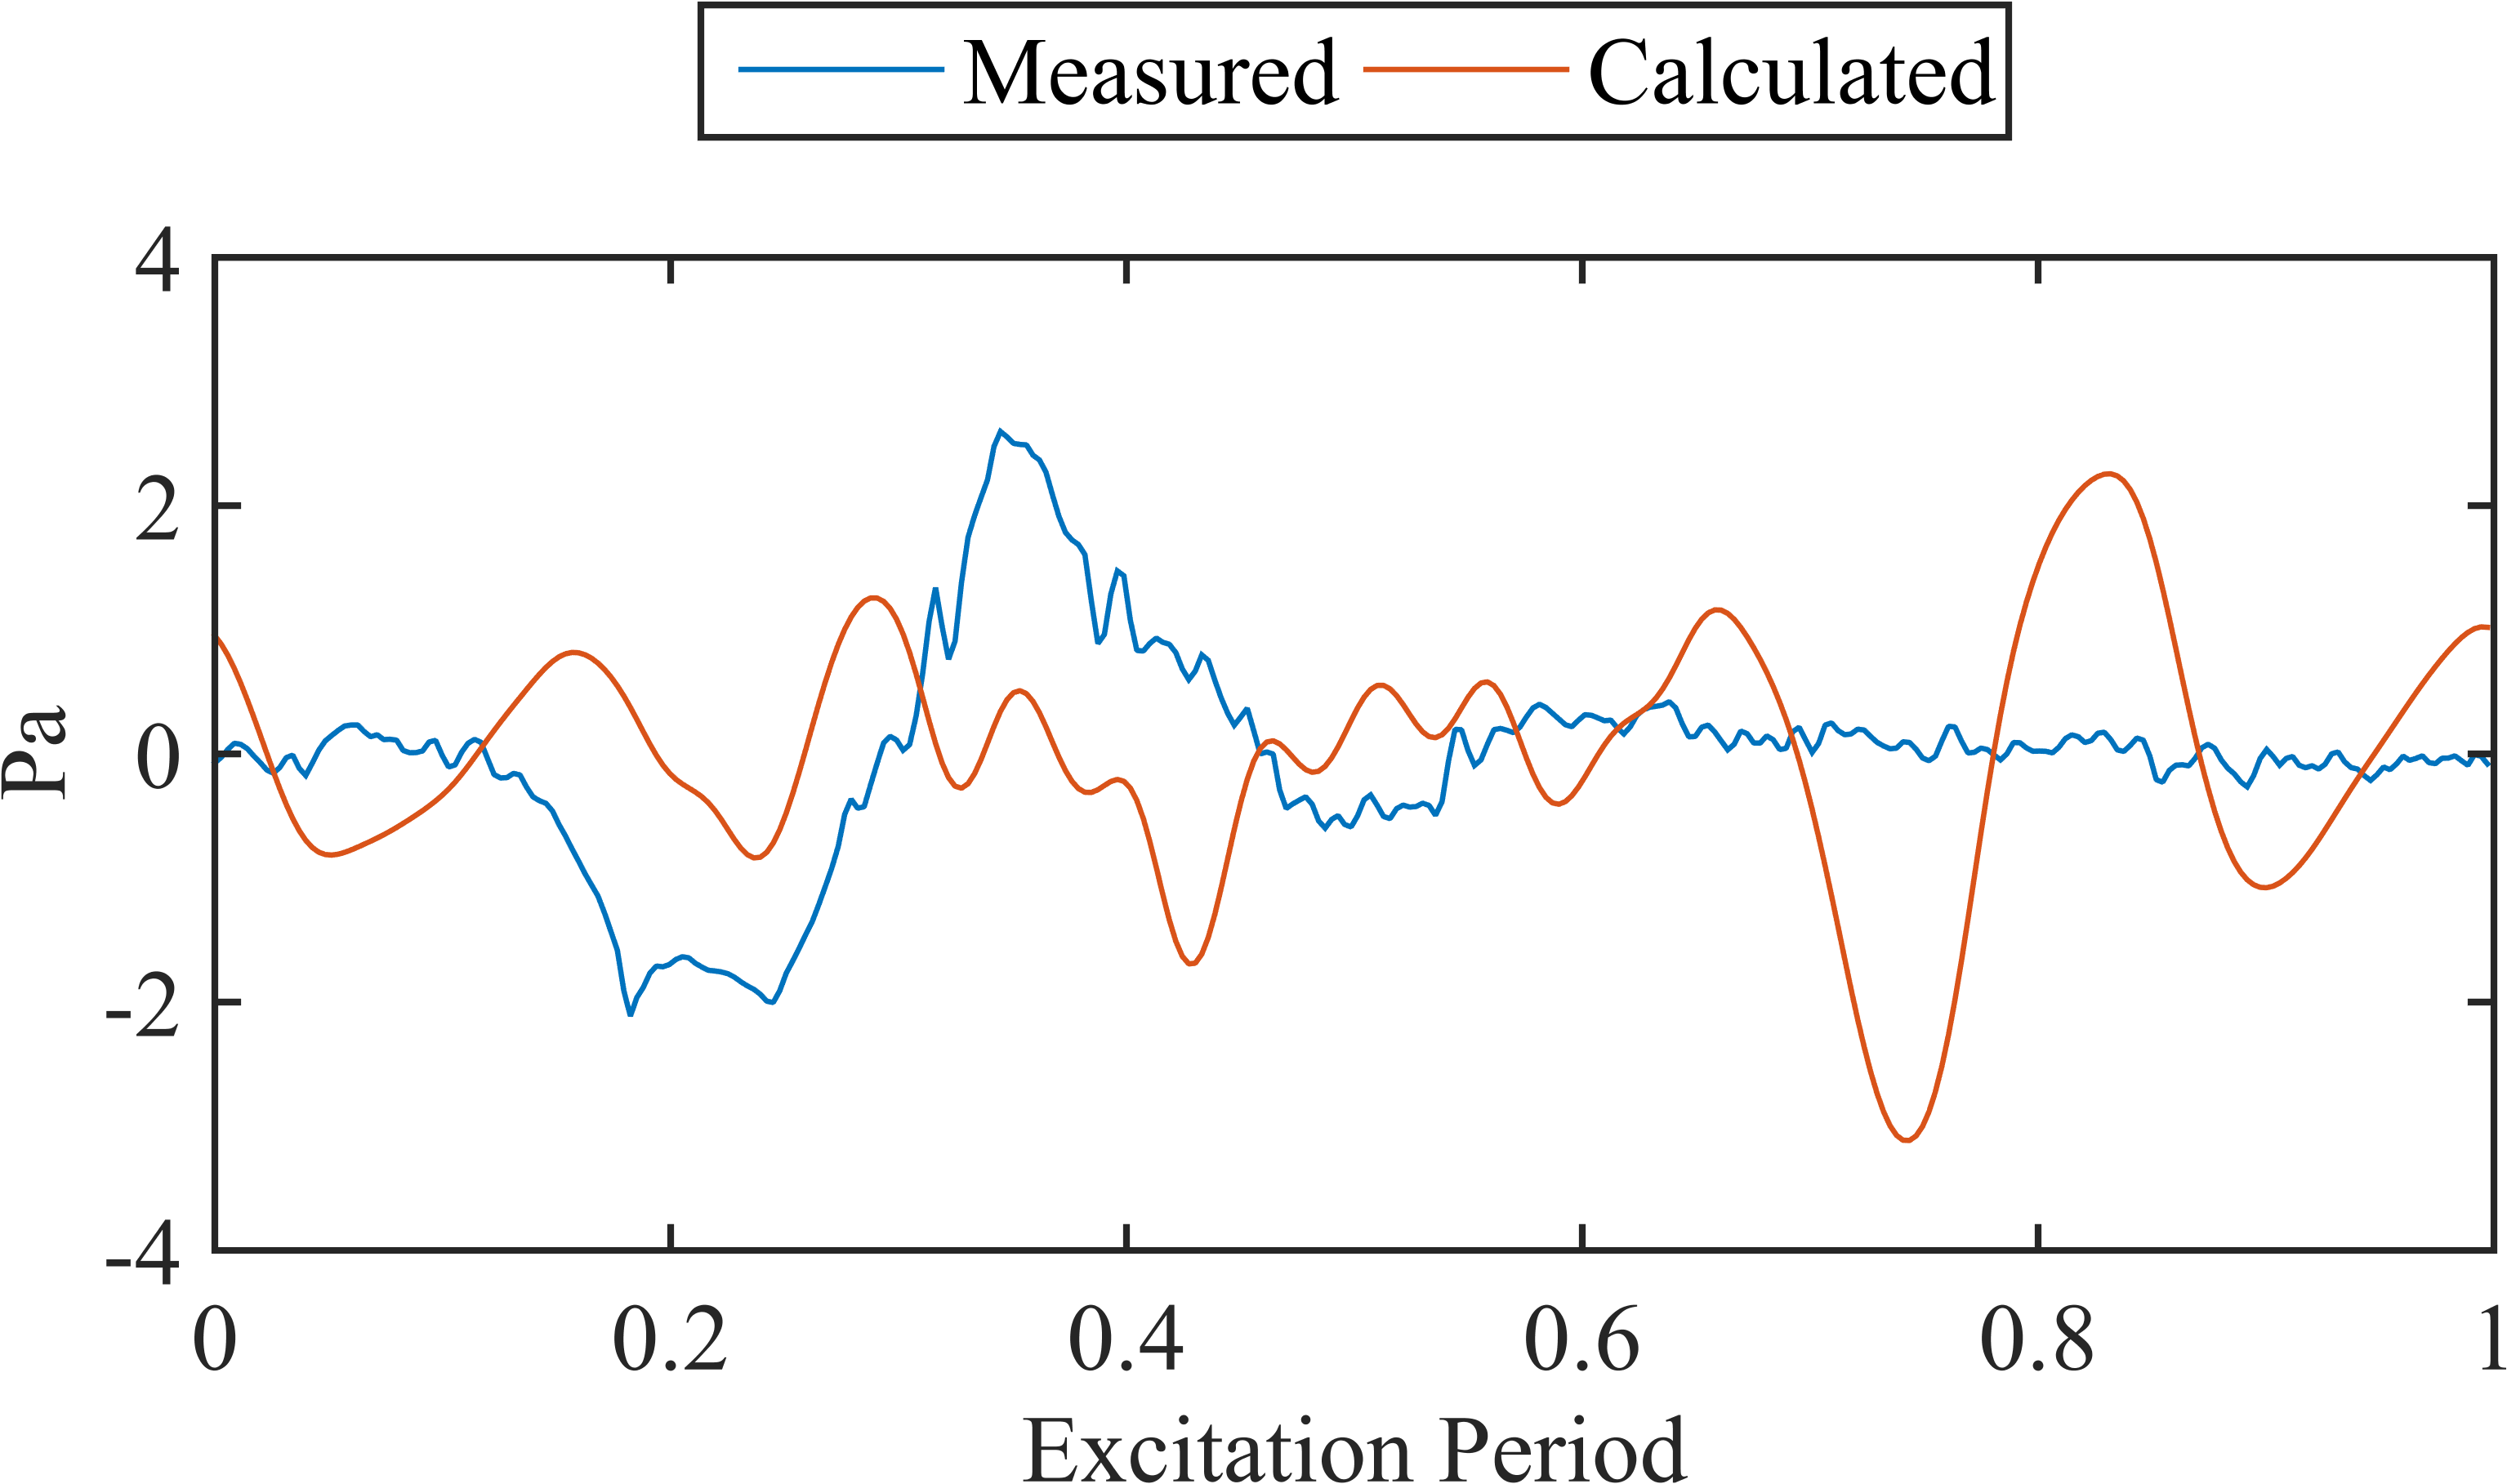
\includegraphics[width=3.5in]{Figures/ch5_St005_FF_v2.png}\\
%		\caption{$St_{DF} = 0.05$}
%		\label{fig:ch5_farfield_imp}
%	\end{subfigure}\\
%	\begin{subfigure}{1\textwidth}
%		\centering
		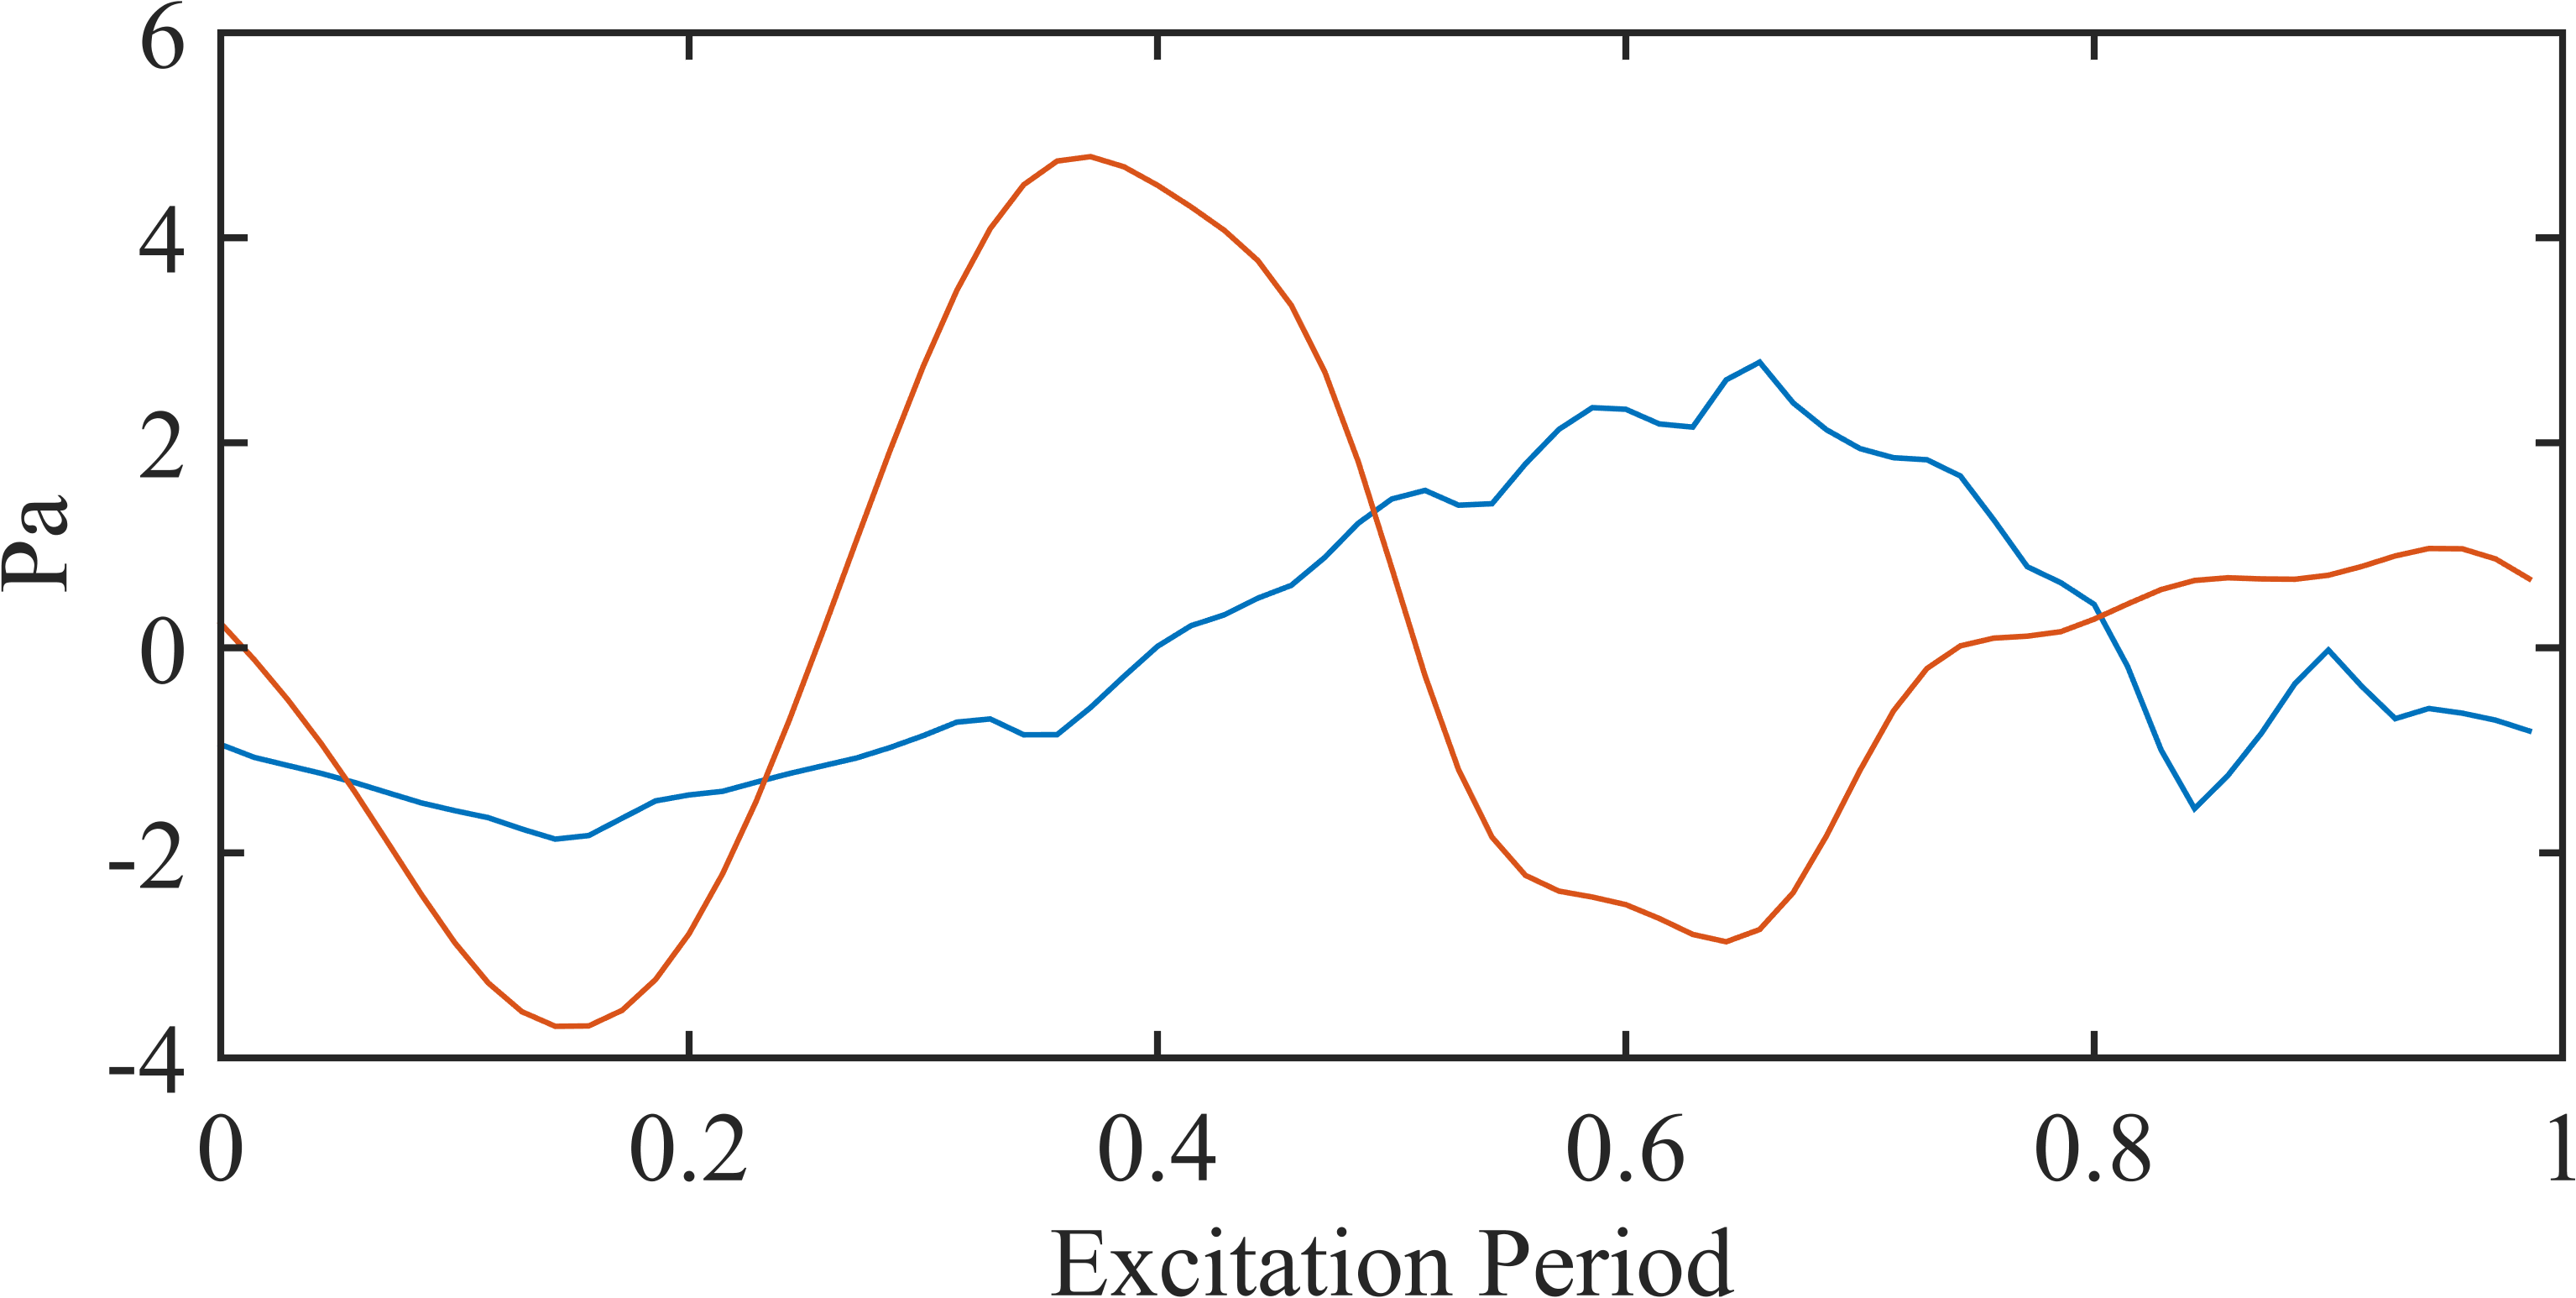
\includegraphics[width=3.5in]{Figures/ch5_St025_FF_v3.png}\\
%		\caption{$St_{DF} = 0.25$}
%	\end{subfigure}\\
%	\begin{subfigure}{1\textwidth}
%		\centering
		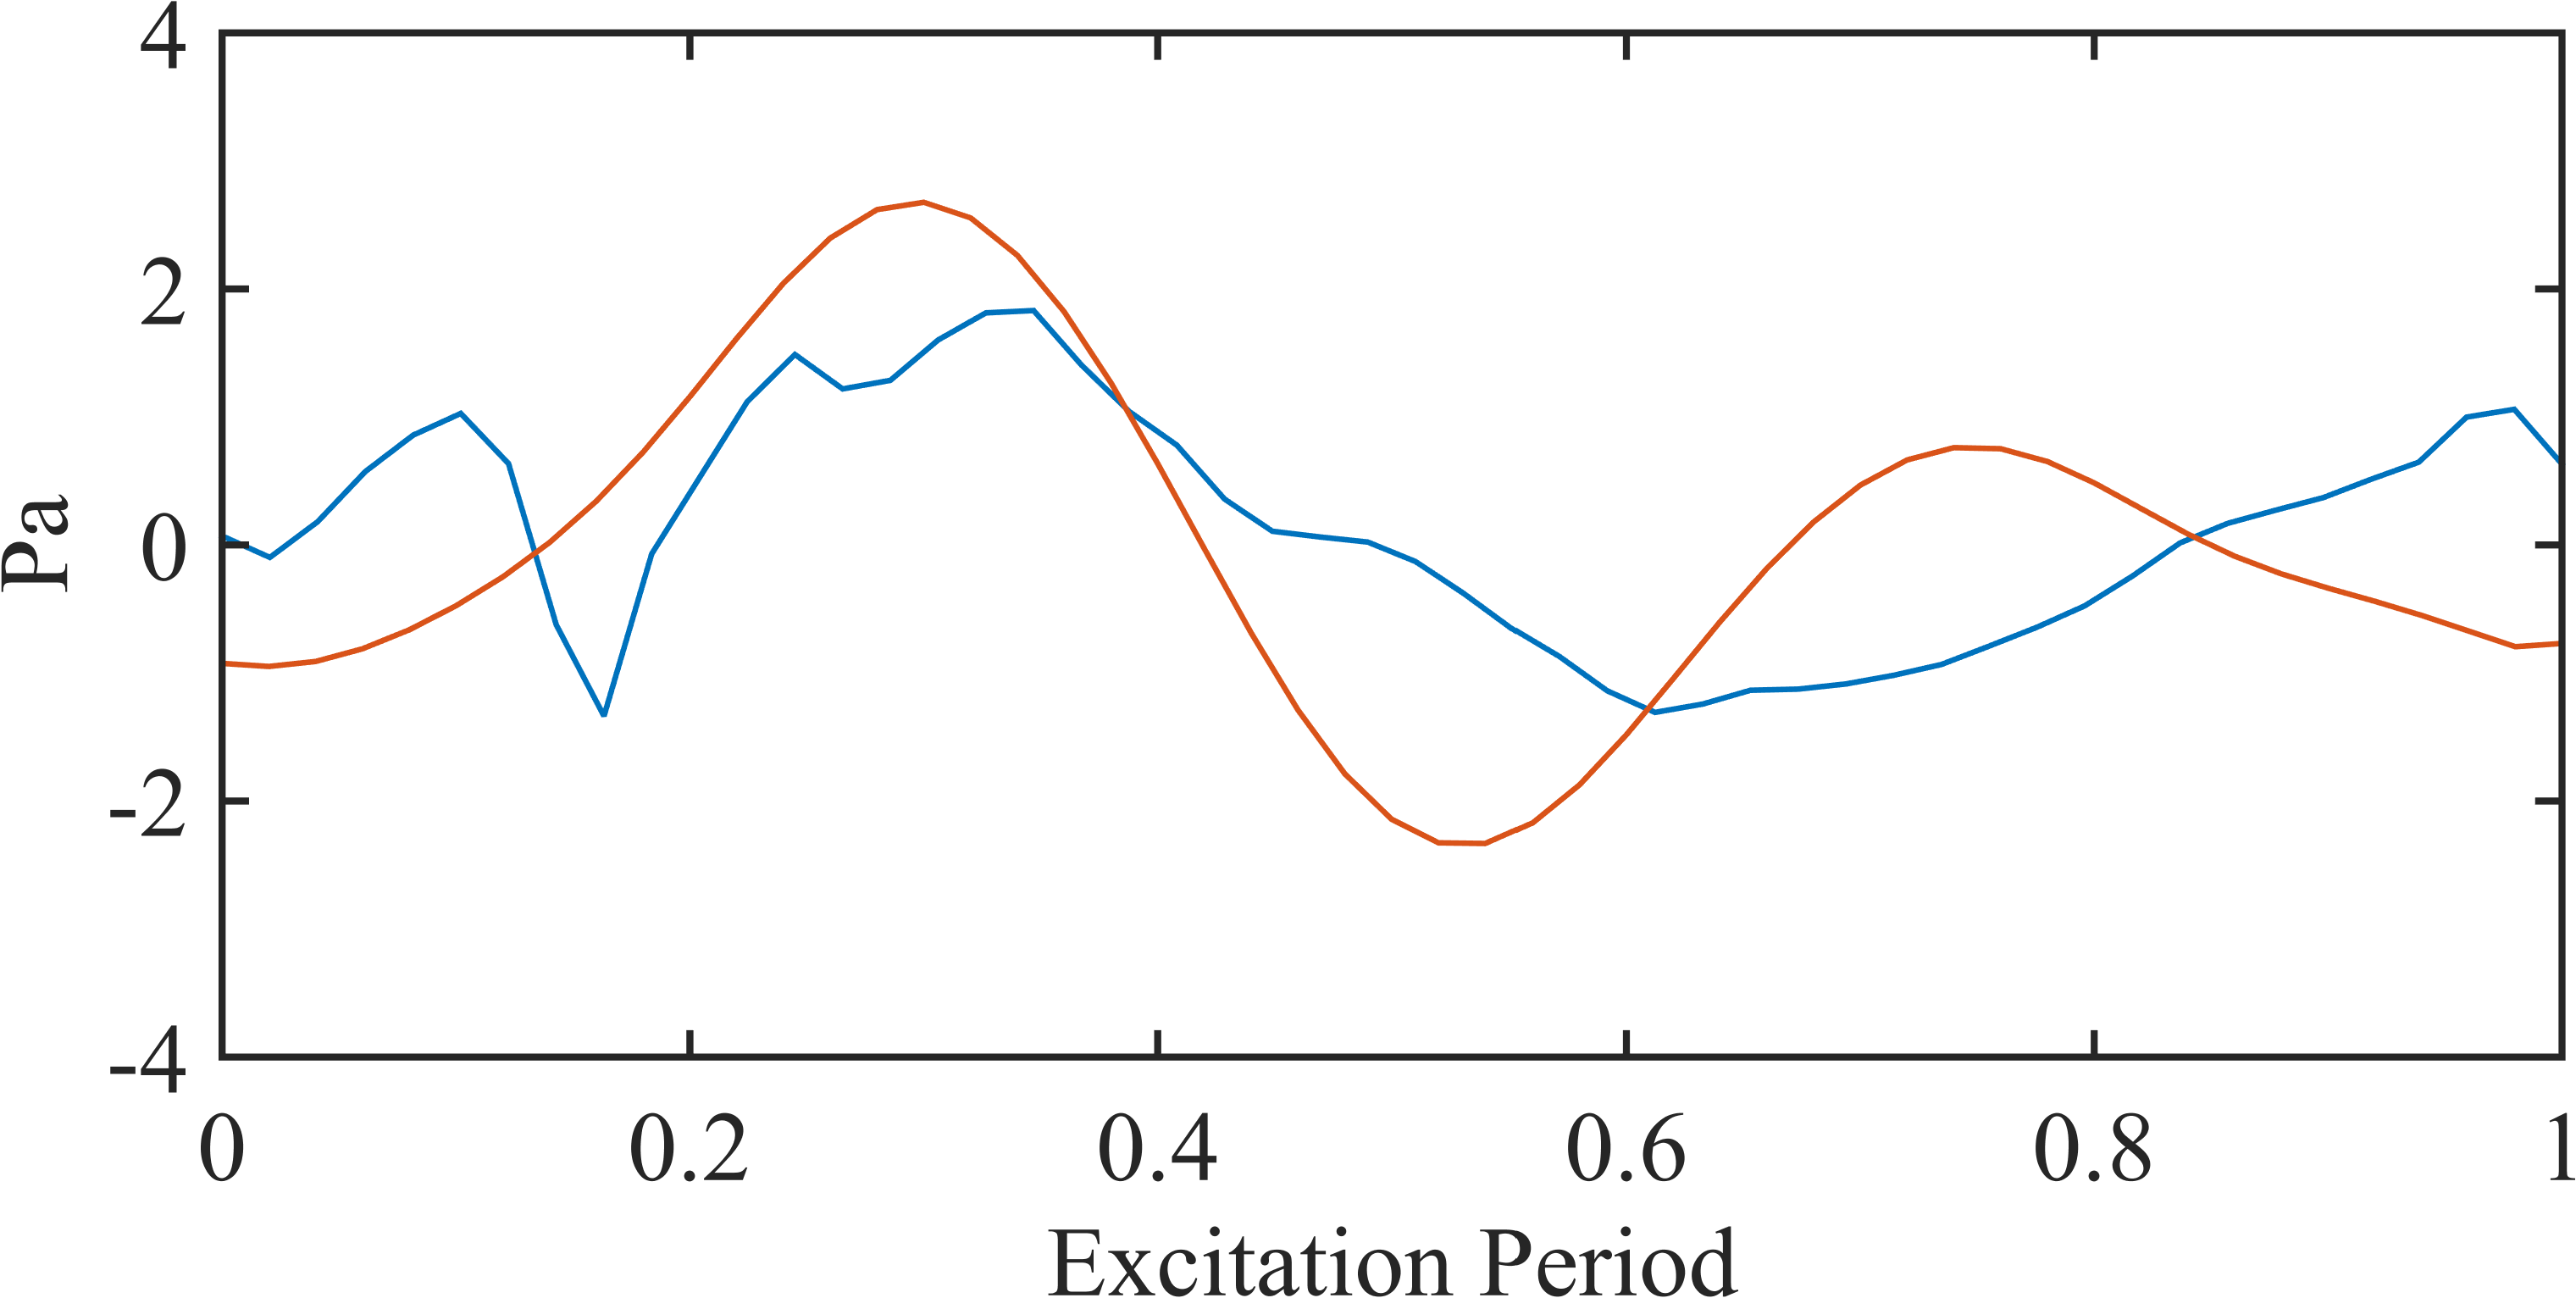
\includegraphics[width=3.5in]{Figures/ch5_St035_FF_v3.png}
%		\caption{$St_{DF} = 0.35$}
%	\end{subfigure}
	\caption{Comparison of the phase-averaged far-field signal at $30^\circ$ computed from the source field against the signal measured by the far-field microphone array.}
	\label{fig:ch5_farfield}
\end{figure}

\section{Aeroacoustic Behavior of Coherent Structures}
The pseudo-pressure field induced by the coherent vortex takes the form of a spatially-modulated traveling wave; this can be observed in \fig{fig:PSL_St005}.
A strong expansion wave is found to be centered on the vortex, preceded by an equally strong compression wave.
As the vortex convects downstream and amplifies, the radial extent of the pressure fluctuation amplifies as well; initially the pressure fluctuation is concentrated only around the jet lipline but by $x/D \simeq 2$ the pressure fluctuations reach all the way to the jet centerline.
These pressure fluctuations induce secondary, weaker fluctuations both precede and follow the dominant pair as they convect downstream.
The strength of this traveling wave is directly proportional to the strength of the vortex, as the vortices begin to break down near $x/D = 4$, the pseudo-pressure fluctuations decay rapidly as well. 
A similar behavior is observed for the periodically-excited jets ($St_{DF} = 0.25$ is shown in \fig{fig:PSL_St025}), though the pseudo-pressure field now of course takes the form of a periodic train of convecting vortices and modulating waves.
Compared to the impulse-excitation case, the radial extent of the pressure fluctuations in the periodic-excitation cases grows much more rapidly.
\begin{figure}
	\centering
%	\begin{subfigure}{0.75\textwidth}
%		\centering
		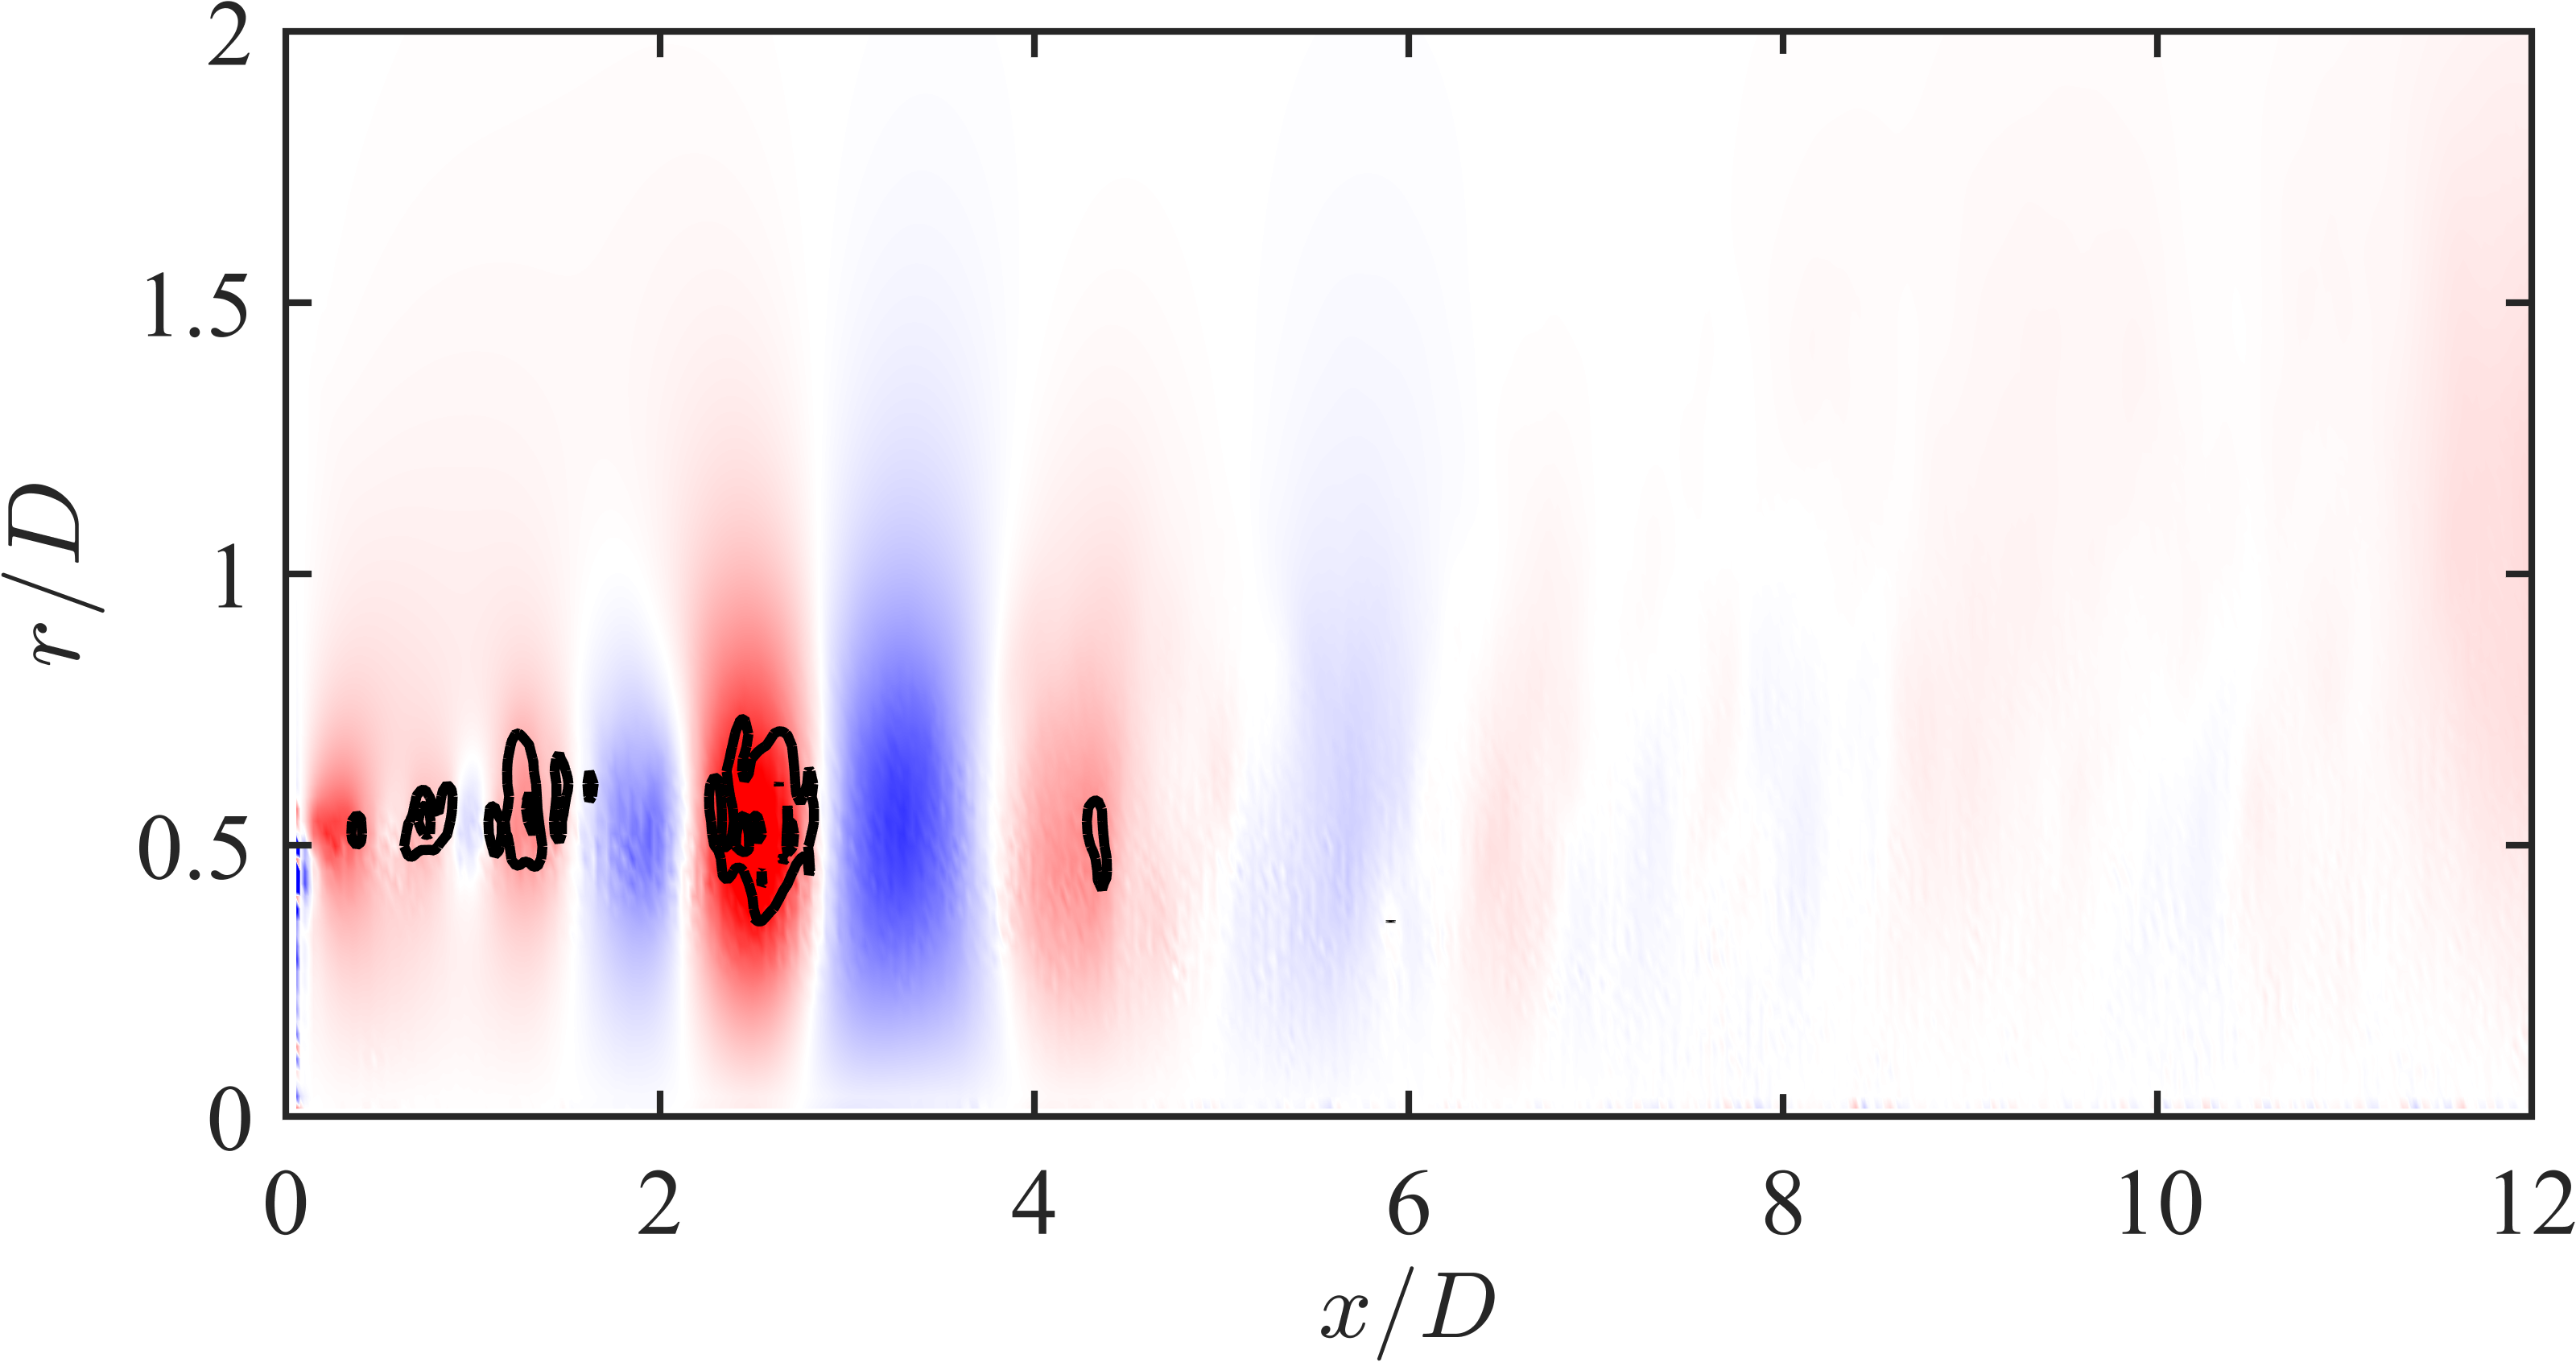
\includegraphics[width=0.65\linewidth]{Figures/ch5_St005_PSL_101.png}\\
%		\caption{$\phi = 9 \pi /16$}
%	\end{subfigure}\\
%	\begin{subfigure}{0.75\textwidth}
%		\centering
		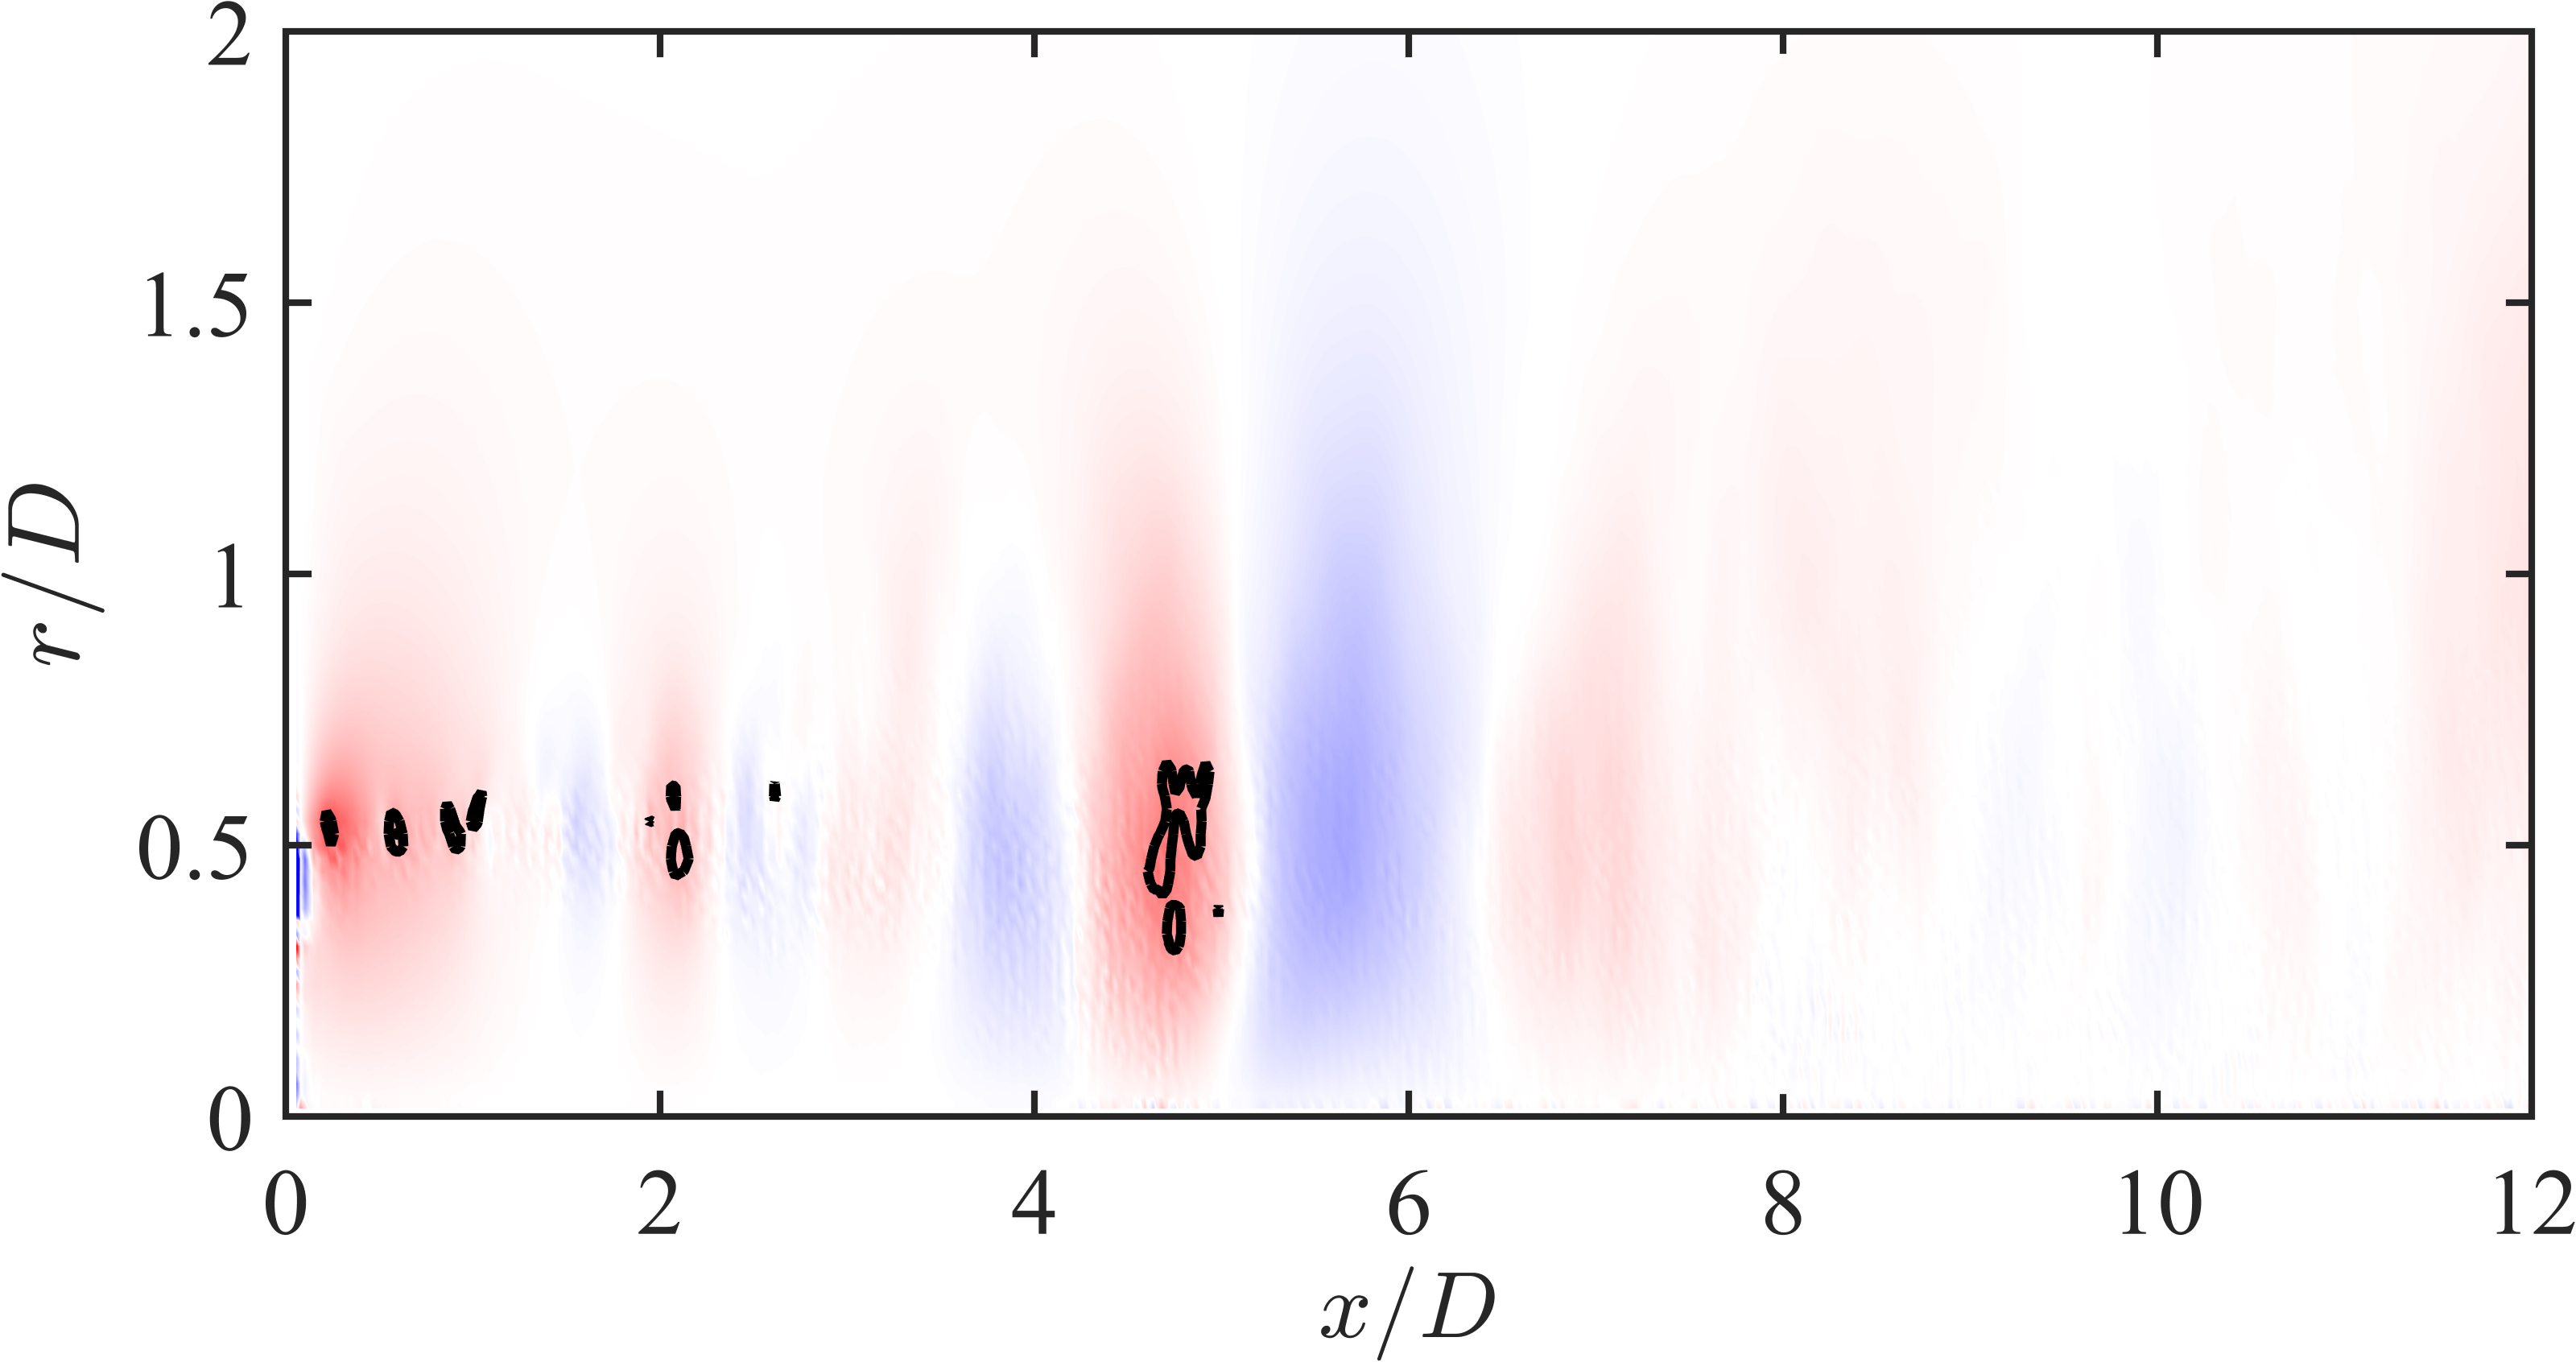
\includegraphics[width=0.65\linewidth]{Figures/ch5_St005_PSL_161.png}
%		\caption{$\phi = 7 \pi /8$}
%	\end{subfigure}
	\caption{Pseudo-pressure field induced by the large-scale structure ($St_{DF} = 0.05$) at two excitation instances, with swirling strength overlain in black contours. A consistent color map (of $\pm 4000$~Pa) and contour level are used for the two plots; regions of red indicate negative fluctuations.}
	\label{fig:PSL_St005}
\end{figure}
\begin{figure}
	\centering
	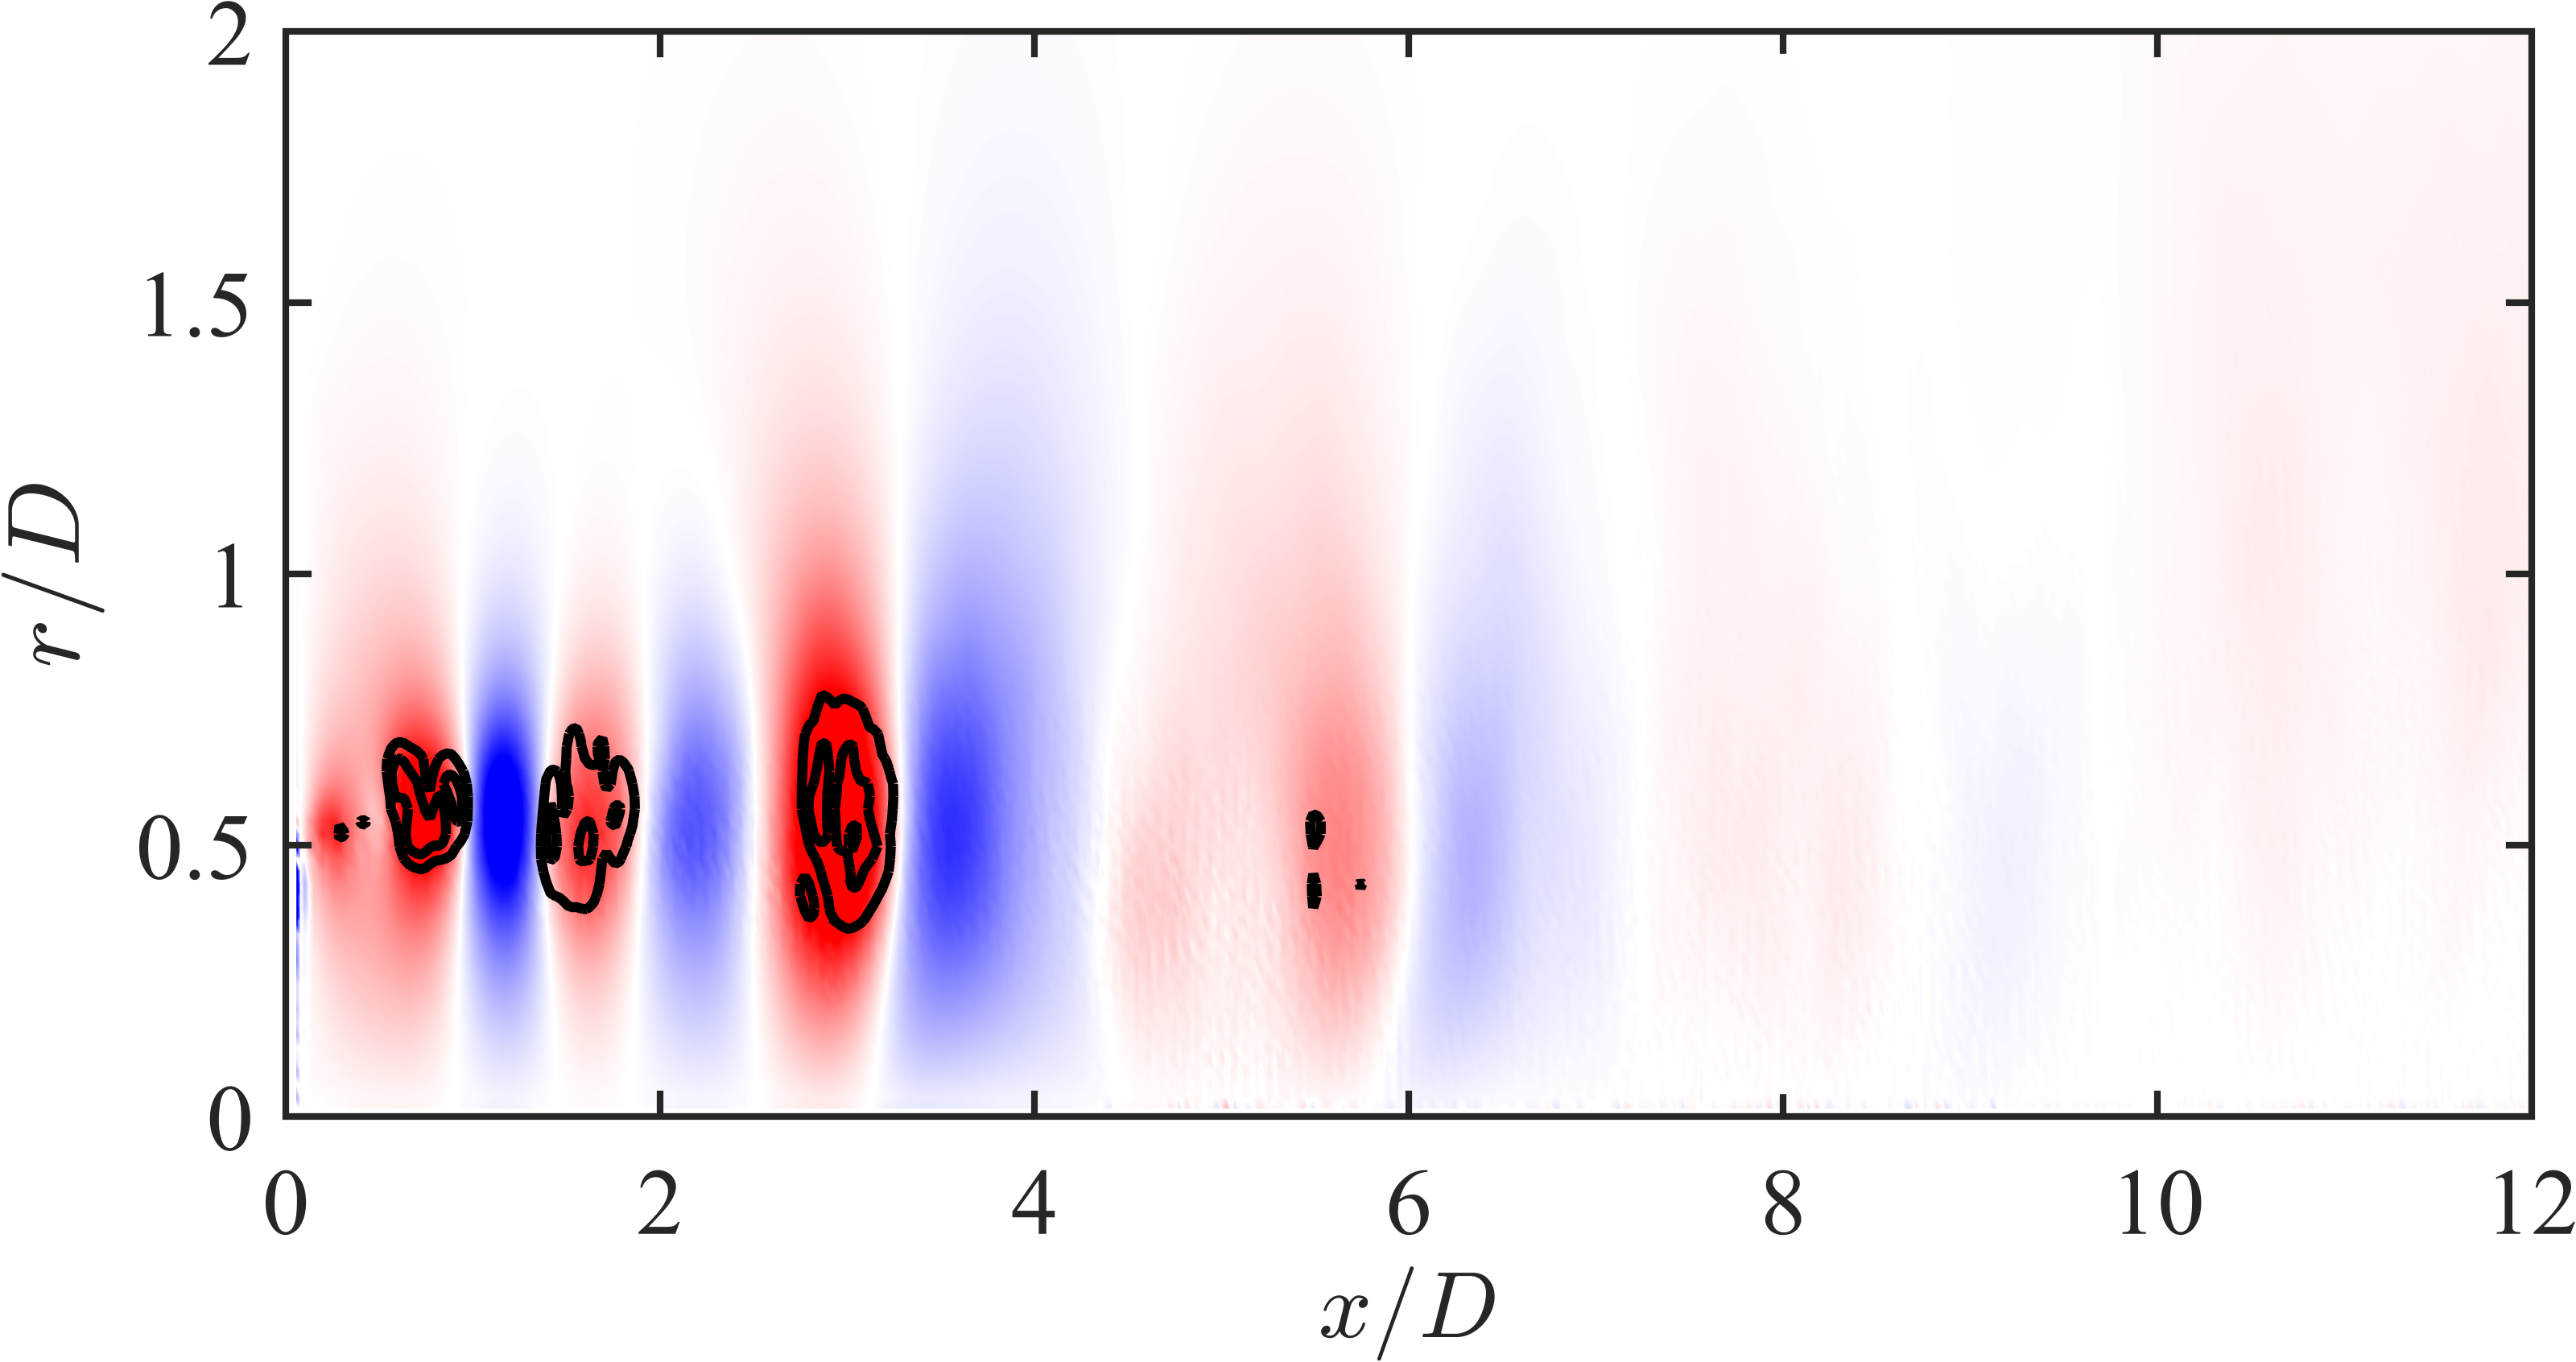
\includegraphics[width=0.65\linewidth]{Figures/ch5_St025_PSL_41.png}
	\caption{Pseudo-pressure field induced by the periodic large-scale structures ($St_{DF} = 0.25$) at an arbitrary phase.}
	\label{fig:PSL_St025}
\end{figure}

It should come as no surprise then that the aeroacoustic source would take the form of a wavepacket, centered around the coherent vortex.
This is shown in \fig{fig:SL} for both the impulsively- and periodically-excited structures.
Owing to the rapid growth and pairing process, the source field for the periodically-excited structures quickly amplifies and saturates by $x/D \simeq 2$.
In contrast, a slow amplification is observed for the impulsive structure, which reaches its maximum amplitude just before the vortex begins to decay. 
Based on the temporal extent of the acoustic response in the far-field, the acoustic wavelength of the emission produced by the individual ring vortex is $\sim 11D$, which would mean that the sources are non-compact per the results of \fig{fig:SL_St005}.
This is in general agreement with the analysis of \citet{Michalke1972}, which showed that the experimentally observed far-field spectral directivity could be reproduced using an axially-coherent, noncompact source model.
Of course, the amplitude of the source term alone does not determine acoustic emission; the acoustic emission is essentially the linear summation of the source/sink pairs (evaluated at retarded time) generated by the evolution of the vortices - a high amplitude source field coexisting with zero acoustic emission at a particular instant in time is therefore possible.
A rapid truncation of the source term therefore has the potential to significantly amplify the acoustic emission.
\begin{figure}
	\centering
%	\begin{subfigure}{0.75\textwidth}
%		\centering
		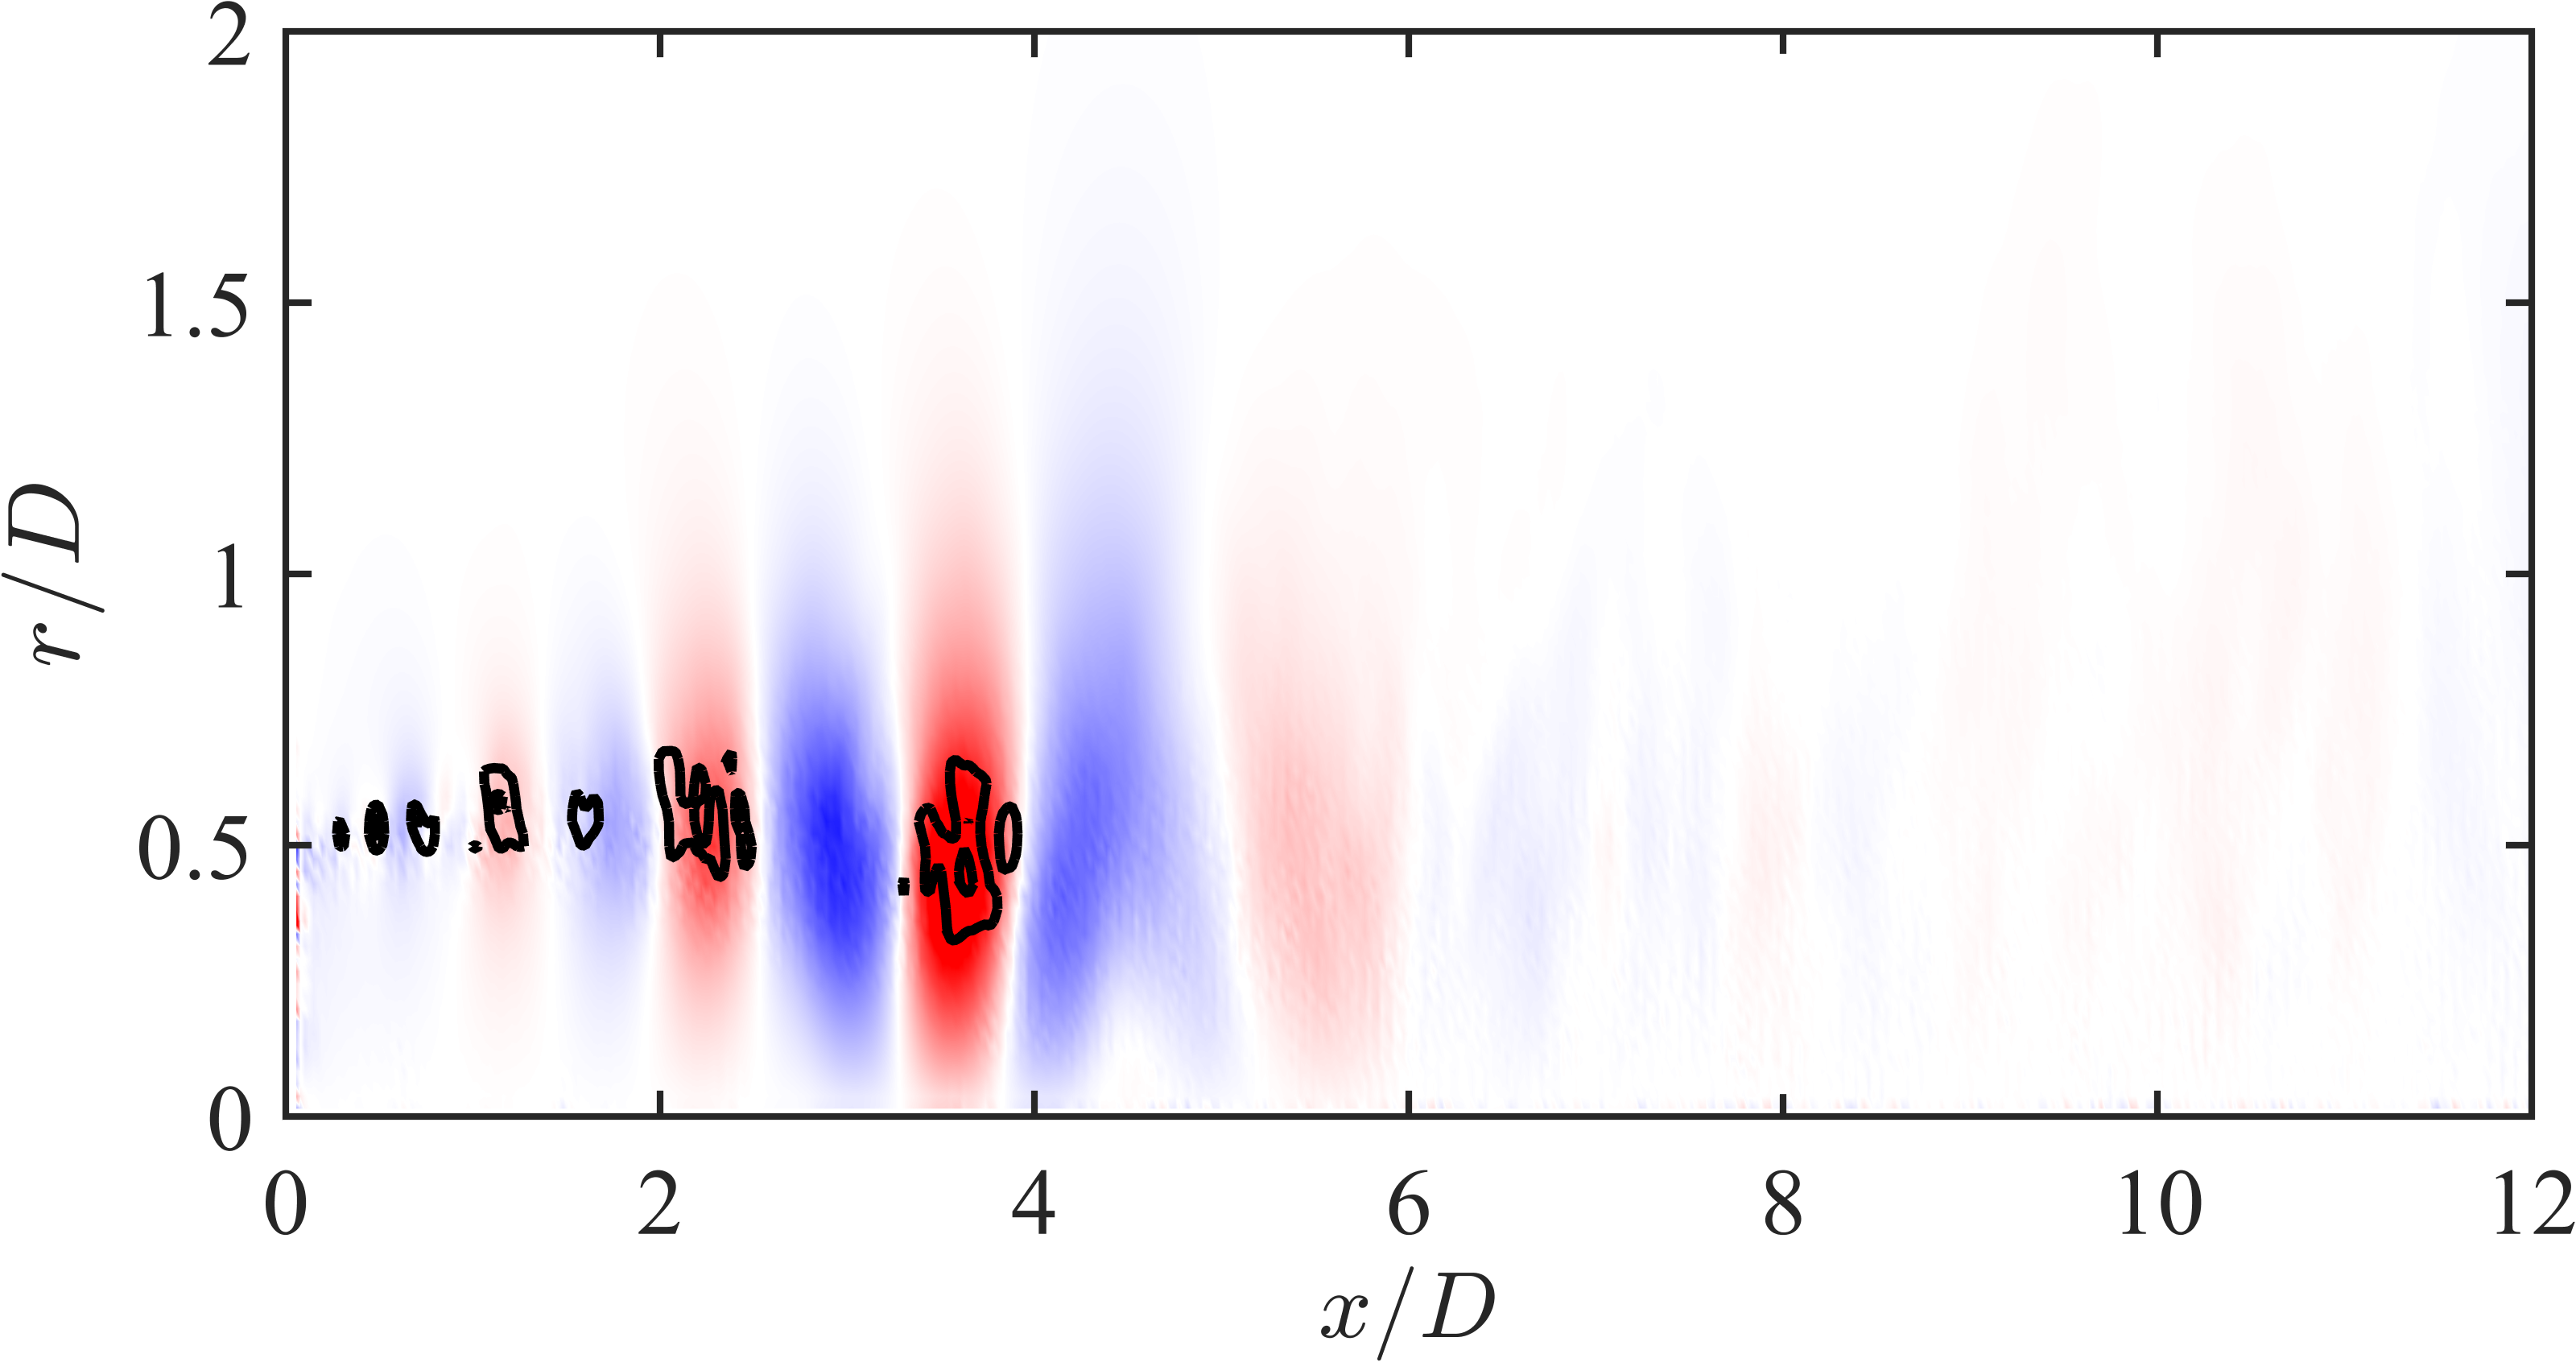
\includegraphics[width=0.65\linewidth]{Figures/ch5_St005_SL_131.png}\\
%		\caption{$St_{DF} = 0.05$}
%		\label{fig:SL_St005}
%	\end{subfigure}\\
%	\begin{subfigure}{0.75\textwidth}
%		\centering
		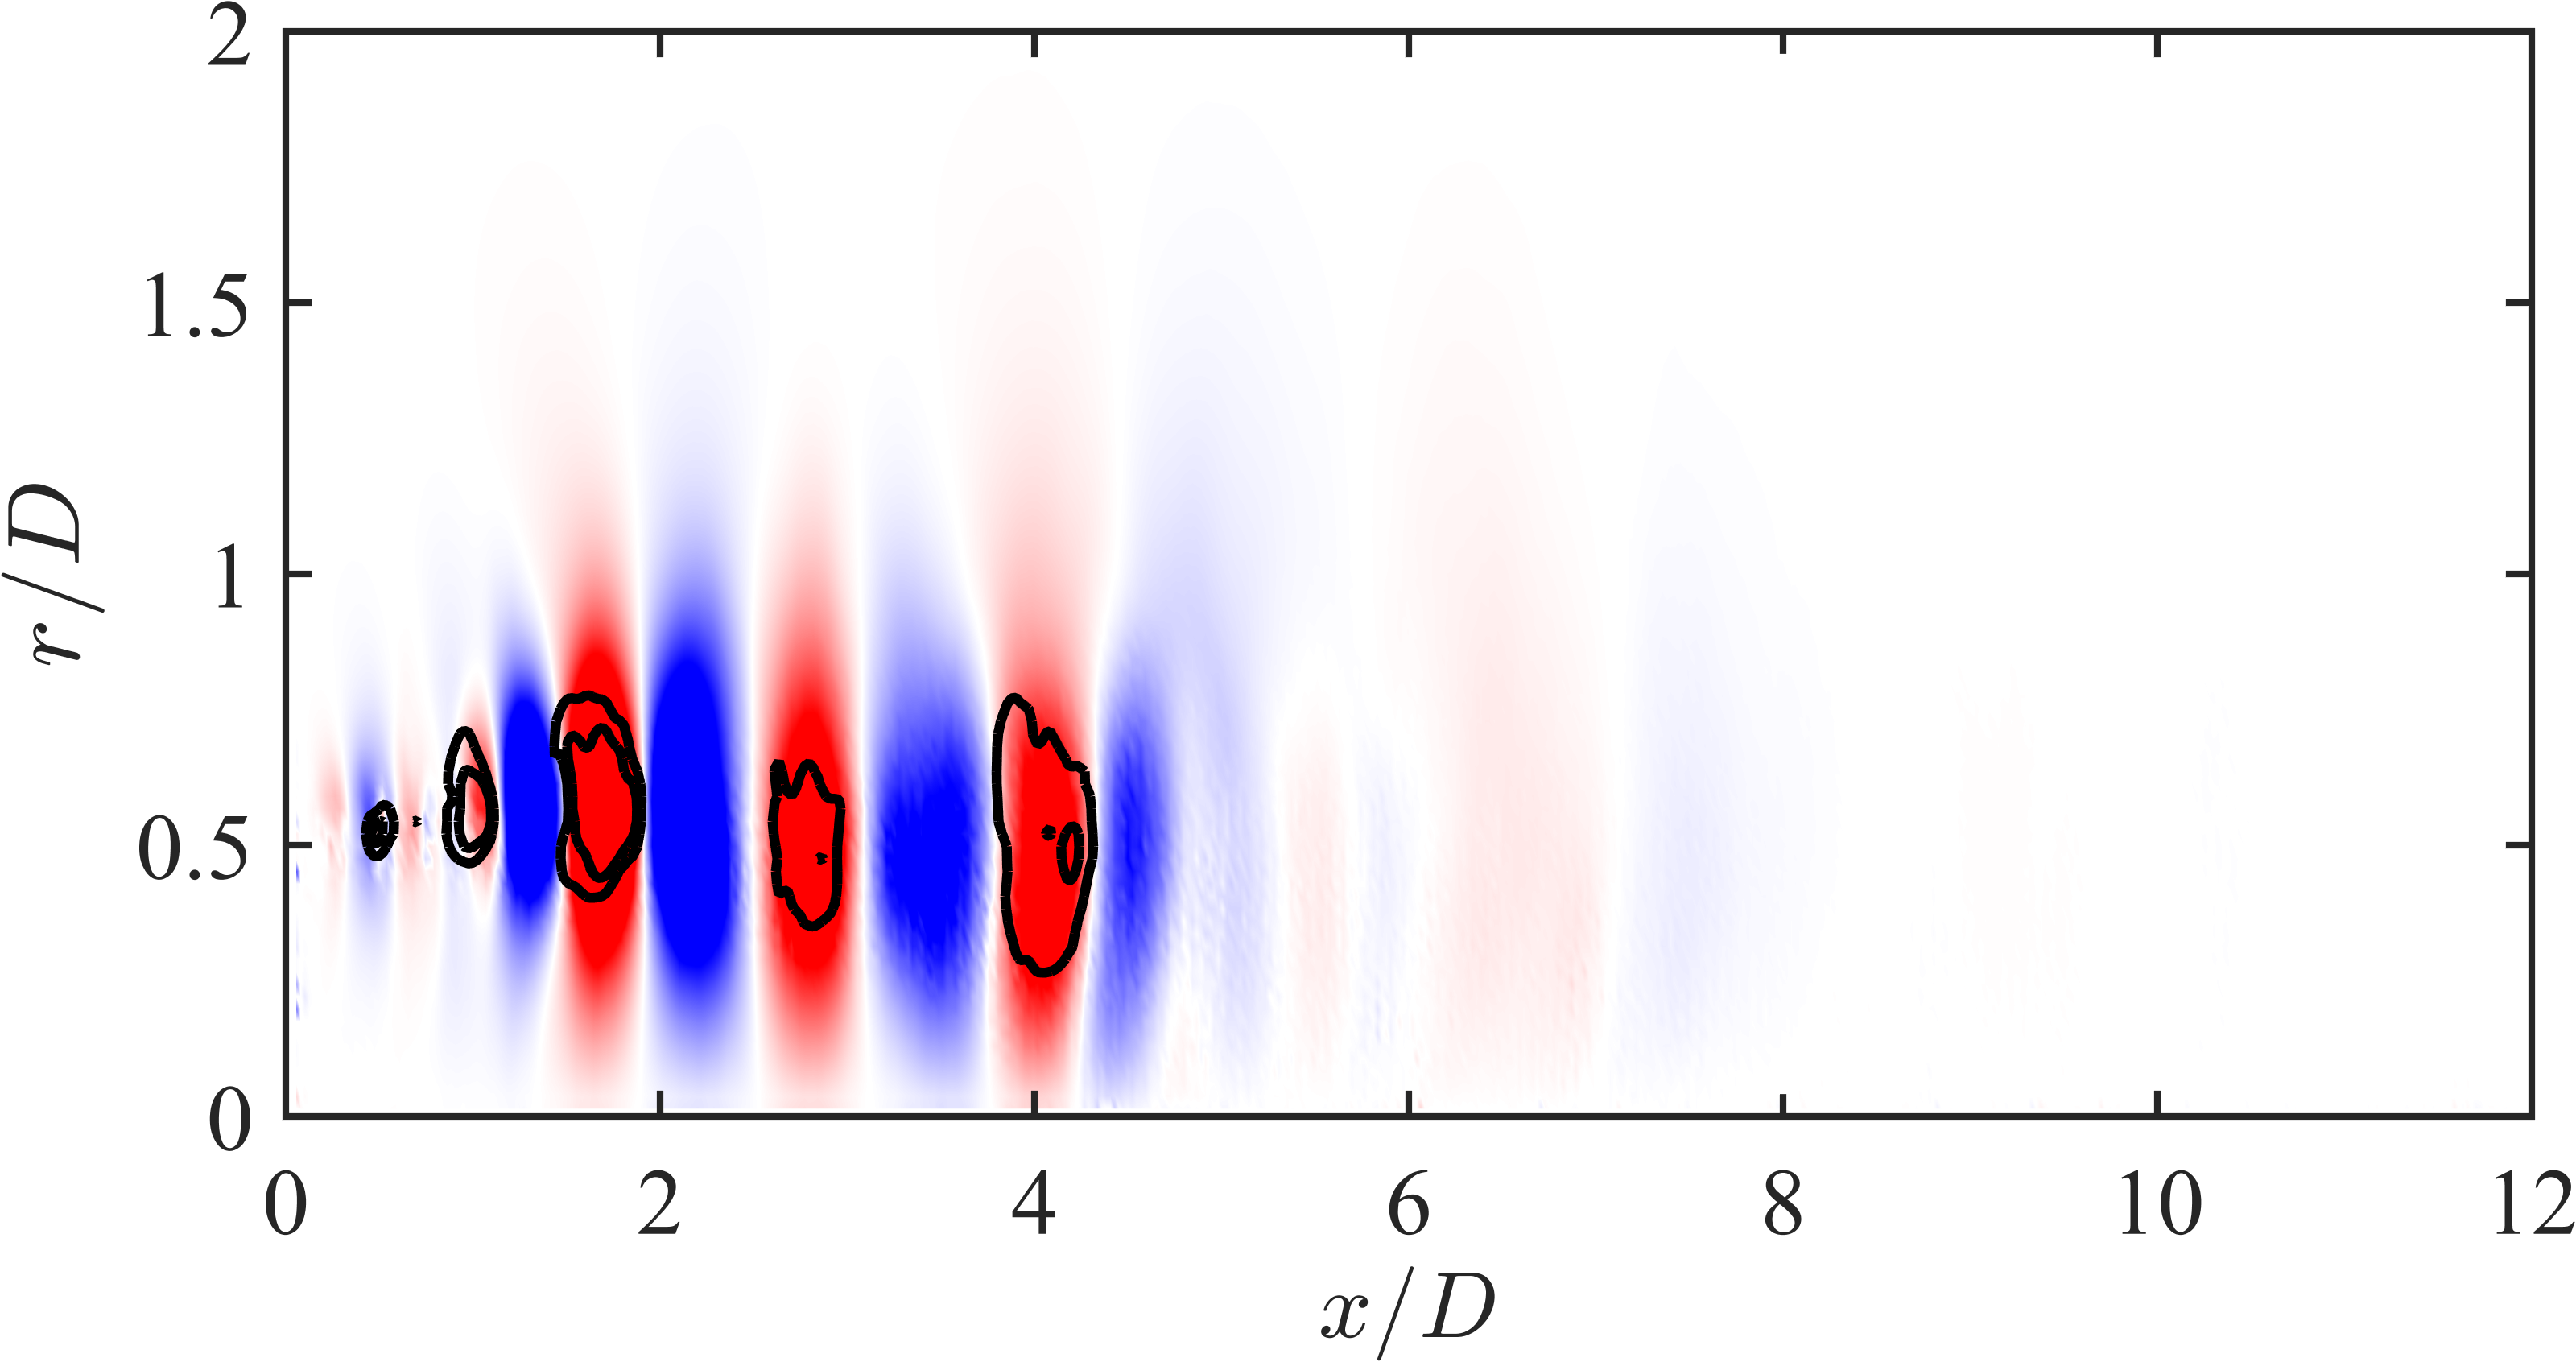
\includegraphics[width=0.65\linewidth]{Figures/ch5_St025_SL_1.png}
%		\caption{$St_{DF} = 0.25$}
%	\end{subfigure}
	\caption{Aeroacoustic source wavepackets induced by the large-scale structures. For readability, the colormap has been inverted from previous figures; here regions of red indicate positive fluctuations.}
	\label{fig:SL}
\end{figure}

This issue was explored in depth by \citet{Cavalieri2010} using analytic models for subsonic wavepackets.
By allowing the wavepacket amplitude and spatial extent to vary in time (termed `jittering'), the superdirective, intermittent acoustic emission pattern observed in high-speed jets was recovered and the predicted amplitude was within 1.5 dB of the measured.
A similar modulation of the spatial extent and amplitude of the source wavepackets can be observed here, depicted in \fig{fig:jittering}.
For the impulsively-excited jet, a single dominant acoustic source region is observed, modulated in space and time per the passage of the large-scale structures, and located at $ 2 \lesssim x/D \lesssim 6$.
As discussed previously, corresponds to the disintegration of the large-scale coherent vortices as they begin to self-interact near the end of the potential core.
For the $St_{DF} = 0.25$ excitation case, the overall amplitude of the acoustic source field is much higher than for the impulsively-excited case.
However, a similar modulation of the amplitude and spatial extent is observed here.
Unlike the impulsively-excited case however, the periodically-excited jet has, in addition to the downstream acoustic source, a high-intensity source region  for $x/D \lesssim 2$, corresponding to the pairing of the multiple harmonic structures generated per excitation pulse.
That the significant amplification of the fluctuating Reynolds' stress produced by the vortex merging is amplifying the source field, is unsurprising.
For this excitation frequency, the results of \sect{sect:nearfield} indicate that this is ultimately failing to significantly affect the far-field acoustic emission, at least at low polar angles.
\begin{figure}
	\centering
	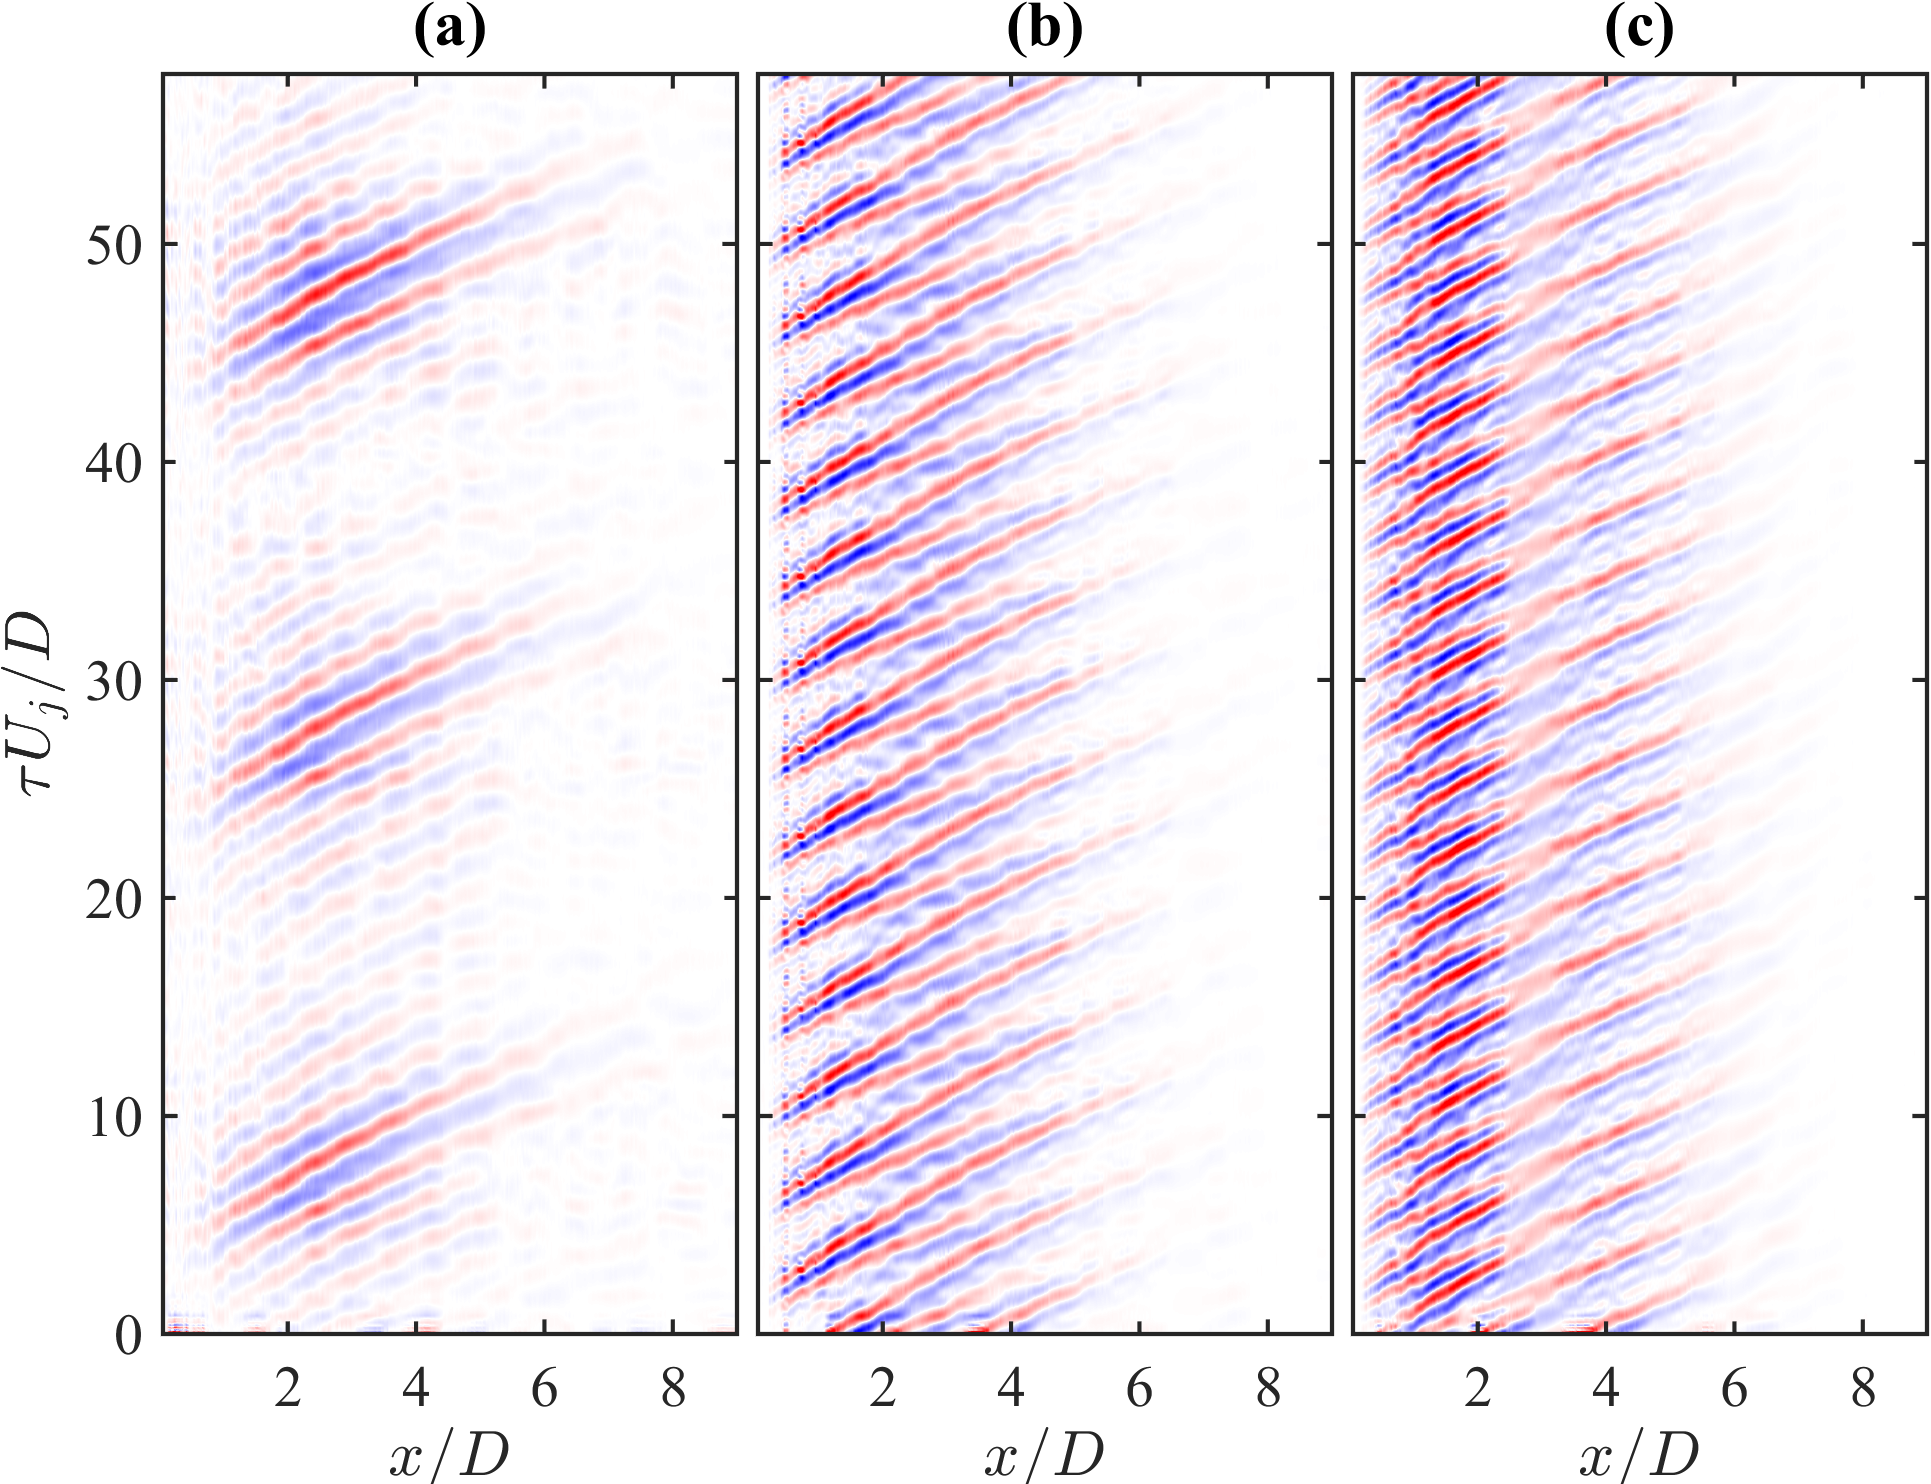
\includegraphics[width=0.9\linewidth]{Figures/sect_acoustic_source_modulated_source.png}
	\caption{Spatio-temporal modulation of the aeroacoustic source as measured along the lipline of the jet for $St_{DF} = 0.05$ (a), $0.25$ (b) and $0.35$ (c).}
	\label{fig:jittering}
\end{figure}

As the excitation frequency is further increased to $St_{DF} = 0.35$ however, the relative importance of the aeroacoustic source associated with the vortex merging is significantly increased.
The source field in the $St_{DF} = 0.35$ exhibits two highly distinctive regions in which the waveform undergoes a rapid modulation; this is in contrast to the results for $St_{DF} = 0.25$, where the source associated with the vortex merging and the source associated with the structure disintegration appear combined.
Vortex merging has been experimentally identified as acoustically important in low-speed, low-Reynolds number jets \citep{Kibens1980}.
The results of this section indicate that, under the right circumstances, vortex merging might also play a non-negligible role in the noise generation process in high-speed turbulent jets.
\section{Conclusions}
The aeroacoustic mechanisms in high-speed, turbulent jets were investigated using simultaneous pressure and velocity measurements of large-scale structures generated by plasma excitation of jet shear layer instabilities.
As the focus of this work was on mixing noise generated by turbulent shear layer structures common to all flow regimes, rather than acoustic emission generated by supersonic flow phenomena, an unheated, Mach 0.9 jet was used.
In the current work, only structures of azimuthal mode zero (axisymmetric ring vortices) were investigated. Previous researchers have identified the axisymmetric mode as the dominant acoustic emission pattern, and this also served to greatly simplify the data acquisition and analysis by eliminating the need to obtain azimuthal velocity components and gradients.

Previous work had identified an impulse response of the jet produced by very low frequency excitation ($St_{DF} \leq 0.05$), a periodic response of the jet produced by higher frequency excitation, and the linear relationship that existed between the two, both in the near-field pressure and the acoustic far-field.
New analysis of the near-field pressure used a wavelet--conditioning technique to extract the coherent signatures for the excited and natural jets.
Results showed clear similarities between the evolution of the signatures of the impulsively-excited structures and that of the natural jet.
The irrotational near-field pressure was then linearly decomposed into its constitutive hydrodynamic and acoustic components via a two-dimensional, spatio-temporal wavelet transform.
Once decomposed, linear correlations between the far-field acoustic signal at $30^\circ$ and the acoustic component of the near-field were computed in order to identify the dominant acoustic source region in the jet based on the measured time-lag for the peak correlation.
In all cases, natural and excited jets, the dominant acoustic source region was found to comprise the upstream region of the jet and end at $x/D \simeq 4$, just upstream of the end of the potential core.
This analysis is meant to identify only the dominant noise source region, and does not mean that no noise is generated outside of this region.
This result is in general accordance with previous results acquired at the GDTL by \citet{Hileman2005}, which identified the acoustic source region using delay-and-sum beamforming with a circular microphone array in the acoustic near-field (that is, far enough such that hydrodynamic pressure effects are negligible, but not in the true geometric far-field of the jet).
In that work, the dominant acoustic source region for an unheated, Mach 1.3 jet was found to be located just downstream of the end of the potential core, and was related to the breakup of large-scale coherent structures as they passed through this region.

The evolution, interactions, and, disintegration of the large-scale structures induced by the plasma excitation were then studied by stochastically-estimating the time-resolved velocity fields from ensemble acquisition of temporally-correlated velocity snapshots and near-field pressure traces.
The velocity snapshots were first decomposed into POD modes and a mapping from the near-field pressure to the POD expansion coefficients was generated by a standard feedforward, backpropagating neural network.
From this, the time-resolved expansion coefficients could be estimated and thus a reduced-order, time-resolved estimate of the velocity field produced.
Results showed that at very low excitation frequencies (impulsive excitation) each plasma pulse generates a single dominant structure, which initially grows rapidly as it convects downstream. 
As the structure nears the end of the potential core, $x/D \simeq 4$, a rapid disintegration of the vortex is observed, coincident with a strong axial acceleration.
As the excitation frequency is increased, a much more complex structure evolution takes form.
At moderate excitation frequencies (periodic forcing), multiple structures are initially formed by the plasma pulse; this is due to the higher-harmonics of the excitation pulse coupling with the most unstable shear layer frequency.
These initial, high-frequency structures quickly undergo a merging process (or multiple mergings) which ultimately produces large-scale coherent structures which are periodic and match the fundamental excitation frequency.
These large-scale structures later undergo a rapid disintegration and acceleration, similar to the impulsive excitation structures, as they convect downstream near the end of the potential core. 

Finally, the aeroacoustic sources were estimated from the time-resolved velocity fields using Ribner's simplified form of Lighthill's acoustic analogy.
This required numerous simplifications to the governing equations, which ultimately degraded the accuracy of the computed aeroacoustic source field.
Unfortunately, this limited interpretation of the results, as the computed far-field acoustic signal did not match well with the measured signal.
The algorithm did reproduce fluctuating acoustic fields of similar amplitude to what was measured experimentally, but the shape of the waveforms only matched in a rough sense.
Fortunately though, broad characteristic changes in the aeroacoustic source fields with excitation could still be identified.
The source fields indicated that the coherent structures produced a convected wavepacket-like event, centered on the jet lipline though reaching into the potential core.
For the individual vortex rings, a clear modulation of the spatial extent and amplitude was observed just upstream of the end of the potential core.
This corresponds to the location at which the coherent ring vortex underwent a rapid disintegration as well as acceleration, and corresponds to the location at which the dominant noise events are emitted per the two-point correlations between the acoustic component of the near-field pressure and the far-field at low polar angles.
For the periodically-excited jet, an additional noise source region is observed, corresponding to the location at which the multiple smaller-scale structures undergo a consistent merging thanks to the highly consistent vortex generation by the excitation.
This secondary source became more prominent as the excitation frequency increased to near the jet column mode frequency and the coherent vortices underwent two merging processes before decaying near the end of the potential core.

The linearity of the acoustic response of the jet (observed in the far-field) to impulsive and low-frequency periodic excitation ($St_{DF} \leq 0.25$), coupled with the observations of the vortex dynamics and acoustic source fields, indicates that the dominant source mechanism for these structures is the rapid modulation of the waveform brought on by the disintegration and acceleration of the large-scale structure as it begins to self-interact near the end of the potential core.
For the unexcited jet, in which ring vortices are highly unstable in the initial shear layer but the large-scale structures have a broad range of frequencies and phase relations to each other (and hence have less chance to merge repeatably), this is likely the dominant noise source mechanism. 
As the excitation frequency increased (to $St_{DF} \simeq 0.35$, which is near the jet column mode frequency), the secondary source mechanism associated with the vortex pairing becomes non-negligible, which results in a modification of the far-field response as it is now a combination of these two source mechanisms.
However, given the broadband nature of the jet turbulence (in terms of both temporal and azimuthal structure), it is unlikely that the vortex merging noise source mechanism is commonly encountered in the highly turbulent jet on a regular basis.
Ultimately, this work indicates that noise suppression may be achieved by seeding the growth of higher-order azimuthal modes, thereby limiting the growth of large-scale coherent structures, which will not undergo a rapid disintegration at the end of the potential core.  

%Acknowledgements should be included at the end of the paper, before the References section or any appendicies, and should be a separate paragraph without a heading. Several anonymous individuals are thanked for contributions to these instructions.

\bibliographystyle{jfm}
\bibliography{master.bib}

\end{document}
